% Options for packages loaded elsewhere
\PassOptionsToPackage{unicode}{hyperref}
\PassOptionsToPackage{hyphens}{url}
\PassOptionsToPackage{dvipsnames,svgnames,x11names}{xcolor}
%
\documentclass[
  letterpaper,
  DIV=11,
  numbers=noendperiod]{scrreprt}

\usepackage{amsmath,amssymb}
\usepackage{lmodern}
\usepackage{iftex}
\ifPDFTeX
  \usepackage[T1]{fontenc}
  \usepackage[utf8]{inputenc}
  \usepackage{textcomp} % provide euro and other symbols
\else % if luatex or xetex
  \usepackage{unicode-math}
  \defaultfontfeatures{Scale=MatchLowercase}
  \defaultfontfeatures[\rmfamily]{Ligatures=TeX,Scale=1}
\fi
% Use upquote if available, for straight quotes in verbatim environments
\IfFileExists{upquote.sty}{\usepackage{upquote}}{}
\IfFileExists{microtype.sty}{% use microtype if available
  \usepackage[]{microtype}
  \UseMicrotypeSet[protrusion]{basicmath} % disable protrusion for tt fonts
}{}
\makeatletter
\@ifundefined{KOMAClassName}{% if non-KOMA class
  \IfFileExists{parskip.sty}{%
    \usepackage{parskip}
  }{% else
    \setlength{\parindent}{0pt}
    \setlength{\parskip}{6pt plus 2pt minus 1pt}}
}{% if KOMA class
  \KOMAoptions{parskip=half}}
\makeatother
\usepackage{xcolor}
\setlength{\emergencystretch}{3em} % prevent overfull lines
\setcounter{secnumdepth}{5}
% Make \paragraph and \subparagraph free-standing
\ifx\paragraph\undefined\else
  \let\oldparagraph\paragraph
  \renewcommand{\paragraph}[1]{\oldparagraph{#1}\mbox{}}
\fi
\ifx\subparagraph\undefined\else
  \let\oldsubparagraph\subparagraph
  \renewcommand{\subparagraph}[1]{\oldsubparagraph{#1}\mbox{}}
\fi

\usepackage{color}
\usepackage{fancyvrb}
\newcommand{\VerbBar}{|}
\newcommand{\VERB}{\Verb[commandchars=\\\{\}]}
\DefineVerbatimEnvironment{Highlighting}{Verbatim}{commandchars=\\\{\}}
% Add ',fontsize=\small' for more characters per line
\usepackage{framed}
\definecolor{shadecolor}{RGB}{241,243,245}
\newenvironment{Shaded}{\begin{snugshade}}{\end{snugshade}}
\newcommand{\AlertTok}[1]{\textcolor[rgb]{0.68,0.00,0.00}{#1}}
\newcommand{\AnnotationTok}[1]{\textcolor[rgb]{0.37,0.37,0.37}{#1}}
\newcommand{\AttributeTok}[1]{\textcolor[rgb]{0.40,0.45,0.13}{#1}}
\newcommand{\BaseNTok}[1]{\textcolor[rgb]{0.68,0.00,0.00}{#1}}
\newcommand{\BuiltInTok}[1]{\textcolor[rgb]{0.00,0.23,0.31}{#1}}
\newcommand{\CharTok}[1]{\textcolor[rgb]{0.13,0.47,0.30}{#1}}
\newcommand{\CommentTok}[1]{\textcolor[rgb]{0.37,0.37,0.37}{#1}}
\newcommand{\CommentVarTok}[1]{\textcolor[rgb]{0.37,0.37,0.37}{\textit{#1}}}
\newcommand{\ConstantTok}[1]{\textcolor[rgb]{0.56,0.35,0.01}{#1}}
\newcommand{\ControlFlowTok}[1]{\textcolor[rgb]{0.00,0.23,0.31}{#1}}
\newcommand{\DataTypeTok}[1]{\textcolor[rgb]{0.68,0.00,0.00}{#1}}
\newcommand{\DecValTok}[1]{\textcolor[rgb]{0.68,0.00,0.00}{#1}}
\newcommand{\DocumentationTok}[1]{\textcolor[rgb]{0.37,0.37,0.37}{\textit{#1}}}
\newcommand{\ErrorTok}[1]{\textcolor[rgb]{0.68,0.00,0.00}{#1}}
\newcommand{\ExtensionTok}[1]{\textcolor[rgb]{0.00,0.23,0.31}{#1}}
\newcommand{\FloatTok}[1]{\textcolor[rgb]{0.68,0.00,0.00}{#1}}
\newcommand{\FunctionTok}[1]{\textcolor[rgb]{0.28,0.35,0.67}{#1}}
\newcommand{\ImportTok}[1]{\textcolor[rgb]{0.00,0.46,0.62}{#1}}
\newcommand{\InformationTok}[1]{\textcolor[rgb]{0.37,0.37,0.37}{#1}}
\newcommand{\KeywordTok}[1]{\textcolor[rgb]{0.00,0.23,0.31}{#1}}
\newcommand{\NormalTok}[1]{\textcolor[rgb]{0.00,0.23,0.31}{#1}}
\newcommand{\OperatorTok}[1]{\textcolor[rgb]{0.37,0.37,0.37}{#1}}
\newcommand{\OtherTok}[1]{\textcolor[rgb]{0.00,0.23,0.31}{#1}}
\newcommand{\PreprocessorTok}[1]{\textcolor[rgb]{0.68,0.00,0.00}{#1}}
\newcommand{\RegionMarkerTok}[1]{\textcolor[rgb]{0.00,0.23,0.31}{#1}}
\newcommand{\SpecialCharTok}[1]{\textcolor[rgb]{0.37,0.37,0.37}{#1}}
\newcommand{\SpecialStringTok}[1]{\textcolor[rgb]{0.13,0.47,0.30}{#1}}
\newcommand{\StringTok}[1]{\textcolor[rgb]{0.13,0.47,0.30}{#1}}
\newcommand{\VariableTok}[1]{\textcolor[rgb]{0.07,0.07,0.07}{#1}}
\newcommand{\VerbatimStringTok}[1]{\textcolor[rgb]{0.13,0.47,0.30}{#1}}
\newcommand{\WarningTok}[1]{\textcolor[rgb]{0.37,0.37,0.37}{\textit{#1}}}

\providecommand{\tightlist}{%
  \setlength{\itemsep}{0pt}\setlength{\parskip}{0pt}}\usepackage{longtable,booktabs,array}
\usepackage{calc} % for calculating minipage widths
% Correct order of tables after \paragraph or \subparagraph
\usepackage{etoolbox}
\makeatletter
\patchcmd\longtable{\par}{\if@noskipsec\mbox{}\fi\par}{}{}
\makeatother
% Allow footnotes in longtable head/foot
\IfFileExists{footnotehyper.sty}{\usepackage{footnotehyper}}{\usepackage{footnote}}
\makesavenoteenv{longtable}
\usepackage{graphicx}
\makeatletter
\def\maxwidth{\ifdim\Gin@nat@width>\linewidth\linewidth\else\Gin@nat@width\fi}
\def\maxheight{\ifdim\Gin@nat@height>\textheight\textheight\else\Gin@nat@height\fi}
\makeatother
% Scale images if necessary, so that they will not overflow the page
% margins by default, and it is still possible to overwrite the defaults
% using explicit options in \includegraphics[width, height, ...]{}
\setkeys{Gin}{width=\maxwidth,height=\maxheight,keepaspectratio}
% Set default figure placement to htbp
\makeatletter
\def\fps@figure{htbp}
\makeatother
\newlength{\cslhangindent}
\setlength{\cslhangindent}{1.5em}
\newlength{\csllabelwidth}
\setlength{\csllabelwidth}{3em}
\newlength{\cslentryspacingunit} % times entry-spacing
\setlength{\cslentryspacingunit}{\parskip}
\newenvironment{CSLReferences}[2] % #1 hanging-ident, #2 entry spacing
 {% don't indent paragraphs
  \setlength{\parindent}{0pt}
  % turn on hanging indent if param 1 is 1
  \ifodd #1
  \let\oldpar\par
  \def\par{\hangindent=\cslhangindent\oldpar}
  \fi
  % set entry spacing
  \setlength{\parskip}{#2\cslentryspacingunit}
 }%
 {}
\usepackage{calc}
\newcommand{\CSLBlock}[1]{#1\hfill\break}
\newcommand{\CSLLeftMargin}[1]{\parbox[t]{\csllabelwidth}{#1}}
\newcommand{\CSLRightInline}[1]{\parbox[t]{\linewidth - \csllabelwidth}{#1}\break}
\newcommand{\CSLIndent}[1]{\hspace{\cslhangindent}#1}

\KOMAoption{captions}{tableheading}
\makeatletter
\@ifpackageloaded{tcolorbox}{}{\usepackage[many]{tcolorbox}}
\@ifpackageloaded{fontawesome5}{}{\usepackage{fontawesome5}}
\definecolor{quarto-callout-color}{HTML}{909090}
\definecolor{quarto-callout-note-color}{HTML}{0758E5}
\definecolor{quarto-callout-important-color}{HTML}{CC1914}
\definecolor{quarto-callout-warning-color}{HTML}{EB9113}
\definecolor{quarto-callout-tip-color}{HTML}{00A047}
\definecolor{quarto-callout-caution-color}{HTML}{FC5300}
\definecolor{quarto-callout-color-frame}{HTML}{acacac}
\definecolor{quarto-callout-note-color-frame}{HTML}{4582ec}
\definecolor{quarto-callout-important-color-frame}{HTML}{d9534f}
\definecolor{quarto-callout-warning-color-frame}{HTML}{f0ad4e}
\definecolor{quarto-callout-tip-color-frame}{HTML}{02b875}
\definecolor{quarto-callout-caution-color-frame}{HTML}{fd7e14}
\makeatother
\makeatletter
\makeatother
\makeatletter
\@ifpackageloaded{bookmark}{}{\usepackage{bookmark}}
\makeatother
\makeatletter
\@ifpackageloaded{caption}{}{\usepackage{caption}}
\AtBeginDocument{%
\ifdefined\contentsname
  \renewcommand*\contentsname{Table of contents}
\else
  \newcommand\contentsname{Table of contents}
\fi
\ifdefined\listfigurename
  \renewcommand*\listfigurename{List of Figures}
\else
  \newcommand\listfigurename{List of Figures}
\fi
\ifdefined\listtablename
  \renewcommand*\listtablename{List of Tables}
\else
  \newcommand\listtablename{List of Tables}
\fi
\ifdefined\figurename
  \renewcommand*\figurename{Figure}
\else
  \newcommand\figurename{Figure}
\fi
\ifdefined\tablename
  \renewcommand*\tablename{Table}
\else
  \newcommand\tablename{Table}
\fi
}
\@ifpackageloaded{float}{}{\usepackage{float}}
\floatstyle{ruled}
\@ifundefined{c@chapter}{\newfloat{codelisting}{h}{lop}}{\newfloat{codelisting}{h}{lop}[chapter]}
\floatname{codelisting}{Listing}
\newcommand*\listoflistings{\listof{codelisting}{List of Listings}}
\makeatother
\makeatletter
\@ifpackageloaded{caption}{}{\usepackage{caption}}
\@ifpackageloaded{subcaption}{}{\usepackage{subcaption}}
\makeatother
\makeatletter
\@ifpackageloaded{tcolorbox}{}{\usepackage[many]{tcolorbox}}
\makeatother
\makeatletter
\@ifundefined{shadecolor}{\definecolor{shadecolor}{rgb}{.97, .97, .97}}
\makeatother
\makeatletter
\makeatother
\ifLuaTeX
  \usepackage{selnolig}  % disable illegal ligatures
\fi
\IfFileExists{bookmark.sty}{\usepackage{bookmark}}{\usepackage{hyperref}}
\IfFileExists{xurl.sty}{\usepackage{xurl}}{} % add URL line breaks if available
\urlstyle{same} % disable monospaced font for URLs
\hypersetup{
  pdftitle={R入門},
  pdfauthor={xjorv},
  colorlinks=true,
  linkcolor={blue},
  filecolor={Maroon},
  citecolor={Blue},
  urlcolor={Blue},
  pdfcreator={LaTeX via pandoc}}

\title{R入門}
\author{xjorv}
\date{9/29/23}

\begin{document}
\maketitle
\ifdefined\Shaded\renewenvironment{Shaded}{\begin{tcolorbox}[sharp corners, boxrule=0pt, frame hidden, borderline west={3pt}{0pt}{shadecolor}, interior hidden, enhanced, breakable]}{\end{tcolorbox}}\fi

\renewcommand*\contentsname{Table of contents}
{
\hypersetup{linkcolor=}
\setcounter{tocdepth}{2}
\tableofcontents
}
\bookmarksetup{startatroot}

\hypertarget{ux306fux3058ux3081ux306b}{%
\chapter*{はじめに}\label{ux306fux3058ux3081ux306b}}
\addcontentsline{toc}{chapter}{はじめに}

\markboth{はじめに}{はじめに}

その昔(2000年代初頭)、Rを初めて学ぶときには、CRANのホームページから英語のマニュアルを入手し、読むしかありませんでした.いくつかのRの教科書がすでに出版されていましたが、多くの教科書はプログラミングの入門については取り扱っておらず、統計手法の使い方、高度な統計について、あるいはパッケージのマニュアルなどについての説明が記載されていました。2000年代初頭に大学生であった私にはRはとても難しく、英語のマニュアルも読めず、インターネットに落ちているコードをコピペしては自分のデータを入力し、使い方もよくわからずに統計の計算をしていたものでした。簡単な統計はExcelや、怪しげなフリーソフトを用いて行っていました。どのソフトにも手法がないような統計の手法にだけ、Rを用いたのです。

時は流れ、2010年代、私は再びRと向き合うことになりました。その当時、研究で得たデータに対して、最小二乗法を用いて回帰を行い、測定できないパラメータを計算したかったのです。当時は最小二乗法しか回帰の方法を知らず、最小二乗法を解くために\textbf{\href{https://www.ruby-lang.org/ja/}{Ruby}}を勉強していました。今から考えると無謀なことに,回帰で3つ以上のパラメータを求めたかったのです。Rubyでも最小二乗法で残差が計算できることは分かっていましたが、配列(Rでいうところのベクターみたいなもの)の計算には繰り返し計算を使うしかなく、最小二乗法を組むだけでも大変でした。最小二乗法で残差を計算しても、最小値を求めることがどうしてもできず、今でいうところのグリッドサーチで最小値を求めようとしていました。

グリッドサーチでは到底最小値が求まらないことは分かっていました。そこで、Rという、統計学の言語のことを思い出したのです。しかし、当時の私は海外におり、教科書を買うこともできませんでした。

その時、Rを学ぶ光明となったのは、\textbf{R-tips}というホームページでした。R-tipsはデザインこそ昔ながらのHTMLでしたが、Rを一から学ぶための情報がすべて含まれており、始めから最後まで読み通し、学ぶことでRの使い方を覚えることができました。その後、Rを用いてマイクロアレイ(今でいうところの高速シークエンサーによるmRNA発現解析のようなもの)のデータを取り扱うようになり、\href{https://www.iu.a.u-tokyo.ac.jp/~kadota/r.html}{\textbf{(Rで)マイクロアレイデータ解析}}というホームページに書かれているコードを読むようになりました。R-tipsで学んだことを参考に、「(Rで)マイクロアレイデータ解析」のコードを読み解き、やがて私はRがある程度使えるようになりました。この2つのホームページがあったから、私はRを使えるようになったと言えます。

そして時は流れ202X年、私はしがないサラリーマンになりました。\href{https://www.iu.a.u-tokyo.ac.jp/~kadota/r.html}{(Rで)マイクロアレイデータ解析}のホームページはまだ更新されており、生き残っています。しかし、R-tipsのホームページはもうありません。\href{https://www.amazon.co.jp/R-Tips-\%E7\%AC\%AC3\%E7\%89\%88-\%E3\%83\%87\%E3\%83\%BC\%E3\%82\%BF\%E8\%A7\%A3\%E6\%9E\%90\%E7\%92\%B0\%E5\%A2\%83R\%E3\%81\%AE\%E5\%9F\%BA\%E6\%9C\%AC\%E6\%8A\%80\%E3\%83\%BB\%E3\%82\%B0\%E3\%83\%A9\%E3\%83\%95\%E3\%82\%A3\%E3\%83\%83\%E3\%82\%AF\%E3\%82\%B9\%E6\%B4\%BB\%E7\%94\%A8\%E9\%9B\%86/dp/4274219585}{\textbf{R-tipsは教科書}}
になったのです。日本語でどこでも読めて、Rを一から学べるホームページはなくなってしまいました。今でこそ私は英語のマニュアルを読み、理解することができます。しかし、Rも英語も何も知らない若年の初学者であったなら、Rを学ぶことを躊躇したでしょう。もちろん、昔と比べるとRについての情報はネット上にたくさん転がっており、落穂ひろいしながらRを学んでいくことはできます。しかし、R-tipsがそうであったように、一つのホームページで、広告などもなく、いちいち検索することもなくRについての情報を一度に得ることは(教科書を除けば)できなくなってしまいました。

私も稀にRの初学者に使い方を教えようとすることがあります。しかし、一か所にRの基本的な使い方に関する情報が集まったような資料はあまりありません.プレゼンテーションで教えるにしても,プログラミング言語の学習にはプレゼンテーションはあまり向いていません。すべてをプレゼンテーションで伝えようとするととても時間がかかってしまいます。ですので、大したR使いではない私がこのようなものを作るのはどうかとは思いつつ、R-tipsのようなものを作ることにしました。

Rでホームページを作る、教科書を作ることは昔は現実的ではありませんでした。しかし、今ではRを使って簡単なWebアプリを作ったり、教科書を作ったりすることは比較的簡単にできます。この文書もRで作成しています。私が学び始めたときのように、統計しかできないプログラミング言語ではないのです。

とは言え、Rは統計のプログラミング言語です。Webを使った本格的なサービスを作りたい、データベースに保存されたデータを常時解析し、オンライン上でダッシュボードに表示したいなど、もっと複雑なことがしたいなら別の言語、例えば\textbf{\href{https://www.python.org/}{Python}}を学ぶとよいでしょう。\href{https://ja.wikipedia.org/wiki/\%E3\%82\%A2\%E3\%83\%89\%E3\%83\%9B\%E3\%83\%83\%E3\%82\%AF}{ad
hoc}な、その場一回限りの統計や計算こそ、Rが最も生きる場面です。眼の前にある統計データを解析したい、統計の手法を試したいというのであれば、Rは最適な言語のひとつであると言えます。

この文書を読むことによって、皆さんがRに親しみ、データやグラフを自由自在に扱えるようになれば、そして私がR-tipsに助けられたように、Rの初学者のためになれば、これ以上の喜びはありません。

\begin{quote}
R-tipsが私にとってのRの入門になりましたが、Rubyに入門した時には\href{https://www.amazon.co.jp/\%E3\%81\%9F\%E3\%81\%AE\%E3\%81\%97\%E3\%81\%84Ruby-\%E7\%AC\%AC6\%E7\%89\%88-Informatics-IDEA-\%E9\%AB\%98\%E6\%A9\%8B/dp/4797399848}{\textbf{「たのしいRuby」}}を用いて学びました。この文書は、プログラミングへの入門編として、なるべく「たのしいRuby」に記載された内容に沿って記載していきます。
\end{quote}

\hypertarget{ux8a18ux8f09ux306eux65b9ux91dd}{%
\section*{記載の方針}\label{ux8a18ux8f09ux306eux65b9ux91dd}}
\addcontentsline{toc}{section}{記載の方針}

\markright{記載の方針}

このページでは,基本的にプログラミング初学者を対象として,プログラミングの基礎から統計・グラフ作成の基礎までを取り扱います.複雑な統計手法については,別の資料を参照しつつ,紹介程度に留めます.

普通の教科書では,同じ内容を複数の章に繰り返し記載することは避けます.紙に印刷する教科書では,反復があるとそれだけ教科書が厚くなり,持ち運びにも印刷等のコスト面にもデメリットがあります.しかし,オンラインの無料の教科書ではこのようなコストはほぼ無視できます.

同じ内容を何度も繰り返すうちに,物事は自然と憶えられるものです.家から学校までの道のりを初めて通る時には道に迷うこともありますが,何度も往復を繰り返すうちに道を憶え,間違えなくなります.学習でも同じことが起こります.このページでは,重要な内容は繰り返し出てくるような記載にしています.何度も同じことを目に入れることで,記憶が定着し,その内容を覚えられることを期待したものです.

と,良くいうと上記のようなことになりますが,実際には重複を個人ですべて叩き潰すのは大変だからやっていない,というだけです.「この内容は前にも見たことがあるなあ」と思ったら,飛ばして読んでもらっても特に問題はありません.

\hypertarget{ux8457ux4f5cux6a29ux306bux3064ux3044ux3066}{%
\section*{著作権について}\label{ux8457ux4f5cux6a29ux306bux3064ux3044ux3066}}
\addcontentsline{toc}{section}{著作権について}

\markright{著作権について}

この文書はクリエイティブ・コモンズ
\href{https://creativecommons.org/licenses/by-nc-sa/4.0/deed.ja}{CC
BY-NC-SA}に従い,複製、頒布、展示、実演を行うにあたり、著作権者の表示を要求し、非営利目的での利用に限定し、作品を改変・変形・加工してできた作品についても、元になった作品と同じライセンスを継承させた上で頒布を認めます。

元々無料の資料を提供することが目的であるため,非営利目的で,読みやすく,より良い資料に加工してもらえるのであれば,どのように利用していただいても問題ありません.

\bookmarksetup{startatroot}

\hypertarget{rux306eux30a4ux30f3ux30b9ux30c8ux30fcux30eb}{%
\chapter{Rのインストール}\label{rux306eux30a4ux30f3ux30b9ux30c8ux30fcux30eb}}

\hypertarget{rux306eux30a4ux30f3ux30b9ux30c8ux30fcux30eb-1}{%
\section{Rのインストール}\label{rux306eux30a4ux30f3ux30b9ux30c8ux30fcux30eb-1}}

Rを使い始める前に、まずはRをインストールする必要があります。まずは、\href{https://cran.r-project.org/}{\textbf{CRAN}}(The
Comprehensive R Archive
Network)というホームページからRのインストールを行います。ホームページの「Download
and Install
R」の部分から、ご自身のPC環境(Windows、MacOS、Linux)を選択します。

\begin{figure}

{\centering 
\includegraphics{././image/CRAN_install1.png}

}

\caption{図1:CRANのページ:Rのインストール}

\end{figure}

\hypertarget{windowsux3067ux306eux30a4ux30f3ux30b9ux30c8ux30fcux30eb}{%
\subsection{windowsでのインストール}\label{windowsux3067ux306eux30a4ux30f3ux30b9ux30c8ux30fcux30eb}}

Windowsであれば、上の図に示したリンクから次のページに移動し、さらに「base」を選択します。

\begin{figure}

{\centering 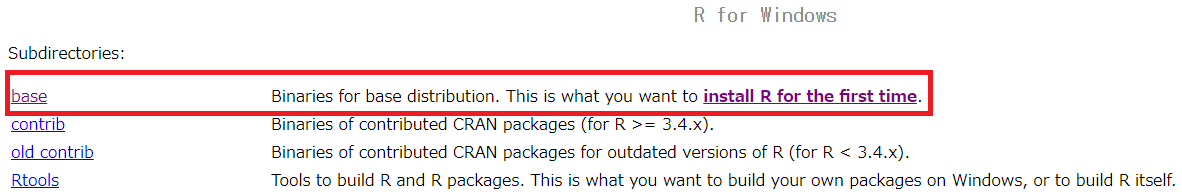
\includegraphics{././image/CRAN_install2_win.png}

}

\caption{図2:CRANのページ:Windowsでのインストール}

\end{figure}

移動すると、Rのダウンロードリンクが表示されますので、ココからRのインストーラーをダウンロードします。

\begin{figure}

{\centering 
\includegraphics{././image/CRAN_install3_win.png}

}

\caption{図3:CRANのページ:Windowsのインストールファイルのダウンロード}

\end{figure}

ダウンロードされたインストーラーを開き、「次へ」を押していけばインストールが完了します。

\begin{figure}

{\centering 
\includegraphics{././image/CRAN_install4_win.png}

}

\caption{図4:CRANのページ:インストーラーを起動した画面}

\end{figure}

\hypertarget{rtoolsux306eux30a4ux30f3ux30b9ux30c8ux30fcux30eb}{%
\subsubsection{Rtoolsのインストール}\label{rtoolsux306eux30a4ux30f3ux30b9ux30c8ux30fcux30eb}}

Rを使うときには、時にCのコードをコンパイル(機械語に変換)する必要があります。このような場合に用いられるのが\textbf{Rtools}です。図2で示したページに、「Rtools」というリンクがありますので、ココからRtoolsのページに移動します。移動するとRのバージョンに合わせたRtoolsへのリンクが表示されます。最新のRをインストールした場合には、Rtoolsも最新のRに対応したものになりますので、一番上のRtoolsのリンクを開きます。Rのバージョンが最新ではない場合には、Rのバージョンを確認した上で対応したRtoolsを選択します。

\begin{figure}

{\centering 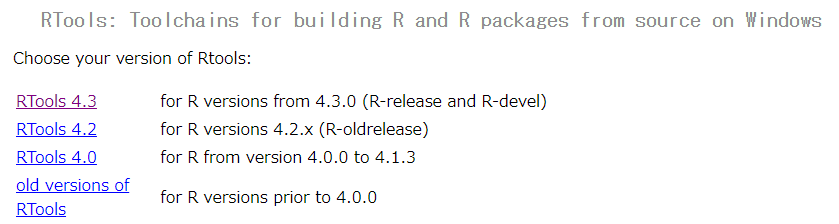
\includegraphics{././image/CRAN_install5_Rtools.png}

}

\caption{図5:CRANのページ:Rtools}

\end{figure}

Rのバージョンに対応したRtoolsのリンクに移動すると、下のように表示されます。Rtools
installerのリンクを開くと、Rtoolsのインストーラーがダウンロードされます。インストーラーを開いてRtoolsをインストールしましょう。

\begin{figure}

{\centering 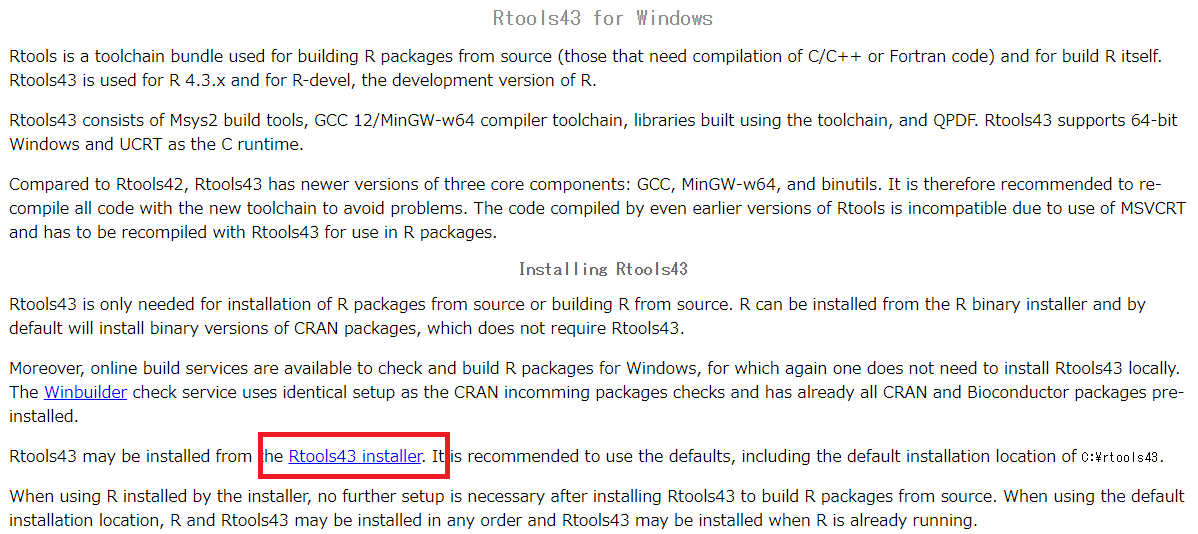
\includegraphics{././image/CRAN_install6_Rtools.png}

}

\caption{図6:CRANのページ:Rtoolsのインストーラーのダウンロード}

\end{figure}

\hypertarget{macosux3067ux306eux30a4ux30f3ux30b9ux30c8ux30fcux30eb}{%
\subsection{MacOSでのインストール}\label{macosux3067ux306eux30a4ux30f3ux30b9ux30c8ux30fcux30eb}}

MacOSの場合もWindowsと同じように、図1でMacOSのリンクを選択してインストーラーをダウンロードします。MacOSの場合はCPUによってインストーラーが異なります。Apple
Silicon(M1/M2)で動いているMacOS11以降のMacでは、上のリンクを選択してダウンロードし、IntelのCPUで動いているMacの場合は下のリンクを選択してダウンロードします。インストーラーを起動すると、Rと同じようにRをインストールすることができます。

\begin{figure}

{\centering 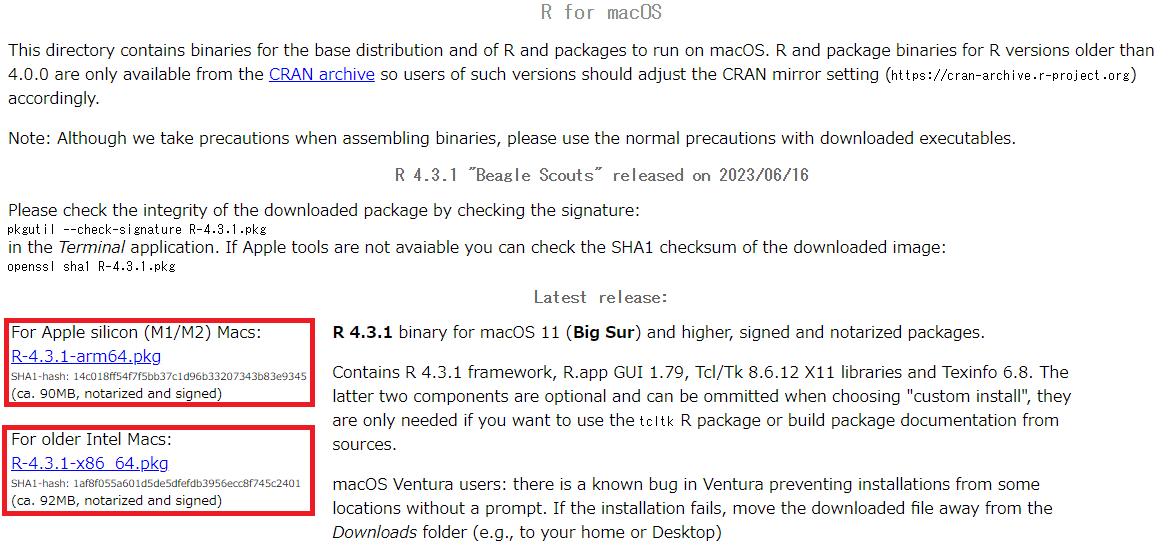
\includegraphics{././image/CRAN_install7_mac.png}

}

\caption{図6:CRANのページ:Rtoolsのインストーラーのダウンロード}

\end{figure}

\hypertarget{linuxux3067ux306eux30a4ux30f3ux30b9ux30c8ux30fcux30eb}{%
\subsection{Linuxでのインストール}\label{linuxux3067ux306eux30a4ux30f3ux30b9ux30c8ux30fcux30eb}}

Linuxでのインストールでは、特にCRANのホームページに移動してダウンロードを行う必要はありません。apt
install(Ubuntuの場合)でRをインストールするだけです。

\begin{Shaded}
\begin{Highlighting}[]
\NormalTok{sudo apt update}
\NormalTok{sudo apt install r{-}base}
\end{Highlighting}
\end{Shaded}

\hypertarget{rstudioux306eux30a4ux30f3ux30b9ux30c8ux30fcux30eb}{%
\section{Rstudioのインストール}\label{rstudioux306eux30a4ux30f3ux30b9ux30c8ux30fcux30eb}}

Rには、\textbf{R
RGui}と呼ばれるインターフェースが始めから登録されています。Rを起動するとまず表示されるのはこのRGuiです。

\begin{figure}

{\centering 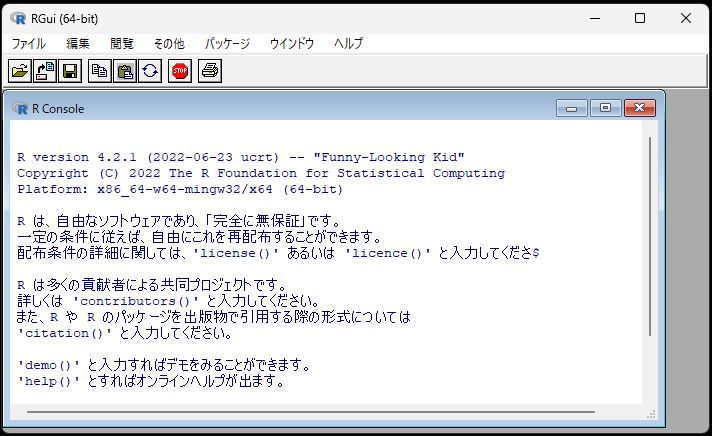
\includegraphics{././image/RGUI.png}

}

\caption{図7:RGui}

\end{figure}

このRGuiを用いて、Rでスクリプト(プログラム)を書いて、実行することができます。ただし、このRGuiはRが利用され始めてすぐに開発されたものであり、最近のプログラミング環境では標準的に備わっている、\textbf{シンタックスハイライト}(プログラムの要素によって色やフォントを変化させる機能)や\textbf{入力補助}(文書の一部を入力すると入力候補を提案してくれる機能)、\textbf{コードのバージョン管理}(\href{https://git-scm.com/}{git}などのバージョン管理ソフト)などの機能が備わっていません。このような機能を持つ、プログラミングを快適に行うための環境のことを、\textbf{統合開発環境(IDE、Integrated
Development Environment)}と呼びます。

統合開発環境として有名なのは、\href{https://www.gnu.org/software/emacs/}{Emacs}や\href{https://www.vim.org/}{Vim}、\href{https://azure.microsoft.com/ja-jp/products/visual-studio-code}{Visual
Studio
Code(VScode)}などです。これらはRだけでなく、他の言語もサポートしています。Rでは、ほぼR専用の統合開発環境として、\href{https://posit.co/products/open-source/rstudio/}{\textbf{RStudio}}というものがあります。
Rを使う時には、もちろんRGuiやEmacs、Vim、VScodeなどを用いても問題はありませんし、R言語だけでなく、他の言語(Pythonなど)を同時に利用するのであれば、むしろVScodeを利用する方が良いこともあります。ただし、Rを学び、Rで統計を行うのが主な目的であれば、RStudioを使うのが最もよいでしょう。

Rstudioは\href{https://posit.co/products/open-source/rstudio/}{\textbf{Posit}}のホームページからダウンロードすることができます。まず、Rを上記の手順でインストールし、その後、Rstudioのインストーラーを以下の図の手順でダウンロードしましょう。

\begin{figure}

{\centering 
\includegraphics{././image/Posit_Rstudio.png}

}

\caption{図8:Rstudioのダウンロード(右上からリンクへ移動)}

\end{figure}

\begin{figure}

{\centering 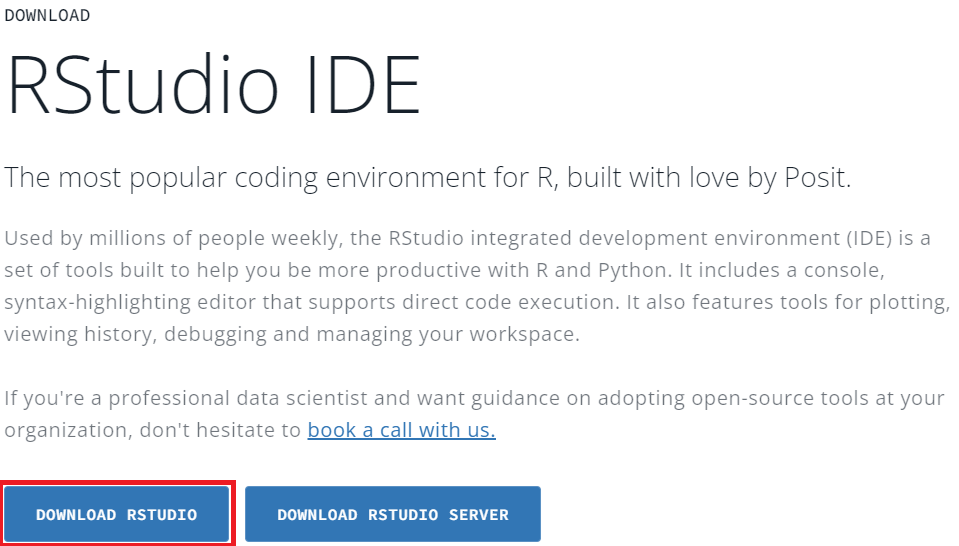
\includegraphics{././image/Posit_Rstudio2.png}

}

\caption{図9:Rstudioのダウンロード(左のリンクからダウンロード)}

\end{figure}

Rstudioのインストーラーを起動し、Rstudioがインストール出来たら準備は完了です。Rstudioを起動し、Rを使ってみましょう。

\bookmarksetup{startatroot}

\hypertarget{rux3092ux4f7fux3063ux3066ux307fux3088ux3046}{%
\chapter{Rを使ってみよう}\label{rux3092ux4f7fux3063ux3066ux307fux3088ux3046}}

RとRstudioをインストールしたら、さっそくRstudioを起動してみましょう。

\hypertarget{rstudioux306eux30d1ux30cdux30eb}{%
\section{Rstudioのパネル}\label{rstudioux306eux30d1ux30cdux30eb}}

Rstudioを開くと以下のような画面が表示されます。Rstudioでは、1つのウインドウの中に、4つのパネルが配置されます。ただし、インストールしてすぐに開くと、左側は1つのパネルになっているかもしれません。

\begin{figure}

{\centering 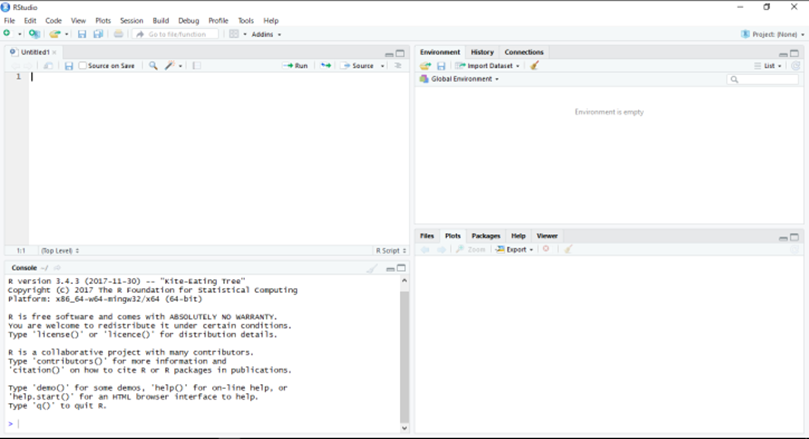
\includegraphics{././image/Rstudio1.png}

}

\caption{図1:Rstudioを開いたところ}

\end{figure}

Rstudioのそれぞれのパネルについて説明していきます。左上のパネル①は\textbf{テキストエディタ}と呼ばれるものです。テキストエディタにはプログラムを書き込んでいきます。書き込んだプログラムは、①の右上にある、\textbf{「run」}という部分を押すと実行されます。少し長めのプログラムを書く場合には、このテキストエディタを使用します。

左下のパネル②は\textbf{コンソール}と呼ばれる部分です。このコンソールには実行されたプログラムが表示されます。プログラムから何かを表示するよう指示した場合には、結果がこのコンソールに表示されます。Rでは、このコンソールに直接プログラムを書き込んで実行することもできます。1行程度のプログラムを直接書き込んで挙動を調べたり、今取り扱っているデータを確認するときには、このコンソールにプログラムを直接書き込みます。

このように、プログラムを直接書き込み、すぐに実行し、結果を得るような仕組みのことを\textbf{対話的プログラミング}と呼びます。対話的プログラミングは他のプログラミング言語にも備わっていますが、Rでは今書いているプログラムに干渉する形で対話的プログラミングを行うことができるという特徴があります。プログラミングでは、プログラムが思ったように動かない、バグが常に生じます。Rでは対話的プログラミングを通じてバグを修正し、プログラムが思った通りに動くよう修正していくことができます。

右上パネル③は現在Rが取り扱っている\textbf{オブジェクト}についての情報が表示されます。オブジェクトについては次の章で詳しく説明します。右下のパネル④には、Rで描写したグラフや、ヘルプ、フォルダの情報などが表示されます。

\begin{figure}

{\centering 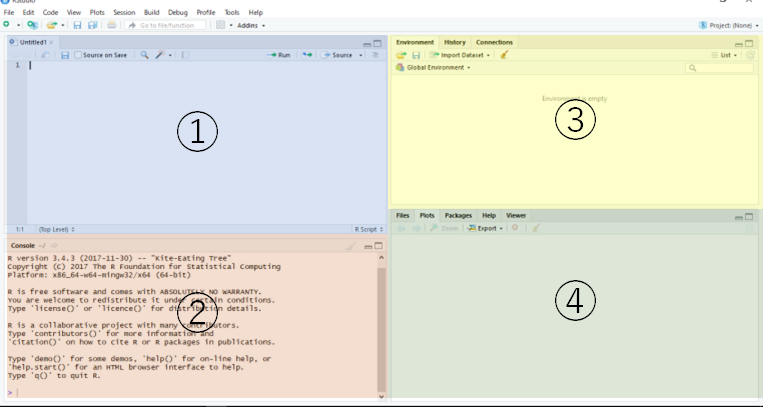
\includegraphics{././image/Rstudio2.png}

}

\caption{図2:Rstudioを開いたところ}

\end{figure}

\hypertarget{ux30b3ux30f3ux30bdux30fcux30ebux306bux5165ux529b}{%
\section{コンソールに入力}\label{ux30b3ux30f3ux30bdux30fcux30ebux306bux5165ux529b}}

では、まずコンソール、右下のパネル②に直接プログラムを書き込んでみましょう。とは言っても、書き込むプログラムは以下の通り、非常に簡単なものです。以下のプログラムをコピーペーストでコンソールに張り付け、エンターキーを押しましょう。

\begin{Shaded}
\begin{Highlighting}[]
\DecValTok{1} \SpecialCharTok{+} \DecValTok{1}
\end{Highlighting}
\end{Shaded}

\begin{verbatim}
[1] 2
\end{verbatim}

\begin{Shaded}
\begin{Highlighting}[]
\StringTok{"Hello World"}
\end{Highlighting}
\end{Shaded}

\begin{verbatim}
[1] "Hello World"
\end{verbatim}

プログラムの結果(出力)として、上に示したように「{[}1{]}
2」と、「{[}1{]} ``Hello
world''」と表示されたと思います。このように、簡単な計算や文字の表示程度であれば、エディタ(パネル①)に書き込まなくても実行することができます。

\hypertarget{ux30a8ux30c7ux30a3ux30bfux3092ux4f7fux3046}{%
\section{エディタを使う}\label{ux30a8ux30c7ux30a3ux30bfux3092ux4f7fux3046}}

次に、エディタ(パネル①)に次のように書き込んでみましょう。まず、左上の「File」の項目から、「New
file →R
script」を選択し、新しいエディタのウインドウを開きます。Ctrl、Shift、Nを同時に押す(Ctrl+Shift+N)ことでも、新しいエディタのウインドウを開くことができます。

\begin{figure}

{\centering 
\includegraphics{././image/file_Rscript.png}

}

\caption{図3:エディタに新しいウインドウを追加する}

\end{figure}

次に、下のプログラムをコピーペーストでエディタに張り付けます。

\begin{Shaded}
\begin{Highlighting}[]
\DecValTok{1} \SpecialCharTok{+} \DecValTok{1} \SpecialCharTok{*} \DecValTok{5}
\StringTok{"Hello R world"}
\end{Highlighting}
\end{Shaded}

エディタに張り付けて、エンターキーを押しても、プログラムは実行されません。エディタ上のプログラムを実行する方法はいくつかあります。

\begin{itemize}
\tightlist
\item
  実行したいプログラムの行を選択して、CtrlとEnterを同時に押す(\textbf{Ctrl+Enter})
\item
  実行したいプログラムの行を選択して、パネルの上の「\textbf{Run}」を押す
\item
  エディタを選択して、Alt、Ctrl、Rを同時に押す(\textbf{Alt+Ctrl+R})
\end{itemize}

上の2つは一行ごとに実行する方法です。複数行を選択してCtrl+Enterで実行すると、複数行を一度に実行することができます。最後のAlt+Ctrl+Rはエディタに書き込んだプログラムをすべて実行する方法です。いずれの方法でもプログラムを実行することができます。

エディタに書いたプログラムは保存することができます。保存するときには、CtrlとSを同時に押します(\textbf{Ctrl+S})。保存する際にファイル名を決定します。ファイルの拡張子には、\textbf{「.R」}を用いるのが一般的です。

\bookmarksetup{startatroot}

\hypertarget{ux30aaux30d6ux30b8ux30a7ux30afux30c8ux3068ux5909ux6570ux5b9aux6570}{%
\chapter{オブジェクトと変数・定数}\label{ux30aaux30d6ux30b8ux30a7ux30afux30c8ux3068ux5909ux6570ux5b9aux6570}}

\hypertarget{ux30d7ux30edux30b0ux30e9ux30dfux30f3ux30b0ux8a00ux8a9eux3068ux3057ux3066ux306er}{%
\section{プログラミング言語としてのR}\label{ux30d7ux30edux30b0ux30e9ux30dfux30f3ux30b0ux8a00ux8a9eux3068ux3057ux3066ux306er}}

R言語は統計の計算を行うために開発されたプログラミング言語です.プログラミング言語としての仕様はS言語という,ベル研究所によって開発された言語を参考としています.R言語は,「動的型付け,型推論,インタプリタ型,オブジェクト指向の関数型言語」というタイプのプログラミング言語です.プログラミング未体験の方にはすべての単語が意味不明であるかと思いますが,単語の意味については順々に紹介していきます.

まずは,\textbf{「インタプリタ」}について説明します.インタプリタとは,プログラムをコンパイルすることなく実行することができる環境のことを指します.

この,\textbf{「コンパイル」}というのは,プログラムを機械語に置き換える変換のことを指します.

\textbf{「機械語」}というのも聞き覚えがない言葉だと思います.機械語とは,コンピュータが読み取れる,1と0だけからなる数字の列のことです.コンピュータは我々の言語や画像などをそのまま処理することはできず,1ビット単位(1と0)の情報だけを取り扱うことができます.プログラミング言語のうち,例えばCやJavaでは,プログラムはまず機械語に変換,コンパイルされます.コンパイルされたプログラムだけがコンピュータ上で実行できます(下図).

\begin{figure}

{\centering 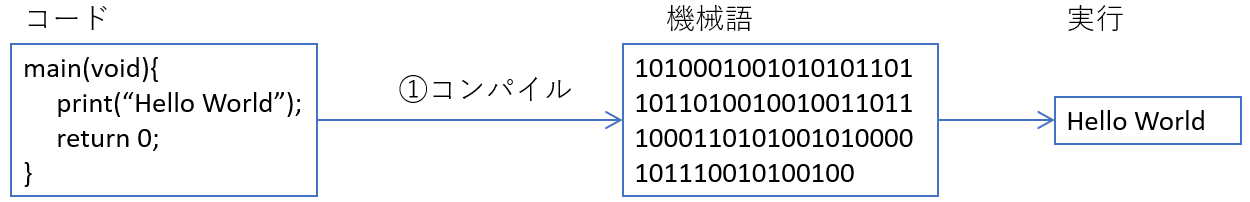
\includegraphics{././image/compile.png}

}

\caption{図1:コンパイルと機械語への変換}

\end{figure}

一方,インタプリタ型の言語では,プログラミング言語をコンパイルすることなく実行することができます.インタプリタ型の言語には\href{https://www.python.org/}{Python}や\href{https://www.ruby-lang.org/ja/}{Ruby},\href{https://www.php.net/}{PHP},\href{https://julialang.org/}{Julia}などがあります.コンパイルには通常時間がかかりますが,インタプリタ型言語ではコンパイルに時間をかけることなく,すぐにプログラムを実行することができるというメリットがあります.一方で,プログラムを実行し,完了するまでの時間はコンパイルを行うプログラミング言語よりも遅くなるというデメリットもあります.

Rはインタプリタ型の言語ですので,記述したプログラム(スクリプトとも呼びます)はすぐに実行されます.一方で,Rでの計算速度はインタプリタ型言語の中でもかなり遅い部類に入ります.ただし,Rは主にad
hocな(その場一回限りの)統計解析に用いられる言語です.1回限りであれば,それほど計算が早くなくても問題とはなりませんし,入力したプログラムがすぐに実行されるという性質も統計解析との相性がよいものです.コンピュータの性能も昔より遥かに高くなっており,R言語での計算が遅いと感じることは減ってきています.

\hypertarget{ux30aaux30d6ux30b8ux30a7ux30afux30c8ux3068ux306f}{%
\section{オブジェクトとは?}\label{ux30aaux30d6ux30b8ux30a7ux30afux30c8ux3068ux306f}}

Rは\textbf{オブジェクト指向(Object
oriented)}の言語である,とされています.この\textbf{「オブジェクト指向」}という言葉はプログラミング言語ではよく用いられるものですが,厳密な定義は複雑です.

この\textbf{オブジェクト}というのは,プログラミングで取り扱うものすべてを指す言葉です.プログラミングでは,\textbf{数値}や\textbf{文字}などを取り扱い,数値の演算を行ったり,文字に対して検索や置換,文字の追加などを行います.このとき,取り扱う数値や文字はオブジェクト,つまりプログラミングで用いる「もの」であるということになります.Rでは数値や文字の他に,\textbf{因子(factor)}や\textbf{論理値(booleanまたはlogical)},\textbf{関数(function)}などを取り扱います.これらのすべてがプログラミングで取り扱う「もの」,つまりオブジェクトです.

上で述べたように,プログラミングで用いるオブジェクトには数値,文字,因子,関数など,様々な種類のものがあります.数値も文字もプログラミングで扱う「もの」であることは共通していますが,数値と文字に対して同じ演算をしたい,ということは通常ありません.数値なら掛け算や割り算を行うことがあっても,文字に対して掛け算や割り算はしません.プログラミング言語も,数値なら数値の演算,文字なら文字の演算を行う必要があります.このように,数値なら数値の,文字なら文字の処理を行うために,オブジェクトには\textbf{「型(type)」}というものがあります.

\textbf{型と演算の関係}

\begin{Shaded}
\begin{Highlighting}[]
\DecValTok{1}\SpecialCharTok{*}\DecValTok{1} \CommentTok{\# 数値同士を掛け算することがあっても,}
\DocumentationTok{\#\# [1] 1}
\DecValTok{1}\SpecialCharTok{*}\StringTok{"dog"} \CommentTok{\# 数値と文字列を掛け算できてしまうと困る(エラーが出る)}
\DocumentationTok{\#\# Error in 1 * "dog": non{-}numeric argument to binary operator}
\end{Highlighting}
\end{Shaded}

\hypertarget{ux578btypeux3068ux306f}{%
\section{型(type)とは?}\label{ux578btypeux3068ux306f}}

\textbf{型(type)}とは,そのオブジェクトの種類を定めるためのラベルのようなものです.例えば,Rで数値を入力すると,Rは自動的にその数値がnumericであるという風に認識します.同様に,``(ダブルクオーテーション)で文字を囲うと,Rは自動的にその文字がcharacter(文字列型)であると認識します.Rはこの認識した型に従い,そのオブジェクトに対する演算を行います.

オブジェクトの型は\textbf{mode関数}で確認することができます.関数については後ほど詳しく説明します.

\textbf{typeof関数で型を確認する}

\begin{Shaded}
\begin{Highlighting}[]
\FunctionTok{mode}\NormalTok{(}\DecValTok{1}\NormalTok{) }\CommentTok{\# 1は数値}
\DocumentationTok{\#\# [1] "numeric"}
\FunctionTok{mode}\NormalTok{(}\StringTok{"Hello world"}\NormalTok{) }\CommentTok{\# "Hello world"は文字列}
\DocumentationTok{\#\# [1] "character"}
\FunctionTok{mode}\NormalTok{(}\StringTok{"1"}\NormalTok{) }\CommentTok{\# "1"は文字列}
\DocumentationTok{\#\# [1] "character"}
\end{Highlighting}
\end{Shaded}

上記のように,「1」の数字をmode()のカッコの中に入れると,numericが返ってきます.これは,1というオブジェクトの型がnumeric(数値)であることを示しています.同様に,ダブルクオーテーションで囲まれた''Hello
world''をmode()のカッコに入れると,characterが返ってきます.これは,``Hello
world''の型がcharacter(文字列)であることを意味しています.では,ダブルクオーテーションで囲まれた''1''がどうなるかというと,これはcharacter,つまり文字列であるということになります.

Rでは,このように「ダブルクオーテーションで囲まれている」というオブジェクトの状態を調べ,囲まれていればそのオブジェクトは文字列型であると判断します.同様に,オブジェクトが「数値でかつダブルクオーテーションに囲まれていない」場合には,そのオブジェクトが数値型であると判断します.このように,プログラム上でオブジェクトの型を特に指定していなくても,Rは自動的にそのオブジェクトの型を決定してくれます.このようなプログラムの性質を\textbf{「型推論」}と呼びます.

では,Rの代表的な型について,これから簡単に説明していきます.

\hypertarget{ux6587ux5b57ux5217character}{%
\subsection{文字列(character)}\label{ux6587ux5b57ux5217character}}

一般的なプログラミング言語で最も取り扱うことが多いオブジェクトは\textbf{文字列型(character)}です.文字列,つまり文章などを検索したり,一部を取り出したり,条件に合っているか確認したりすることはプログラミング利用の目的の一つとなります.

Rは統計学のプログラミング言語ですので,どちらかというと文字列よりは数値を取り扱うことが多いのですが,文字列を取り扱える仕組みを一通り備えています.

Rで文字列型のオブジェクトを作成するときには,``(ダブルクオーテーション)もしくは'(シングルクォーテーション)で文字を囲みます.ダブルクオーテーション・シングルクオーテーションのどちらを用いても文字列のオブジェクトを作成することはできます.

\textbf{文字列オブジェクトの例}

\begin{Shaded}
\begin{Highlighting}[]
\StringTok{"Hello world"} \CommentTok{\# ダブルクオーテーションで囲った場合}
\DocumentationTok{\#\# [1] "Hello world"}
\StringTok{\textquotesingle{}Hello R\textquotesingle{}} \CommentTok{\# シングルクオーテーションで囲った場合}
\DocumentationTok{\#\# [1] "Hello R"}
\end{Highlighting}
\end{Shaded}

では,ダブルクオーテーションとシングルクオーテーションの違いは何かというと,何も違いません.どちらを用いても問題ないのですが,Rではダブルクオーテーションを用いるのが一般的です.

\hypertarget{ux30a8ux30b9ux30b1ux30fcux30d7ux6587ux5b57ux30a8ux30b9ux30b1ux30fcux30d7ux30b7ux30fcux30b1ux30f3ux30b9}{%
\subsubsection{エスケープ文字(エスケープシーケンス)}\label{ux30a8ux30b9ux30b1ux30fcux30d7ux6587ux5b57ux30a8ux30b9ux30b1ux30fcux30d7ux30b7ux30fcux30b1ux30f3ux30b9}}

プログラミング言語によっては,ダブルクオーテーションとシングルクオーテーションで\textbf{エスケープ文字(エスケープシーケンス)}の取扱いに違いがある場合があります.エスケープシーケンスとは,バックスラッシュ(\,日本語キーボードでは¥)とアルファベットを組み合わせて,特定の意味を持たせる表現のことを指します.例えば,\textbackslash nは改行を,\textbackslash tはタブを示す記号です.RではC言語由来のエスケープシーケンスを利用できることになっています.以下にエスケープシーケンスの例を挙げます.

\begin{longtable}[]{@{}ll@{}}
\caption{表1:エスケープ文字の例}\tabularnewline
\toprule()
エスケープ文字 & エスケープ文字の意味 \\
\midrule()
\endfirsthead
\toprule()
エスケープ文字 & エスケープ文字の意味 \\
\midrule()
\endhead
\textbackslash a & アラート \\
\textbackslash b & バックスペース \\
\textbackslash f & ページ分割 \\
\textbackslash n & 改行 \\
\textbackslash r & キャリッジリターン \\
\textbackslash t & 水平タブ \\
\textbackslash v & 垂直タブ \\
\textbackslash\textbackslash{} & バックスラッシュ \\
\textbackslash\textquotesingle{} & シングルクオーテーション \\
\textbackslash" & ダブルクオーテーション \\
\bottomrule()
\end{longtable}

Rで表示しているときに必要となるエスケープ記号は,ダブルクオーテーションやシングルクオーテーションを用いるときのみです.ただし,Rのデータをテキストファイルなどに書き出すときには,エスケープ文字,特に\textbackslash n(改行)や\textbackslash t(タブ)を用いることがあります.データ書き出しの際のエスケープ文字に関しては,別の章で詳しく説明します.

エスケープシーケンスを変換した文字列を表示する場合には,writeLines関数を用います.

\begin{Shaded}
\begin{Highlighting}[]
\FunctionTok{writeLines}\NormalTok{(}\StringTok{"Hello world"}\NormalTok{)}
\end{Highlighting}
\end{Shaded}

\begin{verbatim}
Hello world
\end{verbatim}

\begin{Shaded}
\begin{Highlighting}[]
\FunctionTok{writeLines}\NormalTok{(}\StringTok{"Hello}\SpecialCharTok{\textbackslash{}n}\StringTok{world"}\NormalTok{) }\CommentTok{\# \textbackslash{}nは改行に変換}
\end{Highlighting}
\end{Shaded}

\begin{verbatim}
Hello
world
\end{verbatim}

\begin{Shaded}
\begin{Highlighting}[]
\FunctionTok{print}\NormalTok{(}\StringTok{"Hello}\SpecialCharTok{\textbackslash{}n}\StringTok{world"}\NormalTok{) }\CommentTok{\# print関数はエスケープシーケンスを変換しない}
\end{Highlighting}
\end{Shaded}

\begin{verbatim}
[1] "Hello\nworld"
\end{verbatim}

\hypertarget{ux6587ux5b57ux5217ux3092ux7d50ux5408ux3059ux308b}{%
\subsubsection{文字列を結合する}\label{ux6587ux5b57ux5217ux3092ux7d50ux5408ux3059ux308b}}

Rで文字列を用いるときに,文字列Aと文字列Bをくっつけたい,ということがあります.このようなときに用いるのが,\textbf{paste関数}です.paste関数はカッコの中に2つ以上の文字列をコンマでつないで入れると,文字列をスペースを挟んでつなぎ合わせてくれます.文字列の間にスペースが必要ない場合には,paste0関数を用います.

\textbf{文字列をつなぐpaste関数}

\begin{Shaded}
\begin{Highlighting}[]
\FunctionTok{paste}\NormalTok{(}\StringTok{"Hello"}\NormalTok{, }\StringTok{"world"}\NormalTok{)}
\DocumentationTok{\#\# [1] "Hello world"}
\FunctionTok{paste0}\NormalTok{(}\StringTok{"Hello"}\NormalTok{, }\StringTok{"R"}\NormalTok{)}
\DocumentationTok{\#\# [1] "HelloR"}
\end{Highlighting}
\end{Shaded}

文字列の取扱いに関しては,別の章で詳しく説明します.

\hypertarget{ux6570ux5024numeric}{%
\subsection{数値(numeric)}\label{ux6570ux5024numeric}}

Rは統計の言語ですので,数値データを取り扱う機会が特に多いです.グラフを記述したり,データを要約する場合にも主に取り扱うのは数値です.Rでは,数値は\textbf{numeric}という型を持ちます.

\hypertarget{ux6570ux5024ux578bux306edoubleux6d6eux52d5ux5c0fux6570ux70b9ux3068integerux6574ux6570}{%
\subsubsection{数値型のdouble(浮動小数点)とinteger(整数)}\label{ux6570ux5024ux578bux306edoubleux6d6eux52d5ux5c0fux6570ux70b9ux3068integerux6574ux6570}}

数値には更に詳細な型があります.詳細な型は\textbf{typeof関数}で調べることができます.Rでの数値は通常doubleという型を持ちます.

\begin{quote}
プログラミング言語の小数点を含む数値は,その精度(桁数)により,single(浮動小数点型),double(倍精度浮動小数点型)などの型を持ちます.このsingleはdoubleよりオブジェクトのファイルサイズが小さい代わりに,あまり大きい桁数の数値は取り扱えないという特徴があります.Rにはsingleという型はなく,doubleのみが使用されます.
\end{quote}

数値にはdouble以外に,integer(整数)という型もあります.Rで整数型の数値を利用する時には,数字の後ろにLをつけます.数値であっても,ダブルクオーテーションで囲うと文字列
(character)になります.

\textbf{double型とinteger型}

\begin{Shaded}
\begin{Highlighting}[]
\FunctionTok{mode}\NormalTok{(}\DecValTok{1}\NormalTok{) }\CommentTok{\# modeでの型はnumeric}
\end{Highlighting}
\end{Shaded}

\begin{verbatim}
[1] "numeric"
\end{verbatim}

\begin{Shaded}
\begin{Highlighting}[]
\FunctionTok{typeof}\NormalTok{(}\DecValTok{1}\NormalTok{) }\CommentTok{\# これはdouble}
\end{Highlighting}
\end{Shaded}

\begin{verbatim}
[1] "double"
\end{verbatim}

\begin{Shaded}
\begin{Highlighting}[]
\FunctionTok{typeof}\NormalTok{(1L) }\CommentTok{\# これはinteger}
\end{Highlighting}
\end{Shaded}

\begin{verbatim}
[1] "integer"
\end{verbatim}

\begin{Shaded}
\begin{Highlighting}[]
\FunctionTok{typeof}\NormalTok{(}\StringTok{"1"}\NormalTok{) }\CommentTok{\# これはcharacter}
\end{Highlighting}
\end{Shaded}

\begin{verbatim}
[1] "character"
\end{verbatim}

Rではintegerを取り扱う機会は非常に少なく,通常数値はdoubleとして取り扱います.

\hypertarget{ux30afux30e9ux30b9class}{%
\subsubsection{クラス(class)}\label{ux30afux30e9ux30b9class}}

Rではオブジェクトは型以外に,\textbf{クラス(class)}という性質を別に持っています.Rでの数値型は,numeric(数値)というクラスを持ちます.クラスの確認には\textbf{class関数}を用います.

\textbf{クラス,モードとtypeof関数}

\begin{Shaded}
\begin{Highlighting}[]
\FunctionTok{mode}\NormalTok{(}\DecValTok{1}\NormalTok{) }\CommentTok{\# 型はnumeric}
\end{Highlighting}
\end{Shaded}

\begin{verbatim}
[1] "numeric"
\end{verbatim}

\begin{Shaded}
\begin{Highlighting}[]
\FunctionTok{typeof}\NormalTok{(}\DecValTok{1}\NormalTok{) }\CommentTok{\# typeofだとdouble}
\end{Highlighting}
\end{Shaded}

\begin{verbatim}
[1] "double"
\end{verbatim}

\begin{Shaded}
\begin{Highlighting}[]
\FunctionTok{class}\NormalTok{(}\DecValTok{1}\NormalTok{) }\CommentTok{\# クラスはnumeric}
\end{Highlighting}
\end{Shaded}

\begin{verbatim}
[1] "numeric"
\end{verbatim}

\begin{quote}
Rのオブジェクトは型だけでなく,アトリビュート(Attribute)という性質を別に持っています.クラスはこのAttributeの一つです.オブジェクト指向プログラミングではクラスは非常に重要な意味を持ちますので,別の機会に詳しく説明します.
\end{quote}

\hypertarget{ux6f14ux7b97ux5b50operator}{%
\subsubsection{演算子(operator)}\label{ux6f14ux7b97ux5b50operator}}

数値を扱う際には,四則演算等の計算を行うことがあります.この四則演算を行うための記号のことを,\textbf{演算子}と呼びます.Rでは以下の四則演算子を利用できます.

\begin{longtable}[]{@{}ll@{}}
\caption{表2:Rで使える演算子}\tabularnewline
\toprule()
演算子 & 演算の種類 \\
\midrule()
\endfirsthead
\toprule()
演算子 & 演算の種類 \\
\midrule()
\endhead
+ & 足し算 \\
- & 引き算 \\
* & 掛け算 \\
/ & 割り算 \\
\%\% & 剰余(割り算の余り) \\
\%/\% & 整数の割り算 \\
\^{} & 累乗 \\
\bottomrule()
\end{longtable}

演算子それぞれの計算結果は以下のようになります.ほとんどの演算子はExcelなどで用いられているものと同じです.

\textbf{四則演算の例}

\begin{Shaded}
\begin{Highlighting}[]
\DecValTok{3}\SpecialCharTok{+}\DecValTok{2} \CommentTok{\# 足し算}
\end{Highlighting}
\end{Shaded}

\begin{verbatim}
[1] 5
\end{verbatim}

\begin{Shaded}
\begin{Highlighting}[]
\DecValTok{3{-}2} \CommentTok{\# 引き算}
\end{Highlighting}
\end{Shaded}

\begin{verbatim}
[1] 1
\end{verbatim}

\begin{Shaded}
\begin{Highlighting}[]
\DecValTok{3}\SpecialCharTok{*}\DecValTok{2} \CommentTok{\# 掛け算}
\end{Highlighting}
\end{Shaded}

\begin{verbatim}
[1] 6
\end{verbatim}

\begin{Shaded}
\begin{Highlighting}[]
\DecValTok{3}\SpecialCharTok{/}\DecValTok{2} \CommentTok{\# 割り算}
\end{Highlighting}
\end{Shaded}

\begin{verbatim}
[1] 1.5
\end{verbatim}

\begin{Shaded}
\begin{Highlighting}[]
\DecValTok{3}\SpecialCharTok{\%\%}\DecValTok{2} \CommentTok{\# 剰余(余り)}
\end{Highlighting}
\end{Shaded}

\begin{verbatim}
[1] 1
\end{verbatim}

\begin{Shaded}
\begin{Highlighting}[]
\DecValTok{3}\SpecialCharTok{\%/\%}\DecValTok{2} \CommentTok{\# 整数の割り算}
\end{Highlighting}
\end{Shaded}

\begin{verbatim}
[1] 1
\end{verbatim}

\begin{Shaded}
\begin{Highlighting}[]
\DecValTok{3}\SpecialCharTok{\^{}}\DecValTok{2} \CommentTok{\# 累乗}
\end{Highlighting}
\end{Shaded}

\begin{verbatim}
[1] 9
\end{verbatim}

\hypertarget{ux56e0ux5b50factor}{%
\subsection{因子(factor)}\label{ux56e0ux5b50factor}}

\textbf{因子(factor)}はR以外のプログラミング言語にはない型の一つです.因子とは,カテゴリを表すときに用いる型です.カテゴリとは,例えば男性/女性や,成人/未成年,喫煙者/非喫煙者などの,そのデータの性質を表す要素のことを指します.統計では,例えば男性と女性で分けて数値を集計する,といったシチュエーションがたくさんあります.このように,カテゴリごとの集計や統計を行いやすくするために準備されている型が因子です.因子は\textbf{factor関数}を用いて作成します.

\textbf{因子型(factor)}

\begin{Shaded}
\begin{Highlighting}[]
\FunctionTok{factor}\NormalTok{(}\StringTok{"male"}\NormalTok{) }\CommentTok{\# 男性を示す因子}
\end{Highlighting}
\end{Shaded}

\begin{verbatim}
[1] male
Levels: male
\end{verbatim}

\begin{Shaded}
\begin{Highlighting}[]
\FunctionTok{mode}\NormalTok{(}\FunctionTok{factor}\NormalTok{(}\StringTok{"male"}\NormalTok{)) }\CommentTok{\# 因子の型はfactor}
\end{Highlighting}
\end{Shaded}

\begin{verbatim}
[1] "numeric"
\end{verbatim}

\begin{quote}
因子には,レベル(Levels)というアトリビュートが付いています.因子はカテゴリを示すものですので,通常1つだけで用いることはありません(カテゴリが1つだけであれば,カテゴリ分けする必要がありません).因子については後ほど詳しく説明します.
\end{quote}

\hypertarget{ux8ad6ux7406ux578blogical}{%
\subsection{論理型(logical)}\label{ux8ad6ux7406ux578blogical}}

\textbf{論理型(logical)}は,\textbf{TRUE(真)}と\textbf{FALSE(偽)}からなる2値の型です.TRUEとFALSEはその名の通り,その関係が正しいか,間違っているかを意味するものです.論理型はそのまま使用することもありますが,プログラミングでは\textbf{比較演算子}と共に用いることが多い型です.

\hypertarget{ux6bd4ux8f03ux6f14ux7b97ux5b50}{%
\subsubsection{比較演算子}\label{ux6bd4ux8f03ux6f14ux7b97ux5b50}}

\textbf{比較演算子}とは,演算子の右と左を比較して,その関係が正しい(TRUE)のか,間違っているのか(FALSE)を返す演算子です.比較演算子の例を以下に示します.

\begin{longtable}[]{@{}ll@{}}
\caption{表3:Rで使える比較演算子}\tabularnewline
\toprule()
比較演算子 & 比較演算子の意味 \\
\midrule()
\endfirsthead
\toprule()
比較演算子 & 比較演算子の意味 \\
\midrule()
\endhead
== & 等しい \\
!= & 等しくない \\
\textless{} & 小なり \\
\textless= & 小なりイコール \\
\textgreater{} & 大なり \\
\textgreater= & 大なりイコール \\
\& & かつ \\
\&\& & かつ \\
\textbar{} & または \\
\textbar\textbar{} & または \\
\bottomrule()
\end{longtable}

\&と\textbar は比較演算子同士を結びつけるための演算子(論理演算子)です.\&と\&\&,\textbar と\textbar\textbar の違いについては,後ほど説明します.

比較演算子を用いた演算の例を以下に示します.比較演算子や論理型は主に\textbf{条件分岐}で用います.

\textbf{比較演算子}

\begin{Shaded}
\begin{Highlighting}[]
\DecValTok{1} \SpecialCharTok{==} \DecValTok{1} \CommentTok{\# 等しいのでTRUE}
\end{Highlighting}
\end{Shaded}

\begin{verbatim}
[1] TRUE
\end{verbatim}

\begin{Shaded}
\begin{Highlighting}[]
\DecValTok{1} \SpecialCharTok{==} \DecValTok{2} \CommentTok{\# 等しくないのでFALSE}
\end{Highlighting}
\end{Shaded}

\begin{verbatim}
[1] FALSE
\end{verbatim}

\begin{Shaded}
\begin{Highlighting}[]
\DecValTok{1} \SpecialCharTok{!=} \DecValTok{1} \CommentTok{\# 等しいのでFALSE}
\end{Highlighting}
\end{Shaded}

\begin{verbatim}
[1] FALSE
\end{verbatim}

\begin{Shaded}
\begin{Highlighting}[]
\DecValTok{1} \SpecialCharTok{!=} \DecValTok{2} \CommentTok{\# 等しくないのでTRUE}
\end{Highlighting}
\end{Shaded}

\begin{verbatim}
[1] TRUE
\end{verbatim}

\begin{Shaded}
\begin{Highlighting}[]
\DecValTok{1} \SpecialCharTok{\textless{}} \DecValTok{2} \CommentTok{\# 2は1より小さいのでTRUE}
\end{Highlighting}
\end{Shaded}

\begin{verbatim}
[1] TRUE
\end{verbatim}

\begin{Shaded}
\begin{Highlighting}[]
\DecValTok{1} \SpecialCharTok{\textless{}} \DecValTok{1} \CommentTok{\# 1は1より小さくないのでFALSE}
\end{Highlighting}
\end{Shaded}

\begin{verbatim}
[1] FALSE
\end{verbatim}

\begin{Shaded}
\begin{Highlighting}[]
\DecValTok{1} \SpecialCharTok{\textless{}=} \DecValTok{2} \CommentTok{\# 2は1より小さいのでTRUE}
\end{Highlighting}
\end{Shaded}

\begin{verbatim}
[1] TRUE
\end{verbatim}

\begin{Shaded}
\begin{Highlighting}[]
\DecValTok{1} \SpecialCharTok{\textless{}=} \DecValTok{1} \CommentTok{\# 1は1に等しいのでTURE}
\end{Highlighting}
\end{Shaded}

\begin{verbatim}
[1] TRUE
\end{verbatim}

\begin{Shaded}
\begin{Highlighting}[]
\DecValTok{3} \SpecialCharTok{\textgreater{}} \DecValTok{2} \CommentTok{\# 3は2より大きいのでTRUE}
\end{Highlighting}
\end{Shaded}

\begin{verbatim}
[1] TRUE
\end{verbatim}

\begin{Shaded}
\begin{Highlighting}[]
\DecValTok{2} \SpecialCharTok{\textgreater{}} \DecValTok{2} \CommentTok{\# 2は2より大きくないのでFALSE}
\end{Highlighting}
\end{Shaded}

\begin{verbatim}
[1] FALSE
\end{verbatim}

\begin{Shaded}
\begin{Highlighting}[]
\DecValTok{3} \SpecialCharTok{\textgreater{}=} \DecValTok{2} \CommentTok{\# 3は2より大きいのでTRUE}
\end{Highlighting}
\end{Shaded}

\begin{verbatim}
[1] TRUE
\end{verbatim}

\begin{Shaded}
\begin{Highlighting}[]
\DecValTok{2} \SpecialCharTok{\textgreater{}=} \DecValTok{2} \CommentTok{\# 2は2と等しいのでTRUE}
\end{Highlighting}
\end{Shaded}

\begin{verbatim}
[1] TRUE
\end{verbatim}

\begin{Shaded}
\begin{Highlighting}[]
\DecValTok{1} \SpecialCharTok{==} \DecValTok{1} \SpecialCharTok{\&} \DecValTok{2} \SpecialCharTok{==} \DecValTok{2} \CommentTok{\# TRUEかつTRUEなのでTRUE}
\end{Highlighting}
\end{Shaded}

\begin{verbatim}
[1] TRUE
\end{verbatim}

\begin{Shaded}
\begin{Highlighting}[]
\DecValTok{1} \SpecialCharTok{==} \DecValTok{1} \SpecialCharTok{\&} \DecValTok{2} \SpecialCharTok{==} \DecValTok{3} \CommentTok{\# TRUEかつFALSEなのでFALSE}
\end{Highlighting}
\end{Shaded}

\begin{verbatim}
[1] FALSE
\end{verbatim}

\begin{Shaded}
\begin{Highlighting}[]
\DecValTok{1} \SpecialCharTok{==} \DecValTok{1} \SpecialCharTok{|} \DecValTok{2} \SpecialCharTok{==} \DecValTok{2} \CommentTok{\# TRUEまたはTRUEなのでTRUE}
\end{Highlighting}
\end{Shaded}

\begin{verbatim}
[1] TRUE
\end{verbatim}

\begin{Shaded}
\begin{Highlighting}[]
\DecValTok{1} \SpecialCharTok{==} \DecValTok{1} \SpecialCharTok{|} \DecValTok{2} \SpecialCharTok{==} \DecValTok{3} \CommentTok{\# TRUEまたはFALSEなのでTRUE}
\end{Highlighting}
\end{Shaded}

\begin{verbatim}
[1] TRUE
\end{verbatim}

\hypertarget{ux6f14ux7b97ux5b50ux306eux512aux5148ux9806ux4f4d}{%
\subsubsection{演算子の優先順位}\label{ux6f14ux7b97ux5b50ux306eux512aux5148ux9806ux4f4d}}

数値の計算で掛け算・割り算を足し算・引き算より前に計算するように,演算子の優先順位,計算する順番は決まっています.概ね通常の計算と同じですが,以下のような順序で演算子は計算されます.

\begin{enumerate}
\def\labelenumi{\arabic{enumi}.}
\tightlist
\item
  カッコでくくられている計算
\item
  累乗(\^{})
\item
  剰余・整数の割り算(\%\%・\%/\%)
\item
  掛け算・割り算(*・/)
\item
  足し算・引き算(+・-)
\item
  比較演算子(==,!=,\textless,\textless=,\textgreater,\textgreater=)
\item
  論理演算子(\&,\textbar)
\end{enumerate}

計算式は長くなることが多く,演算子の計算順を間違う場合も多いため,優先する計算は積極的にカッコで囲むとよいでしょう.

\textbf{演算子の計算順序}

\begin{Shaded}
\begin{Highlighting}[]
\NormalTok{(}\DecValTok{2} \SpecialCharTok{+} \DecValTok{1}\NormalTok{) }\SpecialCharTok{/} \DecValTok{3} \CommentTok{\# カッコ内は最優先}
\end{Highlighting}
\end{Shaded}

\begin{verbatim}
[1] 1
\end{verbatim}

\begin{Shaded}
\begin{Highlighting}[]
\DecValTok{2} \SpecialCharTok{\^{}} \DecValTok{3} \SpecialCharTok{\%\%} \DecValTok{5} \CommentTok{\# 累乗は剰余より先に計算(8/5の余り)}
\end{Highlighting}
\end{Shaded}

\begin{verbatim}
[1] 3
\end{verbatim}

\begin{Shaded}
\begin{Highlighting}[]
\DecValTok{3} \SpecialCharTok{/} \DecValTok{3} \SpecialCharTok{\%\%} \DecValTok{2} \CommentTok{\# 剰余は割り算より先に計算(3/1を計算)}
\end{Highlighting}
\end{Shaded}

\begin{verbatim}
[1] 3
\end{verbatim}

\begin{Shaded}
\begin{Highlighting}[]
\DecValTok{3} \SpecialCharTok{/} \DecValTok{3} \SpecialCharTok{+} \DecValTok{1} \CommentTok{\# 割り算は足し算より先に計算}
\end{Highlighting}
\end{Shaded}

\begin{verbatim}
[1] 2
\end{verbatim}

\begin{Shaded}
\begin{Highlighting}[]
\DecValTok{3} \SpecialCharTok{+} \DecValTok{3} \SpecialCharTok{\textgreater{}} \DecValTok{5} \CommentTok{\# 比較演算子は足し算より後に計算}
\end{Highlighting}
\end{Shaded}

\begin{verbatim}
[1] TRUE
\end{verbatim}

\begin{Shaded}
\begin{Highlighting}[]
\DecValTok{5} \SpecialCharTok{\textgreater{}} \DecValTok{1} \SpecialCharTok{\&} \DecValTok{6} \SpecialCharTok{\textgreater{}} \DecValTok{2} \CommentTok{\# 論理演算子は最後に計算}
\end{Highlighting}
\end{Shaded}

\begin{verbatim}
[1] TRUE
\end{verbatim}

\hypertarget{ux305dux306eux4ed6ux306eux30afux30e9ux30b9}{%
\subsection{その他のクラス}\label{ux305dux306eux4ed6ux306eux30afux30e9ux30b9}}

以上の4つ(文字列,数値,因子,論理型)がRでの基本的な型になります.しかし,Rにはこの4つ以外の型を持つオブジェクトも存在します.

\hypertarget{ux6b20ux640dux5024ux306aux3069}{%
\subsubsection{欠損値など}\label{ux6b20ux640dux5024ux306aux3069}}

データ分析では欠損値や,計算結果が表示できないもの,計算結果が無限大になるものなど,データとしてうまく取り扱えない値が生じることがよくあります.このような場合に対応するため,Rは欠損値,計算できない値,無限大にそれぞれNA,NaN,Infという型が設定されています.Rでは中身が何もないオブジェクト,NULLというものを作成することもできます.

\textbf{欠損値,非数,無限大}

\begin{Shaded}
\begin{Highlighting}[]
\ConstantTok{NA} \CommentTok{\# 欠損値(Not Available)}
\end{Highlighting}
\end{Shaded}

\begin{verbatim}
[1] NA
\end{verbatim}

\begin{Shaded}
\begin{Highlighting}[]
\DecValTok{0}\SpecialCharTok{/}\DecValTok{0} \CommentTok{\# 非数(NaN,Not A Number)}
\end{Highlighting}
\end{Shaded}

\begin{verbatim}
[1] NaN
\end{verbatim}

\begin{Shaded}
\begin{Highlighting}[]
\DecValTok{1}\SpecialCharTok{/}\DecValTok{0} \CommentTok{\# 無限大(Inf)}
\end{Highlighting}
\end{Shaded}

\begin{verbatim}
[1] Inf
\end{verbatim}

\begin{Shaded}
\begin{Highlighting}[]
\DecValTok{10000}\SpecialCharTok{\^{}}\DecValTok{1000000} \CommentTok{\# 大きすぎて取り扱えない数値もInfになる}
\end{Highlighting}
\end{Shaded}

\begin{verbatim}
[1] Inf
\end{verbatim}

\begin{Shaded}
\begin{Highlighting}[]
\ConstantTok{NULL} \CommentTok{\# 中身がないオブジェクト(NULL)}
\end{Highlighting}
\end{Shaded}

\begin{verbatim}
NULL
\end{verbatim}

\hypertarget{ux8907ux7d20ux6570complex}{%
\subsubsection{複素数(complex)}\label{ux8907ux7d20ux6570complex}}

Rでは複素数(整数+虚数)を取り扱うこともできます.複素数を表すときには,数値の後にiを入力します.

\textbf{複素数の作成と演算}

\begin{Shaded}
\begin{Highlighting}[]
\DecValTok{1} \SpecialCharTok{+}\NormalTok{ 1i }\CommentTok{\# 複素数}
\end{Highlighting}
\end{Shaded}

\begin{verbatim}
[1] 1+1i
\end{verbatim}

\begin{Shaded}
\begin{Highlighting}[]
\FunctionTok{mode}\NormalTok{(}\DecValTok{1} \SpecialCharTok{+}\NormalTok{ 1i) }\CommentTok{\# 複素数の型はcomplex}
\end{Highlighting}
\end{Shaded}

\begin{verbatim}
[1] "complex"
\end{verbatim}

\begin{Shaded}
\begin{Highlighting}[]
\NormalTok{(}\DecValTok{1} \SpecialCharTok{+}\NormalTok{ 1i) }\SpecialCharTok{+}\NormalTok{ (}\DecValTok{3} \SpecialCharTok{+}\NormalTok{ 3i) }\CommentTok{\# 複素数同士の足し算}
\end{Highlighting}
\end{Shaded}

\begin{verbatim}
[1] 4+4i
\end{verbatim}

\hypertarget{ux65e5ux6642ux306eux30afux30e9ux30b9dateposixctposixltdifftime}{%
\subsubsection{日時のクラス(Date,POSIXct,POSIXlt,difftime)}\label{ux65e5ux6642ux306eux30afux30e9ux30b9dateposixctposixltdifftime}}

日付は数値や文字列とは異なる性質を持ちます.統計では日付や時間を演算に用いることもあります.Rでは日付はDateというクラスを持ちます.また,日時のデータはPOSIXctやPOSIXltというクラスに属します.

DateやPOSIXct,POSIXltは引き算などの演算に用いることができます.日時の差はdulationsというクラスを持ちます.

Date,POSIXct,POSIXlt,dulationはいずれもクラスで,データの型としてはdouble,つまり数値型のデータとして取り扱われます.

\textbf{日時のクラスと型}

\begin{Shaded}
\begin{Highlighting}[]
\FunctionTok{Sys.Date}\NormalTok{() }\CommentTok{\# 現在の日付を表示する関数}
\end{Highlighting}
\end{Shaded}

\begin{verbatim}
[1] "2023-10-31"
\end{verbatim}

\begin{Shaded}
\begin{Highlighting}[]
\FunctionTok{class}\NormalTok{(}\FunctionTok{Sys.Date}\NormalTok{()) }\CommentTok{\# 日付のクラスはDate}
\end{Highlighting}
\end{Shaded}

\begin{verbatim}
[1] "Date"
\end{verbatim}

\begin{Shaded}
\begin{Highlighting}[]
\FunctionTok{typeof}\NormalTok{(}\FunctionTok{Sys.Date}\NormalTok{()) }\CommentTok{\# 日付の型はdouble}
\end{Highlighting}
\end{Shaded}

\begin{verbatim}
[1] "double"
\end{verbatim}

\begin{Shaded}
\begin{Highlighting}[]
\FunctionTok{Sys.time}\NormalTok{() }\CommentTok{\# 現在の日時を表示する関数}
\end{Highlighting}
\end{Shaded}

\begin{verbatim}
[1] "2023-10-31 14:56:04 JST"
\end{verbatim}

\begin{Shaded}
\begin{Highlighting}[]
\FunctionTok{class}\NormalTok{(}\FunctionTok{Sys.time}\NormalTok{()) }\CommentTok{\# 日時のクラスはPOSIXctとPOSIXlt}
\end{Highlighting}
\end{Shaded}

\begin{verbatim}
[1] "POSIXct" "POSIXt" 
\end{verbatim}

\begin{Shaded}
\begin{Highlighting}[]
\FunctionTok{typeof}\NormalTok{(}\FunctionTok{Sys.time}\NormalTok{()) }\CommentTok{\# 日時の型はdouble}
\end{Highlighting}
\end{Shaded}

\begin{verbatim}
[1] "double"
\end{verbatim}

\begin{Shaded}
\begin{Highlighting}[]
\FunctionTok{Sys.Date}\NormalTok{() }\SpecialCharTok{{-}} \FunctionTok{as.Date}\NormalTok{(}\StringTok{"2023{-}01{-}01"}\NormalTok{) }\CommentTok{\# 2022/1/1から今日までの日数}
\end{Highlighting}
\end{Shaded}

\begin{verbatim}
Time difference of 303 days
\end{verbatim}

\begin{Shaded}
\begin{Highlighting}[]
\FunctionTok{class}\NormalTok{(}\FunctionTok{Sys.Date}\NormalTok{() }\SpecialCharTok{{-}} \FunctionTok{as.Date}\NormalTok{(}\StringTok{"2023{-}01{-}01"}\NormalTok{)) }\CommentTok{\# 日時の差のクラスはdifftime}
\end{Highlighting}
\end{Shaded}

\begin{verbatim}
[1] "difftime"
\end{verbatim}

\begin{quote}
Rには,これらの型の他に,S3,S4,R5(Reference
Class),R6というデータ型が存在します.これらのデータ型は関数などの計算結果に用いられていることがあります.これらのオブジェクトについては,クラスとオブジェクト指向と関連していますので,クラスの詳しい説明に合わせて解説します.
\end{quote}

\hypertarget{ux5909ux6570ux3068ux5b9aux6570}{%
\section{変数と定数}\label{ux5909ux6570ux3068ux5b9aux6570}}

\hypertarget{ux5909ux6570}{%
\subsection{変数}\label{ux5909ux6570}}

ココまでは,数値や文字列などの,単純なオブジェクトについて説明してきました.単純なオブジェクトはプログラミングの要素として重要です.しかし,オブジェクトを毎回作成し直すのは面倒です.オブジェクトを作ったら,それを一時的に保管しておいて,後から演算に使える方が便利です.

電卓では,このような「一時的に結果を記録する」方法として,メモリー機能があります.Excelなどでは,計算結果をセルに記録しておくこともあるでしょう.プログラミング言語にも,計算結果を一時的に保管しておくものが準備されています.この「計算結果を一時的に保管しておくもの」のことを,プログラミング言語では\textbf{変数}と呼びます.

変数には名前がついています.名前付きの箱の中にオブジェクトを入れているようなものが変数です.下の図では,変数「dog」にオブジェクト「犬」を入れています.「犬」を取り出して使いたいときには,変数である「dog」を持ってくればよい,ということになります.

\begin{figure}

{\centering 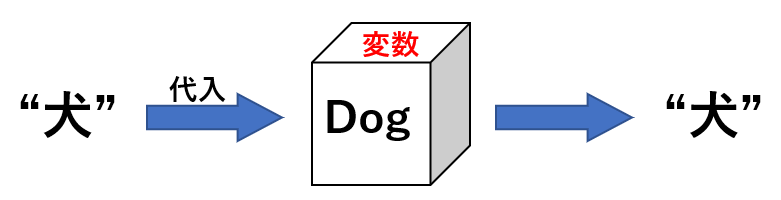
\includegraphics{././image/variable_image.png}

}

\caption{図2:変数のイメージ}

\end{figure}

Rで変数を作成する場合には,変数名に「\textless-」の記号でオブジェクトを\textbf{代入}します.

\textbf{変数への代入}

\begin{Shaded}
\begin{Highlighting}[]
\NormalTok{dog }\OtherTok{\textless{}{-}} \StringTok{"inu"} \CommentTok{\# dogという変数に"inu"という文字列を代入する}
\NormalTok{number }\OtherTok{\textless{}{-}} \DecValTok{1} \CommentTok{\# numberという変数に,1という数値を代入する}
\NormalTok{dog }\CommentTok{\# 変数dogには"inu"が入っている}
\end{Highlighting}
\end{Shaded}

\begin{verbatim}
[1] "inu"
\end{verbatim}

\begin{Shaded}
\begin{Highlighting}[]
\NormalTok{number }\CommentTok{\# 変数numberには1が入っている}
\end{Highlighting}
\end{Shaded}

\begin{verbatim}
[1] 1
\end{verbatim}

変数には型があり,代入したオブジェクトと同じ型を持つことになります.また,変数はそのまま演算に用いることができます.

\textbf{変数の型}

\begin{Shaded}
\begin{Highlighting}[]
\FunctionTok{mode}\NormalTok{(dog) }\CommentTok{\# dogの中身は文字列}
\end{Highlighting}
\end{Shaded}

\begin{verbatim}
[1] "character"
\end{verbatim}

\begin{Shaded}
\begin{Highlighting}[]
\FunctionTok{mode}\NormalTok{(number) }\CommentTok{\# numberの中身は数値}
\end{Highlighting}
\end{Shaded}

\begin{verbatim}
[1] "numeric"
\end{verbatim}

\begin{Shaded}
\begin{Highlighting}[]
\FunctionTok{paste}\NormalTok{(dog, }\StringTok{"walk"}\NormalTok{) }\CommentTok{\# dogの中身と"walk"をつなぐ}
\end{Highlighting}
\end{Shaded}

\begin{verbatim}
[1] "inu walk"
\end{verbatim}

\begin{Shaded}
\begin{Highlighting}[]
\NormalTok{number }\SpecialCharTok{+} \DecValTok{5} \CommentTok{\# numberの中身に5を足す}
\end{Highlighting}
\end{Shaded}

\begin{verbatim}
[1] 6
\end{verbatim}

\begin{Shaded}
\begin{Highlighting}[]
\NormalTok{dog }\SpecialCharTok{+} \DecValTok{1} \CommentTok{\# dogの中身は文字列なので,足し算はできない}
\end{Highlighting}
\end{Shaded}

\begin{verbatim}
Error in dog + 1: non-numeric argument to binary operator
\end{verbatim}

変数への代入は,「=」や「-\textgreater」の演算子によっても行うことができます.ただし,これらを代入に用いると,プログラムを理解しにくくなるため,Rでは「\textless-」を用いることが推奨されています.

\textbf{=や-\textgreater による代入}

\begin{Shaded}
\begin{Highlighting}[]
\NormalTok{dog }\OtherTok{=} \StringTok{"犬"} \CommentTok{\# イコールも代入に使うことができる}
\DecValTok{2} \OtherTok{{-}\textgreater{}}\NormalTok{ number }\CommentTok{\# {-}\textgreater{}も代入に使える(方向は\textless{}{-}と逆になる)}
\NormalTok{dog}
\end{Highlighting}
\end{Shaded}

\begin{verbatim}
[1] "犬"
\end{verbatim}

\begin{Shaded}
\begin{Highlighting}[]
\NormalTok{number}
\end{Highlighting}
\end{Shaded}

\begin{verbatim}
[1] 2
\end{verbatim}

\hypertarget{ux5b9aux6570}{%
\subsection{定数}\label{ux5b9aux6570}}

変数のうち,一度代入したら中身を変えられないもののことを\textbf{定数}と呼びます.他のプログラミング言語では定数を設定できるものが多いのですが,Rには定数を設定する方法はありません.変数の中身はいつでも置き換えできます.変数を置き換えると,置き換えたオブジェクトの型で変数の型も置き換わります.

\textbf{変数の置き換え}

\begin{Shaded}
\begin{Highlighting}[]
\NormalTok{dog }\OtherTok{\textless{}{-}} \StringTok{"inu"} \CommentTok{\# 変数に文字列を代入}
\FunctionTok{mode}\NormalTok{(dog) }\CommentTok{\# 型は文字列になる}
\end{Highlighting}
\end{Shaded}

\begin{verbatim}
[1] "character"
\end{verbatim}

\begin{Shaded}
\begin{Highlighting}[]
\NormalTok{dog }\OtherTok{\textless{}{-}} \DecValTok{1} \CommentTok{\# 変数に数値を入れ直す}
\FunctionTok{mode}\NormalTok{(dog) }\CommentTok{\# 変数の型は数値になる}
\end{Highlighting}
\end{Shaded}

\begin{verbatim}
[1] "numeric"
\end{verbatim}

\begin{quote}
多くのプログラミング言語では,このように変数の型が変化するのを抑える仕組み(型宣言)を持っています.型宣言が必要な言語では,変数は厳密に型のチェックを受けます(静的型付け).Rはこのような仕組みがなく,代入されたオブジェクトに従って型が決まり,型チェックされることなくプログラムが実行されます.このような言語のことを動的型付けと呼びます.
\end{quote}

プログラム中で変数の型が変わると,バグの原因となります.Rでは,プログラムを書いているうちに変数の型が変化していて,計算結果がおかしくなる,ということがたびたび起きます.変数の型を確認しながらプログラミングした方がよいでしょう.

定数とは少し異なりますが,Rでは代入なしに使える変数もあります.例えば,円周率のπは「pi」という変数名で始めから登録されています.このような変数にも別のオブジェクトを代入することはできますが,後々混乱する原因となるため避けたほうがよいでしょう.

また,統計を試すことができるデータが代入されている変数(データセット)もたくさん設定されています.データセットについては,後ほど詳しく説明します.

\textbf{あらかじめ設定されている変数}

\begin{Shaded}
\begin{Highlighting}[]
\NormalTok{pi }\CommentTok{\# 円周率}
\end{Highlighting}
\end{Shaded}

\begin{verbatim}
[1] 3.141593
\end{verbatim}

\begin{Shaded}
\begin{Highlighting}[]
\NormalTok{letters }\CommentTok{\# アルファベット(小文字)}
\end{Highlighting}
\end{Shaded}

\begin{verbatim}
 [1] "a" "b" "c" "d" "e" "f" "g" "h" "i" "j" "k" "l" "m" "n" "o" "p" "q" "r" "s"
[20] "t" "u" "v" "w" "x" "y" "z"
\end{verbatim}

\begin{Shaded}
\begin{Highlighting}[]
\NormalTok{LETTERS }\CommentTok{\# アルファベット(大文字)}
\end{Highlighting}
\end{Shaded}

\begin{verbatim}
 [1] "A" "B" "C" "D" "E" "F" "G" "H" "I" "J" "K" "L" "M" "N" "O" "P" "Q" "R" "S"
[20] "T" "U" "V" "W" "X" "Y" "Z"
\end{verbatim}

\begin{Shaded}
\begin{Highlighting}[]
\NormalTok{month.abb }\CommentTok{\# 月(短縮表記)}
\end{Highlighting}
\end{Shaded}

\begin{verbatim}
 [1] "Jan" "Feb" "Mar" "Apr" "May" "Jun" "Jul" "Aug" "Sep" "Oct" "Nov" "Dec"
\end{verbatim}

\begin{Shaded}
\begin{Highlighting}[]
\NormalTok{month.name }\CommentTok{\# 月}
\end{Highlighting}
\end{Shaded}

\begin{verbatim}
 [1] "January"   "February"  "March"     "April"     "May"       "June"     
 [7] "July"      "August"    "September" "October"   "November"  "December" 
\end{verbatim}

\begin{Shaded}
\begin{Highlighting}[]
\NormalTok{pi }\OtherTok{\textless{}{-}} \DecValTok{3} \CommentTok{\# piに3を代入する}
\NormalTok{pi }\CommentTok{\# piは3になってしまう}
\end{Highlighting}
\end{Shaded}

\begin{verbatim}
[1] 3
\end{verbatim}

\hypertarget{ux5024ux6e21ux3057ux3068ux53c2ux7167ux6e21ux3057}{%
\subsection{値渡しと参照渡し}\label{ux5024ux6e21ux3057ux3068ux53c2ux7167ux6e21ux3057}}

Rでは,変数への代入が行われるたびに,その変数に対するメモリのアドレスを新規に作成し直す,という特徴があるため,他の言語で理解が必要となる値渡しと参照渡しの問題がほとんど起きません.

\begin{Shaded}
\begin{Highlighting}[]
\NormalTok{x }\OtherTok{\textless{}{-}} \DecValTok{1} \CommentTok{\# xに1を代入}
\NormalTok{y }\OtherTok{\textless{}{-}}\NormalTok{ x }\CommentTok{\# yにxを代入(yとxはメモリを共有)}
\NormalTok{x }\OtherTok{\textless{}{-}} \DecValTok{2} \CommentTok{\# xに2を代入(xのメモリのアドレスが変わる)}
\NormalTok{x }\CommentTok{\# xは新しいアドレスを参照(2が返ってくる)}
\end{Highlighting}
\end{Shaded}

\begin{verbatim}
[1] 2
\end{verbatim}

\begin{Shaded}
\begin{Highlighting}[]
\NormalTok{y }\CommentTok{\# yは古いアドレスを参照(1が返ってくる)}
\end{Highlighting}
\end{Shaded}

\begin{verbatim}
[1] 1
\end{verbatim}

\begin{quote}
上のコードでは,参照渡しであれば,xの値が2になった場合,xとメモリを共有しているyも2になります.Rでは,代入時にメモリのアドレスが変更になるため(値渡し),参照渡しが起こることは基本的にありません.この特徴はプログラミング初心者には優しいのですが,変数の変更のたびにメモリ上にオブジェクトを新規作成するため,Rの実行速度が遅い原因になります.
\end{quote}

\hypertarget{ux4fbfux5229ux306aux30aaux30d6ux30b8ux30a7ux30afux30c8}{%
\section{便利なオブジェクト}\label{ux4fbfux5229ux306aux30aaux30d6ux30b8ux30a7ux30afux30c8}}

ここまでは,オブジェクトが一つだけの場合のデータ型や,変数について見てきました.しかし,統計で取り扱うのは,通常たくさんの数値や記録です.数値や記録がたくさんある場合には,数値や記録を一つづつ別々に取り扱うのは非効率です.多くのプログラミング言語では,このようなたくさんの数値や記録を取り扱う専用のオブジェクトを備えています.Rでは,たくさんの記録を取り扱うオブジェクトとして,\textbf{ベクター(vector)},\textbf{リスト(list)},\textbf{データフレーム(data.frame)},\textbf{行列(matrix)}の4つが用いられます.この4つについて簡単に説明します.それぞれのオブジェクトについてはさらに別章で詳しく説明します.

\hypertarget{ux30d9ux30afux30bfux30fcvector}{%
\subsection{ベクター(vector)}\label{ux30d9ux30afux30bfux30fcvector}}

Rで最も基本的なオブジェクトは,ベクター(vector)です.ベクターは同じ型を持つオブジェクトの集まりで,1次元の,つまり縦横の構造がないデータとして取り扱われます.ベクターは\textbf{c関数}(cはcombine,「結合する」の意味)で作成することができます.

ベクターは同じ型を持つデータの集まりです.ですので,ベクターの要素に文字列が交じると,自動的にすべての要素が文字列になる,という特徴があります.

\textbf{ベクターの作成}

\begin{Shaded}
\begin{Highlighting}[]
\NormalTok{vec\_n }\OtherTok{\textless{}{-}} \FunctionTok{c}\NormalTok{(}\DecValTok{1}\NormalTok{, }\DecValTok{2}\NormalTok{, }\DecValTok{3}\NormalTok{, }\DecValTok{4}\NormalTok{) }\CommentTok{\# 数値のベクター}
\NormalTok{vec\_c }\OtherTok{\textless{}{-}} \FunctionTok{c}\NormalTok{(}\StringTok{"dog"}\NormalTok{, }\StringTok{"cat"}\NormalTok{, }\StringTok{"pig"}\NormalTok{, }\StringTok{"horse"}\NormalTok{) }\CommentTok{\# 文字列のベクター}
\NormalTok{vec\_temp }\OtherTok{\textless{}{-}} \FunctionTok{c}\NormalTok{(}\DecValTok{1}\NormalTok{, }\DecValTok{2}\NormalTok{, }\DecValTok{3}\NormalTok{, }\StringTok{"dog"}\NormalTok{) }\CommentTok{\# 文字列が交じると文字列のベクターになる}

\NormalTok{vec\_n}
\end{Highlighting}
\end{Shaded}

\begin{verbatim}
[1] 1 2 3 4
\end{verbatim}

\begin{Shaded}
\begin{Highlighting}[]
\NormalTok{vec\_c}
\end{Highlighting}
\end{Shaded}

\begin{verbatim}
[1] "dog"   "cat"   "pig"   "horse"
\end{verbatim}

\begin{Shaded}
\begin{Highlighting}[]
\NormalTok{vec\_temp}
\end{Highlighting}
\end{Shaded}

\begin{verbatim}
[1] "1"   "2"   "3"   "dog"
\end{verbatim}

Rでは数値1つや文字列1つの要素も,ベクターとして取り扱われます.ですので,Rのオブジェクトの最小単位はベクターとなります.要素が1つであれば,c関数でつなぎ合わせる必要はありません.

\begin{Shaded}
\begin{Highlighting}[]
\DecValTok{1} \CommentTok{\# 数字1つでもベクター}
\end{Highlighting}
\end{Shaded}

\begin{verbatim}
[1] 1
\end{verbatim}

\begin{Shaded}
\begin{Highlighting}[]
\StringTok{"Hello world"} \CommentTok{\# 文字列1つでもベクター}
\end{Highlighting}
\end{Shaded}

\begin{verbatim}
[1] "Hello world"
\end{verbatim}

\begin{quote}
vectorはベクトルと表記されることもあります.この文書では,Rのオブジェクトをベクター,方向と大きさを持つ量のことをベクトルと表記することとします.
\end{quote}

\hypertarget{ux30d9ux30afux30bfux30fcux306bux8981ux7d20ux3092ux8ffdux52a0ux3059ux308b}{%
\subsubsection{ベクターに要素を追加する}\label{ux30d9ux30afux30bfux30fcux306bux8981ux7d20ux3092ux8ffdux52a0ux3059ux308b}}

ベクターに要素を追加するために,append関数というものが用意されています.しかし,上記のc関数でもベクターに要素を追加することができます.

append関数では位置を特定して要素を追加することができますが,位置を特定して要素を追加することはまれです.

\textbf{ベクターに要素を追加する}

\begin{Shaded}
\begin{Highlighting}[]
\FunctionTok{append}\NormalTok{(vec\_n, }\DecValTok{5}\NormalTok{) }\CommentTok{\# 上の数値ベクターに5を追加}
\end{Highlighting}
\end{Shaded}

\begin{verbatim}
[1] 1 2 3 4 5
\end{verbatim}

\begin{Shaded}
\begin{Highlighting}[]
\FunctionTok{c}\NormalTok{(vec\_n, }\DecValTok{5}\NormalTok{) }\CommentTok{\# 上と同じ}
\end{Highlighting}
\end{Shaded}

\begin{verbatim}
[1] 1 2 3 4 5
\end{verbatim}

\hypertarget{ux30d9ux30afux30bfux30fcux306eux8981ux7d20ux3092ux53d6ux308aux51faux3059}{%
\subsubsection{ベクターの要素を取り出す}\label{ux30d9ux30afux30bfux30fcux306eux8981ux7d20ux3092ux53d6ux308aux51faux3059}}

ベクターの要素を取り出すときには,\textbf{インデックス}というものを用います.インデックスとは,ベクターなどの複数の値を取り扱うオブジェクトにおいて,値のある位置を示す数値のことです.インデックスはベクターの変数の後に,四角カッコ({[}{]})に数値を入れることで指定することができます.Rではインデックスは1から始まります.

\begin{quote}
多くのプログラミング言語では,インデックスは0から始まります.インデックスが1から始まるプログラミング言語はまれです.
\end{quote}

\begin{figure}

{\centering 
\includegraphics{././image/vector_index.png}

}

\caption{図3:ベクターとインデックス}

\end{figure}

\textbf{ベクターの要素をインデックスで取り出す}

\begin{Shaded}
\begin{Highlighting}[]
\NormalTok{vec }\OtherTok{\textless{}{-}} \FunctionTok{c}\NormalTok{(}\DecValTok{4}\NormalTok{, }\DecValTok{3}\NormalTok{, }\DecValTok{2}\NormalTok{, }\DecValTok{1}\NormalTok{) }\CommentTok{\# 数値のベクターを作成する}
\NormalTok{vec[}\DecValTok{1}\NormalTok{] }\CommentTok{\# インデックス1には4が入っている}
\end{Highlighting}
\end{Shaded}

\begin{verbatim}
[1] 4
\end{verbatim}

\begin{Shaded}
\begin{Highlighting}[]
\NormalTok{vec[}\DecValTok{3}\NormalTok{] }\CommentTok{\# インデックス3には2が入っている}
\end{Highlighting}
\end{Shaded}

\begin{verbatim}
[1] 2
\end{verbatim}

\hypertarget{ux30d9ux30afux30bfux30fcux306eux8981ux7d20ux306eux7f6eux304dux63dbux3048}{%
\subsubsection{ベクターの要素の置き換え}\label{ux30d9ux30afux30bfux30fcux306eux8981ux7d20ux306eux7f6eux304dux63dbux3048}}

ベクターの要素を置き換えるときには,置き換えたいベクターのインデックスを指定し,代入します.この時,数値のベクターの要素を文字列に置き換えると,ベクター全体が文字列に置き換わるので注意して下さい.

\textbf{ベクターの要素を置き換える}

\begin{Shaded}
\begin{Highlighting}[]
\NormalTok{vec }\CommentTok{\# 数値のベクター}
\end{Highlighting}
\end{Shaded}

\begin{verbatim}
[1] 4 3 2 1
\end{verbatim}

\begin{Shaded}
\begin{Highlighting}[]
\NormalTok{vec[}\DecValTok{3}\NormalTok{] }\OtherTok{\textless{}{-}} \DecValTok{5} \CommentTok{\# インデックス3の数値を5に置き換える}
\NormalTok{vec }\CommentTok{\# 3番めが2から5に置き換わる}
\end{Highlighting}
\end{Shaded}

\begin{verbatim}
[1] 4 3 5 1
\end{verbatim}

\begin{Shaded}
\begin{Highlighting}[]
\NormalTok{vec[}\DecValTok{4}\NormalTok{] }\OtherTok{\textless{}{-}} \StringTok{"dog"} \CommentTok{\# インデックス4の数値を"dog"(文字列)に置き換える}
\NormalTok{vec }\CommentTok{\# ベクターはすべて文字列になる}
\end{Highlighting}
\end{Shaded}

\begin{verbatim}
[1] "4"   "3"   "5"   "dog"
\end{verbatim}

\hypertarget{ux30d9ux30afux30bfux30fcux306eux8981ux7d20ux3092ux53d6ux308aux9664ux304f}{%
\subsubsection{ベクターの要素を取り除く}\label{ux30d9ux30afux30bfux30fcux306eux8981ux7d20ux3092ux53d6ux308aux9664ux304f}}

ベクターの要素を取り除くときには,\textbf{ベクターのインデックスをマイナス}で指定します.マイナスのインデックスで指定した要素は取り除かれ,ベクターの長さが短くなります.

\textbf{ベクターの要素を取り除く}

\begin{Shaded}
\begin{Highlighting}[]
\NormalTok{vec}
\end{Highlighting}
\end{Shaded}

\begin{verbatim}
[1] "4"   "3"   "5"   "dog"
\end{verbatim}

\begin{Shaded}
\begin{Highlighting}[]
\NormalTok{vec[}\SpecialCharTok{{-}}\DecValTok{3}\NormalTok{] }\CommentTok{\# インデックス3の要素(5)を取り除く}
\end{Highlighting}
\end{Shaded}

\begin{verbatim}
[1] "4"   "3"   "dog"
\end{verbatim}

\hypertarget{ux30d9ux30afux30bfux30fcux306eux6f14ux7b97}{%
\subsubsection{ベクターの演算}\label{ux30d9ux30afux30bfux30fcux306eux6f14ux7b97}}

ベクターは,そのまま演算に用いることができます.数値のベクターに数値を足せば,ベクターのすべての要素に数値が足されます.文字列のベクターにpaste関数で文字を継ぎ足せば,すべての要素に文字が継ぎ足されます.

\textbf{ベクターを演算に用いる}

\begin{Shaded}
\begin{Highlighting}[]
\NormalTok{vec\_n }\CommentTok{\# 数値のベクター}
\end{Highlighting}
\end{Shaded}

\begin{verbatim}
[1] 1 2 3 4
\end{verbatim}

\begin{Shaded}
\begin{Highlighting}[]
\NormalTok{vec\_n }\SpecialCharTok{+} \DecValTok{5} \CommentTok{\# 数値のベクターに5を足すと,すべての要素に5が足される}
\end{Highlighting}
\end{Shaded}

\begin{verbatim}
[1] 6 7 8 9
\end{verbatim}

\begin{Shaded}
\begin{Highlighting}[]
\NormalTok{vec\_c }\CommentTok{\# 文字のベクター}
\end{Highlighting}
\end{Shaded}

\begin{verbatim}
[1] "dog"   "cat"   "pig"   "horse"
\end{verbatim}

\begin{Shaded}
\begin{Highlighting}[]
\FunctionTok{paste}\NormalTok{(vec\_c, }\StringTok{"is animal."}\NormalTok{) }\CommentTok{\# 文字のベクターにpaste関数で文字をつなぎ合わせる}
\end{Highlighting}
\end{Shaded}

\begin{verbatim}
[1] "dog is animal."   "cat is animal."   "pig is animal."   "horse is animal."
\end{verbatim}

ベクターについては別の章でさらに詳しく説明します.

\hypertarget{ux30eaux30b9ux30c8list}{%
\subsection{リスト(list)}\label{ux30eaux30b9ux30c8list}}

統計の計算をしていると,複数の計算結果をまとめて取り扱いたい,という場合があります.ベクターは1次元のオブジェクトで,かつすべての要素のデータ型が同じですので,ベクターでは型や長さの違う,様々な結果を一度に取り扱うことはできません.このような,型の違うデータを一度に取り扱うときに用いられるのが,\textbf{リスト(list)}と呼ばれるオブジェクトです.リストは,様々なオブジェクトをまとめて一つにしたようなデータ構造を持ちます.リストを作成するときには,\textbf{list関数}を用います.

\textbf{リスト(list)の作成}

\begin{Shaded}
\begin{Highlighting}[]
\NormalTok{vec1 }\OtherTok{\textless{}{-}} \FunctionTok{c}\NormalTok{(}\DecValTok{1}\NormalTok{, }\DecValTok{2}\NormalTok{, }\DecValTok{3}\NormalTok{, }\DecValTok{4}\NormalTok{) }\CommentTok{\# 数値のベクター}
\NormalTok{vec2 }\OtherTok{\textless{}{-}} \FunctionTok{c}\NormalTok{(}\StringTok{"dog"}\NormalTok{, }\StringTok{"cat"}\NormalTok{, }\StringTok{"pig"}\NormalTok{, }\StringTok{"horse"}\NormalTok{) }\CommentTok{\# 文字列のベクター}
\NormalTok{num }\OtherTok{\textless{}{-}} \DecValTok{10} \CommentTok{\# 数値}
\NormalTok{char\_temp }\OtherTok{\textless{}{-}} \StringTok{"Hello world"} \CommentTok{\# 文字列}

\NormalTok{list\_temp }\OtherTok{\textless{}{-}} \FunctionTok{list}\NormalTok{(vec1, vec2, num, char\_temp) }\CommentTok{\# 色々な要素をリストにまとめる}
\NormalTok{list\_temp }\CommentTok{\# まとめたリストを表示}
\end{Highlighting}
\end{Shaded}

\begin{verbatim}
[[1]]
[1] 1 2 3 4

[[2]]
[1] "dog"   "cat"   "pig"   "horse"

[[3]]
[1] 10

[[4]]
[1] "Hello world"
\end{verbatim}

\hypertarget{ux30eaux30b9ux30c8ux306eux8981ux7d20ux3092ux53d6ux308aux51faux3059}{%
\subsubsection{リストの要素を取り出す}\label{ux30eaux30b9ux30c8ux306eux8981ux7d20ux3092ux53d6ux308aux51faux3059}}

リストの要素を取り出す場合には,ベクターと同様にインデックスを用います.ただし,リストのインデックスは多層化,ネストされているため,呼び出しはやや複雑です.リストの要素を取り出すときには,四角カッコを2重にして用います(\textbf{{[}{[}{]}{]}}).{[}{[}1{]}{]}で呼び出すと,リストの1番目の要素を呼び出すことになります.ベクターと同様に\textbf{{[}1{]}で呼び出すと,リストの1番目の要素を,リストとして呼び出す}ことになり,要素までたどり着けなくなります.

\textbf{リストの要素を取り出す}

\begin{Shaded}
\begin{Highlighting}[]
\NormalTok{list\_temp[[}\DecValTok{1}\NormalTok{]] }\CommentTok{\# リストの1番目の要素を取り出す}
\end{Highlighting}
\end{Shaded}

\begin{verbatim}
[1] 1 2 3 4
\end{verbatim}

\begin{Shaded}
\begin{Highlighting}[]
\NormalTok{list\_temp[[}\DecValTok{2}\NormalTok{]] }\CommentTok{\# 2番目の要素を取り出す}
\end{Highlighting}
\end{Shaded}

\begin{verbatim}
[1] "dog"   "cat"   "pig"   "horse"
\end{verbatim}

\begin{Shaded}
\begin{Highlighting}[]
\NormalTok{list\_temp[}\DecValTok{1}\NormalTok{] }\CommentTok{\# リストの1番目の要素を,リストとして取り出す}
\end{Highlighting}
\end{Shaded}

\begin{verbatim}
[[1]]
[1] 1 2 3 4
\end{verbatim}

\begin{Shaded}
\begin{Highlighting}[]
\NormalTok{list\_temp[[}\DecValTok{1}\NormalTok{]][}\DecValTok{1}\NormalTok{] }\CommentTok{\# リストの1番目の要素(ベクター)の,1番目の要素を取り出す}
\end{Highlighting}
\end{Shaded}

\begin{verbatim}
[1] 1
\end{verbatim}

リストについても,別の章で詳しく説明します.

\hypertarget{ux30c7ux30fcux30bfux30d5ux30ecux30fcux30e0data.frame}{%
\subsection{データフレーム(data.frame)}\label{ux30c7ux30fcux30bfux30d5ux30ecux30fcux30e0data.frame}}

\textbf{データフレーム(data.frame)}はExcelの表のように,行と列を持ち,長方形の形に整形された表型のオブジェクトです.データフレームはExcelの表のように取り扱うことができです.

データフレームは\textbf{縦方向(列)に同じデータ型}を持つ,ベクターの集合になっています.データフレームは横方向(行)には異なる型を持つことができますが,縦方向(列)は必ず同じ型を持つ必要があります.ベクターと同じように,\textbf{数値の列の1つのデータを文字列に置き換えると,その列のデータが全て文字列に変換される}という特徴があります.

\begin{quote}
データフレームは同じ長さの縦ベクターをリストにして,横に並べたものです.ですので,縦(列)はベクターとして同じ型を持ちます.データフレームはリストでもあるので,リストと同じように取り扱うこともできます.
\end{quote}

データフレームは\textbf{data.frame関数}を用いて作ることができます.データフレームを作成するときには,\textbf{「列名」=「列の要素」}というものをカッコの中に書きます.

\textbf{データフレームの作成}

\begin{Shaded}
\begin{Highlighting}[]
\NormalTok{d }\OtherTok{\textless{}{-}} \FunctionTok{data.frame}\NormalTok{( }\CommentTok{\# データフレームを作成する(各列を同じ長さにする)}
  \AttributeTok{number =} \FunctionTok{c}\NormalTok{(}\DecValTok{1}\NormalTok{, }\DecValTok{2}\NormalTok{, }\DecValTok{3}\NormalTok{, }\DecValTok{4}\NormalTok{), }\CommentTok{\# 1列目は数値}
  \AttributeTok{animal =} \FunctionTok{c}\NormalTok{(}\StringTok{"dog"}\NormalTok{, }\StringTok{"cat"}\NormalTok{, }\StringTok{"pig"}\NormalTok{, }\StringTok{"horse"}\NormalTok{), }\CommentTok{\# 2列目と3列目は動物と果物}
  \AttributeTok{fruits =} \FunctionTok{c}\NormalTok{(}\StringTok{"apple"}\NormalTok{, }\StringTok{"orange"}\NormalTok{, }\StringTok{"banana"}\NormalTok{, }\StringTok{"grape"}\NormalTok{)}
\NormalTok{)}

\NormalTok{d }\CommentTok{\# データフレームの表示}
\end{Highlighting}
\end{Shaded}

\begin{verbatim}
  number animal fruits
1      1    dog  apple
2      2    cat orange
3      3    pig banana
4      4  horse  grape
\end{verbatim}

\hypertarget{ux30c7ux30fcux30bfux30d5ux30ecux30fcux30e0ux306eux6b21ux5143dimensionux3068ux884cux6570ux5217ux6570}{%
\subsubsection{データフレームの次元(dimension)と行数・列数}\label{ux30c7ux30fcux30bfux30d5ux30ecux30fcux30e0ux306eux6b21ux5143dimensionux3068ux884cux6570ux5217ux6570}}

データフレームには,\textbf{次元(dimension)}という性質(アトリビュート,attribute)があります.この次元とは,行の数,列の数のことです.次元を取得する時には,\textbf{dim関数}を用います.また,行の数,列の数はそれぞれ\textbf{nrow関数},\textbf{ncol関数}で取得することができます.

\textbf{データフレームの次元を取得する}

\begin{Shaded}
\begin{Highlighting}[]
\FunctionTok{dim}\NormalTok{(d) }\CommentTok{\# 次元の取得(前が行の数,後ろが列の数)}
\end{Highlighting}
\end{Shaded}

\begin{verbatim}
[1] 4 3
\end{verbatim}

\begin{Shaded}
\begin{Highlighting}[]
\FunctionTok{nrow}\NormalTok{(d) }\CommentTok{\# 行の数}
\end{Highlighting}
\end{Shaded}

\begin{verbatim}
[1] 4
\end{verbatim}

\begin{Shaded}
\begin{Highlighting}[]
\FunctionTok{ncol}\NormalTok{(d) }\CommentTok{\# 列の数}
\end{Highlighting}
\end{Shaded}

\begin{verbatim}
[1] 3
\end{verbatim}

\hypertarget{ux30c7ux30fcux30bfux30d5ux30ecux30fcux30e0ux306eux30a4ux30f3ux30c7ux30c3ux30afux30b9}{%
\subsubsection{データフレームのインデックス}\label{ux30c7ux30fcux30bfux30d5ux30ecux30fcux30e0ux306eux30a4ux30f3ux30c7ux30c3ux30afux30b9}}

データフレームにも,インデックスで要素を取り出すことができます.データフレームのインデックスは,\textbf{{[}行,
列{]}}という形で指定します.行も列も,1行目・1列目のインデックスが1となります.

データフレームでは,行だけ,列だけをインデックスとして指定することもできます.\textbf{行だけをインデックスとして指定した時({[}行,
{]}の形で指定)には,その行がデータフレームとして取り出されます}.一方,列だけを指定した時({[},
列{]}の形で指定)には,その列がベクターとして取り出されます.データフレームを行と列で取り出した場合には異なるものが取り出されるので,特にデータフレームの行を取り出す際には注意が必要です.

\textbf{データフレームの要素を取り出す}

\begin{Shaded}
\begin{Highlighting}[]
\NormalTok{d[}\DecValTok{2}\NormalTok{, }\DecValTok{3}\NormalTok{] }\CommentTok{\# 2行3列目のデータを取り出す}
\end{Highlighting}
\end{Shaded}

\begin{verbatim}
[1] "orange"
\end{verbatim}

\begin{Shaded}
\begin{Highlighting}[]
\NormalTok{d[}\DecValTok{2}\NormalTok{, ] }\CommentTok{\# 2行目を取り出す(データフレーム)}
\end{Highlighting}
\end{Shaded}

\begin{verbatim}
  number animal fruits
2      2    cat orange
\end{verbatim}

\begin{Shaded}
\begin{Highlighting}[]
\NormalTok{d[, }\DecValTok{3}\NormalTok{] }\CommentTok{\# 3列目を取り出す(ベクター)}
\end{Highlighting}
\end{Shaded}

\begin{verbatim}
[1] "apple"  "orange" "banana" "grape" 
\end{verbatim}

データフレームの列は,列の名前を用いても取り出すことができます.列を取り出すときには,\textbf{\$(ドルマーク)に列名}を繋げて記述します.

\textbf{列を列名で呼び出す}

\begin{Shaded}
\begin{Highlighting}[]
\NormalTok{d}\SpecialCharTok{$}\NormalTok{number }\CommentTok{\# 1列目の列名はnumber}
\end{Highlighting}
\end{Shaded}

\begin{verbatim}
[1] 1 2 3 4
\end{verbatim}

\begin{Shaded}
\begin{Highlighting}[]
\NormalTok{d}\SpecialCharTok{$}\NormalTok{animal }\CommentTok{\# 2列目の列名はanimal}
\end{Highlighting}
\end{Shaded}

\begin{verbatim}
[1] "dog"   "cat"   "pig"   "horse"
\end{verbatim}

\begin{Shaded}
\begin{Highlighting}[]
\NormalTok{d}\SpecialCharTok{$}\NormalTok{fruits }\CommentTok{\# 3列目の列名はfruits}
\end{Highlighting}
\end{Shaded}

\begin{verbatim}
[1] "apple"  "orange" "banana" "grape" 
\end{verbatim}

\hypertarget{ux30c7ux30fcux30bfux30d5ux30ecux30fcux30e0ux306eux8981ux7d20ux306eux7f6eux304dux63dbux3048}{%
\subsubsection{データフレームの要素の置き換え}\label{ux30c7ux30fcux30bfux30d5ux30ecux30fcux30e0ux306eux8981ux7d20ux306eux7f6eux304dux63dbux3048}}

データフレームの要素の置き換えは,ベクターと同じように,置き換えたい場所のインデックスを指定して,値を代入する形で行います.この時,その置き換える列の型と代入するデータの型が異なると,列の型がすべて置き換わることがあるので注意が必要です.

\textbf{データフレームの要素を置き換える}

\begin{Shaded}
\begin{Highlighting}[]
\NormalTok{d[}\DecValTok{2}\NormalTok{, }\DecValTok{3}\NormalTok{] }\OtherTok{\textless{}{-}} \StringTok{"peach"} \CommentTok{\# 2行3列目の要素をpeachに置き換える}
\NormalTok{d }\CommentTok{\# 2行3列目がpeachに置き換わる}
\end{Highlighting}
\end{Shaded}

\begin{verbatim}
  number animal fruits
1      1    dog  apple
2      2    cat  peach
3      3    pig banana
4      4  horse  grape
\end{verbatim}

\begin{Shaded}
\begin{Highlighting}[]
\NormalTok{d[}\DecValTok{2}\NormalTok{, }\DecValTok{1}\NormalTok{] }\OtherTok{\textless{}{-}} \StringTok{"tomato"} \CommentTok{\# 2行1列目をtomato(文字列)に置き換える}
\NormalTok{d }\CommentTok{\# 2行1列目がtomatoに置き換わる}
\end{Highlighting}
\end{Shaded}

\begin{verbatim}
  number animal fruits
1      1    dog  apple
2 tomato    cat  peach
3      3    pig banana
4      4  horse  grape
\end{verbatim}

\begin{Shaded}
\begin{Highlighting}[]
\FunctionTok{mode}\NormalTok{(d[, }\DecValTok{1}\NormalTok{]) }\CommentTok{\# 1列目が文字列に置き換わる}
\end{Highlighting}
\end{Shaded}

\begin{verbatim}
[1] "character"
\end{verbatim}

\hypertarget{ux30c7ux30fcux30bfux30d5ux30ecux30fcux30e0ux306eux884cux5217ux306eux524aux9664}{%
\subsubsection{データフレームの行・列の削除}\label{ux30c7ux30fcux30bfux30d5ux30ecux30fcux30e0ux306eux884cux5217ux306eux524aux9664}}

データフレームの行や列を削除するには,ベクターと同じように,インデックスをマイナスで与えます.インデックスをマイナスにすることで,そのインデックスの行・列を取り除くことができます.ただし,データフレームの1つの要素だけを削除することはできません(指定した行・列がまるごと削除されます).1つの要素だけを取り除く場合には,その要素のインデックスに対してNAを代入するとよいでしょう.

\textbf{データフレームの行・列を削除する}

\begin{Shaded}
\begin{Highlighting}[]
\NormalTok{d }\CommentTok{\# 元々のデータフレームは4行3列}
\end{Highlighting}
\end{Shaded}

\begin{verbatim}
  number animal fruits
1      1    dog  apple
2 tomato    cat  peach
3      3    pig banana
4      4  horse  grape
\end{verbatim}

\begin{Shaded}
\begin{Highlighting}[]
\NormalTok{d[}\SpecialCharTok{{-}}\DecValTok{1}\NormalTok{, ] }\CommentTok{\# 1行目を削除}
\end{Highlighting}
\end{Shaded}

\begin{verbatim}
  number animal fruits
2 tomato    cat  peach
3      3    pig banana
4      4  horse  grape
\end{verbatim}

\begin{Shaded}
\begin{Highlighting}[]
\NormalTok{d[, }\SpecialCharTok{{-}}\DecValTok{1}\NormalTok{] }\CommentTok{\# 1列目を削除}
\end{Highlighting}
\end{Shaded}

\begin{verbatim}
  animal fruits
1    dog  apple
2    cat  peach
3    pig banana
4  horse  grape
\end{verbatim}

\begin{Shaded}
\begin{Highlighting}[]
\NormalTok{d[}\SpecialCharTok{{-}}\DecValTok{2}\NormalTok{, }\SpecialCharTok{{-}}\DecValTok{3}\NormalTok{] }\CommentTok{\# 2列目と3列目を削除}
\end{Highlighting}
\end{Shaded}

\begin{verbatim}
  number animal
1      1    dog
3      3    pig
4      4  horse
\end{verbatim}

\begin{Shaded}
\begin{Highlighting}[]
\NormalTok{d[}\DecValTok{2}\NormalTok{, }\DecValTok{3}\NormalTok{] }\OtherTok{\textless{}{-}} \ConstantTok{NA} \CommentTok{\# 1要素だけを取り除くときは,NAを代入する}
\end{Highlighting}
\end{Shaded}

\hypertarget{ux884cux5217matrix}{%
\subsection{行列(matrix)}\label{ux884cux5217matrix}}

行列(matrix)は,線形代数(高校数学での行列計算)に用いるものです.行列は基本的には一つの型の要素からなる,行と列のあるオブジェクトです.行列はデータフレームとよく似ていますが,データフレームが列方向のベクターのリストであるのに対し,行列は次元(dimension)を持つベクターに近いものとなります.

Rで行列を作成するときには,matrix関数を用います.matrix関数では,カッコの中に,ベクター,行数,列数を指定する数値を与えます.

\textbf{行列を作成する}

\begin{Shaded}
\begin{Highlighting}[]
\CommentTok{\# 2行3列の行列}
\NormalTok{mat }\OtherTok{\textless{}{-}} \FunctionTok{matrix}\NormalTok{(}\FunctionTok{c}\NormalTok{(}\DecValTok{1}\NormalTok{,}\DecValTok{2}\NormalTok{,}\DecValTok{3}\NormalTok{,}\DecValTok{4}\NormalTok{,}\DecValTok{5}\NormalTok{,}\DecValTok{6}\NormalTok{), }\AttributeTok{nrow=}\DecValTok{2}\NormalTok{, }\AttributeTok{ncol=}\DecValTok{3}\NormalTok{) }\CommentTok{\# nrowは行数,ncolは列数}
\NormalTok{mat}
\end{Highlighting}
\end{Shaded}

\begin{verbatim}
     [,1] [,2] [,3]
[1,]    1    3    5
[2,]    2    4    6
\end{verbatim}

\hypertarget{ux884cux5217ux306eux6b21ux5143ux3068ux30a4ux30f3ux30c7ux30c3ux30afux30b9}{%
\subsubsection{行列の次元とインデックス}\label{ux884cux5217ux306eux6b21ux5143ux3068ux30a4ux30f3ux30c7ux30c3ux30afux30b9}}

行列の次元とインデックスに関しては,データフレームとほぼ同じです.行列の列にも名前をつけることができます.従って,列を取り出すときに列名を利用することもできます.取り出したものはいずれもベクターになります.要素・行・列の削除もデータフレームと同じ方法で行います.

\textbf{行列の要素の取り出し}

\begin{Shaded}
\begin{Highlighting}[]
\NormalTok{mat[}\DecValTok{1}\NormalTok{, }\DecValTok{1}\NormalTok{] }\CommentTok{\# 1行1列目の要素}
\end{Highlighting}
\end{Shaded}

\begin{verbatim}
[1] 1
\end{verbatim}

\begin{Shaded}
\begin{Highlighting}[]
\NormalTok{mat[}\DecValTok{1}\NormalTok{, ] }\CommentTok{\# 1行目の要素(ベクター)}
\end{Highlighting}
\end{Shaded}

\begin{verbatim}
[1] 1 3 5
\end{verbatim}

\begin{Shaded}
\begin{Highlighting}[]
\NormalTok{mat[, }\DecValTok{1}\NormalTok{] }\CommentTok{\# 1列目の要素(ベクター)}
\end{Highlighting}
\end{Shaded}

\begin{verbatim}
[1] 1 2
\end{verbatim}

\begin{Shaded}
\begin{Highlighting}[]
\FunctionTok{dim}\NormalTok{(mat) }\CommentTok{\# matのdimensionを表示}
\end{Highlighting}
\end{Shaded}

\begin{verbatim}
[1] 2 3
\end{verbatim}

\begin{Shaded}
\begin{Highlighting}[]
\FunctionTok{nrow}\NormalTok{(mat) }\CommentTok{\# matの行数を表示}
\end{Highlighting}
\end{Shaded}

\begin{verbatim}
[1] 2
\end{verbatim}

\begin{Shaded}
\begin{Highlighting}[]
\FunctionTok{ncol}\NormalTok{(mat) }\CommentTok{\# matの列数を表示}
\end{Highlighting}
\end{Shaded}

\begin{verbatim}
[1] 3
\end{verbatim}

\hypertarget{ux884cux5217ux306eux6f14ux7b97}{%
\subsubsection{行列の演算}\label{ux884cux5217ux306eux6f14ux7b97}}

データフレームとは異なり,数値の行列は演算に用いることができます.行列(線形代数)の計算のために,行列積,外積,クロネッカー積に対応する演算子が準備されています.

\begin{longtable}[]{@{}ll@{}}
\caption{表4:Rで使える行列の演算子}\tabularnewline
\toprule()
行列の演算子 & 演算子の意味 \\
\midrule()
\endfirsthead
\toprule()
行列の演算子 & 演算子の意味 \\
\midrule()
\endhead
\%*\% & 行列の積 \\
\%o\% & 外積 \\
\%x\% & クロネッカー積 \\
\bottomrule()
\end{longtable}

\textbf{行列の演算}

\begin{Shaded}
\begin{Highlighting}[]
\NormalTok{mat2 }\OtherTok{\textless{}{-}} \FunctionTok{matrix}\NormalTok{(}\FunctionTok{c}\NormalTok{(}\DecValTok{1}\NormalTok{, }\DecValTok{2}\NormalTok{, }\DecValTok{3}\NormalTok{, }\DecValTok{4}\NormalTok{, }\DecValTok{5}\NormalTok{, }\DecValTok{6}\NormalTok{), }\AttributeTok{nrow=}\DecValTok{3}\NormalTok{, }\AttributeTok{ncol=}\DecValTok{2}\NormalTok{)}

\NormalTok{mat }\SpecialCharTok{\%*\%}\NormalTok{ mat2 }\CommentTok{\# 行列の積}
\end{Highlighting}
\end{Shaded}

\begin{verbatim}
     [,1] [,2]
[1,]   22   49
[2,]   28   64
\end{verbatim}

\begin{Shaded}
\begin{Highlighting}[]
\NormalTok{mat }\SpecialCharTok{\%o\%}\NormalTok{ mat2 }\CommentTok{\# 外積}
\end{Highlighting}
\end{Shaded}

\begin{verbatim}
, , 1, 1

     [,1] [,2] [,3]
[1,]    1    3    5
[2,]    2    4    6

, , 2, 1

     [,1] [,2] [,3]
[1,]    2    6   10
[2,]    4    8   12

, , 3, 1

     [,1] [,2] [,3]
[1,]    3    9   15
[2,]    6   12   18

, , 1, 2

     [,1] [,2] [,3]
[1,]    4   12   20
[2,]    8   16   24

, , 2, 2

     [,1] [,2] [,3]
[1,]    5   15   25
[2,]   10   20   30

, , 3, 2

     [,1] [,2] [,3]
[1,]    6   18   30
[2,]   12   24   36
\end{verbatim}

\begin{Shaded}
\begin{Highlighting}[]
\NormalTok{mat }\SpecialCharTok{\%x\%}\NormalTok{ mat2 }\CommentTok{\# クロネッカー積}
\end{Highlighting}
\end{Shaded}

\begin{verbatim}
     [,1] [,2] [,3] [,4] [,5] [,6]
[1,]    1    4    3   12    5   20
[2,]    2    5    6   15   10   25
[3,]    3    6    9   18   15   30
[4,]    2    8    4   16    6   24
[5,]    4   10    8   20   12   30
[6,]    6   12   12   24   18   36
\end{verbatim}

\hypertarget{ux6b21ux5143ux4ee5ux4e0aux306eux30aaux30d6ux30b8ux30a7ux30afux30c8array}{%
\subsubsection{3次元以上のオブジェクト:array}\label{ux6b21ux5143ux4ee5ux4e0aux306eux30aaux30d6ux30b8ux30a7ux30afux30c8array}}

行列はベクターに次元を2つ(行と列)与えたものですが,3次元以上の次元を与えることもできます.このような3次元以上のデータを取り扱う場合には,arrayというオブジェクトを使用します.arrayはarray関数で作成することができ,各次元の数(行数,列数に当たるもの)をベクターで与えます.統計やデータ解析で3次元以上のデータを取り扱うことはまれです.

\textbf{arrayを作成する}

\begin{Shaded}
\begin{Highlighting}[]
\FunctionTok{array}\NormalTok{(}\FunctionTok{c}\NormalTok{(}\DecValTok{1}\NormalTok{, }\DecValTok{2}\NormalTok{, }\DecValTok{3}\NormalTok{, }\DecValTok{4}\NormalTok{, }\DecValTok{5}\NormalTok{, }\DecValTok{6}\NormalTok{, }\DecValTok{7}\NormalTok{, }\DecValTok{8}\NormalTok{), }\AttributeTok{dim =} \FunctionTok{c}\NormalTok{(}\DecValTok{2}\NormalTok{, }\DecValTok{2}\NormalTok{, }\DecValTok{2}\NormalTok{))}
\end{Highlighting}
\end{Shaded}

\begin{verbatim}
, , 1

     [,1] [,2]
[1,]    1    3
[2,]    2    4

, , 2

     [,1] [,2]
[1,]    5    7
[2,]    6    8
\end{verbatim}

\hypertarget{ux305dux306eux4ed6ux306eux30aaux30d6ux30b8ux30a7ux30afux30c8}{%
\subsection{その他のオブジェクト}\label{ux305dux306eux4ed6ux306eux30aaux30d6ux30b8ux30a7ux30afux30c8}}

Rに基本的に備わっているオブジェクトとして,ベクター,リスト,データフレーム,行列の他に,\textbf{時系列(time
series,ts)}というオブジェクトがあります.時系列とは,例えば株価や為替相場の時間変化のような,時間とともに定期的に記録されたデータのことを指します.時系列はクラスとして設定されており,中身はベクターです.

\textbf{時系列データ(ts)}

\begin{Shaded}
\begin{Highlighting}[]
\NormalTok{co2[}\DecValTok{1}\SpecialCharTok{:}\DecValTok{10}\NormalTok{] }\CommentTok{\# 1959年からのCO2濃度の推移}
\end{Highlighting}
\end{Shaded}

\begin{verbatim}
 [1] 315.42 316.31 316.50 317.56 318.13 318.00 316.39 314.65 313.68 313.18
\end{verbatim}

\begin{Shaded}
\begin{Highlighting}[]
\FunctionTok{class}\NormalTok{(co2) }\CommentTok{\# クラスはts}
\end{Highlighting}
\end{Shaded}

\begin{verbatim}
[1] "ts"
\end{verbatim}

\begin{Shaded}
\begin{Highlighting}[]
\FunctionTok{typeof}\NormalTok{(co2) }\CommentTok{\# 型はdouble}
\end{Highlighting}
\end{Shaded}

\begin{verbatim}
[1] "double"
\end{verbatim}

\hypertarget{ux95a2ux6570}{%
\section{関数}\label{ux95a2ux6570}}

ここまでに,mode関数,typeof関数,class関数,c関数,list関数など,様々な関数を用いて,オブジェクトの型やクラスを調べたり,ベクターやリストなどを作成してきました.R言語の\textbf{関数}とは,\textbf{オブジェクトに一定の演算を加えて,結果を表示するオブジェクト}のことを指します.関数のクラスはfunction(関数),型もfunctionです.

\textbf{オブジェクトとしての関数}

\begin{Shaded}
\begin{Highlighting}[]
\FunctionTok{class}\NormalTok{(typeof) }\CommentTok{\# 関数のクラスはfunction}
\end{Highlighting}
\end{Shaded}

\begin{verbatim}
[1] "function"
\end{verbatim}

\begin{Shaded}
\begin{Highlighting}[]
\FunctionTok{mode}\NormalTok{(typeof) }\CommentTok{\# 関数の型もfunction}
\end{Highlighting}
\end{Shaded}

\begin{verbatim}
[1] "function"
\end{verbatim}

Rでの関数は,\textbf{引数}と呼ばれる,カッコの中に記載されたオブジェクトに対して,一定の演算を加えるものです.Excelの関数をイメージしていただければ理解しやすいと思います.関数のイメージを図にすると,以下のようになります.

\begin{figure}

{\centering 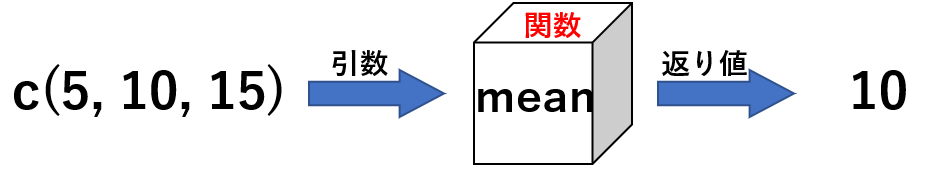
\includegraphics{././image/function_image.png}

}

\caption{図4:関数のイメージ図}

\end{figure}

Rには\textbf{mean関数}という,ベクターの中の数値の平均値を表示してくれる関数があります.上の図では,ベクターである,c(5,
10,
15)を引数として与えると,mean関数は引数を読み取って平均値を計算し,平均値である10を表示してくれます.この,表示される関数の計算結果のことを,\textbf{返り値}と呼びます.

\textbf{関数,引数と返り値}

\begin{Shaded}
\begin{Highlighting}[]
\NormalTok{vec }\OtherTok{\textless{}{-}} \FunctionTok{c}\NormalTok{(}\DecValTok{5}\NormalTok{, }\DecValTok{10}\NormalTok{, }\DecValTok{15}\NormalTok{) }\CommentTok{\# 引数とするベクター}
\FunctionTok{mean}\NormalTok{(vec) }\CommentTok{\# mean関数に引数vecを与えると,10が返り値として返ってくる}
\end{Highlighting}
\end{Shaded}

\begin{verbatim}
[1] 10
\end{verbatim}

Rには,上記の関数以外にも,数値や文字列,データフレームを演算するための関数を数多く備えています.

\textbf{代表的な関数と,関数としての演算子}

\begin{Shaded}
\begin{Highlighting}[]
\FunctionTok{sd}\NormalTok{(vec) }\CommentTok{\# 標準偏差を計算する関数}
\end{Highlighting}
\end{Shaded}

\begin{verbatim}
[1] 5
\end{verbatim}

\begin{Shaded}
\begin{Highlighting}[]
\FunctionTok{median}\NormalTok{(vec) }\CommentTok{\# 中央値を計算する関数}
\end{Highlighting}
\end{Shaded}

\begin{verbatim}
[1] 10
\end{verbatim}

\begin{Shaded}
\begin{Highlighting}[]
\FunctionTok{log10}\NormalTok{(vec) }\CommentTok{\# 常用対数を計算する関数}
\end{Highlighting}
\end{Shaded}

\begin{verbatim}
[1] 0.698970 1.000000 1.176091
\end{verbatim}

\begin{Shaded}
\begin{Highlighting}[]
\FunctionTok{exp}\NormalTok{(vec) }\CommentTok{\# ネイピア数の指数を計算する関数}
\end{Highlighting}
\end{Shaded}

\begin{verbatim}
[1]     148.4132   22026.4658 3269017.3725
\end{verbatim}

\begin{Shaded}
\begin{Highlighting}[]
\FunctionTok{mode}\NormalTok{(}\StringTok{\textasciigrave{}}\AttributeTok{+}\StringTok{\textasciigrave{}}\NormalTok{) }\CommentTok{\# 演算子の+の型はfunction(関数)}
\end{Highlighting}
\end{Shaded}

\begin{verbatim}
[1] "function"
\end{verbatim}

\begin{Shaded}
\begin{Highlighting}[]
\StringTok{\textasciigrave{}}\AttributeTok{+}\StringTok{\textasciigrave{}}\NormalTok{(}\DecValTok{2}\NormalTok{, }\DecValTok{3}\NormalTok{) }\CommentTok{\# 関数なので,引数を2つ取ると足し算になる}
\end{Highlighting}
\end{Shaded}

\begin{verbatim}
[1] 5
\end{verbatim}

\begin{Shaded}
\begin{Highlighting}[]
\FunctionTok{mode}\NormalTok{(}\StringTok{\textasciigrave{}}\AttributeTok{[}\StringTok{\textasciigrave{}}\NormalTok{) }\CommentTok{\# インデックスも関数}
\end{Highlighting}
\end{Shaded}

\begin{verbatim}
[1] "function"
\end{verbatim}

\begin{Shaded}
\begin{Highlighting}[]
\FunctionTok{mode}\NormalTok{(}\StringTok{\textasciigrave{}}\AttributeTok{if}\StringTok{\textasciigrave{}}\NormalTok{) }\CommentTok{\# if(条件分岐)も関数}
\end{Highlighting}
\end{Shaded}

\begin{verbatim}
[1] "function"
\end{verbatim}

\begin{Shaded}
\begin{Highlighting}[]
\FunctionTok{mode}\NormalTok{(}\StringTok{\textasciigrave{}}\AttributeTok{for}\StringTok{\textasciigrave{}}\NormalTok{) }\CommentTok{\# for(繰り返し文)も関数}
\end{Highlighting}
\end{Shaded}

\begin{verbatim}
[1] "function"
\end{verbatim}

\begin{quote}
Rでは,演算子やインデックス指定,条件分岐,繰り返し文も関数です.
\end{quote}

このように,Rでは多くの演算を関数によって処理しています.この性質から,Rは\textbf{関数型言語}であるとされています.

\begin{quote}
正確には,Rは厳密な意味では関数型言語ではないように思います.関数型言語には\href{https://www.haskell.org/}{Haskell}などがありますが,関数型言語では再帰的関数(関数内で関数を呼び出す)ような処理を用いて繰り返し計算を避けるようなものが多いです.Rでも再帰的関数を用いることはできますが,頻繁には使用されません.
\end{quote}

\hypertarget{ux95a2ux6570ux3092ux81eaux4f5cux3059ux308b}{%
\subsection{関数を自作する}\label{ux95a2ux6570ux3092ux81eaux4f5cux3059ux308b}}

どのようなプログラミング言語にも,関数を自作する方法が備わっています.Rでは,\textbf{function文}を用いて関数を自作することができます.関数を変数に代入して用いるのが一般的な関数の作成方法です.function文の書き方は以下の通りです.

\textbf{関数名 \textless- function(引数群)\{引数を使った処理\}}

関数の返り値は,\textbf{return関数}を使って明示することもできますが,単に最後に記載したオブジェクトを返り値とすることもできます.

また,Rではfunctionと書く代わりに,\textbackslash(\,バックスラッシュ)をfunctionの代わりに用いることもできます.

作成した関数を用いて演算するときには,「関数名(引数)」という形で表記します.これはmode関数やclass関数の使い方と同じです.

\textbf{関数を自作する}

\begin{Shaded}
\begin{Highlighting}[]
\CommentTok{\# 引数をそのまま帰す関数}
\NormalTok{return\_selfx }\OtherTok{\textless{}{-}} \ControlFlowTok{function}\NormalTok{(x)\{}\FunctionTok{return}\NormalTok{(x)\} }\CommentTok{\# 返り値をreturn関数で表示}
\NormalTok{return\_selfy }\OtherTok{\textless{}{-}} \ControlFlowTok{function}\NormalTok{(y)\{y\} }\CommentTok{\# 最後に返り値を書く}
\NormalTok{return\_selfz }\OtherTok{\textless{}{-}}\NormalTok{ \textbackslash{}(z)\{z\} }\CommentTok{\# functionの代わりにバックスラッシュを用いる}

\CommentTok{\# どれも同じ演算をする関数になる}
\FunctionTok{return\_selfx}\NormalTok{(}\DecValTok{1}\NormalTok{)}
\end{Highlighting}
\end{Shaded}

\begin{verbatim}
[1] 1
\end{verbatim}

\begin{Shaded}
\begin{Highlighting}[]
\FunctionTok{return\_selfy}\NormalTok{(}\DecValTok{1}\NormalTok{)}
\end{Highlighting}
\end{Shaded}

\begin{verbatim}
[1] 1
\end{verbatim}

\begin{Shaded}
\begin{Highlighting}[]
\FunctionTok{return\_selfz}\NormalTok{(}\DecValTok{1}\NormalTok{)}
\end{Highlighting}
\end{Shaded}

\begin{verbatim}
[1] 1
\end{verbatim}

実際に関数を作るときには,もう少し複雑な処理を\{\}(中かっこ)の中に書きます.処理は一つ一つ改行しながら書き,最後に返り値を書きます.中かっこの中で改行を行っても問題ありませんが,かっこの前側(\{)は,引数のかっこ(「)」)の後に記載されている必要があります.

\textbf{関数内の処理の書き方}

\begin{Shaded}
\begin{Highlighting}[]
\CommentTok{\# sum2関数を作成する}
\NormalTok{sum2 }\OtherTok{\textless{}{-}} \ControlFlowTok{function}\NormalTok{(x, y, z)\{ }\CommentTok{\# 引数はx,y,zの3つ}
\NormalTok{  sum\_of\_xyz }\OtherTok{\textless{}{-}}\NormalTok{ x }\SpecialCharTok{+}\NormalTok{ y }\SpecialCharTok{+}\NormalTok{ z }\CommentTok{\# 引数を足し算する}
\NormalTok{  sum\_of\_xyz }\CommentTok{\# 足し算したものを返り値にする}
\NormalTok{\}}

\FunctionTok{sum2}\NormalTok{(}\AttributeTok{x =} \DecValTok{1}\NormalTok{, }\AttributeTok{y =} \DecValTok{2}\NormalTok{, }\AttributeTok{z =} \DecValTok{3}\NormalTok{)}
\end{Highlighting}
\end{Shaded}

\begin{verbatim}
[1] 6
\end{verbatim}

上の例のように,引数を指定するときには,引数の種類を明示的に記載することもできます.明示的に記載する場合には,\textbf{「引数名=値」}という形で書きます.引数名を省略した場合には,記載した引数の順番に従って,引数が用いられます.

関数を作成するときには,\textbf{引数のデフォルト値}を設定しておくこともできます.デフォルト値が設定されている関数では,その引数を入力しなかったときには,自動的に引数にデフォルト値が入ります.

\textbf{引数のデフォルト値と省略}

\begin{Shaded}
\begin{Highlighting}[]
\NormalTok{sum3 }\OtherTok{\textless{}{-}} \ControlFlowTok{function}\NormalTok{(x, }\AttributeTok{y =} \DecValTok{1}\NormalTok{)\{ }\CommentTok{\# yのデフォルト値を1とする}
  \FunctionTok{return}\NormalTok{(x }\SpecialCharTok{+}\NormalTok{ y)}
\NormalTok{\}}

\FunctionTok{sum3}\NormalTok{(}\AttributeTok{x =} \DecValTok{1}\NormalTok{, }\AttributeTok{y=} \DecValTok{2}\NormalTok{) }\CommentTok{\# 引数を明示的に記載}
\end{Highlighting}
\end{Shaded}

\begin{verbatim}
[1] 3
\end{verbatim}

\begin{Shaded}
\begin{Highlighting}[]
\FunctionTok{sum3}\NormalTok{(}\DecValTok{1}\NormalTok{, }\DecValTok{2}\NormalTok{) }\CommentTok{\# xに1,yに2が入る}
\end{Highlighting}
\end{Shaded}

\begin{verbatim}
[1] 3
\end{verbatim}

\begin{Shaded}
\begin{Highlighting}[]
\FunctionTok{sum3}\NormalTok{(}\DecValTok{1}\NormalTok{) }\CommentTok{\# 引数yが省略されているので,デフォルト値(1)が用いられる}
\end{Highlighting}
\end{Shaded}

\begin{verbatim}
[1] 2
\end{verbatim}

\begin{Shaded}
\begin{Highlighting}[]
\FunctionTok{sum3}\NormalTok{(}\AttributeTok{y=}\DecValTok{1}\NormalTok{) }\CommentTok{\# xはデフォルトが設定されていないので,省略できない}
\end{Highlighting}
\end{Shaded}

\begin{verbatim}
Error in sum3(y = 1): argument "x" is missing, with no default
\end{verbatim}

\hypertarget{ux578bux30afux30e9ux30b9ux306eux78baux8a8dux3068ux5909ux63db}{%
\section{型・クラスの確認と変換}\label{ux578bux30afux30e9ux30b9ux306eux78baux8a8dux3068ux5909ux63db}}

\hypertarget{ux578bux30afux30e9ux30b9ux306eux78baux8a8dis.ux95a2ux6570ux7fa4}{%
\subsection{型・クラスの確認:is.関数群}\label{ux578bux30afux30e9ux30b9ux306eux78baux8a8dis.ux95a2ux6570ux7fa4}}

Rでは,型やクラスを確認するための関数として,typeof関数・mode関数・class関数以外に,\textbf{is.関数}というものを備えています.is.関数を用いると,オブジェクトの型が,ある型と一致しているかどうかを確認することができます.引数が数値であるかどうかは,\textbf{is.numeric関数,is.integer関数,is.double関数}を用いて確認することができます.例えば\textbf{is.numeric(1)はTRUE}を返し,\textbf{is.numeric(``dog'')}はFALSEを返します.このis.関数には,文字列やNA,NaN等を確認する関数もあります.is.関数を以下の表に示します.

\begin{longtable}[]{@{}ll@{}}
\caption{表2:xの型の確認に用いる関数}\tabularnewline
\toprule()
is.関数名 & チェックする型 \\
\midrule()
\endfirsthead
\toprule()
is.関数名 & チェックする型 \\
\midrule()
\endhead
is.numeric(x) & 数値型 \\
is.integer(x) & 整数型 \\
is.double(x) & double型 \\
is.complex & 複素数型 \\
is.character(x) & 文字列型 \\
is.logical(x) & 真偽型 \\
is.factor(x) & 因子型 \\
is.atomic(x) & ベクター \\
is.list(x) & リスト \\
is.matrix(x) & マトリックス \\
is.data.frame(x) & データフレーム \\
is.na(x) & NA \\
is.nan(x) & NaN \\
is.null(x) & NULL \\
is.infinite(x) & 無限大 \\
\bottomrule()
\end{longtable}

is.関数の中では,\textbf{is.na関数}の使用頻度が高いです.is.na関数を用いると,ベクターやデータフレームからNAを含む要素をうまく取り除くことができます.

\textbf{is.関数群}

\begin{Shaded}
\begin{Highlighting}[]
\FunctionTok{c}\NormalTok{(}\FunctionTok{is.numeric}\NormalTok{(}\DecValTok{1}\NormalTok{), }\FunctionTok{is.numeric}\NormalTok{(}\StringTok{"1"}\NormalTok{)) }\CommentTok{\# 文字列("1")は数値ではない}
\end{Highlighting}
\end{Shaded}

\begin{verbatim}
[1]  TRUE FALSE
\end{verbatim}

\begin{Shaded}
\begin{Highlighting}[]
\FunctionTok{c}\NormalTok{(}\FunctionTok{is.integer}\NormalTok{(1L), }\FunctionTok{is.integer}\NormalTok{(}\DecValTok{1}\NormalTok{)) }\CommentTok{\# Lが付いていないとdoubleになる}
\end{Highlighting}
\end{Shaded}

\begin{verbatim}
[1]  TRUE FALSE
\end{verbatim}

\begin{Shaded}
\begin{Highlighting}[]
\FunctionTok{c}\NormalTok{(}\FunctionTok{is.double}\NormalTok{(}\DecValTok{1}\NormalTok{), }\FunctionTok{is.double}\NormalTok{(1L)) }\CommentTok{\# Lが付いているとintegerになる}
\end{Highlighting}
\end{Shaded}

\begin{verbatim}
[1]  TRUE FALSE
\end{verbatim}

\begin{Shaded}
\begin{Highlighting}[]
\FunctionTok{c}\NormalTok{(}\FunctionTok{is.complex}\NormalTok{(}\DecValTok{1}\SpecialCharTok{+}\NormalTok{1i), }\FunctionTok{is.complex}\NormalTok{(}\DecValTok{1}\SpecialCharTok{+}\DecValTok{1}\NormalTok{)) }\CommentTok{\# iがあると複素数になる}
\end{Highlighting}
\end{Shaded}

\begin{verbatim}
[1]  TRUE FALSE
\end{verbatim}

\begin{Shaded}
\begin{Highlighting}[]
\FunctionTok{c}\NormalTok{(}\FunctionTok{is.character}\NormalTok{(}\StringTok{"dog"}\NormalTok{), }\FunctionTok{is.character}\NormalTok{(}\DecValTok{1}\NormalTok{)) }\CommentTok{\# 数値は文字列ではない}
\end{Highlighting}
\end{Shaded}

\begin{verbatim}
[1]  TRUE FALSE
\end{verbatim}

\begin{Shaded}
\begin{Highlighting}[]
\CommentTok{\# 0はFALSE扱いされるが,logicalではない}
\FunctionTok{c}\NormalTok{(}\FunctionTok{is.logical}\NormalTok{(T), }\FunctionTok{is.logical}\NormalTok{(}\DecValTok{0}\NormalTok{), }\FunctionTok{is.logical}\NormalTok{(}\StringTok{"dog"}\NormalTok{)) }
\end{Highlighting}
\end{Shaded}

\begin{verbatim}
[1]  TRUE FALSE FALSE
\end{verbatim}

\begin{Shaded}
\begin{Highlighting}[]
\FunctionTok{c}\NormalTok{(}\FunctionTok{is.factor}\NormalTok{(}\FunctionTok{factor}\NormalTok{(}\DecValTok{1}\NormalTok{)), }\FunctionTok{is.factor}\NormalTok{(}\DecValTok{1}\NormalTok{))}
\end{Highlighting}
\end{Shaded}

\begin{verbatim}
[1]  TRUE FALSE
\end{verbatim}

\begin{Shaded}
\begin{Highlighting}[]
\FunctionTok{c}\NormalTok{(}\FunctionTok{is.atomic}\NormalTok{(}\DecValTok{1}\NormalTok{), }\FunctionTok{is.atomic}\NormalTok{(}\FunctionTok{list}\NormalTok{(}\DecValTok{1}\NormalTok{))) }\CommentTok{\# ベクターはTRUE,リストはFALSE}
\end{Highlighting}
\end{Shaded}

\begin{verbatim}
[1]  TRUE FALSE
\end{verbatim}

\begin{Shaded}
\begin{Highlighting}[]
\FunctionTok{c}\NormalTok{(}\FunctionTok{is.vector}\NormalTok{(}\DecValTok{1}\NormalTok{), }\FunctionTok{is.vector}\NormalTok{(}\FunctionTok{list}\NormalTok{(}\DecValTok{1}\NormalTok{))) }\CommentTok{\# is.vectorもあるが,リストもTRUEになる}
\end{Highlighting}
\end{Shaded}

\begin{verbatim}
[1] TRUE TRUE
\end{verbatim}

\begin{Shaded}
\begin{Highlighting}[]
\FunctionTok{c}\NormalTok{(}\FunctionTok{is.list}\NormalTok{(}\FunctionTok{list}\NormalTok{(}\DecValTok{1}\NormalTok{)), }\FunctionTok{is.list}\NormalTok{(}\DecValTok{1}\NormalTok{))}\CommentTok{\# ベクターはFALSE,リストはTRUE}
\end{Highlighting}
\end{Shaded}

\begin{verbatim}
[1]  TRUE FALSE
\end{verbatim}

\begin{Shaded}
\begin{Highlighting}[]
\FunctionTok{c}\NormalTok{(}\FunctionTok{is.matrix}\NormalTok{(}\FunctionTok{matrix}\NormalTok{(}\DecValTok{1}\NormalTok{, }\AttributeTok{ncol=}\DecValTok{1}\NormalTok{)), }\FunctionTok{is.matrix}\NormalTok{(}\DecValTok{1}\NormalTok{))}
\end{Highlighting}
\end{Shaded}

\begin{verbatim}
[1]  TRUE FALSE
\end{verbatim}

\begin{Shaded}
\begin{Highlighting}[]
\FunctionTok{c}\NormalTok{(}\FunctionTok{is.data.frame}\NormalTok{(}\FunctionTok{data.frame}\NormalTok{(}\DecValTok{1}\NormalTok{)), }\FunctionTok{is.data.frame}\NormalTok{(}\FunctionTok{list}\NormalTok{(}\DecValTok{1}\NormalTok{))) }\CommentTok{\# リストはFALSE}
\end{Highlighting}
\end{Shaded}

\begin{verbatim}
[1]  TRUE FALSE
\end{verbatim}

\begin{Shaded}
\begin{Highlighting}[]
\CommentTok{\# NAとNaNはNA扱い,NULLは無いもの扱い}
\FunctionTok{c}\NormalTok{(}\FunctionTok{is.na}\NormalTok{(}\ConstantTok{NA}\NormalTok{), }\FunctionTok{is.na}\NormalTok{(}\DecValTok{1}\NormalTok{), }\FunctionTok{is.na}\NormalTok{(}\ConstantTok{NaN}\NormalTok{), }\FunctionTok{is.na}\NormalTok{(}\ConstantTok{Inf}\NormalTok{), }\FunctionTok{is.na}\NormalTok{(}\ConstantTok{NULL}\NormalTok{)) }
\end{Highlighting}
\end{Shaded}

\begin{verbatim}
[1]  TRUE FALSE  TRUE FALSE
\end{verbatim}

\begin{Shaded}
\begin{Highlighting}[]
\CommentTok{\# NULLは無いもの扱い}
\FunctionTok{c}\NormalTok{(}\FunctionTok{is.nan}\NormalTok{(}\ConstantTok{NA}\NormalTok{), }\FunctionTok{is.nan}\NormalTok{(}\DecValTok{1}\NormalTok{), }\FunctionTok{is.nan}\NormalTok{(}\ConstantTok{NaN}\NormalTok{), }\FunctionTok{is.nan}\NormalTok{(}\ConstantTok{Inf}\NormalTok{), }\FunctionTok{is.nan}\NormalTok{(}\ConstantTok{NULL}\NormalTok{))}
\end{Highlighting}
\end{Shaded}

\begin{verbatim}
[1] FALSE FALSE  TRUE FALSE
\end{verbatim}

\begin{Shaded}
\begin{Highlighting}[]
\CommentTok{\# NULLを評価する}
\FunctionTok{c}\NormalTok{(}\FunctionTok{is.null}\NormalTok{(}\ConstantTok{NA}\NormalTok{), }\FunctionTok{is.null}\NormalTok{(}\DecValTok{1}\NormalTok{), }\FunctionTok{is.null}\NormalTok{(}\ConstantTok{NaN}\NormalTok{), }\FunctionTok{is.null}\NormalTok{(}\ConstantTok{Inf}\NormalTok{), }\FunctionTok{is.null}\NormalTok{(}\ConstantTok{NULL}\NormalTok{)) }
\end{Highlighting}
\end{Shaded}

\begin{verbatim}
[1] FALSE FALSE FALSE FALSE  TRUE
\end{verbatim}

\begin{Shaded}
\begin{Highlighting}[]
\CommentTok{\# NULLは無いもの扱い}
\FunctionTok{c}\NormalTok{(}\FunctionTok{is.infinite}\NormalTok{(}\ConstantTok{NA}\NormalTok{), }\FunctionTok{is.infinite}\NormalTok{(}\DecValTok{1}\NormalTok{), }\FunctionTok{is.infinite}\NormalTok{(}\ConstantTok{NaN}\NormalTok{), }\FunctionTok{is.infinite}\NormalTok{(}\ConstantTok{Inf}\NormalTok{), }\FunctionTok{is.infinite}\NormalTok{(}\ConstantTok{NULL}\NormalTok{)) }
\end{Highlighting}
\end{Shaded}

\begin{verbatim}
[1] FALSE FALSE FALSE  TRUE
\end{verbatim}

\begin{quote}
ベクターはis.atomic関数で評価します.これは,ベクターのことをatomic
vectorと呼ぶためです.atomic
vectorはvectorと同じ意味を持ちます.エラーには時々このatomic
vectorという表記が出てきますが,これは通常のベクターのことを述べているだけで,atomic
vectorという特別なものがあるわけではありません.
\end{quote}

\hypertarget{ux578bux30afux30e9ux30b9ux306eux5909ux63dbas.ux95a2ux6570ux7fa4}{%
\subsection{型・クラスの変換:as.関数群}\label{ux578bux30afux30e9ux30b9ux306eux5909ux63dbas.ux95a2ux6570ux7fa4}}

is.関数はデータのクラスや型をチェックし,真偽値を返す関数です.Rには,関数名がよく似た\textbf{as.関数}があります.\textbf{as.関数}は,引数の型を指定した型に変換する関数です.例えば,\textbf{as.numeric関数}は引数をnumericに変換する関数です.as.関数を以下の表に示します.

\begin{longtable}[]{@{}ll@{}}
\caption{表3:xの型の変換に用いる関数}\tabularnewline
\toprule()
as.関数名 & 変換する型 \\
\midrule()
\endfirsthead
\toprule()
as.関数名 & 変換する型 \\
\midrule()
\endhead
as.numeric(x) & 数値型に変換 \\
as.integer(x) & 整数型に変換 \\
as.double(x) & double型に変換 \\
as.complex & 複素数型に変換 \\
as.character(x) & 文字列型に変換 \\
as.logical(x) & 真偽型に変換 \\
as.factor(x) & 因子型に変換 \\
as.Date & 日時型に変換 \\
as.POSIXct & POSIXct型に変換 \\
as.POSIXlt & POSIXlt型に変換 \\
as.list(x) & リストに変換 \\
as.matrix(x) & マトリックスに変換 \\
as.data.frame(x) & データフレームに変換 \\
as.null(x) & NULLに変換 \\
\bottomrule()
\end{longtable}

\textbf{as.関数群}

\begin{Shaded}
\begin{Highlighting}[]
\FunctionTok{as.numeric}\NormalTok{(}\ConstantTok{TRUE}\NormalTok{)}
\end{Highlighting}
\end{Shaded}

\begin{verbatim}
[1] 1
\end{verbatim}

\begin{Shaded}
\begin{Highlighting}[]
\FunctionTok{as.integer}\NormalTok{(}\FloatTok{1.1}\NormalTok{)}
\end{Highlighting}
\end{Shaded}

\begin{verbatim}
[1] 1
\end{verbatim}

\begin{Shaded}
\begin{Highlighting}[]
\FunctionTok{as.double}\NormalTok{(1L)}
\end{Highlighting}
\end{Shaded}

\begin{verbatim}
[1] 1
\end{verbatim}

\begin{Shaded}
\begin{Highlighting}[]
\FunctionTok{as.complex}\NormalTok{(}\DecValTok{1}\NormalTok{)}
\end{Highlighting}
\end{Shaded}

\begin{verbatim}
[1] 1+0i
\end{verbatim}

\begin{Shaded}
\begin{Highlighting}[]
\FunctionTok{as.character}\NormalTok{(}\DecValTok{1}\NormalTok{)}
\end{Highlighting}
\end{Shaded}

\begin{verbatim}
[1] "1"
\end{verbatim}

\begin{Shaded}
\begin{Highlighting}[]
\FunctionTok{c}\NormalTok{(}\FunctionTok{as.logical}\NormalTok{(}\DecValTok{1}\NormalTok{), }\FunctionTok{as.logical}\NormalTok{(}\DecValTok{0}\NormalTok{))}
\end{Highlighting}
\end{Shaded}

\begin{verbatim}
[1]  TRUE FALSE
\end{verbatim}

\begin{Shaded}
\begin{Highlighting}[]
\FunctionTok{as.factor}\NormalTok{(}\FunctionTok{c}\NormalTok{(}\StringTok{"dog"}\NormalTok{, }\StringTok{"cat"}\NormalTok{))}
\end{Highlighting}
\end{Shaded}

\begin{verbatim}
[1] dog cat
Levels: cat dog
\end{verbatim}

\begin{Shaded}
\begin{Highlighting}[]
\FunctionTok{as.Date}\NormalTok{(}\StringTok{"2022{-}02{-}22"}\NormalTok{) }\CommentTok{\# わかりにくいが,日付型になっている}
\end{Highlighting}
\end{Shaded}

\begin{verbatim}
[1] "2022-02-22"
\end{verbatim}

\begin{Shaded}
\begin{Highlighting}[]
\CommentTok{\# わかりにくいが,日時型になっている}
\FunctionTok{as.POSIXct}\NormalTok{(}\StringTok{"2022{-}02{-}22 15:00:00"}\NormalTok{)}
\end{Highlighting}
\end{Shaded}

\begin{verbatim}
[1] "2022-02-22 15:00:00 JST"
\end{verbatim}

\begin{Shaded}
\begin{Highlighting}[]
\FunctionTok{as.POSIXlt}\NormalTok{(}\StringTok{"2022{-}02{-}22 15:00:00"}\NormalTok{)}
\end{Highlighting}
\end{Shaded}

\begin{verbatim}
[1] "2022-02-22 15:00:00 JST"
\end{verbatim}

\begin{Shaded}
\begin{Highlighting}[]
\FunctionTok{as.list}\NormalTok{(}\DecValTok{1}\NormalTok{)}
\end{Highlighting}
\end{Shaded}

\begin{verbatim}
[[1]]
[1] 1
\end{verbatim}

\begin{Shaded}
\begin{Highlighting}[]
\FunctionTok{as.data.frame}\NormalTok{(}\FunctionTok{list}\NormalTok{(}\DecValTok{1}\NormalTok{, }\DecValTok{1}\NormalTok{))}
\end{Highlighting}
\end{Shaded}

\begin{verbatim}
  X1 X1.1
1  1    1
\end{verbatim}

\begin{Shaded}
\begin{Highlighting}[]
\FunctionTok{as.matrix}\NormalTok{(}\FunctionTok{data.frame}\NormalTok{(}\AttributeTok{x=}\DecValTok{1}\NormalTok{, }\AttributeTok{y=}\DecValTok{1}\NormalTok{))}
\end{Highlighting}
\end{Shaded}

\begin{verbatim}
     x y
[1,] 1 1
\end{verbatim}

\begin{Shaded}
\begin{Highlighting}[]
\FunctionTok{as.null}\NormalTok{(}\DecValTok{1}\NormalTok{)}
\end{Highlighting}
\end{Shaded}

\begin{verbatim}
NULL
\end{verbatim}

\begin{quote}
as.関数群は変換できない場合にNAを返すときがありますので,注意が必要です.as.関数はそれほど使用頻度は高くありませんが,行列をデータフレームに変換するときなどに使用することがあります.
\end{quote}

\hypertarget{ux4e88ux7d04ux8a9e}{%
\section{予約語}\label{ux4e88ux7d04ux8a9e}}

上の例では関数や変数には名前をつけていますが,関数名や変数名の付け方にはルールがあります.

\begin{itemize}
\tightlist
\item
  名前の始めに数値(1,2など)をつけることはできない
\item
  名前の始めにアンダーバー(\_)を用いることはできない
\item
  大文字と小文字は区別される(SUMとsumは別扱い)
\item
  演算子や記号(!や?,+,-,\# など)は使えない
\item
  \textbf{予約語}を用いることはできない
\end{itemize}

\textbf{予約語(reserved
word)}とは,R言語がすでに役割を与えているために,関数名や変数名には使用できない文字列です.Rで設定されている予約語は以下の通りです.

\begin{itemize}
\tightlist
\item
  if
\item
  else
\item
  repeat
\item
  while
\item
  function\\
\item
  for
\item
  in
\item
  next
\item
  break
\item
  TRUE
\item
  FALSE
\item
  NULL
\item
  Inf
\item
  NaN
\item
  NA
\item
  NA\_integer\_
\item
  NA\_real\_
\item
  NA\_complex\_
\item
  NA\_character\_
\item
  \ldots{}
\item
  ..1
\item
  ..2
\end{itemize}

\begin{quote}
Rでは,ピリオド(.)が予約語に含まれていないため,変数名にピリオドを利用することができます.ただし,他の言語ではこのピリオドをメソッド(method)という,関数の仲間のようなものに用いることが多く,勘違いを起こしやすい表記になります.Rでも変数名にピリオドを用いないほうがよいとされています.
\end{quote}

\bookmarksetup{startatroot}

\hypertarget{ux6761ux4ef6ux5224ux65adcontrol-structures}{%
\chapter{条件判断(Control
structures)}\label{ux6761ux4ef6ux5224ux65adcontrol-structures}}

\hypertarget{ux6761ux4ef6ux5224ux65adux3068ux306f}{%
\section{条件判断とは?}\label{ux6761ux4ef6ux5224ux65adux3068ux306f}}

プログラミングでは,ある条件のときはこの処理,別の条件のときはこの処理\ldots,といった具合に,条件によって行う処理を変えたいことがよくあります.例えばじゃんけんが典型的な例です.じゃんけんでは,出した手の条件によって,勝ちと負けという2つの処理を行うことになります.このように,条件によって処理を変えることを,\textbf{条件判断}と呼びます.

\hypertarget{ux6761ux4ef6ux3068ux771fux507dux5024logical}{%
\section{条件と真偽値(logical)}\label{ux6761ux4ef6ux3068ux771fux507dux5024logical}}

条件として用いられるのは,\textbf{真偽値(logical)}です.真偽値はTRUE(真)とFALSE(偽)の2つの値を持ちます.真偽値はそれそのものを用いる場合と,比較演算子の演算結果として得る場合があります.Rでは,\textbf{TRUEをT,FALSEをF}と表記しても,真偽値を表すことになります.

\textbf{}

\begin{Shaded}
\begin{Highlighting}[]
\ConstantTok{TRUE}
\DocumentationTok{\#\# [1] TRUE}
\ConstantTok{FALSE}
\DocumentationTok{\#\# [1] FALSE}
\NormalTok{T}
\DocumentationTok{\#\# [1] TRUE}
\NormalTok{F}
\DocumentationTok{\#\# [1] FALSE}
\FunctionTok{c}\NormalTok{(T, F, T, F) }\CommentTok{\# logicalはベクターにもできる}
\DocumentationTok{\#\# [1]  TRUE FALSE  TRUE FALSE}
\DecValTok{1} \SpecialCharTok{\textless{}} \DecValTok{3} \CommentTok{\# 3は1より大きいのでTRUE}
\DocumentationTok{\#\# [1] TRUE}
\DecValTok{1} \SpecialCharTok{\textgreater{}} \DecValTok{3} \CommentTok{\# 1は3より大きくないのでFALSE}
\DocumentationTok{\#\# [1] FALSE}
\end{Highlighting}
\end{Shaded}

\hypertarget{ux6570ux5024ux3068ux3057ux3066ux306eux771fux507dux5024}{%
\section{数値としての真偽値}\label{ux6570ux5024ux3068ux3057ux3066ux306eux771fux507dux5024}}

真偽値は,Rの内部的には数字として取り扱われています.Rでは\textbf{TRUEは1,FALSEは0}と同一です.ですので,ベクター中のTRUEの数を足し算で計算することができます.逆に,\textbf{0がFALSE,0以外がTRUE}と同一として扱われる場合もあります.条件判断では0をFALSEの代わりに用いる場合もあります.

\begin{quote}
RではTRUEが1,FALSEが0ですが,他の言語ではFALSEが-1のものもあります.言語によりTRUE/FALSEの仕様は異なります.
\end{quote}

\textbf{数値としての真偽値}

\begin{Shaded}
\begin{Highlighting}[]
\NormalTok{T }\SpecialCharTok{+}\NormalTok{ T }\SpecialCharTok{+}\NormalTok{ F }\CommentTok{\# 足し算すると2が返ってくる}
\DocumentationTok{\#\# [1] 2}
\NormalTok{vec }\OtherTok{\textless{}{-}} \FunctionTok{c}\NormalTok{(T, T, F, T, F, T, F)}
\FunctionTok{sum}\NormalTok{(vec) }\CommentTok{\# sumはベクターの要素を足し算する関数}
\DocumentationTok{\#\# [1] 4}
\end{Highlighting}
\end{Shaded}

\hypertarget{ux8ad6ux7406ux6f14ux7b97ux5b50}{%
\section{論理演算子}\label{ux8ad6ux7406ux6f14ux7b97ux5b50}}

真偽値は,\textbf{論理演算子}による計算に使うことができます.Rでの論理演算子は\textbf{\&,\&\&,\textbar,\textbar\textbar{}}の4つです.このうち,\&\&と\textbar\textbar は,ベクターの\textbf{始めの値だけ}を評価するという特徴を持っています(最近のRのバージョンでは警告が出ます).\&\&と\textbar\textbar を用いるとプログラムが予想外の挙動を取ることがあるので,できるだけ\&と\textbar だけを用いたほうがよいでしょう.RにはNAND,XOR,NORなどを表す専用の論理演算子はありません.

\begin{longtable}[]{@{}ll@{}}
\caption{表1:Rで使える論理演算子}\tabularnewline
\toprule()
論理演算子 & 演算子の意味 \\
\midrule()
\endfirsthead
\toprule()
論理演算子 & 演算子の意味 \\
\midrule()
\endhead
\& & 論理積(AかつB) \\
\&\& & 論理積(ベクターの始めの要素のみ評価) \\
\textbar{} & 論理和(AまたはB) \\
\textbar\textbar{} & 論理和(ベクターの始めの要素のみ評価) \\
! & 否定演算子(真偽を反転) \\
\bottomrule()
\end{longtable}

\textbf{}

\begin{Shaded}
\begin{Highlighting}[]
\NormalTok{logic1 }\OtherTok{\textless{}{-}} \FunctionTok{c}\NormalTok{(T, F)}
\NormalTok{logic2 }\OtherTok{\textless{}{-}} \FunctionTok{c}\NormalTok{(F, F)}
\NormalTok{logic1 }\SpecialCharTok{\&}\NormalTok{ logic2 }\CommentTok{\# \& は論理積(AND)}
\DocumentationTok{\#\# [1] FALSE FALSE}

\NormalTok{logic1 }\SpecialCharTok{|}\NormalTok{ logic2 }\CommentTok{\# | は論理和(OR)}
\DocumentationTok{\#\# [1]  TRUE FALSE}

\NormalTok{logic1 }\SpecialCharTok{\&\&}\NormalTok{ logic2 }\CommentTok{\# 1番目の項目同士のみを比較する}
\DocumentationTok{\#\# Error in logic1 \&\& logic2: \textquotesingle{}length = 2\textquotesingle{} in coercion to \textquotesingle{}logical(1)\textquotesingle{}}

\NormalTok{logic1 }\SpecialCharTok{||}\NormalTok{ logic2}
\DocumentationTok{\#\# Error in logic1 || logic2: \textquotesingle{}length = 2\textquotesingle{} in coercion to \textquotesingle{}logical(1)\textquotesingle{}}
\end{Highlighting}
\end{Shaded}

論理演算子として,\textbf{!(エクスクラメーションマーク,否定演算子)}も用いることができます.!は真偽値の前に置くことで,真偽値を反転(TRUEをFALSEに,FALSEをTRUEに)させます.

\textbf{!による論理値の反転}

\begin{Shaded}
\begin{Highlighting}[]
\SpecialCharTok{!}\ConstantTok{TRUE}
\DocumentationTok{\#\# [1] FALSE}
\SpecialCharTok{!}\ConstantTok{FALSE}
\DocumentationTok{\#\# [1] TRUE}

\SpecialCharTok{!}\NormalTok{(}\DecValTok{1} \SpecialCharTok{\textless{}} \DecValTok{3}\NormalTok{)}
\DocumentationTok{\#\# [1] FALSE}
\SpecialCharTok{!}\NormalTok{(}\DecValTok{1} \SpecialCharTok{\textgreater{}} \DecValTok{3}\NormalTok{)}
\DocumentationTok{\#\# [1] TRUE}
\end{Highlighting}
\end{Shaded}

\hypertarget{ux6761ux4ef6ux5206ux5c90ux306eux6587}{%
\section{条件分岐の文}\label{ux6761ux4ef6ux5206ux5c90ux306eux6587}}

上記のように,比較演算子や論理演算子を用いると,真偽値を得ることができます.この真偽値に従い,行う処理を変えるものを,\textbf{条件分岐}と呼びます.条件分岐では,条件分岐の文(Control
structures)というものが用いられます.Rでは,条件分岐の文として,\textbf{if文とswitch文}の2つが設定されています.

\begin{longtable}[]{@{}ll@{}}
\caption{表2:Rで使える条件分岐}\tabularnewline
\toprule()
条件分岐 & 条件分岐の形式 \\
\midrule()
\endfirsthead
\toprule()
条件分岐 & 条件分岐の形式 \\
\midrule()
\endhead
if文 & if(条件式)\{TRUEのときの演算\}else\{FALSEのときの演算\} \\
ifelse関数 & ifelse(条件式, TRUEのときの演算, FALSEのときの演算) \\
switch文 & switch(評価する値, 評価の既定値=既定値のときの演算) \\
\bottomrule()
\end{longtable}

\hypertarget{ifux6587}{%
\subsection{if文}\label{ifux6587}}

if文は最もシンプルな条件分岐の文です.if文では,\textbf{条件式}に従い,実行する処理が変わります.Rでのif文は,以下の形を取ります.

\textbf{if(条件式)\{TRUEのときに実施する処理\}}

条件式を\textbf{if()}のカッコの中に書きます.if文は1行で書くこともできますし,複数行に渡って書くこともできます.複数行に処理を書くときには,\textbf{中括弧(\{\})}を条件式の後に書き,中括弧の中に処理を書きます.

\textbf{if文の使い方}

\begin{Shaded}
\begin{Highlighting}[]
\ControlFlowTok{if}\NormalTok{(}\ConstantTok{TRUE}\NormalTok{) }\StringTok{"Hello R"} \CommentTok{\# 1行で書く場合("Hello R"が返ってくる)}
\DocumentationTok{\#\# [1] "Hello R"}
\ControlFlowTok{if}\NormalTok{(}\ConstantTok{FALSE}\NormalTok{) }\StringTok{"Hello FALSE"} \CommentTok{\# 条件式がFALSEなので,何も返ってこない}

\ControlFlowTok{if}\NormalTok{(}\ConstantTok{TRUE}\NormalTok{)\{ }\CommentTok{\# 複数行で書く時には中括弧(\{\})を用いる}
  \StringTok{"Hello R"}
\NormalTok{\}}
\DocumentationTok{\#\# [1] "Hello R"}

\ControlFlowTok{if}\NormalTok{(}\ConstantTok{FALSE}\NormalTok{)\{}\StringTok{"Hello FALSE"}\NormalTok{\} }\CommentTok{\# 1行のif文で中括弧を使ってもよい}
\end{Highlighting}
\end{Shaded}

if文の条件が0のときには,0がFALSEと判断されて,処理が実行されません.一方で条件が0以外である場合には,TRUEであると判断されて処理が実行されます.if(0)とするとその処理が行われないので,\textbf{Rではif(0)がコメントや処理したくない部分を指定するときに使われる}こともあります.

\textbf{条件式が数値の時のif文}

\begin{Shaded}
\begin{Highlighting}[]
\ControlFlowTok{if}\NormalTok{(}\DecValTok{0}\NormalTok{)\{}\StringTok{"0はFALSEなので,これは表示されません"}\NormalTok{\}}

\ControlFlowTok{if}\NormalTok{(}\SpecialCharTok{{-}}\DecValTok{1}\NormalTok{)\{}\StringTok{"{-}1はTRUE扱いなので,表示されます"}\NormalTok{\}}
\DocumentationTok{\#\# [1] "{-}1はTRUE扱いなので,表示されます"}

\ControlFlowTok{if}\NormalTok{(}\SpecialCharTok{{-}}\FloatTok{0.005}\NormalTok{)\{}\StringTok{"0以外はTRUEとして処理されます"}\NormalTok{\}}
\DocumentationTok{\#\# [1] "0以外はTRUEとして処理されます"}
\end{Highlighting}
\end{Shaded}

\hypertarget{if-elseux6587}{%
\subsubsection{if else文}\label{if-elseux6587}}

if文はさらに条件を分岐させることもできます.条件を追加する場合には,if文の後に,\textbf{else()}を繋げます.\textbf{else()}のカッコの中に2つ目の条件を書くことで,条件を分離させることができます.\textbf{else}だけを書いて,elseの条件式をつけない場合には,どの条件にも合わない時に実行する処理になります.ですので,if
else文は以下の形を取ります.

\textbf{if(条件式1)\{} \textbf{式1がTRUEのときの処理}\\
\textbf{\}else if(条件式2)\{}\\
\textbf{式1がFALSE,式2がTRUEのときの処理}\\
\textbf{\}else\{}\\
\textbf{式1,2がFALSEのときの処理\}}

\textbf{if else文}

\begin{Shaded}
\begin{Highlighting}[]
\NormalTok{x }\OtherTok{\textless{}{-}} \DecValTok{2} \CommentTok{\# xは2}

\CommentTok{\# xは2なので,2番目の処理が返ってくる}
\ControlFlowTok{if}\NormalTok{(x }\SpecialCharTok{==} \DecValTok{1}\NormalTok{)\{   }\CommentTok{\# =が1つだと代入になるのでエラーが出る}
  \StringTok{"first"}
\NormalTok{\} }\ControlFlowTok{else} \ControlFlowTok{if}\NormalTok{(x }\SpecialCharTok{==} \DecValTok{2}\NormalTok{)\{}
  \StringTok{"second"}
\NormalTok{\} }\ControlFlowTok{else}\NormalTok{ \{}
  \StringTok{"others"}
\NormalTok{\}}
\DocumentationTok{\#\# [1] "second"}
\end{Highlighting}
\end{Shaded}

\hypertarget{ifelseux95a2ux6570}{%
\subsubsection{ifelse関数}\label{ifelseux95a2ux6570}}

条件分岐が2つしかない場合には,\textbf{ifelse関数}を用いることもできます.ifelse関数は3つの引数,「(条件式),(TRUEのときの処理),(FALSEのときの処理)」を取ります.条件が1つだけで,簡単な処理のみを行うのであればifelse関数で十分な場合もあります.

\textbf{ifelse関数}

\begin{Shaded}
\begin{Highlighting}[]
\CommentTok{\# TRUEなので2番目の処理が返ってくる}
\FunctionTok{ifelse}\NormalTok{(}\DecValTok{1} \SpecialCharTok{\textless{}} \DecValTok{3}\NormalTok{, }\StringTok{"one smaller than three"}\NormalTok{, }\StringTok{"one does not smaller than three"}\NormalTok{)}
\DocumentationTok{\#\# [1] "one smaller than three"}

\CommentTok{\# FALSEなので3番目の処理が返ってくる}
\FunctionTok{ifelse}\NormalTok{(}\DecValTok{1} \SpecialCharTok{\textgreater{}} \DecValTok{3}\NormalTok{, }\StringTok{"one larger than three"}\NormalTok{, }\StringTok{"one does not larger than three"}\NormalTok{) }
\DocumentationTok{\#\# [1] "one does not larger than three"}
\end{Highlighting}
\end{Shaded}

\hypertarget{switchux6587}{%
\subsection{switch文}\label{switchux6587}}

条件式ではなく,特定の値に対応して処理を変えたい場合には,\textbf{switch文}を用います.switch文では,\textbf{始めの引数が条件を指定する値,それに続く引数が条件に対応した処理}となります.条件を指定する値には,数値または文字列を用いることができます.条件が数値の場合と文字列の場合では,やや使い方が異なります.

\textbf{switch文(条件が数値のとき)}

\begin{Shaded}
\begin{Highlighting}[]
\CommentTok{\# 条件が1のときは,2番目の引数の処理が返ってくる}
\ControlFlowTok{switch}\NormalTok{(}\DecValTok{1}\NormalTok{, }\StringTok{"first"}\NormalTok{, }\StringTok{"second"}\NormalTok{, }\StringTok{"third"}\NormalTok{) }
\DocumentationTok{\#\# [1] "first"}

\CommentTok{\# 条件が2のときは,3番目の引数の処理が返ってくる}
\ControlFlowTok{switch}\NormalTok{(}\DecValTok{2}\NormalTok{, }\StringTok{"first"}\NormalTok{, }\StringTok{"second"}\NormalTok{, }\StringTok{"third"}\NormalTok{) }
\DocumentationTok{\#\# [1] "second"}

\CommentTok{\# 条件が5のときは,6番目の引数の処理がないので何も返ってこない}
\ControlFlowTok{switch}\NormalTok{(}\DecValTok{5}\NormalTok{, }\StringTok{"first"}\NormalTok{, }\StringTok{"second"}\NormalTok{, }\StringTok{"third"}\NormalTok{) }
\end{Highlighting}
\end{Shaded}

\textbf{switch文(条件が文字列のとき)}

\begin{Shaded}
\begin{Highlighting}[]
\CommentTok{\# 条件式に対応したもの(=で繋いだもの)が返ってくる}
\ControlFlowTok{switch}\NormalTok{(}\StringTok{"dog"}\NormalTok{, }\AttributeTok{dog =} \StringTok{"犬"}\NormalTok{, }\AttributeTok{cat =} \StringTok{"猫"}\NormalTok{, }\AttributeTok{monkey =} \StringTok{"猿"}\NormalTok{, }\AttributeTok{pig =} \StringTok{"豚"}\NormalTok{)}
\DocumentationTok{\#\# [1] "犬"}

\ControlFlowTok{switch}\NormalTok{(}\StringTok{"monkey"}\NormalTok{, }\AttributeTok{dog =} \StringTok{"犬"}\NormalTok{, }\AttributeTok{cat =} \StringTok{"猫"}\NormalTok{, }\AttributeTok{monkey =} \StringTok{"猿"}\NormalTok{, }\AttributeTok{pig =} \StringTok{"豚"}\NormalTok{)}
\DocumentationTok{\#\# [1] "猿"}

\CommentTok{\# horseは引数に登録していないので,何も返ってこない}
\ControlFlowTok{switch}\NormalTok{(}\StringTok{"horse"}\NormalTok{, }\AttributeTok{dog =} \StringTok{"犬"}\NormalTok{, }\AttributeTok{cat =} \StringTok{"猫"}\NormalTok{, }\AttributeTok{monkey =} \StringTok{"猿"}\NormalTok{, }\AttributeTok{pig =} \StringTok{"豚"}\NormalTok{)}
\end{Highlighting}
\end{Shaded}

\begin{quote}
インストールしたばかりのRでは,上記のif文,if
else文,ifelse関数,switch文しか使えませんが,\textbf{ライブラリ}というものを用いると,他の条件分岐(if\_else関数やcase\_when文)などを用いることもできます.詳細については他の章で説明します.
\end{quote}

\bookmarksetup{startatroot}

\hypertarget{ux7e70ux308aux8fd4ux3057ux6587looping}{%
\chapter{繰り返し文(Looping)}\label{ux7e70ux308aux8fd4ux3057ux6587looping}}

コンピューターのいいところは,\textbf{同じことを繰り返しても疲れないこと}です.Excelで表を作るときに,コピーアンドペーストを何百回も繰り返し,何時間も費やしたことがある方は多いかと思います.このような繰り返しがあっても,すべてをコンピューターに任せることができれば,コンピューターは疲れることなく,一瞬で繰り返し作業を終えてくれます.

ただし,コンピューターに繰り返し作業をしてもらいたければ,具体的に繰り返し作業を指示しないといけません.プログラミングでコンピューターに繰り返し作業を指示するためのものが,\textbf{繰り返し文}です.Rでは繰り返し文として,\textbf{for文,while文,repeat文}の3つが登録されています.

\begin{longtable}[]{@{}ll@{}}
\caption{表1:Rで使える繰り返し文}\tabularnewline
\toprule()
繰り返し文 & 繰り返し文の形式 \\
\midrule()
\endfirsthead
\toprule()
繰り返し文 & 繰り返し文の形式 \\
\midrule()
\endhead
for文 & for(i in ベクター)\{繰り返す処理\} \\
while文 & while(条件式)\{TRUEの時に繰り返す処理\} \\
repeat文 & repeat\{breakまで繰り返す処理\} \\
\bottomrule()
\end{longtable}

\hypertarget{forux6587}{%
\section{for文}\label{forux6587}}

\textbf{for文}はRで,そして他の言語でもよく設定されている,最も典型的な繰り返し文の一つです.Rでは,for文は,

\textbf{for(繰り返しの条件)\{繰り返す処理\}}

という形で表記します.このうち,繰り返しの条件に関しては,

\textbf{for(i in c(1, 2, 3, 4, 5))}

といった形で,\textbf{「変数 in
ベクター」}という形で書きます.これは,ベクターの要素を前から順番に変数に入れていく,ということを意味しています.少し実際に試してみましょう.

\begin{quote}
下のfor文で用いている\textbf{print関数}は,オブジェクトを表示させるための関数です.for文の処理では,オブジェクトの表示にはprint関数を用いる必要があります.また,for文で用いる変数名にはiを用いるのが普通です.このiはイテレーター(iterator,繰り返すもの)の略だと思いますが,よくわかりません.i以降の変数として,j,k\ldots とアルファベット順に使っていくことが多いです.
\end{quote}

\textbf{for文での繰り返し処理}

\begin{Shaded}
\begin{Highlighting}[]
\ControlFlowTok{for}\NormalTok{(i }\ControlFlowTok{in} \FunctionTok{c}\NormalTok{(}\DecValTok{1}\NormalTok{, }\DecValTok{2}\NormalTok{, }\DecValTok{3}\NormalTok{, }\DecValTok{4}\NormalTok{, }\DecValTok{5}\NormalTok{))\{}\FunctionTok{print}\NormalTok{(i)\} }\CommentTok{\# ベクターの要素をiに入れて,iを表示する}
\DocumentationTok{\#\# [1] 1}
\DocumentationTok{\#\# [1] 2}
\DocumentationTok{\#\# [1] 3}
\DocumentationTok{\#\# [1] 4}
\DocumentationTok{\#\# [1] 5}

\ControlFlowTok{for}\NormalTok{(i }\ControlFlowTok{in} \FunctionTok{c}\NormalTok{(}\StringTok{"dog"}\NormalTok{, }\StringTok{"cat"}\NormalTok{, }\StringTok{"pig"}\NormalTok{, }\StringTok{"horse"}\NormalTok{))\{}\FunctionTok{print}\NormalTok{(i)\} }\CommentTok{\# 文字列のベクターでも同じ}
\DocumentationTok{\#\# [1] "dog"}
\DocumentationTok{\#\# [1] "cat"}
\DocumentationTok{\#\# [1] "pig"}
\DocumentationTok{\#\# [1] "horse"}
\end{Highlighting}
\end{Shaded}

iにベクターの要素が前から順番に代入されているのがわかると思います.for文では,このinの後のベクターとして連続した整数を用いる場合が多いのですが,整数の数が多かったり,繰り返したい回数がとても多いと,いちいちc関数でベクターを作るのは大変です.Rでは,このような連続した数値のベクターを作るために,\textbf{「:(コロン)」}を用いることができます.コロンを用いたベクターの作り方は以下の通りです.

\textbf{:(コロン)を用いたベクターの作成}

\begin{Shaded}
\begin{Highlighting}[]
\DecValTok{1}\SpecialCharTok{:}\DecValTok{5}
\DocumentationTok{\#\# [1] 1 2 3 4 5}
\DecValTok{10}\SpecialCharTok{:}\DecValTok{20}
\DocumentationTok{\#\#  [1] 10 11 12 13 14 15 16 17 18 19 20}
\FloatTok{0.5}\SpecialCharTok{:}\FloatTok{5.5}
\DocumentationTok{\#\# [1] 0.5 1.5 2.5 3.5 4.5 5.5}
\end{Highlighting}
\end{Shaded}

for文をコロンを使用して,以下のような形で書くことができます.

\textbf{コロンを使ったfor文}

\begin{Shaded}
\begin{Highlighting}[]
\ControlFlowTok{for}\NormalTok{(i }\ControlFlowTok{in} \DecValTok{1}\SpecialCharTok{:}\DecValTok{5}\NormalTok{)\{}
  \FunctionTok{print}\NormalTok{(i }\SpecialCharTok{{-}} \DecValTok{1}\NormalTok{)}
\NormalTok{\}}
\DocumentationTok{\#\# [1] 0}
\DocumentationTok{\#\# [1] 1}
\DocumentationTok{\#\# [1] 2}
\DocumentationTok{\#\# [1] 3}
\DocumentationTok{\#\# [1] 4}
\end{Highlighting}
\end{Shaded}

ベクターを変数としてあらかじめ準備しておけば,ベクターの要素に対して同じ処理を繰り返す事もできます.

\textbf{変数を使ったfor文}

\begin{Shaded}
\begin{Highlighting}[]
\NormalTok{vec }\OtherTok{\textless{}{-}} \FunctionTok{c}\NormalTok{(}\StringTok{"dog"}\NormalTok{, }\StringTok{"cat"}\NormalTok{, }\StringTok{"pig"}\NormalTok{, }\StringTok{"horse"}\NormalTok{)}
\ControlFlowTok{for}\NormalTok{(i }\ControlFlowTok{in}\NormalTok{ vec)\{}
\NormalTok{  isanimal }\OtherTok{\textless{}{-}} \FunctionTok{paste}\NormalTok{(i, }\StringTok{"is animal."}\NormalTok{) }\CommentTok{\# iに文字列をつなぐ}
  \FunctionTok{print}\NormalTok{(isanimal) }\CommentTok{\# 文字列を繋いだものを表示する}
\NormalTok{\}}
\DocumentationTok{\#\# [1] "dog is animal."}
\DocumentationTok{\#\# [1] "cat is animal."}
\DocumentationTok{\#\# [1] "pig is animal."}
\DocumentationTok{\#\# [1] "horse is animal."}
\end{Highlighting}
\end{Shaded}

for文を用いれば.様々な繰り返し作業をRにやってもらうことができます.for文とif文の組み合わせで,繰り返しの中で条件判断を行い,ベクターの要素ごとに異なる処理を行うこともできます.

for文を途中で止める場合には,\textbf{break}を,繰り返しをスキップするときには\textbf{next}を用います.

\textbf{for文でのnextとbreak}

\begin{Shaded}
\begin{Highlighting}[]
\ControlFlowTok{for}\NormalTok{(i }\ControlFlowTok{in} \DecValTok{1}\SpecialCharTok{:}\DecValTok{5}\NormalTok{)\{}
  \ControlFlowTok{if}\NormalTok{(i }\SpecialCharTok{==} \DecValTok{2}\NormalTok{)\{}\ControlFlowTok{next}\NormalTok{\} }\CommentTok{\# iが2のときには繰り返しをスキップする}
  \ControlFlowTok{if}\NormalTok{(i }\SpecialCharTok{==} \DecValTok{4}\NormalTok{)\{}\ControlFlowTok{break}\NormalTok{\} }\CommentTok{\# iが4のときには繰り返し自体を止める}
  \FunctionTok{print}\NormalTok{(i)}
\NormalTok{\}}
\DocumentationTok{\#\# [1] 1}
\DocumentationTok{\#\# [1] 3}
\end{Highlighting}
\end{Shaded}

\hypertarget{whileux6587}{%
\section{while文}\label{whileux6587}}

\textbf{while文}は,条件式に定めた条件がTRUE(真)である場合は繰り返し,FALSE(偽)になったら繰り返しを中止する,繰り返し文の一つです.while文は以下のように記述して用います.

\textbf{while(条件式)\{TRUEのときに繰り返す処理\}}

while文では,for文のように繰り返し処理でベクターの要素を引き出すようなことはできないので,処理の中で要素を呼び出すような形を取ることが多いです.

\textbf{while文}

\begin{Shaded}
\begin{Highlighting}[]
\NormalTok{x }\OtherTok{\textless{}{-}} \DecValTok{1} \CommentTok{\# xは1}
\ControlFlowTok{while}\NormalTok{(x }\SpecialCharTok{\textless{}} \DecValTok{5}\NormalTok{)\{ }\CommentTok{\# xが5以下の時,以下の処理を繰り返す}
  \FunctionTok{print}\NormalTok{(x) }\CommentTok{\# xを表示する}
\NormalTok{  x }\OtherTok{\textless{}{-}}\NormalTok{ x }\SpecialCharTok{+} \DecValTok{1} \CommentTok{\# xに1を足す}
\NormalTok{\}}
\DocumentationTok{\#\# [1] 1}
\DocumentationTok{\#\# [1] 2}
\DocumentationTok{\#\# [1] 3}
\DocumentationTok{\#\# [1] 4}
\end{Highlighting}
\end{Shaded}

\begin{quote}
この,「x \textless- x +
1」のような表現はプログラミング初心者には変に感じるかもしれませんが,プログラミング言語では繰り返し処理中で変数を少しずつ変えていく処理を行うことが普通です.他の言語でも同じような書き方をすることは多く,変数に1を足すための演算子(インクリメント演算子)を持つものも多いです(Rにはありません).
\end{quote}

while文では条件がTRUEであれば繰り返しが続くため,条件がFALSEにならないような場合には,永遠に繰り返し処理を行うことになります(\textbf{無限ループ}).Rで無限ループにハマったときには,慌てず騒がず,「stopボタン」を押しましょう.

\textbf{whileを使ったときの無限ループ}

\begin{Shaded}
\begin{Highlighting}[]
\ControlFlowTok{while}\NormalTok{(}\ConstantTok{TRUE}\NormalTok{)\{ }\CommentTok{\# 無限ループ}
  \FunctionTok{print}\NormalTok{(}\StringTok{"I\textasciigrave{}m looping infinitely."}\NormalTok{)}
\NormalTok{\}}
\end{Highlighting}
\end{Shaded}

\begin{figure}

{\centering 
\includegraphics{././image/stop_button.png}

}

\caption{図1:RstudioのStopボタン}

\end{figure}

\hypertarget{repeatux6587}{%
\section{repeat文}\label{repeatux6587}}

\textbf{repeat文}は,同じ処理を繰り返すときに使います.repeat文から抜けるときには,\textbf{break}を実行します.breakは条件判断(if文など)を用いて実行することになります.breakがない場合には,無限ループすることになります.

\textbf{repeat文による繰り返しと,breakによる中断}

\begin{Shaded}
\begin{Highlighting}[]
\NormalTok{x }\OtherTok{\textless{}{-}} \DecValTok{1}
\ControlFlowTok{repeat}\NormalTok{\{}
\NormalTok{  x }\OtherTok{\textless{}{-}}\NormalTok{ x }\SpecialCharTok{+} \DecValTok{1} \CommentTok{\# printより前にxを1増やす}
  \FunctionTok{print}\NormalTok{(x)}
  \ControlFlowTok{if}\NormalTok{(x }\SpecialCharTok{\textgreater{}=} \DecValTok{5}\NormalTok{)\{}\ControlFlowTok{break}\NormalTok{\} }\CommentTok{\# xが5以上ならrepeatをやめる}
\NormalTok{\}}
\DocumentationTok{\#\# [1] 2}
\DocumentationTok{\#\# [1] 3}
\DocumentationTok{\#\# [1] 4}
\DocumentationTok{\#\# [1] 5}
\end{Highlighting}
\end{Shaded}

\begin{quote}
Rでは繰り返し処理を行うこと自体が割と少ないので,無限ループに陥ることは稀です.無限ループはこのwhile/repeat文を使った時ぐらいにしか発生しませんし,他の言語と異なりwhile文やrepeat文自体使う機会が少なめです.どのようなプログラミング言語でも無限ループを起こすことは普通にあり,無限ループを止める方法は必ずありますので,無限ループでコンピュータが壊れるようなことはありません.
\end{quote}

\bookmarksetup{startatroot}

\hypertarget{ux30e9ux30a4ux30d6ux30e9ux30ea}{%
\chapter{ライブラリ}\label{ux30e9ux30a4ux30d6ux30e9ux30ea}}

\hypertarget{ux30e9ux30a4ux30d6ux30e9ux30eaux3068ux306f}{%
\section{ライブラリとは?}\label{ux30e9ux30a4ux30d6ux30e9ux30eaux3068ux306f}}

Rは統計のプログラミング言語であり,インストールしてすぐに統計の計算を行うことができるよう設計されています.例えば,代表的な統計処理である,平均値や標準偏差の計算,t検定や分散分析,グラフの作図等は,Rをインストールし,起動した次の瞬間から実行することができます.

しかし,この素の(nativeな)Rでは,近年開発された現代的な統計手法や,優れたデザインやインタラクティブ性を持つグラフ,複雑なデータの効率的な整理,Webページの作成など,現代のプログラミング言語に備わる機能のすべてを用いることはできません.

Rでは,nativeなRではできない機能を後から追加することができます.この追加する機能のセットのことを,\textbf{ライブラリ}と呼びます(\textbf{パッケージ}と呼ぶこともあります).

ライブラリは(基本的には)\href{https://cran.r-project.org/}{\textbf{CRAN}}で管理されており,審査が行われた上で登録されています.ライブラリはCRANのリポジトリ(データを格納する場所のこと)に保存されており,RのユーザーはこのCRANのリポジトリから,必要なライブラリを\textbf{インストール}して用いることになります.

ライブラリは,インストールしただけでは用いることができません.ライブラリを\textbf{読み込み(ロード,load)},メモリ上に展開しておくことでライブラリの機能を用いることができるようになります.この読み込みはRを起動するたびに行います.ライブラリの機能は関連する関数群として実装されていますので,ロードすることでライブラリに登録されている関数を用いることができるようになります.

\begin{quote}
ライブラリをいちいち読み込むのは面倒ではありますが,必要ないライブラリを読み込んでしまうと,その分メモリを食うことになります.必要ないライブラリは読み込まないことで,メモリを節約し,プログラムの動作を軽くすることができます.他の言語にもライブラリと同様の機能が備わっており,必要なライブラリのみを読み込んで用いるのが一般的です.
\end{quote}

\hypertarget{ux30e9ux30a4ux30d6ux30e9ux30eaux306eux30a4ux30f3ux30b9ux30c8ux30fcux30eb}{%
\section{ライブラリのインストール}\label{ux30e9ux30a4ux30d6ux30e9ux30eaux306eux30a4ux30f3ux30b9ux30c8ux30fcux30eb}}

\hypertarget{cranux304bux3089ux306eux30a4ux30f3ux30b9ux30c8ux30fcux30eb}{%
\subsection{CRANからのインストール}\label{cranux304bux3089ux306eux30a4ux30f3ux30b9ux30c8ux30fcux30eb}}

上記のように,ライブラリはまず\textbf{インストール}しないと用いることはできません.Rでライブラリをインストールする時には,\textbf{install.packages関数}を用います.install.packages関数の引数は\textbf{文字列のライブラリ名}です.ですので,ライブラリ名をダブルクオーテーションで囲う必要があります.ライブラリは自動的にダウンロードされ,\textbf{.libPaths関数}で表示されるフォルダにインストールされます.

\begin{quote}
ダブルクオーテーションで囲っていない場合には,ライブラリ名は名前ではなく,変数であると認識されます.ですので,「lib\_names
\textless-
c(``tidyverse'')」のような形で,あらかじめ文字列ベクターを作成している場合にはこのlib\_namesを引数にしてインストールすることもできます.
\end{quote}

\textbf{ライブラリのインストール}

\begin{Shaded}
\begin{Highlighting}[]
\FunctionTok{install.packages}\NormalTok{(}\StringTok{"tidyverse"}\NormalTok{) }\CommentTok{\# tidyverseというライブラリをインストールする}
\FunctionTok{install.packages}\NormalTok{(}\FunctionTok{c}\NormalTok{(}\StringTok{"tidyverse"}\NormalTok{, }\StringTok{"pacman"}\NormalTok{)) }\CommentTok{\# 複数のパッケージ名をベクターで与えることもできる}

\FunctionTok{install.packages}\NormalTok{(tidyverse) }\CommentTok{\# エラーが出る.ライブラリ名は文字列でないとダメ}

\FunctionTok{.libPaths}\NormalTok{() }\CommentTok{\# ライブラリのインストール先を表示}
\end{Highlighting}
\end{Shaded}

\hypertarget{ux30e9ux30a4ux30d6ux30e9ux30eaux3092ux30edux30fcux30c9ux3059ux308b}{%
\section{ライブラリをロードする}\label{ux30e9ux30a4ux30d6ux30e9ux30eaux3092ux30edux30fcux30c9ux3059ux308b}}

ライブラリをロードするときには,\textbf{library関数}を用います.library関数の引数は,\textbf{文字列ではない}ライブラリ名です.文字列のライブラリ名でも読み込みはできますが,ダブルクオーテーションで囲う必要はありません.

同様に\textbf{require関数}でもライブラリを読み込むことができます.require関数では,ライブラリの読み込みに成功するとTRUEが,失敗するとFALSEが返り値として返ってくるという特徴があります.

library関数を引数なしで実行するとインストールされているライブラリが表示されます.

\textbf{ライブラリをロードする}

\begin{Shaded}
\begin{Highlighting}[]
\FunctionTok{library}\NormalTok{(tidyverse) }\CommentTok{\# tidyverseパッケージを読み込む}
\FunctionTok{library}\NormalTok{(}\StringTok{"pacman"}\NormalTok{) }\CommentTok{\# pacmanパッケージを読み込む(文字列)}

\FunctionTok{require}\NormalTok{(pacman) }\CommentTok{\# requireによる読み込み(読み込みができたらTRUEが返ってくる)}

\FunctionTok{library}\NormalTok{() }\CommentTok{\# ライブラリの一覧を表示する}
\end{Highlighting}
\end{Shaded}

\hypertarget{ux30e9ux30a4ux30d6ux30e9ux30eaux3092ux30edux30fcux30c9ux305bux305aux306bux4f7fux7528ux3059ux308b}{%
\subsection{ライブラリをロードせずに使用する}\label{ux30e9ux30a4ux30d6ux30e9ux30eaux3092ux30edux30fcux30c9ux305bux305aux306bux4f7fux7528ux3059ux308b}}

ライブラリに登録されている機能を用いるには,通常ロードする必要がありますが,ライブラリをロードしなくても個別の機能(関数)を用いることはできます.ライブラリをロードせずにそのライブラリの関数を用いるときには,\textbf{「ライブラリ名::関数名」}という形で関数を呼び出します.

\textbf{ライブラリをロードせずに関数を用いる}

\begin{Shaded}
\begin{Highlighting}[]
\CommentTok{\# install.packages("lubridate")}
\FunctionTok{ymd}\NormalTok{(}\StringTok{"2023{-}10{-}10"}\NormalTok{) }\CommentTok{\# lubridateパッケージの関数はライブラリをロードしないと使えない}
\DocumentationTok{\#\# Error in ymd("2023{-}10{-}10"): could not find function "ymd"}
\NormalTok{lubridate}\SpecialCharTok{::}\FunctionTok{ymd}\NormalTok{(}\StringTok{"2023{-}10{-}10"}\NormalTok{) }\CommentTok{\# パッケージ名::関数名でロードしなくても関数が使える}
\DocumentationTok{\#\# [1] "2023{-}10{-}10"}
\end{Highlighting}
\end{Shaded}

\hypertarget{githubux304bux3089ux306eux30a4ux30f3ux30b9ux30c8ux30fcux30eb}{%
\subsection{githubからのインストール}\label{githubux304bux3089ux306eux30a4ux30f3ux30b9ux30c8ux30fcux30eb}}

最近では,最新のライブラリはCRANだけでなく,\href{https://github.co.jp/}{\textbf{GitHub}}というプログラム開発プラットフォームからインストールすることもあります.ただし,\textbf{GitHubのライブラリはCRANによるチェックを受けていない}ものですので,インストールする際には注意が必要です.GitHubからのライブラリのインストールには,devtoolsパッケージのinstall\_github関数を用います.引数には,ライブラリの\textbf{リポジトリ}というものを文字列で取ります.

例えば,\href{https://www.displayr.com/}{Displayr}という会社が開発しているflipPlotsというライブラリをGitHubからインストールする場合には,GitHubの対象のページのアドレス(https://github.com/Displayr/flipPlots)のうち,後ろの2つの項目(Displayr/flipPlots)をリポジトリとして取り扱います.GitHubのページにはリポジトリ名が記載されています.

\begin{figure}

{\centering 
\includegraphics{././image/github_reponame.png}

}

\caption{図1:GitHubのリポジトリ名}

\end{figure}

\textbf{GitHubからのライブラリのインストール}

\begin{Shaded}
\begin{Highlighting}[]
\CommentTok{\# flipPlotsというライブラリをGitHubからインストールする(インストールは自己責任で)}
\CommentTok{\# devtools::install\_github("Displayr/flipPlots") }
\end{Highlighting}
\end{Shaded}

\begin{quote}
GitHubは,\href{https://git-scm.com/}{Git}(バージョン管理システム)というものと関連して用いる,リモートリポジトリと呼ばれるものです.RstudioからGit及びGitHubを利用することもできます.詳細については別の章で説明します.
\end{quote}

\hypertarget{bioconductorux304bux3089ux306eux30a4ux30f3ux30b9ux30c8ux30fcux30eb}{%
\subsection{Bioconductorからのインストール}\label{bioconductorux304bux3089ux306eux30a4ux30f3ux30b9ux30c8ux30fcux30eb}}

生物系の統計手法(DNAのアライメントやシーケンサーデータの処理,系統樹の計算等)のライブラリを専門的に取り扱っているのが,\href{https://www.bioconductor.org/}{\textbf{Bioconductor}}です.Bioconductorに設定されているライブラリはCRANやgithubのものとは取り扱いが少し異なります.

Bioconductorのライブラリを利用するには,\textbf{BiocManager}というライブラリをあらかじめインストールする必要があります.BioconductorのライブラリのインストールにはこのBioManegerパッケージの\textbf{install関数}を用います.install関数を引数なしで用いると,Bioconductorのコアライブラリをすべてインストールすることができます.特定のライブラリをインストールするときには,引数に文字列のライブラリ名を入力します.

インストールしたBioconductorライブラリのロードは通常のライブラリと同様にlibrary関数で行うことができます.

\textbf{Bioconductorのライブラリをインストール}

\begin{Shaded}
\begin{Highlighting}[]
\FunctionTok{install.packages}\NormalTok{(}\StringTok{"BioManager"}\NormalTok{) }\CommentTok{\# BioManagerパッケージのインストール}
\NormalTok{BiocManager}\SpecialCharTok{::}\FunctionTok{install}\NormalTok{() }\CommentTok{\# Bioconductorのコアライブラリをインストールする}
\NormalTok{BiocManager}\SpecialCharTok{::}\FunctionTok{install}\NormalTok{(}\FunctionTok{c}\NormalTok{(}\StringTok{"GenomicFeatures"}\NormalTok{, }\StringTok{"AnnotationDbi"}\NormalTok{))}
\end{Highlighting}
\end{Shaded}

\hypertarget{ux73feux4ee3ux7684ux306aux30e9ux30a4ux30d6ux30e9ux30eaux306eux53d6ux308aux6271ux3044pacman}{%
\section{現代的なライブラリの取り扱い:pacman}\label{ux73feux4ee3ux7684ux306aux30e9ux30a4ux30d6ux30e9ux30eaux306eux53d6ux308aux6271ux3044pacman}}

ライブラリはインストールしないとロードすることができません.ですので,インストールしていないライブラリを読み込むとエラーが出ます.if文を用いると,ライブラリがインストールされていないときにはインストールしてロード,インストールされているときにはロードが実行されるようにすることもできます.

\textbf{pacman::p\_load関数によるライブラリのロード}

\begin{Shaded}
\begin{Highlighting}[]
\CommentTok{\# climetricsパッケージ(気候変化に関するライブラリ)は}
\CommentTok{\# インストールされていないので,エラーが出る}
\FunctionTok{library}\NormalTok{(climetrics) }

\FunctionTok{require}\NormalTok{(climetrics) }\CommentTok{\# インストールしないと読み込めないので,FALSEが返ってくる}

\CommentTok{\# require関数でFALSEが返ってきたら,パッケージをインストールする}
\ControlFlowTok{if}\NormalTok{(}\SpecialCharTok{!}\FunctionTok{require}\NormalTok{(climetrics)) }\FunctionTok{install.packages}\NormalTok{(}\StringTok{"climetrics"}\NormalTok{)}
\end{Highlighting}
\end{Shaded}

このif文とrequire関数を用いる書き方は長い間使用されてきましたが,やや複雑で覚えにくいものです.このようなときに,ライブラリの取り扱いを簡単にしてくれるのが\textbf{pacmanパッケージ}です.近年では,このpacmanパッケージの\textbf{p\_load関数}を用いてパッケージをロードすることも増えてきています.p\_load関数を用いるには,pacmanパッケージをロードする必要があります.ライブラリのロードのために別途pacmanだけロードするのは面倒ですので,通常は,\textbf{pacman::p\_load}という形で,ライブラリをロードすることなく関数だけ用いるのが一般的です.

\begin{Shaded}
\begin{Highlighting}[]
\CommentTok{\# ライブラリをロードする(インストールされてなければインストールしてからロードする)}
\NormalTok{pacman}\SpecialCharTok{::}\FunctionTok{p\_load}\NormalTok{(tidyverse, lubridate)}
\end{Highlighting}
\end{Shaded}

\hypertarget{tidyverse}{%
\section{tidyverse}\label{tidyverse}}

近年のRでは,\href{https://posit.co/}{\textbf{Posit}}(旧Rstudio,IDEであるRstudioの開発元)およびPositのチーフサイエンティストである\textbf{Hadley
Wichham}が作成した複数のライブラリのセットである,\href{https://www.tidyverse.org/}{\textbf{tidyverse}}を用いるのがほぼ常識となってきています.tidyverseのライブラリ群を用いなくてもRを使うことはできますが,このライブラリ群を用いることでデータの整理・グラフ作成・文字列の処理等を簡単に行うことができるようになります.tidyverseのライブラリ群は以下のように一度にインストール・ロードすることができます.

\textbf{tidyverseのインストールと読み込み}

\begin{Shaded}
\begin{Highlighting}[]
\NormalTok{pacman}\SpecialCharTok{::}\FunctionTok{p\_load}\NormalTok{(tidyverse) }\CommentTok{\# tideverseのインストール・ロード(library関数でも可)}
\end{Highlighting}
\end{Shaded}

tidyverseに含まれているライブラリを以下に示します.個別の,重要なライブラリに関しては別章で説明します.

\begin{longtable}[]{@{}ll@{}}
\caption{表1:tidyverseに含まれるライブラリ群}\tabularnewline
\toprule()
ライブラリ名 & ライブラリの主な機能 \\
\midrule()
\endfirsthead
\toprule()
ライブラリ名 & ライブラリの主な機能 \\
\midrule()
\endhead
dpylr & データフレームの編集 \\
tidyr & データフレームの変形(縦・横持ち) \\
ggplot2 & 現代的なデザインのグラフ作成 \\
tibble & 使いやすいデータフレームの提供 \\
stringr & 文字列の処理 \\
purrr & リストへの関数の適用 \\
readr & データ読み込み \\
forcats & 因子(factor)の処理 \\
\bottomrule()
\end{longtable}

\hypertarget{ux305dux306eux4ed6ux306eux4fbfux5229ux306aux30e9ux30a4ux30d6ux30e9ux30ea}{%
\section{その他の便利なライブラリ}\label{ux305dux306eux4ed6ux306eux4fbfux5229ux306aux30e9ux30a4ux30d6ux30e9ux30ea}}

tidyverseの他にも,データ処理を簡単にしたり,インタラクティブなグラフを作成したり,Rで文書を作成したりするためのライブラリをRは備えています.以下によく用いられるライブラリを示します.統計に関するライブラリも無数に存在します.統計に関するライブラリについては,統計手法の説明の際に紹介します.

\begin{longtable}[]{@{}ll@{}}
\caption{表2:Rで用いられている便利なライブラリ}\tabularnewline
\toprule()
ライブラリ名 & ライブラリの主な機能 \\
\midrule()
\endfirsthead
\toprule()
ライブラリ名 & ライブラリの主な機能 \\
\midrule()
\endhead
magrittr & パイプ演算子を提供 \\
readxl & Excelファイルの読み込み \\
googlesheet4 & Googleスプレッドシートの読み込み \\
lubridate & 日時データの処理 \\
broom & 統計結果の変形 \\
DT & 美しい表の作成 \\
plotly & インタラクティブなグラフの作成 \\
Rmarkdown & 文書の作成 \\
shiny & Webアプリケーションの作成 \\
pacman & ライブラリのインストール・ロード \\
\bottomrule()
\end{longtable}

\bookmarksetup{startatroot}

\hypertarget{ux30a8ux30e9ux30fcux51e6ux7406error-handler}{%
\chapter{エラー処理(error
handler)}\label{ux30a8ux30e9ux30fcux51e6ux7406error-handler}}

Rでプログラミングを行うと,大体エラーが発生します.プログラミングにエラーはつきものです.プログラミングの途中でエラーが起こっても,それが本当に重大な影響を及ぼすことはほとんどありません.

Rは基本的にad
hocな(その場一度限りの)統計処理に用いることを前提としているようなところがあるため.エラーが出たらスクリプトを書き換えて,もう一回実行すればよい,という場合が多いです.

しかし,通常のプログラミング言語と同様に,エラーが出たら困る,エラーが出た場合は特殊な処理をしたい,という場合もあります.このような場合に用いられるものが,\textbf{エラー処理(error
handler)}です.

\begin{quote}
Rubyなどの汎用プログラミング言語ではエラー処理は非常に重要ですが,Rではそれほど使用頻度は高くありません.エラー処理を今すぐ使いたいという方以外は,この章を飛ばしても問題ありません.
\end{quote}

\hypertarget{ux30a8ux30e9ux30fcux306eux5206ux985e}{%
\section{エラーの分類}\label{ux30a8ux30e9ux30fcux306eux5206ux985e}}

Rではエラーとして3種類の警告が出る仕組みを持っています.3種類とは,\textbf{message,warning,error}の3つです.\textbf{message}はプログラムを実行しても特に問題はないが,特別に伝えたいことがある場合に,\textbf{warning}はプログラムを実行したときに,問題が起こっている可能性が高い場合に,\textbf{error}は実行できない場合にそれぞれ表示されます.

これらのうち,messageはプログラムの実行に影響を与えません.warningはプログラムを実行したときに問題が起こることがあります.errorが起こるとプログラムの実行が止まります.ですので,エラーとして処理が必要となるのは,主にwarningとerrorです.

\textbf{message, warning, errorの表示}

\begin{Shaded}
\begin{Highlighting}[]
\CommentTok{\# messageが出る場合}
\NormalTok{readr}\SpecialCharTok{::}\FunctionTok{read\_tsv}\NormalTok{(}\StringTok{"iris.txt"}\NormalTok{)}
\end{Highlighting}
\end{Shaded}

\begin{verbatim}
Error: 'iris.txt' does not exist in current working directory ('C:/Users/araya-t/OneDrive - 共和薬品工業株式会社/R_scripts/R入門').
\end{verbatim}

\begin{Shaded}
\begin{Highlighting}[]
\CommentTok{\# warning(警告)が出る場合}
\NormalTok{tibble}\SpecialCharTok{::}\FunctionTok{as.tibble}\NormalTok{(iris[}\DecValTok{1}\NormalTok{,])}
\end{Highlighting}
\end{Shaded}

\begin{verbatim}
Warning: `as.tibble()` was deprecated in tibble 2.0.0.
i Please use `as_tibble()` instead.
i The signature and semantics have changed, see `?as_tibble`.
\end{verbatim}

\begin{verbatim}
# A tibble: 1 x 5
  Sepal.Length Sepal.Width Petal.Length Petal.Width Species
         <dbl>       <dbl>        <dbl>       <dbl> <fct>  
1          5.1         3.5          1.4         0.2 setosa 
\end{verbatim}

\begin{Shaded}
\begin{Highlighting}[]
\CommentTok{\# error(エラー)が出る場合}
\DecValTok{100} \SpecialCharTok{+}\NormalTok{ dog}
\end{Highlighting}
\end{Shaded}

\begin{verbatim}
Error in eval(expr, envir, enclos): object 'dog' not found
\end{verbatim}

\hypertarget{ux30a8ux30e9ux30fcux3092ux8868ux793aux3055ux305bux308b}{%
\section{エラーを表示させる}\label{ux30a8ux30e9ux30fcux3092ux8868ux793aux3055ux305bux308b}}

自分が作ったプログラムや関数を他人が使う場合,計算に問題があるときにはエラーメッセージを出したい時があります.また,errorやwarningが起きたときには特別な処理を行いたいこともあります.このような場合のために,Rにはエラーを表示させるための関数があります.message,warning,errorを表示させるための関数は,それぞれ\textbf{message関数,warning関数,stop関数}です.stop関数はその名の通り,エラーが表示された後でプログラムの実行が止まります.エラーは\textbf{stopifnot関数}でも表示させることができます.stopifnot関数は引数に条件式を取り,\textbf{条件式がFALSEのとき}にエラーを表示します.

\textbf{エラーを表示させる関数}

\begin{Shaded}
\begin{Highlighting}[]
\FunctionTok{message}\NormalTok{(}\StringTok{"これはメッセージです.実行に問題はありません"}\NormalTok{)}
\end{Highlighting}
\end{Shaded}

\begin{verbatim}
これはメッセージです.実行に問題はありません
\end{verbatim}

\begin{Shaded}
\begin{Highlighting}[]
\FunctionTok{warning}\NormalTok{(}\StringTok{"これはwarning(警告)です.実行に問題があるかもしれません"}\NormalTok{)}
\end{Highlighting}
\end{Shaded}

\begin{verbatim}
Warning: これはwarning(警告)です.実行に問題があるかもしれません
\end{verbatim}

\begin{Shaded}
\begin{Highlighting}[]
\FunctionTok{stop}\NormalTok{(}\StringTok{"これはerrorです.実行を止めます."}\NormalTok{)}
\end{Highlighting}
\end{Shaded}

\begin{verbatim}
Error in eval(expr, envir, enclos): これはerrorです.実行を止めます.
\end{verbatim}

\begin{Shaded}
\begin{Highlighting}[]
\FunctionTok{stopifnot}\NormalTok{(}\ConstantTok{FALSE}\NormalTok{) }\CommentTok{\# 条件がFALSEだとエラーが出る}
\end{Highlighting}
\end{Shaded}

\begin{verbatim}
Error: FALSE is not TRUE
\end{verbatim}

\begin{Shaded}
\begin{Highlighting}[]
\FunctionTok{stopifnot}\NormalTok{(}\StringTok{"エラーメッセージはこのように設定する"} \OtherTok{=} \ConstantTok{FALSE}\NormalTok{) }\CommentTok{\# =の後に条件式を書く}
\end{Highlighting}
\end{Shaded}

\begin{verbatim}
Error: エラーメッセージはこのように設定する
\end{verbatim}

\hypertarget{tryux3068trycatch}{%
\section{tryとtryCatch}\label{tryux3068trycatch}}

Rでのエラー処理には,\textbf{try関数とtryCatch関数}の2つが用いられます.try関数はエラーが出る処理を行った場合に,プログラムを止めずにエラーを返す機能を持ちます.tryCatch関数はエラーが出る処理に対応して別の処理を行う際に用います.

\textbf{try関数}は第一引数を評価し,エラーならエラーを表示し,続けてプログラムを実行します.下のfor文では,どちらも''dog''に数値を足す計算でエラーが出ます.tryがない場合にはエラーが出た時点でプログラムが停止しますが,try関数の引数にエラーが出る処理がある場合にはエラーが出た後にも計算が継続します.tryは返り値として第一引数の演算結果を返しますが,エラーが出た場合にはtry-errorクラスのオブジェクトを返します.

\textbf{try関数とエラー}

\begin{Shaded}
\begin{Highlighting}[]
\NormalTok{d }\OtherTok{\textless{}{-}} \FunctionTok{data.frame}\NormalTok{(}\AttributeTok{a=}\DecValTok{1}\NormalTok{, }\AttributeTok{b=}\DecValTok{2}\NormalTok{, }\AttributeTok{c=}\StringTok{"dog"}\NormalTok{, }\AttributeTok{d=}\DecValTok{4}\NormalTok{, }\AttributeTok{e=}\DecValTok{5}\NormalTok{)}
\NormalTok{d }\CommentTok{\# 1行5列のデータフレーム}
\end{Highlighting}
\end{Shaded}

\begin{verbatim}
  a b   c d e
1 1 2 dog 4 5
\end{verbatim}

\begin{Shaded}
\begin{Highlighting}[]
\ControlFlowTok{for}\NormalTok{(i }\ControlFlowTok{in} \DecValTok{1}\SpecialCharTok{:}\DecValTok{5}\NormalTok{)\{ }\CommentTok{\# エラーが出るので,評価が中断する}
  \FunctionTok{print}\NormalTok{(d[}\DecValTok{1}\NormalTok{,i] }\SpecialCharTok{+} \DecValTok{1}\NormalTok{)}
\NormalTok{\}}
\end{Highlighting}
\end{Shaded}

\begin{verbatim}
[1] 2
[1] 3
\end{verbatim}

\begin{verbatim}
Error in d[1, i] + 1: non-numeric argument to binary operator
\end{verbatim}

\begin{Shaded}
\begin{Highlighting}[]
\ControlFlowTok{for}\NormalTok{(i }\ControlFlowTok{in} \DecValTok{1}\SpecialCharTok{:}\DecValTok{5}\NormalTok{)\{ }\CommentTok{\# エラーが出ても,評価は継続する}
  \FunctionTok{try}\NormalTok{(}\FunctionTok{print}\NormalTok{(d[}\DecValTok{1}\NormalTok{,i] }\SpecialCharTok{+} \DecValTok{1}\NormalTok{))}
\NormalTok{\}}
\end{Highlighting}
\end{Shaded}

\begin{verbatim}
[1] 2
[1] 3
Error in d[1, i] + 1 : non-numeric argument to binary operator
[1] 5
[1] 6
\end{verbatim}

\begin{Shaded}
\begin{Highlighting}[]
\NormalTok{err\_ }\OtherTok{\textless{}{-}} \FunctionTok{try}\NormalTok{(}\DecValTok{1}\SpecialCharTok{+}\StringTok{"dog"}\NormalTok{) }\CommentTok{\# エラーが出たとき}
\end{Highlighting}
\end{Shaded}

\begin{verbatim}
Error in 1 + "dog" : non-numeric argument to binary operator
\end{verbatim}

\begin{Shaded}
\begin{Highlighting}[]
\FunctionTok{class}\NormalTok{(err\_) }\CommentTok{\# エラーのクラス(try{-}error)を返す}
\end{Highlighting}
\end{Shaded}

\begin{verbatim}
[1] "try-error"
\end{verbatim}

\begin{Shaded}
\begin{Highlighting}[]
\NormalTok{warning\_ }\OtherTok{\textless{}{-}} \FunctionTok{try}\NormalTok{(}\FunctionTok{as.numeric}\NormalTok{(}\StringTok{"dog"}\NormalTok{)) }\CommentTok{\# warningが出たとき}
\end{Highlighting}
\end{Shaded}

\begin{verbatim}
Warning in doTryCatch(return(expr), name, parentenv, handler): NAs introduced
by coercion
\end{verbatim}

\begin{Shaded}
\begin{Highlighting}[]
\FunctionTok{class}\NormalTok{(warning\_) }\CommentTok{\# 演算はできるので,演算結果(NA)が返ってくる}
\end{Highlighting}
\end{Shaded}

\begin{verbatim}
[1] "numeric"
\end{verbatim}

\begin{quote}
返り値のNA(try(as.numeric(``dog''))
の結果)のクラスがnumericになっています.NAは内部的にはNA\_integer\_(整数のNA),NA\_real\_(実数のNA),NA\_complex\_(複素数のNA),NA\_character\_(文字列のNA)の4種類として扱われており,上記の場合ではNA\_real\_,つまり実数タイプのNAが返ってきています.このようにNAには型が複数あるため,ベクター中にNAが埋め込まれていても,ベクター全体の型が変化することはありません.
\end{quote}

try関数では,エラーが出たときにはtry-errorクラスが返ってくるので,try-errorクラスであることを利用してエラー時に行う処理を設定することができます.また,引数に「silent
= TRUE」を取ると,エラーメッセージが表示されなくなります.

\textbf{try-errorクラスを用いたエラー処理}

\begin{Shaded}
\begin{Highlighting}[]
\CommentTok{\# tryの結果のクラスがtry{-}errorなら,文字列を返すif文}
\ControlFlowTok{if}\NormalTok{(}\FunctionTok{class}\NormalTok{(}\FunctionTok{try}\NormalTok{(}\DecValTok{1}\SpecialCharTok{+}\StringTok{"dog"}\NormalTok{))}\SpecialCharTok{==}\StringTok{"try{-}error"}\NormalTok{)\{}\StringTok{"エラーが起きています."}\NormalTok{\}}
\end{Highlighting}
\end{Shaded}

\begin{verbatim}
Error in 1 + "dog" : non-numeric argument to binary operator
\end{verbatim}

\begin{verbatim}
[1] "エラーが起きています."
\end{verbatim}

\begin{Shaded}
\begin{Highlighting}[]
\FunctionTok{try}\NormalTok{(}\DecValTok{1}\SpecialCharTok{+}\StringTok{"dog"}\NormalTok{, }\AttributeTok{silent=}\NormalTok{T) }\CommentTok{\# 何も表示されない}
\end{Highlighting}
\end{Shaded}

try関数でもエラー処理はできますが,通常エラー処理で用いられるのは\textbf{tryCatch関数}です.tryCatch関数では,errorが起きたときの処理,warningが起きたときの処理,最終的に行う処理(finally)をそれぞれ設定できます.この時,error,warningの処理は\textbf{関数}で,finallyは\textbf{そのまま}書きます.warningやerrorに用いる関数は別途作成しておくこともできますが,下のようにtryCatch関数内で関数として定義する形でも書くこともできます.

\textbf{}

\begin{Shaded}
\begin{Highlighting}[]
\NormalTok{errorCatcher }\OtherTok{\textless{}{-}} \ControlFlowTok{function}\NormalTok{(x)\{ }\CommentTok{\# 対数計算のエラーを捉える関数}
  \FunctionTok{tryCatch}\NormalTok{(}
    \FunctionTok{log}\NormalTok{(x), }\CommentTok{\# 対数計算を評価する}
    \AttributeTok{warning =}\NormalTok{ \textbackslash{}(w)\{}\StringTok{"警告あり"}\NormalTok{\}, }\CommentTok{\# warningが出たときの処理}
    \AttributeTok{error =}\NormalTok{ \textbackslash{}(e)\{}\StringTok{"エラーあり"}\NormalTok{\}, }\CommentTok{\# errorが出たときの処理}
    \AttributeTok{finally =} \FunctionTok{print}\NormalTok{(}\StringTok{"エラーがあってもなくても表示される"}\NormalTok{) }\CommentTok{\# エラーの有無に関わらず行う処理}
\NormalTok{  )}
\NormalTok{\}}

\FunctionTok{errorCatcher}\NormalTok{(}\DecValTok{0}\NormalTok{) }\CommentTok{\# エラーなし}
\end{Highlighting}
\end{Shaded}

\begin{verbatim}
[1] "エラーがあってもなくても表示される"
\end{verbatim}

\begin{verbatim}
[1] -Inf
\end{verbatim}

\begin{Shaded}
\begin{Highlighting}[]
\FunctionTok{errorCatcher}\NormalTok{(}\SpecialCharTok{{-}}\DecValTok{1}\NormalTok{) }\CommentTok{\# warning}
\end{Highlighting}
\end{Shaded}

\begin{verbatim}
[1] "エラーがあってもなくても表示される"
\end{verbatim}

\begin{verbatim}
[1] "警告あり"
\end{verbatim}

\begin{Shaded}
\begin{Highlighting}[]
\FunctionTok{errorCatcher}\NormalTok{(}\StringTok{"dog"}\NormalTok{) }\CommentTok{\# error}
\end{Highlighting}
\end{Shaded}

\begin{verbatim}
[1] "エラーがあってもなくても表示される"
\end{verbatim}

\begin{verbatim}
[1] "エラーあり"
\end{verbatim}

\begin{quote}
warningやerrorで記載している関数(\textbackslash(e)や\textbackslash(w))は名前を決めずに用いる関数で,無名関数と呼ばれるものです.用途によってはこのような無名関数を用いて処理を書くことがあります.
\end{quote}

\bookmarksetup{startatroot}

\hypertarget{ux6570ux5024ux306eux53d6ux308aux6271ux3044}{%
\chapter{数値の取り扱い}\label{ux6570ux5024ux306eux53d6ux308aux6271ux3044}}

Rの型で最もよく利用するのは数値(numeric)です.数値や,数値のベクターを用いて演算するのはRのプログラミングの基礎となります.以下では,数値を取り扱う際に用いる関数や手法を紹介します.

\hypertarget{ux6570ux5024ux3092ux5f15ux6570ux3068ux3059ux308bux95a2ux6570}{%
\section{数値を引数とする関数}\label{ux6570ux5024ux3092ux5f15ux6570ux3068ux3059ux308bux95a2ux6570}}

まずは,数値を演算するときに用いる関数を紹介します.よく用いられる関数は以下の通りです(xは数値,yは引数).関数は演算子より優先的に計算されます.引数である数値はベクターでも問題ありません.

\begin{longtable}[]{@{}ll@{}}
\caption{表1:数値の演算に用いる関数}\tabularnewline
\toprule()
関数名 & xに適用される計算手法 \\
\midrule()
\endfirsthead
\toprule()
関数名 & xに適用される計算手法 \\
\midrule()
\endhead
sqrt(x) & 平方根 \\
exp(x) & e(ネイピア数,自然対数の底)のx乗 \\
log(x, base=y) & yを底にした対数 \\
log(x) & 自然対数 \\
log10(x) & 常用対数 \\
log2(x) & 底が2の対数 \\
sin(x) & サイン(xはラジアン) \\
cos(x) & コサイン \\
tan(x) & タンジェント \\
acos(x) & アークサイン(サインの逆関数) \\
asin(x) & アークコサイン \\
atan(x) & アークタンジェント \\
round(x, digits=y) & 小数点以下y桁で四捨五入 \\
ceiling(x) & 切り上げ \\
floor(x) & 切り下げ \\
trunc(x) & 切り捨て \\
signif(x, digits=y) & y桁を残して四捨五入 \\
abs(x) & xの絶対値 \\
\bottomrule()
\end{longtable}

\begin{Shaded}
\begin{Highlighting}[]
\FunctionTok{sqrt}\NormalTok{(}\DecValTok{9}\NormalTok{) }\CommentTok{\# 平方根}
\end{Highlighting}
\end{Shaded}

\begin{verbatim}
[1] 3
\end{verbatim}

\begin{Shaded}
\begin{Highlighting}[]
\FunctionTok{exp}\NormalTok{(}\DecValTok{1}\NormalTok{) }\CommentTok{\# 指数変換}
\end{Highlighting}
\end{Shaded}

\begin{verbatim}
[1] 2.718282
\end{verbatim}

\begin{Shaded}
\begin{Highlighting}[]
\FunctionTok{log}\NormalTok{(}\DecValTok{8}\NormalTok{, }\AttributeTok{base =} \DecValTok{2}\NormalTok{) }\CommentTok{\# 底が2の対数}
\end{Highlighting}
\end{Shaded}

\begin{verbatim}
[1] 3
\end{verbatim}

\begin{Shaded}
\begin{Highlighting}[]
\FunctionTok{log}\NormalTok{(}\DecValTok{10}\NormalTok{) }\CommentTok{\# 底がeの対数}
\end{Highlighting}
\end{Shaded}

\begin{verbatim}
[1] 2.302585
\end{verbatim}

\begin{Shaded}
\begin{Highlighting}[]
\FunctionTok{log10}\NormalTok{(}\DecValTok{10}\NormalTok{) }\CommentTok{\# 底が10の対数}
\end{Highlighting}
\end{Shaded}

\begin{verbatim}
[1] 1
\end{verbatim}

\begin{Shaded}
\begin{Highlighting}[]
\FunctionTok{log2}\NormalTok{(}\DecValTok{10}\NormalTok{) }\CommentTok{\# 底が2の対数}
\end{Highlighting}
\end{Shaded}

\begin{verbatim}
[1] 3.321928
\end{verbatim}

\begin{Shaded}
\begin{Highlighting}[]
\FunctionTok{sin}\NormalTok{(}\FloatTok{0.5}\SpecialCharTok{*}\NormalTok{pi) }\CommentTok{\# サイン}
\end{Highlighting}
\end{Shaded}

\begin{verbatim}
[1] 1
\end{verbatim}

\begin{Shaded}
\begin{Highlighting}[]
\FunctionTok{cos}\NormalTok{(pi) }\CommentTok{\# コサイン}
\end{Highlighting}
\end{Shaded}

\begin{verbatim}
[1] -1
\end{verbatim}

\begin{Shaded}
\begin{Highlighting}[]
\FunctionTok{tan}\NormalTok{(}\FloatTok{0.25}\SpecialCharTok{*}\NormalTok{pi) }\CommentTok{\# タンジェント}
\end{Highlighting}
\end{Shaded}

\begin{verbatim}
[1] 1
\end{verbatim}

\begin{Shaded}
\begin{Highlighting}[]
\FunctionTok{asin}\NormalTok{(}\FloatTok{0.5}\NormalTok{) }\CommentTok{\# アークサイン(サインの逆関数)}
\end{Highlighting}
\end{Shaded}

\begin{verbatim}
[1] 0.5235988
\end{verbatim}

\begin{Shaded}
\begin{Highlighting}[]
\FunctionTok{acos}\NormalTok{(}\FloatTok{0.5}\NormalTok{) }\CommentTok{\# アークコサイン}
\end{Highlighting}
\end{Shaded}

\begin{verbatim}
[1] 1.047198
\end{verbatim}

\begin{Shaded}
\begin{Highlighting}[]
\FunctionTok{atan}\NormalTok{(}\FloatTok{0.5}\NormalTok{) }\CommentTok{\# アークタンジェント}
\end{Highlighting}
\end{Shaded}

\begin{verbatim}
[1] 0.4636476
\end{verbatim}

\begin{Shaded}
\begin{Highlighting}[]
\FunctionTok{round}\NormalTok{(pi, }\AttributeTok{digits=}\DecValTok{2}\NormalTok{) }\CommentTok{\# 四捨五入}
\end{Highlighting}
\end{Shaded}

\begin{verbatim}
[1] 3.14
\end{verbatim}

\begin{Shaded}
\begin{Highlighting}[]
\FunctionTok{ceiling}\NormalTok{(pi) }\CommentTok{\# 切り上げ}
\end{Highlighting}
\end{Shaded}

\begin{verbatim}
[1] 4
\end{verbatim}

\begin{Shaded}
\begin{Highlighting}[]
\FunctionTok{floor}\NormalTok{(pi) }\CommentTok{\# 切り下げ}
\end{Highlighting}
\end{Shaded}

\begin{verbatim}
[1] 3
\end{verbatim}

\begin{Shaded}
\begin{Highlighting}[]
\FunctionTok{trunc}\NormalTok{(pi) }\CommentTok{\# 切り捨て}
\end{Highlighting}
\end{Shaded}

\begin{verbatim}
[1] 3
\end{verbatim}

\begin{Shaded}
\begin{Highlighting}[]
\FunctionTok{signif}\NormalTok{(pi}\SpecialCharTok{*}\DecValTok{100}\NormalTok{, }\AttributeTok{digits=}\DecValTok{2}\NormalTok{) }\CommentTok{\# 2桁以下を四捨五入}
\end{Highlighting}
\end{Shaded}

\begin{verbatim}
[1] 310
\end{verbatim}

\begin{Shaded}
\begin{Highlighting}[]
\FunctionTok{abs}\NormalTok{(}\SpecialCharTok{{-}}\DecValTok{5}\NormalTok{) }\CommentTok{\# 絶対値}
\end{Highlighting}
\end{Shaded}

\begin{verbatim}
[1] 5
\end{verbatim}

\begin{Shaded}
\begin{Highlighting}[]
\FunctionTok{log2}\NormalTok{(}\FunctionTok{c}\NormalTok{(}\DecValTok{2}\NormalTok{, }\DecValTok{4}\NormalTok{, }\DecValTok{8}\NormalTok{, }\DecValTok{16}\NormalTok{, }\DecValTok{32}\NormalTok{, }\DecValTok{64}\NormalTok{)) }\CommentTok{\# ベクターを引数にする時}
\end{Highlighting}
\end{Shaded}

\begin{verbatim}
[1] 1 2 3 4 5 6
\end{verbatim}

\begin{quote}
Rのround関数は概ね四捨五入ですが,正確には\href{https://www.atleaf.co.jp/column.html?pageId=45}{四捨五入にはなっていない場合}があるので,注意が必要です.
\end{quote}

\hypertarget{ux7d44ux307fux5408ux308fux305bux968eux4e57ux9806ux5217}{%
\section{組み合わせ・階乗・順列}\label{ux7d44ux307fux5408ux308fux305bux968eux4e57ux9806ux5217}}

統計は確率と密接な関係があります.高校数学の確率で習ったように,確率の計算では順列・組合せの数が重要となります.Rには組み合わせを計算する関数として,\textbf{choose関数}があります.また,階乗を計算する関数は\textbf{factorial関数}です.順列を計算する関数はないため,階乗を用いて順列を計算する必要があります.

\begin{longtable}[]{@{}ll@{}}
\caption{表2:数値のベクター作成・組み合わせなどの関数}\tabularnewline
\toprule()
関数名 & xに適用される計算手法 \\
\midrule()
\endfirsthead
\toprule()
関数名 & xに適用される計算手法 \\
\midrule()
\endhead
x:y & xからyまで連続する整数 \\
seq(x, y, by = z) & xからyまでz間隔での数列 \\
rep(x, y) & xをy回繰り返す \\
cumsum(x) & xの累積和 \\
cumprod(x) & xの累積積 \\
choose(x, y) & x個からy個を選ぶ組み合わせ \\
factorial(x) & xの階乗 \\
\bottomrule()
\end{longtable}

\textbf{組み合わせと階乗}

\begin{Shaded}
\begin{Highlighting}[]
\FunctionTok{choose}\NormalTok{(}\DecValTok{5}\NormalTok{, }\DecValTok{2}\NormalTok{) }\CommentTok{\# 5個から2個を選ぶ組み合わせ(5C2)}
\end{Highlighting}
\end{Shaded}

\begin{verbatim}
[1] 10
\end{verbatim}

\begin{Shaded}
\begin{Highlighting}[]
\FunctionTok{factorial}\NormalTok{(}\DecValTok{3}\NormalTok{) }\CommentTok{\# 3の階乗(1 * 2 * 3)}
\end{Highlighting}
\end{Shaded}

\begin{verbatim}
[1] 6
\end{verbatim}

\begin{Shaded}
\begin{Highlighting}[]
\FunctionTok{factorial}\NormalTok{(}\DecValTok{5}\NormalTok{)}\SpecialCharTok{/}\FunctionTok{factorial}\NormalTok{(}\DecValTok{2}\NormalTok{) }\CommentTok{\# 5個の要素から3つを並べる順列(5P3)}
\end{Highlighting}
\end{Shaded}

\begin{verbatim}
[1] 60
\end{verbatim}

\hypertarget{ux6570ux5217ux306eux4f5cux6210}{%
\section{数列の作成}\label{ux6570ux5217ux306eux4f5cux6210}}

Rでは,ベクターは\textbf{c関数}を用いて作成します.しかし,長いベクターをc関数で自作するのは大変ですし,等差数列や等比数列を作るのにfor文を用いるのも面倒です.Rでは,数列を作る関数を用いて,等差数列などを作成することができます.また,繰り返しのあるベクターも,関数により作成することができます.

等差数列の作成には,for文の説明時に用いた
\textbf{:(コロン)}や\textbf{seq関数}を用います.等比数列は,簡単なものであればseq関数と累乗を用いて作成できます.繰り返しのあるベクターは\textbf{rep関数}を用いて作成できます.

\textbf{seq関数とrep関数}

\begin{Shaded}
\begin{Highlighting}[]
\DecValTok{1}\SpecialCharTok{:}\DecValTok{10} \CommentTok{\# 1から10まで公差1の数列}
\end{Highlighting}
\end{Shaded}

\begin{verbatim}
 [1]  1  2  3  4  5  6  7  8  9 10
\end{verbatim}

\begin{Shaded}
\begin{Highlighting}[]
\FunctionTok{seq}\NormalTok{(}\AttributeTok{from =} \DecValTok{1}\NormalTok{, }\AttributeTok{to =} \DecValTok{10}\NormalTok{, }\AttributeTok{by=}\DecValTok{3}\NormalTok{) }\CommentTok{\# 1から10まで公差3の等差数列}
\end{Highlighting}
\end{Shaded}

\begin{verbatim}
[1]  1  4  7 10
\end{verbatim}

\begin{Shaded}
\begin{Highlighting}[]
\FunctionTok{seq}\NormalTok{(}\DecValTok{1}\NormalTok{, }\DecValTok{10}\NormalTok{, }\AttributeTok{length.out=}\DecValTok{3}\NormalTok{) }\CommentTok{\# 1から10まで等間隔で,3つの長さの数列}
\end{Highlighting}
\end{Shaded}

\begin{verbatim}
[1]  1.0  5.5 10.0
\end{verbatim}

\begin{Shaded}
\begin{Highlighting}[]
\DecValTok{3} \SpecialCharTok{\^{}}\NormalTok{ (}\DecValTok{0}\SpecialCharTok{:}\DecValTok{10}\NormalTok{) }\CommentTok{\# 公比3の等比数列}
\end{Highlighting}
\end{Shaded}

\begin{verbatim}
 [1]     1     3     9    27    81   243   729  2187  6561 19683 59049
\end{verbatim}

\begin{Shaded}
\begin{Highlighting}[]
\DecValTok{3} \SpecialCharTok{\^{}} \FunctionTok{seq}\NormalTok{(}\DecValTok{0}\NormalTok{, }\DecValTok{10}\NormalTok{, }\AttributeTok{by=}\DecValTok{2}\NormalTok{) }\CommentTok{\# 公比9の等比数列}
\end{Highlighting}
\end{Shaded}

\begin{verbatim}
[1]     1     9    81   729  6561 59049
\end{verbatim}

\begin{Shaded}
\begin{Highlighting}[]
\FunctionTok{rep}\NormalTok{(}\DecValTok{1}\SpecialCharTok{:}\DecValTok{3}\NormalTok{, }\DecValTok{5}\NormalTok{) }\CommentTok{\# 1, 2, 3を5回繰り返す}
\end{Highlighting}
\end{Shaded}

\begin{verbatim}
 [1] 1 2 3 1 2 3 1 2 3 1 2 3 1 2 3
\end{verbatim}

\begin{Shaded}
\begin{Highlighting}[]
\FunctionTok{rep}\NormalTok{(}\DecValTok{1}\SpecialCharTok{:}\DecValTok{3}\NormalTok{, }\FunctionTok{c}\NormalTok{(}\DecValTok{3}\NormalTok{, }\DecValTok{3}\NormalTok{, }\DecValTok{3}\NormalTok{)) }\CommentTok{\# 1, 2, 3をそれぞれ3回繰り返す}
\end{Highlighting}
\end{Shaded}

\begin{verbatim}
[1] 1 1 1 2 2 2 3 3 3
\end{verbatim}

\begin{Shaded}
\begin{Highlighting}[]
\FunctionTok{rep}\NormalTok{(}\DecValTok{1}\SpecialCharTok{:}\DecValTok{3}\NormalTok{, }\FunctionTok{c}\NormalTok{(}\DecValTok{3}\NormalTok{, }\DecValTok{2}\NormalTok{, }\DecValTok{1}\NormalTok{)) }\CommentTok{\# 1を3回,2を2回,3を1回繰り返す}
\end{Highlighting}
\end{Shaded}

\begin{verbatim}
[1] 1 1 1 2 2 3
\end{verbatim}

\begin{Shaded}
\begin{Highlighting}[]
\FunctionTok{rep}\NormalTok{(}\DecValTok{1}\SpecialCharTok{:}\DecValTok{3}\NormalTok{, }\AttributeTok{length.out=}\DecValTok{10}\NormalTok{) }\CommentTok{\# 1, 2, 3を長さ10まで繰り返す}
\end{Highlighting}
\end{Shaded}

\begin{verbatim}
 [1] 1 2 3 1 2 3 1 2 3 1
\end{verbatim}

\begin{Shaded}
\begin{Highlighting}[]
\FunctionTok{rep}\NormalTok{(}\FunctionTok{c}\NormalTok{(}\StringTok{"apple"}\NormalTok{, }\StringTok{"orange"}\NormalTok{, }\StringTok{"banana"}\NormalTok{), }\DecValTok{2}\NormalTok{) }\CommentTok{\# どの型でも繰り返しができる}
\end{Highlighting}
\end{Shaded}

\begin{verbatim}
[1] "apple"  "orange" "banana" "apple"  "orange" "banana"
\end{verbatim}

\hypertarget{ux7d2fux7a4dux548cux7d2fux7a4dux7a4d}{%
\section{累積和・累積積}\label{ux7d2fux7a4dux548cux7d2fux7a4dux7a4d}}

Rで累積和(ベクターの前から順番に足し算したもの)と累積積(前から順番に掛け算したもの)の数列を作る時には,\textbf{cumsum関数}と\textbf{cumprod関数}を用います.

\begin{Shaded}
\begin{Highlighting}[]
\FunctionTok{cumsum}\NormalTok{(}\DecValTok{1}\SpecialCharTok{:}\DecValTok{5}\NormalTok{) }\CommentTok{\# 累積和}
\end{Highlighting}
\end{Shaded}

\begin{verbatim}
[1]  1  3  6 10 15
\end{verbatim}

\begin{Shaded}
\begin{Highlighting}[]
\FunctionTok{cumprod}\NormalTok{(}\DecValTok{1}\SpecialCharTok{:}\DecValTok{5}\NormalTok{) }\CommentTok{\# 累積積}
\end{Highlighting}
\end{Shaded}

\begin{verbatim}
[1]   1   2   6  24 120
\end{verbatim}

\hypertarget{ux30d9ux30afux30bfux30fcux306eux57faux790eux6f14ux7b97ux3068ux57faux790eux7d71ux8a08ux91cf}{%
\section{ベクターの基礎演算と基礎統計量}\label{ux30d9ux30afux30bfux30fcux306eux57faux790eux6f14ux7b97ux3068ux57faux790eux7d71ux8a08ux91cf}}

数値のベクターに対して,平均値や標準偏差などを計算する関数も,Rは備えています.代表的な関数を以下に示します.

\begin{longtable}[]{@{}ll@{}}
\caption{表3:数値ベクターの演算に用いる関数}\tabularnewline
\toprule()
関数名 & x,yに適用される計算手法 \\
\midrule()
\endfirsthead
\toprule()
関数名 & x,yに適用される計算手法 \\
\midrule()
\endhead
sum(x) & 合計値 \\
length(x) & ベクターの長さ \\
mean(x) & 平均値 \\
var(x) & 分散 \\
sd(x) & (不偏)標準偏差 \\
median(x) & 中央値 \\
max(x) & 最大値 \\
min(x) & 最小値 \\
quantile(x, probs) & 分位値(probsは分位の位値) \\
cov(x, y) & 共分散 \\
cov(dataframe) & 分散・共分散行列 \\
cor(x, y) & 相関係数 \\
cor(dataframe) & 相関行列 \\
\bottomrule()
\end{longtable}

\textbf{ベクターの基礎演算と基礎統計量}

\begin{Shaded}
\begin{Highlighting}[]
\NormalTok{x }\OtherTok{\textless{}{-}} \FunctionTok{seq}\NormalTok{(}\DecValTok{0}\NormalTok{, }\DecValTok{10}\NormalTok{, }\AttributeTok{by=}\FloatTok{0.5}\NormalTok{) }\CommentTok{\# 0から10まで公差0.5の数列}
\NormalTok{y }\OtherTok{\textless{}{-}} \FunctionTok{rnorm}\NormalTok{(}\DecValTok{21}\NormalTok{, }\DecValTok{5}\NormalTok{, }\DecValTok{3}\NormalTok{) }\CommentTok{\# 長さ21の正規乱数}

\FunctionTok{sum}\NormalTok{(x) }\CommentTok{\# xの合計}
\end{Highlighting}
\end{Shaded}

\begin{verbatim}
[1] 105
\end{verbatim}

\begin{Shaded}
\begin{Highlighting}[]
\FunctionTok{length}\NormalTok{(x) }\CommentTok{\# xの長さ}
\end{Highlighting}
\end{Shaded}

\begin{verbatim}
[1] 21
\end{verbatim}

\begin{Shaded}
\begin{Highlighting}[]
\FunctionTok{mean}\NormalTok{(x) }\CommentTok{\# xの平均値}
\end{Highlighting}
\end{Shaded}

\begin{verbatim}
[1] 5
\end{verbatim}

\begin{Shaded}
\begin{Highlighting}[]
\FunctionTok{var}\NormalTok{(x) }\CommentTok{\# xの分散}
\end{Highlighting}
\end{Shaded}

\begin{verbatim}
[1] 9.625
\end{verbatim}

\begin{Shaded}
\begin{Highlighting}[]
\FunctionTok{sd}\NormalTok{(x) }\CommentTok{\# xの標準偏差}
\end{Highlighting}
\end{Shaded}

\begin{verbatim}
[1] 3.102418
\end{verbatim}

\begin{Shaded}
\begin{Highlighting}[]
\FunctionTok{sd}\NormalTok{(x)}\SpecialCharTok{/}\FunctionTok{length}\NormalTok{(x)}\SpecialCharTok{\^{}}\FloatTok{0.5} \CommentTok{\# xの標準誤差}
\end{Highlighting}
\end{Shaded}

\begin{verbatim}
[1] 0.6770032
\end{verbatim}

\begin{Shaded}
\begin{Highlighting}[]
\FunctionTok{median}\NormalTok{(x) }\CommentTok{\# xの中央値}
\end{Highlighting}
\end{Shaded}

\begin{verbatim}
[1] 5
\end{verbatim}

\begin{Shaded}
\begin{Highlighting}[]
\FunctionTok{max}\NormalTok{(x) }\CommentTok{\# xの最大値}
\end{Highlighting}
\end{Shaded}

\begin{verbatim}
[1] 10
\end{verbatim}

\begin{Shaded}
\begin{Highlighting}[]
\FunctionTok{min}\NormalTok{(x) }\CommentTok{\# xの最小値}
\end{Highlighting}
\end{Shaded}

\begin{verbatim}
[1] 0
\end{verbatim}

\begin{Shaded}
\begin{Highlighting}[]
\FunctionTok{quantile}\NormalTok{(x, }\AttributeTok{probs=}\FunctionTok{c}\NormalTok{(}\FloatTok{0.25}\NormalTok{, }\FloatTok{0.75}\NormalTok{)) }\CommentTok{\# xの25\%,75\%分位値}
\end{Highlighting}
\end{Shaded}

\begin{verbatim}
25% 75% 
2.5 7.5 
\end{verbatim}

\begin{Shaded}
\begin{Highlighting}[]
\FunctionTok{cov}\NormalTok{(x, y) }\CommentTok{\# xとyの共分散}
\end{Highlighting}
\end{Shaded}

\begin{verbatim}
[1] -3.274794
\end{verbatim}

\begin{Shaded}
\begin{Highlighting}[]
\FunctionTok{cov}\NormalTok{(}\FunctionTok{data.frame}\NormalTok{(x, y)) }\CommentTok{\# xとyの分散・共分散行列}
\end{Highlighting}
\end{Shaded}

\begin{verbatim}
          x         y
x  9.625000 -3.274794
y -3.274794  8.942667
\end{verbatim}

\begin{Shaded}
\begin{Highlighting}[]
\FunctionTok{cor}\NormalTok{(x, y) }\CommentTok{\# xとyの相関係数}
\end{Highlighting}
\end{Shaded}

\begin{verbatim}
[1] -0.35298
\end{verbatim}

\begin{Shaded}
\begin{Highlighting}[]
\FunctionTok{cor}\NormalTok{(}\FunctionTok{data.frame}\NormalTok{(x, y)) }\CommentTok{\# xとyの相関行列}
\end{Highlighting}
\end{Shaded}

\begin{verbatim}
         x        y
x  1.00000 -0.35298
y -0.35298  1.00000
\end{verbatim}

\hypertarget{ux5ea6ux6570ux5206ux5e03ux306eux8a08ux7b97}{%
\subsection{度数分布の計算}\label{ux5ea6ux6570ux5206ux5e03ux306eux8a08ux7b97}}

Rでは数値のベクターからヒストグラムを書くことが多いのですが,別途度数分布表を描きたいという場合もあります.度数分布を調べる時には,\textbf{cut関数}を用いることができます.cut関数は第一引数に数値のベクター,第二引数に度数分布の切断点(1\textsubscript{10,11}20などの10と11の境目のこと)を取ります.結果として,数値を「(数値,
数値{]}」という形の因子(factor)に変換したものが返ってきます.この時,カッコ(``('')は大なり,四角カッコ(``{]}'')は小なりイコールを表しています.ですので,例えば「(40,60{]}」と示されている場合には,その値が40より大きく,60以下であることを表しています.因子型には\textbf{table関数}というものがあります.このcut関数とtable関数を組み合わせることで,度数分布表を簡単に作成することができます.

\textbf{度数分布の計算}

\begin{Shaded}
\begin{Highlighting}[]
\NormalTok{z }\OtherTok{\textless{}{-}} \FunctionTok{runif}\NormalTok{(}\DecValTok{150}\NormalTok{, }\AttributeTok{min =} \DecValTok{0}\NormalTok{, }\AttributeTok{max =} \DecValTok{100}\NormalTok{)}
\CommentTok{\# データの存在する範囲を返す関数(因子が返ってくる)}
\FunctionTok{cut}\NormalTok{(z, }\AttributeTok{breaks=}\FunctionTok{c}\NormalTok{(}\SpecialCharTok{{-}}\DecValTok{1}\NormalTok{, }\DecValTok{20}\NormalTok{, }\DecValTok{40}\NormalTok{, }\DecValTok{60}\NormalTok{, }\DecValTok{80}\NormalTok{, }\DecValTok{101}\NormalTok{)) }
\end{Highlighting}
\end{Shaded}

\begin{verbatim}
  [1] (60,80]  (60,80]  (40,60]  (40,60]  (60,80]  (-1,20]  (40,60]  (60,80] 
  [9] (60,80]  (40,60]  (80,101] (40,60]  (20,40]  (-1,20]  (-1,20]  (20,40] 
 [17] (40,60]  (60,80]  (40,60]  (80,101] (20,40]  (40,60]  (20,40]  (60,80] 
 [25] (20,40]  (40,60]  (60,80]  (-1,20]  (80,101] (20,40]  (80,101] (20,40] 
 [33] (20,40]  (40,60]  (80,101] (80,101] (20,40]  (60,80]  (80,101] (40,60] 
 [41] (60,80]  (20,40]  (20,40]  (60,80]  (20,40]  (60,80]  (-1,20]  (20,40] 
 [49] (-1,20]  (20,40]  (-1,20]  (60,80]  (80,101] (60,80]  (60,80]  (40,60] 
 [57] (40,60]  (80,101] (60,80]  (60,80]  (20,40]  (20,40]  (80,101] (60,80] 
 [65] (20,40]  (-1,20]  (40,60]  (80,101] (40,60]  (80,101] (60,80]  (20,40] 
 [73] (40,60]  (-1,20]  (-1,20]  (60,80]  (-1,20]  (40,60]  (60,80]  (80,101]
 [81] (40,60]  (40,60]  (-1,20]  (60,80]  (40,60]  (40,60]  (20,40]  (20,40] 
 [89] (40,60]  (40,60]  (-1,20]  (-1,20]  (60,80]  (80,101] (40,60]  (40,60] 
 [97] (40,60]  (80,101] (40,60]  (60,80]  (60,80]  (20,40]  (20,40]  (60,80] 
[105] (40,60]  (-1,20]  (60,80]  (-1,20]  (80,101] (60,80]  (40,60]  (20,40] 
[113] (40,60]  (40,60]  (-1,20]  (40,60]  (-1,20]  (20,40]  (20,40]  (20,40] 
[121] (80,101] (40,60]  (60,80]  (80,101] (40,60]  (-1,20]  (20,40]  (60,80] 
[129] (20,40]  (60,80]  (80,101] (80,101] (20,40]  (20,40]  (80,101] (60,80] 
[137] (60,80]  (60,80]  (80,101] (20,40]  (-1,20]  (80,101] (40,60]  (80,101]
[145] (-1,20]  (60,80]  (60,80]  (80,101] (40,60]  (60,80] 
Levels: (-1,20] (20,40] (40,60] (60,80] (80,101]
\end{verbatim}

\begin{Shaded}
\begin{Highlighting}[]
\NormalTok{z\_cut }\OtherTok{\textless{}{-}} \FunctionTok{cut}\NormalTok{(z, }\AttributeTok{breaks=}\FunctionTok{c}\NormalTok{(}\SpecialCharTok{{-}}\DecValTok{1}\NormalTok{, }\DecValTok{20}\NormalTok{, }\DecValTok{40}\NormalTok{, }\DecValTok{60}\NormalTok{, }\DecValTok{80}\NormalTok{, }\DecValTok{101}\NormalTok{)) }
\FunctionTok{table}\NormalTok{(z\_cut) }\CommentTok{\# 度数分布表を返すtable関数}
\end{Highlighting}
\end{Shaded}

\begin{verbatim}
z_cut
 (-1,20]  (20,40]  (40,60]  (60,80] (80,101] 
      21       31       36       37       25 
\end{verbatim}

\hypertarget{summaryux95a2ux6570}{%
\section{summary関数}\label{summaryux95a2ux6570}}

Rでは,基礎統計量を計算するときには\textbf{summary関数}を用いることができます.summary関数は,ベクトルの最小値,25\%四分位,中央値,平均値,75\%四分位値,最大値を一度に計算してくれる関数です.summary関数の引数にはベクターだけでなく,リストやデータフレームを用いることもできます.summary関数は引数の型・クラスによって演算を変え,データの要約を示してくれます.

\textbf{summary関数}

\begin{Shaded}
\begin{Highlighting}[]
\FunctionTok{summary}\NormalTok{(x) }\CommentTok{\# ベクターを引数にするとき}
\end{Highlighting}
\end{Shaded}

\begin{verbatim}
   Min. 1st Qu.  Median    Mean 3rd Qu.    Max. 
    0.0     2.5     5.0     5.0     7.5    10.0 
\end{verbatim}

\begin{Shaded}
\begin{Highlighting}[]
\FunctionTok{summary}\NormalTok{(}\FunctionTok{list}\NormalTok{(x, y)) }\CommentTok{\# リストを引数にするとき}
\end{Highlighting}
\end{Shaded}

\begin{verbatim}
     Length Class  Mode   
[1,] 21     -none- numeric
[2,] 21     -none- numeric
\end{verbatim}

\begin{Shaded}
\begin{Highlighting}[]
\FunctionTok{summary}\NormalTok{(}\FunctionTok{data.frame}\NormalTok{(x, y)) }\CommentTok{\# データフレームを引数にするとき}
\end{Highlighting}
\end{Shaded}

\begin{verbatim}
       x              y          
 Min.   : 0.0   Min.   : 0.3801  
 1st Qu.: 2.5   1st Qu.: 2.6030  
 Median : 5.0   Median : 4.1316  
 Mean   : 5.0   Mean   : 4.9629  
 3rd Qu.: 7.5   3rd Qu.: 6.3071  
 Max.   :10.0   Max.   :12.2140  
\end{verbatim}

\begin{quote}
summary関数のような,色々な型・クラスを引数にとり,その型・クラスに応じて出力を変える関数のことを,\textbf{ジェネリック関数(genelic
function)}と呼びます.ジェネリック関数は引数によって呼び出す関数(summary.data.frameやsummary.matrixなど)を変えることで,違う型・クラスの引数に対応しています.
\end{quote}

\bookmarksetup{startatroot}

\hypertarget{ux6587ux5b57ux5217}{%
\chapter{文字列}\label{ux6587ux5b57ux5217}}

多くのプログラミング言語では,文字列(character)の取り扱いが重要視されています.住所や氏名は文字列ですし,電話番号も通常は数値というより文字列のような取り扱いを受けます.フォルダの位置(ディレクトリ)やウェブページ(html)なども文字列で構築されています.Rは統計の言語ですので,文字列には数値ほど色々な関数は実装されていませんが,Rにも基本的な文字列処理の関数は備わっています.現代では文字列を統計で取り扱う機会も増えていますので(生成AIや\href{https://ja.wikipedia.org/wiki/Word2vec}{Word2Vec}など),文字列の取り扱いは統計において重要性を増してきています.

\hypertarget{ux6587ux5b57ux5217ux3092ux53d6ux308aux6271ux3046ux95a2ux6570}{%
\section{文字列を取り扱う関数}\label{ux6587ux5b57ux5217ux3092ux53d6ux308aux6271ux3046ux95a2ux6570}}

\hypertarget{ux6587ux5b57ux5217ux306eux7d50ux5408pasteux3068paste0ux95a2ux6570}{%
\subsection{文字列の結合:pasteとpaste0関数}\label{ux6587ux5b57ux5217ux306eux7d50ux5408pasteux3068paste0ux95a2ux6570}}

Rには文字列を取り扱う関数が一通り備わっています.まずは\textbf{paste関数}について紹介します.paste関数は引数の文字列をつないで,1つの文字列にする関数です.各引数の文字列をつなぐ部分には,sep引数で指定した文字列が入ります.paste関数では,sepのデフォルトがスペースとなっているので,sepを設定しなければスペースが自動的に文字列間に入ります.\textbf{paste0関数}ではsepが空,つまり文字列のつなぎには何も入力されない形となります.

\textbf{文字列をつなぐ}

\begin{Shaded}
\begin{Highlighting}[]
\FunctionTok{paste}\NormalTok{(}\StringTok{"A dog"}\NormalTok{, }\StringTok{"is running"}\NormalTok{) }\CommentTok{\# 引数同士をスペースを挟んでつなぐ}
\end{Highlighting}
\end{Shaded}

\begin{verbatim}
[1] "A dog is running"
\end{verbatim}

\begin{Shaded}
\begin{Highlighting}[]
\FunctionTok{paste}\NormalTok{(}\StringTok{"A"}\NormalTok{, }\StringTok{"dog"}\NormalTok{, }\StringTok{"is"}\NormalTok{, }\StringTok{"running"}\NormalTok{) }\CommentTok{\# 引数は2つ以上でもよい}
\end{Highlighting}
\end{Shaded}

\begin{verbatim}
[1] "A dog is running"
\end{verbatim}

\begin{Shaded}
\begin{Highlighting}[]
\FunctionTok{paste}\NormalTok{(}\StringTok{"A dog"}\NormalTok{, }\StringTok{"is running"}\NormalTok{, }\AttributeTok{sep=}\StringTok{"/"}\NormalTok{) }\CommentTok{\# sepに指定した文字が引数の間に入る}
\end{Highlighting}
\end{Shaded}

\begin{verbatim}
[1] "A dog/is running"
\end{verbatim}

\begin{Shaded}
\begin{Highlighting}[]
\FunctionTok{paste0}\NormalTok{(}\StringTok{"A dog"}\NormalTok{, }\StringTok{"is running"}\NormalTok{) }\CommentTok{\# sepに何も追加したくない場合}
\end{Highlighting}
\end{Shaded}

\begin{verbatim}
[1] "A dogis running"
\end{verbatim}

\hypertarget{ux6587ux5b57ux6570ux3092ux30abux30a6ux30f3ux30c8ux3059ux308bnchar}{%
\subsection{文字数をカウントする:nchar}\label{ux6587ux5b57ux6570ux3092ux30abux30a6ux30f3ux30c8ux3059ux308bnchar}}

文字数をカウントする関数が\textbf{nchar関数}です.nchar関数は引数に取った文字列の文字数を返します.type引数を指定すると,文字列のバイト数や文字幅を求める事もできます.

\textbf{文字数を数える}

\begin{Shaded}
\begin{Highlighting}[]
\FunctionTok{nchar}\NormalTok{(}\StringTok{"Hello R"}\NormalTok{) }\CommentTok{\# スペースを含めて7文字}
\end{Highlighting}
\end{Shaded}

\begin{verbatim}
[1] 7
\end{verbatim}

\begin{Shaded}
\begin{Highlighting}[]
\NormalTok{x }\OtherTok{\textless{}{-}} \FunctionTok{c}\NormalTok{(}\StringTok{"A dog is running"}\NormalTok{, }\StringTok{"A cat is running"}\NormalTok{)}
\FunctionTok{nchar}\NormalTok{(x) }\CommentTok{\# ベクターの要素それぞれについて計算}
\end{Highlighting}
\end{Shaded}

\begin{verbatim}
[1] 16 16
\end{verbatim}

\begin{Shaded}
\begin{Highlighting}[]
\FunctionTok{nchar}\NormalTok{(}\StringTok{"日本語"}\NormalTok{) }\CommentTok{\# 日本語でも文字列はカウントされる}
\end{Highlighting}
\end{Shaded}

\begin{verbatim}
[1] 3
\end{verbatim}

\begin{Shaded}
\begin{Highlighting}[]
\FunctionTok{nchar}\NormalTok{(}\StringTok{"日本語"}\NormalTok{, }\AttributeTok{type=}\StringTok{"bytes"}\NormalTok{) }\CommentTok{\# バイト数は3倍}
\end{Highlighting}
\end{Shaded}

\begin{verbatim}
[1] 9
\end{verbatim}

\begin{Shaded}
\begin{Highlighting}[]
\FunctionTok{nchar}\NormalTok{(}\StringTok{"日本語"}\NormalTok{, }\AttributeTok{type=}\StringTok{"width"}\NormalTok{) }\CommentTok{\# 等角文字は半角文字の2倍幅}
\end{Highlighting}
\end{Shaded}

\begin{verbatim}
[1] 6
\end{verbatim}

\hypertarget{ux6587ux5b57ux5217ux304bux3089ux4e00ux90e8ux629cux304dux51faux3059substr}{%
\subsection{文字列から一部抜き出す:substr}\label{ux6587ux5b57ux5217ux304bux3089ux4e00ux90e8ux629cux304dux51faux3059substr}}

文字列の一部を抜き出す関数が\textbf{substr関数}です.文字列のうち,startで指定した位置の文字からstopで指定した位置の文字までを返します.位置の指定はインデックスと同じで,1文字目が1,2文字目が2,という形を取ります.substr関数によく似た\textbf{substring関数}もほぼ同じ機能を持ちますが,引数名がfirstとlastになっており,lastのデフォルト値がとても大きく(1000000L)
なっています.ですので,firstだけ指定し,それ以降の文字列を返す形で利用するものになっています.

\textbf{文字列の抜き出し}

\begin{Shaded}
\begin{Highlighting}[]
\FunctionTok{substr}\NormalTok{(x, }\AttributeTok{start =} \DecValTok{3}\NormalTok{, }\AttributeTok{stop =} \DecValTok{5}\NormalTok{) }\CommentTok{\# xの3文字目から5文字目}
\end{Highlighting}
\end{Shaded}

\begin{verbatim}
[1] "dog" "cat"
\end{verbatim}

\begin{Shaded}
\begin{Highlighting}[]
\FunctionTok{substring}\NormalTok{(x, }\DecValTok{3}\NormalTok{) }\CommentTok{\# 3文字目以降を取得}
\end{Highlighting}
\end{Shaded}

\begin{verbatim}
[1] "dog is running" "cat is running"
\end{verbatim}

\hypertarget{ux6587ux5b57ux5217ux3092ux5206ux5272ux3059ux308bstrsplit}{%
\subsection{文字列を分割する:strsplit}\label{ux6587ux5b57ux5217ux3092ux5206ux5272ux3059ux308bstrsplit}}

\textbf{strsplit関数}は,文字列をある特定の文字で分割し,リストの要素として返す関数です.文字は1文字でも,複数の文字でも問題ありません.

\textbf{文字列の分割}

\begin{Shaded}
\begin{Highlighting}[]
\FunctionTok{strsplit}\NormalTok{(x, }\StringTok{" "}\NormalTok{) }\CommentTok{\# スペースで分離。リストが返ってくる}
\end{Highlighting}
\end{Shaded}

\begin{verbatim}
[[1]]
[1] "A"       "dog"     "is"      "running"

[[2]]
[1] "A"       "cat"     "is"      "running"
\end{verbatim}

\begin{Shaded}
\begin{Highlighting}[]
\FunctionTok{strsplit}\NormalTok{(x, }\StringTok{"i"}\NormalTok{) }\CommentTok{\# i で分離}
\end{Highlighting}
\end{Shaded}

\begin{verbatim}
[[1]]
[1] "A dog " "s runn" "ng"    

[[2]]
[1] "A cat " "s runn" "ng"    
\end{verbatim}

\hypertarget{ux30d1ux30bfux30fcux30f3ux306bux3042ux3046ux4f4dux7f6eux3092ux8abfux3079ux308bgrepux3068match}{%
\subsection{パターンにあう位置を調べる:grepとmatch}\label{ux30d1ux30bfux30fcux30f3ux306bux3042ux3046ux4f4dux7f6eux3092ux8abfux3079ux308bgrepux3068match}}

文字列が一定のパターン(例えば英単語など)を含むかどうかを調べるのが,\textbf{grep関数}と\textbf{match関数}です.

grep関数は文字列のベクターに適用し,パターンを含むインデックスを返します.ベクターの要素がパターンを含まない場合には,長さ0のベクター(integer(0))が返ってきます.

match関数は,パターンが全部一致する要素のみのインデックスを返す関数です.一部が一致する場合にはインデックスは返ってきません.どの要素にも全部一致するものがなければ,NAが返ってきます.パターンが部分一致する場合にインデックスを返すのが\textbf{pmatch関数}です.pmatch関数では,パターンが部分一致する要素が複数あるとNAが返ってきます.

\textbf{パターンに一致するものを調べる}

\begin{Shaded}
\begin{Highlighting}[]
\FunctionTok{grep}\NormalTok{(}\AttributeTok{pattern =} \StringTok{"dog"}\NormalTok{, x)}
\end{Highlighting}
\end{Shaded}

\begin{verbatim}
[1] 1
\end{verbatim}

\begin{Shaded}
\begin{Highlighting}[]
\FunctionTok{grep}\NormalTok{(}\AttributeTok{pattern =} \StringTok{"cat"}\NormalTok{, x)}
\end{Highlighting}
\end{Shaded}

\begin{verbatim}
[1] 2
\end{verbatim}

\begin{Shaded}
\begin{Highlighting}[]
\FunctionTok{grep}\NormalTok{(}\AttributeTok{pattern =} \StringTok{"is"}\NormalTok{, x)}
\end{Highlighting}
\end{Shaded}

\begin{verbatim}
[1] 1 2
\end{verbatim}

\begin{Shaded}
\begin{Highlighting}[]
\FunctionTok{grep}\NormalTok{(}\AttributeTok{pattern =} \StringTok{"rat"}\NormalTok{, x)}
\end{Highlighting}
\end{Shaded}

\begin{verbatim}
integer(0)
\end{verbatim}

\begin{Shaded}
\begin{Highlighting}[]
\FunctionTok{match}\NormalTok{(}\StringTok{"median"}\NormalTok{,   }\FunctionTok{c}\NormalTok{(}\StringTok{"mean"}\NormalTok{, }\StringTok{"median"}\NormalTok{, }\StringTok{"mode"}\NormalTok{)) }\CommentTok{\# 全文マッチするベクターの位置を返す}
\end{Highlighting}
\end{Shaded}

\begin{verbatim}
[1] 2
\end{verbatim}

\begin{Shaded}
\begin{Highlighting}[]
\FunctionTok{match}\NormalTok{(}\StringTok{"med"}\NormalTok{,   }\FunctionTok{c}\NormalTok{(}\StringTok{"mean"}\NormalTok{, }\StringTok{"median"}\NormalTok{, }\StringTok{"mode"}\NormalTok{)) }\CommentTok{\# 一部マッチではNA}
\end{Highlighting}
\end{Shaded}

\begin{verbatim}
[1] NA
\end{verbatim}

\begin{Shaded}
\begin{Highlighting}[]
\FunctionTok{pmatch}\NormalTok{(}\StringTok{"mo"}\NormalTok{,   }\FunctionTok{c}\NormalTok{(}\StringTok{"mean"}\NormalTok{, }\StringTok{"median"}\NormalTok{, }\StringTok{"mode"}\NormalTok{)) }\CommentTok{\# 一部マッチするベクターの位置を返す}
\end{Highlighting}
\end{Shaded}

\begin{verbatim}
[1] 3
\end{verbatim}

\begin{Shaded}
\begin{Highlighting}[]
\FunctionTok{pmatch}\NormalTok{(}\StringTok{"me"}\NormalTok{,   }\FunctionTok{c}\NormalTok{(}\StringTok{"mean"}\NormalTok{, }\StringTok{"median"}\NormalTok{, }\StringTok{"mode"}\NormalTok{)) }\CommentTok{\# マッチするものが2つ以上あるとNA}
\end{Highlighting}
\end{Shaded}

\begin{verbatim}
[1] NA
\end{verbatim}

\hypertarget{ux6587ux5b57ux5217ux306eux7f6eux304dux63dbux3048subux3068gsub}{%
\subsection{文字列の置き換え:subとgsub}\label{ux6587ux5b57ux5217ux306eux7f6eux304dux63dbux3048subux3068gsub}}

文字列の中で,パターンが一致したものを別のパターンに置き換えるのが,\textbf{sub関数,gsub関数}です.sub関数,gsub関数は引数として,パターン(pattern),置き換える文字列(replacement),文字列のベクターを取ります.sub関数が文字列のうち,前からサーチして一番始めのパターンのみを置き換えるのに対して,gsub関数はパターンが一致した部分をすべて置き換えるものとなっています.gsub関数と同じような働きを持つchartr関数というものもあります.

\textbf{文字列の置き換え}

\begin{Shaded}
\begin{Highlighting}[]
\FunctionTok{sub}\NormalTok{(}\AttributeTok{pattern =} \StringTok{"n"}\NormalTok{, }\AttributeTok{replacement =} \StringTok{"N"}\NormalTok{, x) }\CommentTok{\# 始めの要素だけ置き換え}
\end{Highlighting}
\end{Shaded}

\begin{verbatim}
[1] "A dog is ruNning" "A cat is ruNning"
\end{verbatim}

\begin{Shaded}
\begin{Highlighting}[]
\FunctionTok{gsub}\NormalTok{(}\AttributeTok{pattern =} \StringTok{"n"}\NormalTok{, }\AttributeTok{replacement =} \StringTok{"N"}\NormalTok{, x) }\CommentTok{\# すべて置き換え}
\end{Highlighting}
\end{Shaded}

\begin{verbatim}
[1] "A dog is ruNNiNg" "A cat is ruNNiNg"
\end{verbatim}

\begin{Shaded}
\begin{Highlighting}[]
\FunctionTok{chartr}\NormalTok{(}\StringTok{"n"}\NormalTok{, }\StringTok{"N"}\NormalTok{, x) }\CommentTok{\# 上のgsub関数と同じ結果}
\end{Highlighting}
\end{Shaded}

\begin{verbatim}
[1] "A dog is ruNNiNg" "A cat is ruNNiNg"
\end{verbatim}

\hypertarget{ux5c0fux6587ux5b57ux5927ux6587ux5b57ux306bux5909ux63dbtolower-toupper}{%
\subsection{小文字,大文字に変換:tolower
toupper}\label{ux5c0fux6587ux5b57ux5927ux6587ux5b57ux306bux5909ux63dbtolower-toupper}}

文字列を小文字に置き換えるのが\textbf{tolower関数},大文字に置き換えるのが\textbf{toupper関数}です.

\textbf{小文字・大文字の変換}

\begin{Shaded}
\begin{Highlighting}[]
\FunctionTok{tolower}\NormalTok{(}\StringTok{"A CAT IS RUNNING"}\NormalTok{) }\CommentTok{\# 小文字に変換}
\end{Highlighting}
\end{Shaded}

\begin{verbatim}
[1] "a cat is running"
\end{verbatim}

\begin{Shaded}
\begin{Highlighting}[]
\FunctionTok{toupper}\NormalTok{(x) }\CommentTok{\# 大文字に変換}
\end{Highlighting}
\end{Shaded}

\begin{verbatim}
[1] "A DOG IS RUNNING" "A CAT IS RUNNING"
\end{verbatim}

\begin{longtable}[]{@{}ll@{}}
\caption{表1:Rの文字列に関する関数}\tabularnewline
\toprule()
関数名 & 文字列xに適用される演算 \\
\midrule()
\endfirsthead
\toprule()
関数名 & 文字列xに適用される演算 \\
\midrule()
\endhead
paste(x, y, sep = z) & xとyをzを挟んで結合 \\
paste0(x, y) & xとyを何も挟まず結合 \\
nchar(x) & xの文字数をカウントする \\
substr(x, start, stop) & xから文字を切り出す \\
substring(x, y) & xのy文字目以降を切り出す \\
strsplit(x, pattern) & xをpatternで分割する \\
grep(pattern, x) & patternを含むxのインデックスを返す \\
match(pattern, x) & pattern全文を含む要素のインデックスを返す \\
pmatch(pattern, x) & patternを一部含む要素のインデックスを返す \\
sub(x, pattern, replacement) &
始めに一致するpatternをreplacementに置き換える \\
gsub(x, pattern, replacement) &
patternをreplacementにすべて置き換える \\
chartr(old, new, x) & oldをnewにすべて置き換える \\
tolower(x) & 大文字を小文字に変換 \\
toupper(x) & 小文字を大文字に変換 \\
\bottomrule()
\end{longtable}

\hypertarget{stringr}{%
\section{stringr}\label{stringr}}

Rのデフォルトの文字列関連の関数だけでも色々な文字列の操作ができますが,名前に統一感がなく,返ってくるものがリストだったりするものもあり,なかなか覚えにくく,使いにくいところがあります.

この使いにくさを解消し,統一感のある関数名を付けたライブラリが\href{https://stringr.tidyverse.org/}{\textbf{stringr}}です.stringrには文字列を操作する関数が40程度登録されており,ほぼいずれの関数も「str\_」から名前が始まります.Rstudioでは,「str\_」と入力すると入力候補と入力候補の説明文が示されるため,比較的簡単に関数を検索し,利用することができます.文字列を取り扱う場合にRのデフォルトの関数群を用いても特に問題はありませんが,stringrの関数群を用いると返り値の利便性や速度に利点があります.

stringrは\textbf{tidyverse}に含まれるライブラリです.stringrのインストール,ロードにはpacman::p\_load関数を用います.

\textbf{stringrのインストールおよびロード}

\begin{Shaded}
\begin{Highlighting}[]
\NormalTok{pacman}\SpecialCharTok{::}\FunctionTok{p\_load}\NormalTok{(tidyverse) }\CommentTok{\# あらかじめpacmanのインストールが必要}
\end{Highlighting}
\end{Shaded}

以下に,stringrの代表的な関数の使い方を示します.

\begin{quote}
stringrは\href{https://stringi.gagolewski.com/}{stringi}というライブラリのラッパー(wrapper)です.ラッパーとは既存の関数の名前や引数の順序を統一したり,使用頻度の高い関数を選んだり,部分的に機能を追加することで利用しやすくしたものです.stringiはC言語由来の文字列処理を取り込んでいるため,Rのデフォルトの関数よりも計算が速いという特徴があります.
\end{quote}

\begin{longtable}[]{@{}ll@{}}
\caption{表2:stringrの関数}\tabularnewline
\toprule()
関数名 & 文字列xに適用される演算 \\
\midrule()
\endfirsthead
\toprule()
関数名 & 文字列xに適用される演算 \\
\midrule()
\endhead
str\_detect(x, pattern) & patternがあるとTRUEを返す \\
str\_which(x, pattern) & patternを含むインデックスを返す \\
str\_locate(x, pattern) & patternの位置を調べる \\
str\_locate\_all(x, pattern) & patternの位置をすべて調べる \\
str\_count(x, pattern) & patternが含まれる数を返す \\
str\_length(x) & 文字数を返す \\
str\_trim(x) & xの前後のスペースを取り除く \\
str\_trunc(x, width) & xをwidthの長さに省略する \\
str\_sub(x, start, end) & startからendの位置までの文字列を取り出す \\
str\_subset(x, pattern) & patternを含む要素を取り出す \\
str\_extract(x, pattern) & patternを取り出す \\
str\_extract\_all(x, pattern) & patternをすべて取り出す \\
str\_match(x, pattern) & patternを行列で取り出す \\
str\_match\_all(x, pattern) & patternを行列ですべて取り出す \\
str\_c(x, y, sep) & xとyをsepを挟んで結合する \\
str\_flatten(x, y, collapse) & xとyをcollapseを挟んで結合する \\
str\_split(x, pattern) & xをpatternで分割する \\
str\_split\_fixed(x, pattern, n) & xをpatternでn個に分割する \\
str\_split\_i(x, pattern, i) & xをpatternで分割し,i番目の要素を返す \\
str\_replace(x, pattern, replacement) &
始めに一致するpatternをreplacementに置き換える \\
str\_replace\_all(x, pattern, replacement) &
patternをreplacementにすべて置き換える \\
str\_to\_lower(x) & 大文字を小文字に変換する \\
str\_to\_upper(x) & 小文字を大文字に変換する \\
\bottomrule()
\end{longtable}

\hypertarget{stringr-ux30d1ux30bfux30fcux30f3ux306eux691cux51fastr_detect}{%
\subsection{stringr
パターンの検出:str\_detect}\label{stringr-ux30d1ux30bfux30fcux30f3ux306eux691cux51fastr_detect}}

\textbf{str\_detect関数}はパターンを検索し,真偽値を返す関数です.ベクターを引数にした場合には,パターンが含まれる要素はTRUE,含まれない要素はFALSEとして返ってきます.

\textbf{パターンの検出}

\begin{Shaded}
\begin{Highlighting}[]
\NormalTok{x}
\end{Highlighting}
\end{Shaded}

\begin{verbatim}
[1] "A dog is running" "A cat is running"
\end{verbatim}

\begin{Shaded}
\begin{Highlighting}[]
\FunctionTok{str\_detect}\NormalTok{(x, }\StringTok{"dog"}\NormalTok{)}
\end{Highlighting}
\end{Shaded}

\begin{verbatim}
[1]  TRUE FALSE
\end{verbatim}

\hypertarget{stringr-ux30d1ux30bfux30fcux30f3ux306eux691cux51fastr_which}{%
\subsection{stringr
パターンの検出:str\_which}\label{stringr-ux30d1ux30bfux30fcux30f3ux306eux691cux51fastr_which}}

\textbf{str\_which関数}は上記のgrep関数と同じく,パターンに一致するベクターのインデックスを返す関数です.複数の要素が一致する場合には,すべてのインデックスを返します.

\textbf{パターンを検出する:str\_which関数}

\begin{Shaded}
\begin{Highlighting}[]
\FunctionTok{str\_which}\NormalTok{(x, }\StringTok{"dog"}\NormalTok{)}
\end{Highlighting}
\end{Shaded}

\begin{verbatim}
[1] 1
\end{verbatim}

\begin{Shaded}
\begin{Highlighting}[]
\FunctionTok{str\_which}\NormalTok{(x, }\StringTok{"cat"}\NormalTok{)}
\end{Highlighting}
\end{Shaded}

\begin{verbatim}
[1] 2
\end{verbatim}

\begin{Shaded}
\begin{Highlighting}[]
\FunctionTok{str\_which}\NormalTok{(x, }\StringTok{"is"}\NormalTok{)}
\end{Highlighting}
\end{Shaded}

\begin{verbatim}
[1] 1 2
\end{verbatim}

\hypertarget{stringr-ux30d1ux30bfux30fcux30f3ux306eux4f4dux7f6eux3092ux8abfux3079ux308bstr_locate}{%
\subsection{stringr
パターンの位置を調べる:str\_locate}\label{stringr-ux30d1ux30bfux30fcux30f3ux306eux4f4dux7f6eux3092ux8abfux3079ux308bstr_locate}}

もっと厳密に,そのパターンが存在する文字列上の位置を特定するための関数が\textbf{str\_locate関数}です.str\_locate関数は行列,もしくは行列のリストを返します.行列のstart列がパターンの開始位置,endが終了位置を示します.パターンが複数含まれる場合には,行列のリストが返ってきます.

\textbf{パターンの位置を返す:str\_locate関数}

\begin{Shaded}
\begin{Highlighting}[]
\FunctionTok{str\_locate}\NormalTok{(x, }\StringTok{"dog"}\NormalTok{) }\CommentTok{\# 1つ目の要素のみにパターンが含まれる時}
\end{Highlighting}
\end{Shaded}

\begin{verbatim}
     start end
[1,]     3   5
[2,]    NA  NA
\end{verbatim}

\begin{Shaded}
\begin{Highlighting}[]
\FunctionTok{str\_locate\_all}\NormalTok{(x, }\StringTok{"n"}\NormalTok{) }\CommentTok{\# 2つの要素にパターンが複数含まれる時}
\end{Highlighting}
\end{Shaded}

\begin{verbatim}
[[1]]
     start end
[1,]    12  12
[2,]    13  13
[3,]    15  15

[[2]]
     start end
[1,]    12  12
[2,]    13  13
[3,]    15  15
\end{verbatim}

\hypertarget{stringr-ux30d1ux30bfux30fcux30f3ux304cux542bux307eux308cux308bux6570ux3092ux6570ux3048ux308bstr_count}{%
\subsection{stringr
パターンが含まれる数を数える:str\_count}\label{stringr-ux30d1ux30bfux30fcux30f3ux304cux542bux307eux308cux308bux6570ux3092ux6570ux3048ux308bstr_count}}

パターンが何回含まれるかを数える関数が\textbf{str\_count関数}です.パターンが含まれていればそのパターンの個数を,含まれていれば0を返します.

\textbf{パターンの個数を数える:str\_count関数}

\begin{Shaded}
\begin{Highlighting}[]
\FunctionTok{str\_count}\NormalTok{(x, }\StringTok{"dog"}\NormalTok{) }\CommentTok{\# 1つ目の要素に1つだけパターンが含まれる場合}
\end{Highlighting}
\end{Shaded}

\begin{verbatim}
[1] 1 0
\end{verbatim}

\begin{Shaded}
\begin{Highlighting}[]
\FunctionTok{str\_count}\NormalTok{(x, }\StringTok{"n"}\NormalTok{) }\CommentTok{\# 2つの要素に3つずつパターンが含まれる場合}
\end{Highlighting}
\end{Shaded}

\begin{verbatim}
[1] 3 3
\end{verbatim}

\hypertarget{stringr-ux6587ux5b57ux6570ux3092ux6570ux3048ux308bstr_length}{%
\subsection{stringr
文字数を数える:str\_length}\label{stringr-ux6587ux5b57ux6570ux3092ux6570ux3048ux308bstr_length}}

\textbf{str\_length関数}はnchar関数と同じく,文字数を返す関数です.どちらを使っても結果は同じですが,他の言語では文字数を数える関数に「length」関数を当てることが多いため,str\_lengthの方が直感的に使い方がわかりやすい名前になっています.

\textbf{文字数をカウントする:str\_length関数}

\begin{Shaded}
\begin{Highlighting}[]
\FunctionTok{str\_length}\NormalTok{(x)}
\end{Highlighting}
\end{Shaded}

\begin{verbatim}
[1] 16 16
\end{verbatim}

\begin{Shaded}
\begin{Highlighting}[]
\FunctionTok{nchar}\NormalTok{(x)}
\end{Highlighting}
\end{Shaded}

\begin{verbatim}
[1] 16 16
\end{verbatim}

\hypertarget{stringr-ux6587ux5b57ux5217ux3092ux6574ux3048ux308bstr_trim-str_trunc}{%
\subsection{stringr 文字列を整える:str\_trim
str\_trunc}\label{stringr-ux6587ux5b57ux5217ux3092ux6574ux3048ux308bstr_trim-str_trunc}}

\textbf{str\_trim関数}は文字列の前と後ろのスペースを取り除く関数です.文字列の演算では,スペースが前後に残って邪魔になることがよくあります.このような場合にはstr\_trimでスペースを取り除き,形を整えることができます.

\textbf{str\_trunc関数}は,文字列の前や後ろを切り取り,「\ldots」で置き換えて省略してくれる関数です.長い文字列をラベル等に用いるときに使用します.

\textbf{文字列を整形する:str\_trim, str\_trunc関数}

\begin{Shaded}
\begin{Highlighting}[]
\FunctionTok{str\_trim}\NormalTok{(}\StringTok{" x "}\NormalTok{) }\CommentTok{\# スペースを取り除く}
\end{Highlighting}
\end{Shaded}

\begin{verbatim}
[1] "x"
\end{verbatim}

\begin{Shaded}
\begin{Highlighting}[]
\FunctionTok{str\_trunc}\NormalTok{(x, }\DecValTok{12}\NormalTok{) }\CommentTok{\# 後ろを切り取って...で省略}
\end{Highlighting}
\end{Shaded}

\begin{verbatim}
[1] "A dog is ..." "A cat is ..."
\end{verbatim}

\begin{Shaded}
\begin{Highlighting}[]
\FunctionTok{str\_trunc}\NormalTok{(x, }\DecValTok{12}\NormalTok{, }\AttributeTok{side=}\StringTok{"left"}\NormalTok{) }\CommentTok{\# 前を切り取って...で省略}
\end{Highlighting}
\end{Shaded}

\begin{verbatim}
[1] "...s running" "...s running"
\end{verbatim}

\hypertarget{stringr-ux6587ux5b57ux3092ux5207ux308aux51faux3059str_sub-str_subset}{%
\subsection{stringr 文字を切り出す:str\_sub
str\_subset}\label{stringr-ux6587ux5b57ux3092ux5207ux308aux51faux3059str_sub-str_subset}}

\textbf{str\_sub関数}はsubstr関数とほぼ同じ働きを持つ関数で,startの位置からendの位置までの文字列を抜き出します.

\textbf{str\_subset関数}はやや異なり,パターンを含むベクターの要素のみを取り出す関数です.

\textbf{パターンを含む文字列を取り出す:str\_sub,str\_subset関数}

\begin{Shaded}
\begin{Highlighting}[]
\FunctionTok{str\_sub}\NormalTok{(x, }\AttributeTok{start=}\DecValTok{3}\NormalTok{, }\AttributeTok{end=}\DecValTok{5}\NormalTok{) }\CommentTok{\# 位置を特定して抽出}
\end{Highlighting}
\end{Shaded}

\begin{verbatim}
[1] "dog" "cat"
\end{verbatim}

\begin{Shaded}
\begin{Highlighting}[]
\FunctionTok{str\_subset}\NormalTok{(x, }\StringTok{"cat"}\NormalTok{) }\CommentTok{\# 文字を含む要素を抽出}
\end{Highlighting}
\end{Shaded}

\begin{verbatim}
[1] "A cat is running"
\end{verbatim}

\begin{Shaded}
\begin{Highlighting}[]
\FunctionTok{str\_subset}\NormalTok{(x, }\StringTok{"is"}\NormalTok{)}
\end{Highlighting}
\end{Shaded}

\begin{verbatim}
[1] "A dog is running" "A cat is running"
\end{verbatim}

\begin{Shaded}
\begin{Highlighting}[]
\FunctionTok{str\_subset}\NormalTok{(x, }\StringTok{"rat"}\NormalTok{)}
\end{Highlighting}
\end{Shaded}

\begin{verbatim}
character(0)
\end{verbatim}

\hypertarget{stringr-ux6587ux5b57ux5217ux3092ux62bdux51faux3059ux308bstr_extract}{%
\subsection{stringr
文字列を抽出する:str\_extract}\label{stringr-ux6587ux5b57ux5217ux3092ux62bdux51faux3059ux308bstr_extract}}

\textbf{str\_extract関数}は,パターンがマッチしたときに,そのパターンを返す関数です.パターンに一致する部分がない場合には,NAを返します.str\_extract関数はマッチした始めのパターンのみを返し,\textbf{str\_extract\_all関数}はマッチしたパターンをすべて返します.str\_extract\_all関数の返り値はリストになります.

\textbf{パターンを抽出する:str\_extract関数}

\begin{Shaded}
\begin{Highlighting}[]
\FunctionTok{str\_extract}\NormalTok{(x, }\StringTok{"is"}\NormalTok{) }\CommentTok{\# 特定の文字列を抽出}
\end{Highlighting}
\end{Shaded}

\begin{verbatim}
[1] "is" "is"
\end{verbatim}

\begin{Shaded}
\begin{Highlighting}[]
\FunctionTok{str\_extract}\NormalTok{(x, }\StringTok{"dog"}\NormalTok{) }\CommentTok{\# 抽出できないとNAを返す}
\end{Highlighting}
\end{Shaded}

\begin{verbatim}
[1] "dog" NA   
\end{verbatim}

\begin{Shaded}
\begin{Highlighting}[]
\FunctionTok{str\_extract\_all}\NormalTok{(x, }\StringTok{"n"}\NormalTok{) }\CommentTok{\# パターン一致するものをすべて抽出}
\end{Highlighting}
\end{Shaded}

\begin{verbatim}
[[1]]
[1] "n" "n" "n"

[[2]]
[1] "n" "n" "n"
\end{verbatim}

\hypertarget{strngr-ux30d1ux30bfux30fcux30f3ux30deux30c3ux30c1ux30f3ux30b0str_match}{%
\subsection{strngr
パターンマッチング:str\_match}\label{strngr-ux30d1ux30bfux30fcux30f3ux30deux30c3ux30c1ux30f3ux30b0str_match}}

\textbf{str\_match関数}も一致したパターンを返す関数です.str\_match関数は始めにマッチしたパターンを行列で返し,str\_match\_all関数はマッチしたすべてのパターンを行列のリストで返します.

\textbf{マッチしたパターンを返す:str\_match関数}

\begin{Shaded}
\begin{Highlighting}[]
\FunctionTok{str\_match}\NormalTok{(x, }\StringTok{"dog"}\NormalTok{) }\CommentTok{\# パターンがあれば、そのパターンを返す}
\end{Highlighting}
\end{Shaded}

\begin{verbatim}
     [,1] 
[1,] "dog"
[2,] NA   
\end{verbatim}

\begin{Shaded}
\begin{Highlighting}[]
\FunctionTok{str\_match\_all}\NormalTok{(x, }\StringTok{"n"}\NormalTok{) }\CommentTok{\# パターンがあれば、それをすべて返す}
\end{Highlighting}
\end{Shaded}

\begin{verbatim}
[[1]]
     [,1]
[1,] "n" 
[2,] "n" 
[3,] "n" 

[[2]]
     [,1]
[1,] "n" 
[2,] "n" 
[3,] "n" 
\end{verbatim}

\hypertarget{ux6587ux5b57ux5217ux3092ux3064ux306aux3050str_c-str_flatten}{%
\subsection{文字列をつなぐ:str\_c
str\_flatten}\label{ux6587ux5b57ux5217ux3092ux3064ux306aux3050str_c-str_flatten}}

\textbf{str\_c関数}と\textbf{str\_flatten関数}はいずれも文字列をつなぐ関数です.ともにpaste関数とpaste0関数とほぼ同じですが,NAの取り扱いが少しだけ異なります.

\textbf{文字列をつなぐ:str\_c関数}

\begin{Shaded}
\begin{Highlighting}[]
\FunctionTok{str\_c}\NormalTok{(x[}\DecValTok{1}\NormalTok{], x[}\DecValTok{2}\NormalTok{]) }\CommentTok{\# paste0と同じ}
\end{Highlighting}
\end{Shaded}

\begin{verbatim}
[1] "A dog is runningA cat is running"
\end{verbatim}

\begin{Shaded}
\begin{Highlighting}[]
\FunctionTok{str\_c}\NormalTok{(x[}\DecValTok{1}\NormalTok{], x[}\DecValTok{2}\NormalTok{], }\AttributeTok{sep=}\StringTok{" "}\NormalTok{) }\CommentTok{\# pasteと同じ}
\end{Highlighting}
\end{Shaded}

\begin{verbatim}
[1] "A dog is running A cat is running"
\end{verbatim}

\begin{Shaded}
\begin{Highlighting}[]
\FunctionTok{str\_flatten}\NormalTok{(}\FunctionTok{c}\NormalTok{(}\StringTok{"a"}\NormalTok{, }\StringTok{"dog"}\NormalTok{, }\StringTok{"is"}\NormalTok{, }\StringTok{"running"}\NormalTok{)) }\CommentTok{\# paste0と同じ}
\end{Highlighting}
\end{Shaded}

\begin{verbatim}
[1] "adogisrunning"
\end{verbatim}

\begin{Shaded}
\begin{Highlighting}[]
\FunctionTok{str\_flatten}\NormalTok{(}\FunctionTok{c}\NormalTok{(}\StringTok{"a"}\NormalTok{, }\StringTok{"dog"}\NormalTok{, }\StringTok{"is"}\NormalTok{, }\StringTok{"running"}\NormalTok{), }\AttributeTok{collapse=} \StringTok{" "}\NormalTok{) }\CommentTok{\# pasteと同じ}
\end{Highlighting}
\end{Shaded}

\begin{verbatim}
[1] "a dog is running"
\end{verbatim}

\hypertarget{stringr-ux6587ux5b57ux5217ux3092ux5206ux5272ux3059ux308bstr_split-str_split_fixed-str_split_i}{%
\subsection{stringr 文字列を分割する:str\_split str\_split\_fixed
str\_split\_i}\label{stringr-ux6587ux5b57ux5217ux3092ux5206ux5272ux3059ux308bstr_split-str_split_fixed-str_split_i}}

\textbf{str\_split関数}はパターンで文字列を分割する関数で,strsplit関数とほぼ同じ機能を持ちます.

\textbf{str\_split\_fixed}はパターンで分割するときに,分割後の要素の数を指定することができる関数です.

\textbf{str\_split\_i関数}は,パターンで分割した後に,数値で指定したインデックスの要素のみを取り出す関数です.

\textbf{文字列を分割する:str\_split関数}

\begin{Shaded}
\begin{Highlighting}[]
\FunctionTok{str\_split}\NormalTok{(x, }\StringTok{" "}\NormalTok{) }\CommentTok{\# パターンで分割}
\end{Highlighting}
\end{Shaded}

\begin{verbatim}
[[1]]
[1] "A"       "dog"     "is"      "running"

[[2]]
[1] "A"       "cat"     "is"      "running"
\end{verbatim}

\begin{Shaded}
\begin{Highlighting}[]
\FunctionTok{str\_split\_fixed}\NormalTok{(x, }\StringTok{" "}\NormalTok{, }\DecValTok{2}\NormalTok{) }\CommentTok{\# 始めのパターンで2つに分割}
\end{Highlighting}
\end{Shaded}

\begin{verbatim}
     [,1] [,2]            
[1,] "A"  "dog is running"
[2,] "A"  "cat is running"
\end{verbatim}

\begin{Shaded}
\begin{Highlighting}[]
\FunctionTok{str\_split\_i}\NormalTok{(x, }\StringTok{" "}\NormalTok{, }\DecValTok{2}\NormalTok{) }\CommentTok{\# パターンで分割し、2つ目の要素を取り出す}
\end{Highlighting}
\end{Shaded}

\begin{verbatim}
[1] "dog" "cat"
\end{verbatim}

\hypertarget{stringr-ux6587ux5b57ux5217ux3092ux7f6eux304dux63dbux3048ux308bstr_replace-str_replace_all}{%
\subsection{stringr 文字列を置き換える:str\_replace
str\_replace\_all}\label{stringr-ux6587ux5b57ux5217ux3092ux7f6eux304dux63dbux3048ux308bstr_replace-str_replace_all}}

str\_replace関数は文字列のパターンを別の文字列に置き換える関数です.sub関数とほぼ同等の機能を持ちます.str\_replace\_all関数はgsub関数とほぼ同じで,str\_replace関数が始めにマッチしたパターンのみを置き換えるのに対し,str\_replace\_all関数はマッチしたパターンをすべて置き換えます.

\textbf{文字列を置き換える:str\_replace関数}

\begin{Shaded}
\begin{Highlighting}[]
\FunctionTok{str\_replace}\NormalTok{(x, }\StringTok{"running"}\NormalTok{, }\StringTok{"walking"}\NormalTok{) }\CommentTok{\# 前のパターンを後ろの文字列に置き換える}
\end{Highlighting}
\end{Shaded}

\begin{verbatim}
[1] "A dog is walking" "A cat is walking"
\end{verbatim}

\begin{Shaded}
\begin{Highlighting}[]
\FunctionTok{str\_replace\_all}\NormalTok{(x, }\StringTok{" "}\NormalTok{, }\StringTok{","}\NormalTok{) }\CommentTok{\# 前のパターンをすべて、後ろの文字列に置き換える}
\end{Highlighting}
\end{Shaded}

\begin{verbatim}
[1] "A,dog,is,running" "A,cat,is,running"
\end{verbatim}

\hypertarget{str_to_lower-str_to_upper}{%
\subsection{str\_to\_lower
str\_to\_upper}\label{str_to_lower-str_to_upper}}

\textbf{str\_to\_lower関数}は大文字を小文字に,\textbf{str\_to\_upper関数}は小文字を大文字に変換する関数です.どちらもtolower関数,toupper関数とほぼ同等の機能を持ちます.str\_to\_lower,str\_to\_upper関数は言語による小文字・大文字の違いによる変換に対応していますが,日本人がこの機能を使うことはほぼ無いでしょう.

\begin{Shaded}
\begin{Highlighting}[]
\FunctionTok{str\_to\_lower}\NormalTok{(}\StringTok{"A DOG IS RUNNING"}\NormalTok{)}
\end{Highlighting}
\end{Shaded}

\begin{verbatim}
[1] "a dog is running"
\end{verbatim}

\begin{Shaded}
\begin{Highlighting}[]
\FunctionTok{str\_to\_upper}\NormalTok{(x)}
\end{Highlighting}
\end{Shaded}

\begin{verbatim}
[1] "A DOG IS RUNNING" "A CAT IS RUNNING"
\end{verbatim}

\hypertarget{ux6b63ux898fux8868ux73fe}{%
\section{正規表現}\label{ux6b63ux898fux8868ux73fe}}

\bookmarksetup{startatroot}

\hypertarget{ux56e0ux5b50factor-1}{%
\chapter{因子(factor)}\label{ux56e0ux5b50factor-1}}

因子はほぼRにのみ存在する特徴的なクラスです.因子はカテゴリカル変数(男性と女性,病気の有無など)を表現するためのもので,統計解析において重要な役割を果たします.ただし,因子の挙動はやや複雑で,文字列のつもりが因子だった,因子だと思っていたら文字列だった,などという場合が多々発生します.

因子を作るときには,\textbf{factor関数}を用います.引数には文字列や数値のベクターを取ります.

\textbf{因子を作成する}

\begin{Shaded}
\begin{Highlighting}[]
\NormalTok{x }\OtherTok{\textless{}{-}} \FunctionTok{c}\NormalTok{(}\StringTok{"dog"}\NormalTok{, }\StringTok{"cat"}\NormalTok{, }\StringTok{"pig"}\NormalTok{, }\StringTok{"horse"}\NormalTok{)}
\FunctionTok{factor}\NormalTok{(x)}
\end{Highlighting}
\end{Shaded}

\begin{verbatim}
[1] dog   cat   pig   horse
Levels: cat dog horse pig
\end{verbatim}

因子と文字列を表示したときの違いは,

\begin{itemize}
\tightlist
\item
  表示したときにダブルクオーテーションがあるかどうか(あれば文字列,なければ因子)
\item
  表示したときにLevelsが表示されるか(表示されなければ文字列,表示されれば因子)
\end{itemize}

の2点です.文字列なのか因子なのかわからないときには,コンソールに表示してみるとよいでしょう.

\textbf{因子と文字列の違い}

\begin{Shaded}
\begin{Highlighting}[]
\NormalTok{x }\OtherTok{\textless{}{-}} \FunctionTok{rep}\NormalTok{(x, }\FunctionTok{c}\NormalTok{(}\DecValTok{5}\NormalTok{, }\DecValTok{4}\NormalTok{, }\DecValTok{3}\NormalTok{, }\DecValTok{2}\NormalTok{))}
\NormalTok{x }\CommentTok{\# これは文字列のベクター(ダブルクオーテーション付き)}
\end{Highlighting}
\end{Shaded}

\begin{verbatim}
 [1] "dog"   "dog"   "dog"   "dog"   "dog"   "cat"   "cat"   "cat"   "cat"  
[10] "pig"   "pig"   "pig"   "horse" "horse"
\end{verbatim}

\begin{Shaded}
\begin{Highlighting}[]
\NormalTok{fx }\OtherTok{\textless{}{-}} \FunctionTok{factor}\NormalTok{(x)}
\NormalTok{fx }\CommentTok{\# こちらは因子のベクター(Levelsを表示)}
\end{Highlighting}
\end{Shaded}

\begin{verbatim}
 [1] dog   dog   dog   dog   dog   cat   cat   cat   cat   pig   pig   pig  
[13] horse horse
Levels: cat dog horse pig
\end{verbatim}

\hypertarget{ux56e0ux5b50ux306eux30ecux30d9ux30eblevels}{%
\section{因子のレベル(Levels)}\label{ux56e0ux5b50ux306eux30ecux30d9ux30eblevels}}

因子にはレベル(Levels)というアトリビュートが存在します.レベルは,因子の種類と順番を指すアトリビュートです.文字列を因子に変えた場合には,アルファベット順にレベルが付与され,数値を因子に変えた場合には,数値の小さいものからレベルが付与されます.レベルの順序は,\textbf{グラフや統計結果の表示の順番}に影響を与えます.

因子のレベルを確認する関数として,\textbf{nlevels関数とlevels関数}の2つが存在します.nlevels関数は因子のレベルの数を返す関数です.levels関数は因子のレベルをそのレベルの順番にそって返します.

\textbf{因子のレベルとその順番}

\begin{Shaded}
\begin{Highlighting}[]
\FunctionTok{nlevels}\NormalTok{(fx)}
\end{Highlighting}
\end{Shaded}

\begin{verbatim}
[1] 4
\end{verbatim}

\begin{Shaded}
\begin{Highlighting}[]
\FunctionTok{levels}\NormalTok{(fx) }\CommentTok{\# levelsはアルファベット順になる}
\end{Highlighting}
\end{Shaded}

\begin{verbatim}
[1] "cat"   "dog"   "horse" "pig"  
\end{verbatim}

\begin{Shaded}
\begin{Highlighting}[]
\NormalTok{x2 }\OtherTok{\textless{}{-}} \FunctionTok{c}\NormalTok{(}\DecValTok{4}\NormalTok{, }\DecValTok{3}\NormalTok{, }\DecValTok{2}\NormalTok{, }\DecValTok{1}\NormalTok{)}
\NormalTok{fx2 }\OtherTok{\textless{}{-}} \FunctionTok{factor}\NormalTok{(x2)}
\FunctionTok{levels}\NormalTok{(fx2) }\CommentTok{\# levelsは数値順になる}
\end{Highlighting}
\end{Shaded}

\begin{verbatim}
[1] "1" "2" "3" "4"
\end{verbatim}

\hypertarget{ux56e0ux5b50ux306eux30afux30e9ux30b9ux3068ux578b}{%
\section{因子のクラスと型}\label{ux56e0ux5b50ux306eux30afux30e9ux30b9ux3068ux578b}}

因子は\textbf{クラスがfactor,型はnumeric(integer)}です.つまり,\textbf{因子は整数にレベルがラベル付けされているクラス}となります.

\textbf{因子のクラス・型}

\begin{Shaded}
\begin{Highlighting}[]
\FunctionTok{class}\NormalTok{(fx)}
\end{Highlighting}
\end{Shaded}

\begin{verbatim}
[1] "factor"
\end{verbatim}

\begin{Shaded}
\begin{Highlighting}[]
\FunctionTok{mode}\NormalTok{(fx)}
\end{Highlighting}
\end{Shaded}

\begin{verbatim}
[1] "numeric"
\end{verbatim}

\begin{Shaded}
\begin{Highlighting}[]
\FunctionTok{typeof}\NormalTok{(fx)}
\end{Highlighting}
\end{Shaded}

\begin{verbatim}
[1] "integer"
\end{verbatim}

因子はそもそも型が数値ですので,as.numericで数値に変換できます.このときの数値はレベルの順番に1,2,3\ldots となります.また,因子を文字列に変換することもできます.文字列に変換した場合には,レベルの名前がそのまま出力されます.

また,ベクターには,名前(names)というアトリビュートがあるのですが,因子のレベルはこの名前とは異なります.因子のベクターにも名前は別途つけることができます.

\textbf{因子から数値・文字列への変換}

\begin{Shaded}
\begin{Highlighting}[]
\FunctionTok{as.numeric}\NormalTok{(fx) }\CommentTok{\# levelsの順に番号が付く}
\end{Highlighting}
\end{Shaded}

\begin{verbatim}
 [1] 2 2 2 2 2 1 1 1 1 4 4 4 3 3
\end{verbatim}

\begin{Shaded}
\begin{Highlighting}[]
\FunctionTok{as.character}\NormalTok{(fx) }\CommentTok{\# 文字列には直接変換できる}
\end{Highlighting}
\end{Shaded}

\begin{verbatim}
 [1] "dog"   "dog"   "dog"   "dog"   "dog"   "cat"   "cat"   "cat"   "cat"  
[10] "pig"   "pig"   "pig"   "horse" "horse"
\end{verbatim}

\begin{Shaded}
\begin{Highlighting}[]
\CommentTok{\# factorの文字はnamesとしては設定されていない(levelsはnamesではない)}
\FunctionTok{names}\NormalTok{(fx) }
\end{Highlighting}
\end{Shaded}

\begin{verbatim}
NULL
\end{verbatim}

\begin{Shaded}
\begin{Highlighting}[]
\NormalTok{fx1 }\OtherTok{\textless{}{-}}\NormalTok{ fx}
\FunctionTok{names}\NormalTok{(fx1) }\OtherTok{\textless{}{-}} \FunctionTok{rep}\NormalTok{(}\FunctionTok{c}\NormalTok{(}\StringTok{"rat"}\NormalTok{, }\StringTok{"mouse"}\NormalTok{, }\StringTok{"sheep"}\NormalTok{, }\StringTok{"monkey"}\NormalTok{), }\FunctionTok{c}\NormalTok{(}\DecValTok{2}\NormalTok{, }\DecValTok{3}\NormalTok{, }\DecValTok{4}\NormalTok{, }\DecValTok{5}\NormalTok{))}
\NormalTok{fx1 }\CommentTok{\# 名前付きベクターの因子}
\end{Highlighting}
\end{Shaded}

\begin{verbatim}
   rat    rat  mouse  mouse  mouse  sheep  sheep  sheep  sheep monkey monkey 
   dog    dog    dog    dog    dog    cat    cat    cat    cat    pig    pig 
monkey monkey monkey 
   pig  horse  horse 
Levels: cat dog horse pig
\end{verbatim}

因子の各レベルの要素の個数を数える場合には,\textbf{table関数}を用います.table関数を用いると,各レベルと,そのレベルの要素の数が返ってきます.同様に,\textbf{summary関数}でも要素の数を数えることができます.

\textbf{因子の個数を数える:table関数}

\begin{Shaded}
\begin{Highlighting}[]
\FunctionTok{table}\NormalTok{(fx)}
\end{Highlighting}
\end{Shaded}

\begin{verbatim}
fx
  cat   dog horse   pig 
    4     5     2     3 
\end{verbatim}

\begin{Shaded}
\begin{Highlighting}[]
\FunctionTok{summary}\NormalTok{(fx)}
\end{Highlighting}
\end{Shaded}

\begin{verbatim}
  cat   dog horse   pig 
    4     5     2     3 
\end{verbatim}

\hypertarget{ux30ecux30d9ux30ebux306eux9806ux5e8fux3092ux5909ux66f4ux3059ux308b}{%
\section{レベルの順序を変更する}\label{ux30ecux30d9ux30ebux306eux9806ux5e8fux3092ux5909ux66f4ux3059ux308b}}

レベルの順序は,因子を作成するときにfactor関数の引数に,\textbf{levels}を指定することで変更できます.levelsには因子の要素のベクターで指定します.このlevelsに指定した順番に,レベルの順序が決まります.

\textbf{レベルの順序を変更する}

\begin{Shaded}
\begin{Highlighting}[]
\NormalTok{fx2 }\OtherTok{\textless{}{-}} \FunctionTok{factor}\NormalTok{(fx, }\AttributeTok{levels =} \FunctionTok{c}\NormalTok{(}\StringTok{"cat"}\NormalTok{, }\StringTok{"horse"}\NormalTok{, }\StringTok{"pig"}\NormalTok{, }\StringTok{"dog"}\NormalTok{))}
\FunctionTok{levels}\NormalTok{(fx) }\CommentTok{\# レベル順はcat, horse, pig, dog}
\end{Highlighting}
\end{Shaded}

\begin{verbatim}
[1] "cat"   "dog"   "horse" "pig"  
\end{verbatim}

\begin{Shaded}
\begin{Highlighting}[]
\FunctionTok{levels}\NormalTok{(fx2) }\CommentTok{\# レベルの順序が上のlevelsの順に変更されている}
\end{Highlighting}
\end{Shaded}

\begin{verbatim}
[1] "cat"   "horse" "pig"   "dog"  
\end{verbatim}

\begin{Shaded}
\begin{Highlighting}[]
\FunctionTok{as.numeric}\NormalTok{(fx) }\CommentTok{\# 元の順序}
\end{Highlighting}
\end{Shaded}

\begin{verbatim}
 [1] 2 2 2 2 2 1 1 1 1 4 4 4 3 3
\end{verbatim}

\begin{Shaded}
\begin{Highlighting}[]
\FunctionTok{as.numeric}\NormalTok{(fx2) }\CommentTok{\# 変更後の順序}
\end{Highlighting}
\end{Shaded}

\begin{verbatim}
 [1] 4 4 4 4 4 1 1 1 1 3 3 3 2 2
\end{verbatim}

\begin{longtable}[]{@{}ll@{}}
\caption{表1:因子に関連する関数}\tabularnewline
\toprule()
関数名 & 因子xに適用される演算 \\
\midrule()
\endfirsthead
\toprule()
関数名 & 因子xに適用される演算 \\
\midrule()
\endhead
factor(x, levels) & 因子を作成する・レベルの順序を変える \\
levels(x) & レベルを表示する \\
nlevels(x) & レベルの数を表示する \\
table(x) & 各レベルの要素数を表示する \\
\bottomrule()
\end{longtable}

\hypertarget{forcats}{%
\section{forcats}\label{forcats}}

Rでは因子のレベル順を変更し,グラフや統計結果の表示順を定める場合があります.特に統計学的検定の計算では,対照群(Control)と処理群(Treat)が因子の順番によって決まる場合があり,因子の順序が計算上重要となります.デフォルトのRの関数群でも因子の順序などを編集することはできますが,因子の演算を行う専門のライブラリである\textbf{forcats}を用いると,より簡潔に,統一感のある因子の演算を行うことができます.forcatsもtidyverseに含まれるライブラリの一つです.

\begin{longtable}[]{@{}ll@{}}
\caption{表2:forcatsの関数}\tabularnewline
\toprule()
関数名 & 因子xに適用される演算 \\
\midrule()
\endfirsthead
\toprule()
関数名 & 因子xに適用される演算 \\
\midrule()
\endhead
fct\_count(x) & 各レベルの要素の数を返す \\
fct\_match(x, pattern) & patternのレベルであればTRUEを返す \\
fct\_unique(x) & 各レベルから要素を1つずつ返す \\
fct\_c(x, y) & 因子を結合する \\
fct\_unify(list(x, y)) & リスト内の因子間でレベルを追加する \\
fct\_relevel(x, levels) & レベルを付け直す \\
fct\_infreq(x) & レベルの要素の数順にレベルをつけ直す \\
fct\_inorder(x) & 前にある要素ほど前のレベルにする \\
fct\_rev(x) & レベルを逆順にする \\
fct\_shift(x) & レベルの順を1つずらす \\
fct\_shuffle(x) & レベルをランダムに並べ替える \\
fct\_recode(x, newlevel="oldlevel") &
oldlevelのラベルをnewlevelにつけ直す \\
fct\_anon(x) & レベル名を匿名化する \\
fct\_collupse(x, newlevel=c(levels)) & 2つ以上のレベルを1つにまとめる \\
fct\_lump\_min(x, min) & minで指定した数以上のレベルをotherにする \\
fct\_other(x, keep) & keepで指定したレベル以外の因子をotherにする \\
\bottomrule()
\end{longtable}

\hypertarget{forcats-ux56e0ux5b50ux306eux78baux8a8dfct_countfct_matchfct_unique}{%
\subsection{forcats
因子の確認:fct\_count,fct\_match,fct\_unique}\label{forcats-ux56e0ux5b50ux306eux78baux8a8dfct_countfct_matchfct_unique}}

\textbf{fct\_count関数}ははtable関数とほぼ同じですが,結果をデータフレーム(正確にはtibbleというもの)で返します.

\textbf{fct\_match関数}は,パターンとしてレベル名を設定し,そのレベルと一致する要素ではTRUE,一致しない要素にはFALSEを返します.

\textbf{fct\_unique関数}はlevels関数とほぼ同じですが,levels関数の返り値が文字列なのに対して,fct\_unique関数は因子を返す点が異なります.

\textbf{forcats 因子を確認する}

\begin{Shaded}
\begin{Highlighting}[]
\CommentTok{\# tidyverseをロードすると,forcatもロードされる}
\NormalTok{pacman}\SpecialCharTok{::}\FunctionTok{p\_load}\NormalTok{(tidyverse)}

\NormalTok{fx}
\end{Highlighting}
\end{Shaded}

\begin{verbatim}
 [1] dog   dog   dog   dog   dog   cat   cat   cat   cat   pig   pig   pig  
[13] horse horse
Levels: cat dog horse pig
\end{verbatim}

\begin{Shaded}
\begin{Highlighting}[]
\CommentTok{\# table関数と同じことをデータフレーム(正確にはtibble)を出力として行う}
\FunctionTok{fct\_count}\NormalTok{(fx) }
\end{Highlighting}
\end{Shaded}

\begin{verbatim}
# A tibble: 4 x 2
  f         n
  <fct> <int>
1 cat       4
2 dog       5
3 horse     2
4 pig       3
\end{verbatim}

\begin{Shaded}
\begin{Highlighting}[]
\FunctionTok{fct\_match}\NormalTok{(fx, }\StringTok{"dog"}\NormalTok{) }\CommentTok{\# 因子dogを探す関数}
\end{Highlighting}
\end{Shaded}

\begin{verbatim}
 [1]  TRUE  TRUE  TRUE  TRUE  TRUE FALSE FALSE FALSE FALSE FALSE FALSE FALSE
[13] FALSE FALSE
\end{verbatim}

\begin{Shaded}
\begin{Highlighting}[]
\FunctionTok{fct\_unique}\NormalTok{(fx) }\CommentTok{\# levelsとほとんど同じ関数(因子を返す、levelsは文字列を返す)}
\end{Highlighting}
\end{Shaded}

\begin{verbatim}
[1] cat   dog   horse pig  
Levels: cat dog horse pig
\end{verbatim}

\hypertarget{forcats-ux56e0ux5b50ux3092ux7d50ux5408ux3059ux308bfct_cfct_unity}{%
\subsection{forcats
因子を結合する:fct\_c,fct\_unity}\label{forcats-ux56e0ux5b50ux3092ux7d50ux5408ux3059ux308bfct_cfct_unity}}

因子をつなぐときに用いるのが,fct\_c関数とfct\_unity関数です.fct\_c関数はc関数と同じですので,特に用いる理由はありません.fact\_unify関数は引数にリストを取り,お互いにレベルを追加するところが異なります.

\textbf{forcats:因子を結合する}

\begin{Shaded}
\begin{Highlighting}[]
\NormalTok{fx3 }\OtherTok{\textless{}{-}} \FunctionTok{factor}\NormalTok{(}\FunctionTok{rep}\NormalTok{(}\FunctionTok{c}\NormalTok{(}\StringTok{"rat"}\NormalTok{, }\StringTok{"mouse"}\NormalTok{, }\StringTok{"sheep"}\NormalTok{), }\FunctionTok{c}\NormalTok{(}\DecValTok{3}\NormalTok{, }\DecValTok{4}\NormalTok{, }\DecValTok{5}\NormalTok{)))}

\FunctionTok{c}\NormalTok{(fx, fx3)}
\end{Highlighting}
\end{Shaded}

\begin{verbatim}
 [1] dog   dog   dog   dog   dog   cat   cat   cat   cat   pig   pig   pig  
[13] horse horse rat   rat   rat   mouse mouse mouse mouse sheep sheep sheep
[25] sheep sheep
Levels: cat dog horse pig mouse rat sheep
\end{verbatim}

\begin{Shaded}
\begin{Highlighting}[]
\FunctionTok{fct\_c}\NormalTok{(fx, fx3) }\CommentTok{\# レベルが追加される(c関数でつないでもほぼ同じ)}
\end{Highlighting}
\end{Shaded}

\begin{verbatim}
 [1] dog   dog   dog   dog   dog   cat   cat   cat   cat   pig   pig   pig  
[13] horse horse rat   rat   rat   mouse mouse mouse mouse sheep sheep sheep
[25] sheep sheep
Levels: cat dog horse pig mouse rat sheep
\end{verbatim}

\begin{Shaded}
\begin{Highlighting}[]
\FunctionTok{fct\_unify}\NormalTok{(}\FunctionTok{list}\NormalTok{(fx, fx3)) }\CommentTok{\# 因子のリストにそれぞれレベルを追加する}
\end{Highlighting}
\end{Shaded}

\begin{verbatim}
[[1]]
 [1] dog   dog   dog   dog   dog   cat   cat   cat   cat   pig   pig   pig  
[13] horse horse
Levels: cat dog horse pig mouse rat sheep

[[2]]
 [1] rat   rat   rat   mouse mouse mouse mouse sheep sheep sheep sheep sheep
Levels: cat dog horse pig mouse rat sheep
\end{verbatim}

\hypertarget{forcats-ux30ecux30d9ux30ebux306eux64cdux4f5cfct_relevelfct_infreqfct_inorderfct_revfct_shiftfct_shuffle}{%
\subsection{forcats
レベルの操作:fct\_relevel,fct\_infreq,fct\_inorder,fct\_rev,fct\_shift,fct\_shuffle}\label{forcats-ux30ecux30d9ux30ebux306eux64cdux4f5cfct_relevelfct_infreqfct_inorderfct_revfct_shiftfct_shuffle}}

因子のレベルを付け直すのが\textbf{fct\_relevel関数}です.factor関数にlevels引数を取るのとほぼ同じことができます.fct\_infreq関数は因子のレベルを因子の個数順(多いものが前,少ないものが後)に,fct\_inorder関数は因子のベクターで前に出てきたものをより前にレベルを変更するものです.fct\_rev関数はレベルを逆順に,fct\_shift関数は一番前のレベルを一番最後にシフトし,fct\_shuffle関数はレベルの順序をランダムに入れ替える関数です.

\textbf{forcats:レベルを操作する}

\begin{Shaded}
\begin{Highlighting}[]
\FunctionTok{fct\_relevel}\NormalTok{(fx, }\FunctionTok{c}\NormalTok{(}\StringTok{"dog"}\NormalTok{, }\StringTok{"cat"}\NormalTok{, }\StringTok{"pig"}\NormalTok{, }\StringTok{"horse"}\NormalTok{)) }\CommentTok{\# factor(fx, levels=c("dog", "cat", "pig", "horse"))と同じ}
\end{Highlighting}
\end{Shaded}

\begin{verbatim}
 [1] dog   dog   dog   dog   dog   cat   cat   cat   cat   pig   pig   pig  
[13] horse horse
Levels: dog cat pig horse
\end{verbatim}

\begin{Shaded}
\begin{Highlighting}[]
\FunctionTok{fct\_infreq}\NormalTok{(fx) }\CommentTok{\# 要素が多いものから順番に並べ替える}
\end{Highlighting}
\end{Shaded}

\begin{verbatim}
 [1] dog   dog   dog   dog   dog   cat   cat   cat   cat   pig   pig   pig  
[13] horse horse
Levels: dog cat pig horse
\end{verbatim}

\begin{Shaded}
\begin{Highlighting}[]
\FunctionTok{fct\_inorder}\NormalTok{(fx) }\CommentTok{\# 要素が前にあるものをレベルの前に変更する}
\end{Highlighting}
\end{Shaded}

\begin{verbatim}
 [1] dog   dog   dog   dog   dog   cat   cat   cat   cat   pig   pig   pig  
[13] horse horse
Levels: dog cat pig horse
\end{verbatim}

\begin{Shaded}
\begin{Highlighting}[]
\FunctionTok{fct\_rev}\NormalTok{(fx) }\CommentTok{\# レベルを逆順にする}
\end{Highlighting}
\end{Shaded}

\begin{verbatim}
 [1] dog   dog   dog   dog   dog   cat   cat   cat   cat   pig   pig   pig  
[13] horse horse
Levels: pig horse dog cat
\end{verbatim}

\begin{Shaded}
\begin{Highlighting}[]
\FunctionTok{fct\_shift}\NormalTok{(fx) }\CommentTok{\# レベルを1つずらす}
\end{Highlighting}
\end{Shaded}

\begin{verbatim}
 [1] dog   dog   dog   dog   dog   cat   cat   cat   cat   pig   pig   pig  
[13] horse horse
Levels: dog horse pig cat
\end{verbatim}

\begin{Shaded}
\begin{Highlighting}[]
\FunctionTok{fct\_shuffle}\NormalTok{(fx) }\CommentTok{\# レベルをランダムに並べ替える}
\end{Highlighting}
\end{Shaded}

\begin{verbatim}
 [1] dog   dog   dog   dog   dog   cat   cat   cat   cat   pig   pig   pig  
[13] horse horse
Levels: horse cat dog pig
\end{verbatim}

\hypertarget{forcats-ux30ecux30d9ux30ebux540dux306eux5909ux66f4fct_recodefct_anonfct_collapsefct_lump_minfct_other}{%
\subsection{forcats
レベル名の変更:fct\_recode,fct\_anon,fct\_collapse,fct\_lump\_min,fct\_other}\label{forcats-ux30ecux30d9ux30ebux540dux306eux5909ux66f4fct_recodefct_anonfct_collapsefct_lump_minfct_other}}

fct\_recode関数は因子名を別名に付け替え,fct\_anon関数は因子名を匿名化(anonymize)するものです.fct\_collupse関数は因子の複数のレベルを1つにまとめ,fct\_lump\_min関数は定めた数のレベル以外のレベルをすべてotherに変えます.fct\_other関数はkeep引数で指定したレベル以外をotherに変えます.いずれも,データをRに取り込んだ後に,余分な因子を処理したり,匿名化することで個人情報等に対応するために用いるものです.

\textbf{forcats:レベル名を変更する}

\begin{Shaded}
\begin{Highlighting}[]
\FunctionTok{fct\_recode}\NormalTok{(fx, }\AttributeTok{mouse=}\StringTok{"dog"}\NormalTok{, }\AttributeTok{rat=}\StringTok{"cat"}\NormalTok{, }\AttributeTok{monkey=}\StringTok{"pig"}\NormalTok{, }\AttributeTok{cow=}\StringTok{"horse"}\NormalTok{) }\CommentTok{\# ラベルを付け替える}
\end{Highlighting}
\end{Shaded}

\begin{verbatim}
 [1] mouse  mouse  mouse  mouse  mouse  rat    rat    rat    rat    monkey
[11] monkey monkey cow    cow   
Levels: rat mouse cow monkey
\end{verbatim}

\begin{Shaded}
\begin{Highlighting}[]
\FunctionTok{fct\_anon}\NormalTok{(fx) }\CommentTok{\# 因子を匿名化(anonymize)する}
\end{Highlighting}
\end{Shaded}

\begin{verbatim}
 [1] 4 4 4 4 4 1 1 1 1 3 3 3 2 2
Levels: 1 2 3 4
\end{verbatim}

\begin{Shaded}
\begin{Highlighting}[]
\FunctionTok{fct\_collapse}\NormalTok{(fx, }\AttributeTok{dogcat =} \FunctionTok{c}\NormalTok{(}\StringTok{"dog"}\NormalTok{, }\StringTok{"cat"}\NormalTok{)) }\CommentTok{\# レベルを結合する}
\end{Highlighting}
\end{Shaded}

\begin{verbatim}
 [1] dogcat dogcat dogcat dogcat dogcat dogcat dogcat dogcat dogcat pig   
[11] pig    pig    horse  horse 
Levels: dogcat horse pig
\end{verbatim}

\begin{Shaded}
\begin{Highlighting}[]
\FunctionTok{fct\_lump\_min}\NormalTok{(fx, }\AttributeTok{min=}\DecValTok{2}\NormalTok{) }\CommentTok{\# 2つ以外のレベルをotherに変える}
\end{Highlighting}
\end{Shaded}

\begin{verbatim}
 [1] dog   dog   dog   dog   dog   cat   cat   cat   cat   pig   pig   pig  
[13] horse horse
Levels: cat dog horse pig
\end{verbatim}

\begin{Shaded}
\begin{Highlighting}[]
\FunctionTok{fct\_other}\NormalTok{(fx, }\AttributeTok{keep=}\FunctionTok{c}\NormalTok{(}\StringTok{"dog"}\NormalTok{, }\StringTok{"cat"}\NormalTok{)) }\CommentTok{\# keep以外のレベルをotherに変える}
\end{Highlighting}
\end{Shaded}

\begin{verbatim}
 [1] dog   dog   dog   dog   dog   cat   cat   cat   cat   Other Other Other
[13] Other Other
Levels: cat dog Other
\end{verbatim}

\bookmarksetup{startatroot}

\hypertarget{ux30d9ux30afux30bfux30fc}{%
\chapter{ベクター}\label{ux30d9ux30afux30bfux30fc}}

\textbf{ベクター(vector)}はRのクラスのうち,最も基本的なものです.R以外の言語では,要素が1つのクラスと,複数の要素を持つクラスは明確に区別されますが,Rでは,\textbf{要素が1つでも複数でも全てベクター}として取り扱います.ベクターでは繰り返し処理を用いることなく,すべての要素に対して演算を行うことができます.

ベクターには,

\begin{itemize}
\tightlist
\item
  \textbf{データ型が1つ}だけ
\item
  データ型が異なる要素が入ると,\textbf{ベクター全体の型が変化}する
\item
  演算には\textbf{反復(recycling)}が用いられる
\end{itemize}

という特徴があります.

\hypertarget{ux30d9ux30afux30bfux30fcux306eux4f5cux6210ux3068ux7d50ux5408cux3068append}{%
\section{ベクターの作成と結合:cとappend}\label{ux30d9ux30afux30bfux30fcux306eux4f5cux6210ux3068ux7d50ux5408cux3068append}}

要素が一つのベクターは関数などを特に用いることなく作成することができます.要素が複数のベクターは\textbf{c関数}(cはconbineの略)で作成することができます.c関数はベクター同士をつなぐのにも使えます.

\textbf{append関数}もベクター同士を結合するのに使います.append関数では,ベクターを追加する位置をafter引数で指定することができます.

\begin{Shaded}
\begin{Highlighting}[]
\DecValTok{1} \CommentTok{\# 一つの数値はベクター}
\end{Highlighting}
\end{Shaded}

\begin{verbatim}
[1] 1
\end{verbatim}

\begin{Shaded}
\begin{Highlighting}[]
\StringTok{"moji"} \CommentTok{\# 一つの文字列もベクター}
\end{Highlighting}
\end{Shaded}

\begin{verbatim}
[1] "moji"
\end{verbatim}

\begin{Shaded}
\begin{Highlighting}[]
\NormalTok{x }\OtherTok{\textless{}{-}} \FunctionTok{c}\NormalTok{(}\DecValTok{1}\NormalTok{, }\DecValTok{2}\NormalTok{, }\DecValTok{3}\NormalTok{) }\CommentTok{\# c関数で複数の要素のベクターを作る}
\FunctionTok{c}\NormalTok{(x, }\DecValTok{4}\NormalTok{) }\CommentTok{\# c関数はベクター同士をつなぐのにも使える}
\end{Highlighting}
\end{Shaded}

\begin{verbatim}
[1] 1 2 3 4
\end{verbatim}

\begin{Shaded}
\begin{Highlighting}[]
\FunctionTok{append}\NormalTok{(x, }\DecValTok{4}\NormalTok{) }\CommentTok{\# append関数もベクターをつなぐのに使える}
\end{Highlighting}
\end{Shaded}

\begin{verbatim}
[1] 1 2 3 4
\end{verbatim}

\begin{Shaded}
\begin{Highlighting}[]
\CommentTok{\# append関数では,ベクターの挿入場所を指定できる}
\FunctionTok{append}\NormalTok{(}\FunctionTok{c}\NormalTok{(}\DecValTok{1}\NormalTok{, }\DecValTok{2}\NormalTok{, }\DecValTok{3}\NormalTok{), }\StringTok{"added"}\NormalTok{, }\AttributeTok{after=}\DecValTok{1}\NormalTok{) }
\end{Highlighting}
\end{Shaded}

\begin{verbatim}
[1] "1"     "added" "2"     "3"    
\end{verbatim}

\hypertarget{ux9023ux7d9aux3059ux308bux6570ux5024ux306eux30d9ux30afux30bfux30fcux3092ux4f5cux6210ux3059ux308bux30b3ux30edux30f3sepseq}{%
\section{連続する数値のベクターを作成する:コロン(:)、sep、seq}\label{ux9023ux7d9aux3059ux308bux6570ux5024ux306eux30d9ux30afux30bfux30fcux3092ux4f5cux6210ux3059ux308bux30b3ux30edux30f3sepseq}}

連続する整数や、一定間隔の数列、繰り返しのあるベクターを作成する場合には、\textbf{:(コロン)、seq関数、rep関数}を用います。

\textbf{:(コロン)}は連続する整数のベクターを作成する演算子で、コロンの前に置いた整数から、後に置いた整数まで連続する整数のベクターを作成します。コロンの前後には、マイナスの数値を設定することもできます(例えば、-1:-3とすると、-1,
-2,
-3のベクターとなります)。この\textbf{コロンの演算は、他の演算子より前に実行}されます。

\textbf{seq関数}は、第一引数(from)から第二引数(to)まで、by引数で指定した間隔で連続する関数です。また、by引数の代わりに、length.out引数を設定すると、fromからtoまで、length.outで指定した長さのベクターを作成することができます。

\textbf{rep関数}は、第一引数にベクターを取り、第二引数に繰り返しの回数を取る関数です。rep関数の出力は、第一引数のベクターを第二引数の回数だけ繰り返したものになります。第二引数にはベクターを取ることもでき、ベクターで指定した回数だけ、要素を繰り返したベクターを作成することができます。

\begin{Shaded}
\begin{Highlighting}[]
\DecValTok{1}\SpecialCharTok{:}\DecValTok{3} \CommentTok{\# 1から3までの整数のベクター}
\end{Highlighting}
\end{Shaded}

\begin{verbatim}
[1] 1 2 3
\end{verbatim}

\begin{Shaded}
\begin{Highlighting}[]
\SpecialCharTok{{-}}\DecValTok{5}\SpecialCharTok{:}\DecValTok{5} \CommentTok{\# {-}5から5までの整数のベクター}
\end{Highlighting}
\end{Shaded}

\begin{verbatim}
 [1] -5 -4 -3 -2 -1  0  1  2  3  4  5
\end{verbatim}

\begin{Shaded}
\begin{Highlighting}[]
\SpecialCharTok{{-}}\DecValTok{1}\SpecialCharTok{:{-}}\DecValTok{10} \CommentTok{\# {-}1から{-}10までの整数のベクター}
\end{Highlighting}
\end{Shaded}

\begin{verbatim}
 [1]  -1  -2  -3  -4  -5  -6  -7  -8  -9 -10
\end{verbatim}

\begin{Shaded}
\begin{Highlighting}[]
\SpecialCharTok{{-}}\DecValTok{1}\SpecialCharTok{:{-}}\DecValTok{10} \SpecialCharTok{*} \DecValTok{5} \CommentTok{\# コロンの演算は掛け算より先に行われる}
\end{Highlighting}
\end{Shaded}

\begin{verbatim}
 [1]  -5 -10 -15 -20 -25 -30 -35 -40 -45 -50
\end{verbatim}

\begin{Shaded}
\begin{Highlighting}[]
\FunctionTok{seq}\NormalTok{(}\DecValTok{1}\NormalTok{, }\DecValTok{5}\NormalTok{, }\AttributeTok{by=}\FloatTok{0.5}\NormalTok{) }\CommentTok{\# 1から5まで、0.5間隔のベクター}
\end{Highlighting}
\end{Shaded}

\begin{verbatim}
[1] 1.0 1.5 2.0 2.5 3.0 3.5 4.0 4.5 5.0
\end{verbatim}

\begin{Shaded}
\begin{Highlighting}[]
\FunctionTok{seq}\NormalTok{(}\DecValTok{1}\NormalTok{, }\DecValTok{5}\NormalTok{, }\AttributeTok{length.out=}\DecValTok{11}\NormalTok{) }\CommentTok{\# 1から5まで、等間隔の長さ11のベクター}
\end{Highlighting}
\end{Shaded}

\begin{verbatim}
 [1] 1.0 1.4 1.8 2.2 2.6 3.0 3.4 3.8 4.2 4.6 5.0
\end{verbatim}

\begin{Shaded}
\begin{Highlighting}[]
\FunctionTok{rep}\NormalTok{(x, }\DecValTok{5}\NormalTok{) }\CommentTok{\# xを5回繰り返す}
\end{Highlighting}
\end{Shaded}

\begin{verbatim}
 [1] 1 2 3 1 2 3 1 2 3 1 2 3 1 2 3
\end{verbatim}

\begin{Shaded}
\begin{Highlighting}[]
\FunctionTok{rep}\NormalTok{(x, }\FunctionTok{c}\NormalTok{(}\DecValTok{1}\NormalTok{, }\DecValTok{2}\NormalTok{, }\DecValTok{3}\NormalTok{)) }\CommentTok{\# xの要素を1、2、3回繰り返す}
\end{Highlighting}
\end{Shaded}

\begin{verbatim}
[1] 1 2 2 3 3 3
\end{verbatim}

\hypertarget{ux30d9ux30afux30bfux30fcux306eux578b}{%
\section{ベクターの型}\label{ux30d9ux30afux30bfux30fcux306eux578b}}

ベクターの型は,ベクターに含まれる要素によって変化します.数値のベクターはnumeric,文字列が含まれるベクターはcharacter,因子であればfactor(factorはクラスで,型はnumeric),真偽値であればlogicalとなります.ベクターは1つの型からなる要素の集合ですので,別の型の要素が付け加えられると,元のベクター,もしくは付け加えられた要素の型が変化します.型の優先順位は\textbf{character
\textgreater{} numeric \textgreater{} logical =
factor}という順で,型が混じったベクターはより優先される型に自動的に変換されます.

ベクターは\textbf{atomic
vector}と呼ばれることもあります.ベクターであることの確認には,\textbf{is.atomic関数}を用います.この関数は,引数がベクターであればTRUE,ベクター以外であればFALSEを返します.

\begin{Shaded}
\begin{Highlighting}[]
\FunctionTok{class}\NormalTok{(}\FunctionTok{c}\NormalTok{(x, }\DecValTok{4}\NormalTok{)) }\CommentTok{\# 数値ベクター(numeric)}
\end{Highlighting}
\end{Shaded}

\begin{verbatim}
[1] "numeric"
\end{verbatim}

\begin{Shaded}
\begin{Highlighting}[]
\FunctionTok{class}\NormalTok{(}\FunctionTok{c}\NormalTok{(x, }\StringTok{"added"}\NormalTok{)) }\CommentTok{\# 文字列ベクター(character)}
\end{Highlighting}
\end{Shaded}

\begin{verbatim}
[1] "character"
\end{verbatim}

\begin{Shaded}
\begin{Highlighting}[]
\FunctionTok{class}\NormalTok{(}\FunctionTok{factor}\NormalTok{(x)) }\CommentTok{\# 因子ベクター(factor)}
\end{Highlighting}
\end{Shaded}

\begin{verbatim}
[1] "factor"
\end{verbatim}

\begin{Shaded}
\begin{Highlighting}[]
\FunctionTok{class}\NormalTok{(}\FunctionTok{c}\NormalTok{(T, F, T)) }\CommentTok{\# 論理型ベクター(logical)}
\end{Highlighting}
\end{Shaded}

\begin{verbatim}
[1] "logical"
\end{verbatim}

\begin{Shaded}
\begin{Highlighting}[]
\FunctionTok{class}\NormalTok{(}\FunctionTok{c}\NormalTok{(T, }\DecValTok{1}\NormalTok{)) }\CommentTok{\# logicalとnumericのベクターはnumeric}
\end{Highlighting}
\end{Shaded}

\begin{verbatim}
[1] "numeric"
\end{verbatim}

\begin{Shaded}
\begin{Highlighting}[]
\FunctionTok{class}\NormalTok{(}\FunctionTok{c}\NormalTok{(}\FunctionTok{factor}\NormalTok{(}\StringTok{"dog"}\NormalTok{), }\DecValTok{1}\NormalTok{)) }\CommentTok{\# factorとnumericのベクターはnumeric}
\end{Highlighting}
\end{Shaded}

\begin{verbatim}
[1] "numeric"
\end{verbatim}

\begin{Shaded}
\begin{Highlighting}[]
\FunctionTok{class}\NormalTok{(}\FunctionTok{c}\NormalTok{(T, }\FunctionTok{factor}\NormalTok{(}\StringTok{"dog"}\NormalTok{))) }\CommentTok{\# logicalとfactorのベクターはnumeric(integer)}
\end{Highlighting}
\end{Shaded}

\begin{verbatim}
[1] "integer"
\end{verbatim}

\begin{Shaded}
\begin{Highlighting}[]
\FunctionTok{class}\NormalTok{(}\FunctionTok{c}\NormalTok{(}\DecValTok{1}\NormalTok{, }\StringTok{"dog"}\NormalTok{)) }\CommentTok{\# numericとcharacterのベクターはcharacter}
\end{Highlighting}
\end{Shaded}

\begin{verbatim}
[1] "character"
\end{verbatim}

\begin{Shaded}
\begin{Highlighting}[]
\FunctionTok{mode}\NormalTok{(}\FunctionTok{c}\NormalTok{(x, }\DecValTok{4}\NormalTok{)) }
\end{Highlighting}
\end{Shaded}

\begin{verbatim}
[1] "numeric"
\end{verbatim}

\begin{Shaded}
\begin{Highlighting}[]
\FunctionTok{mode}\NormalTok{(}\FunctionTok{c}\NormalTok{(x, }\StringTok{"added"}\NormalTok{))}
\end{Highlighting}
\end{Shaded}

\begin{verbatim}
[1] "character"
\end{verbatim}

\begin{Shaded}
\begin{Highlighting}[]
\FunctionTok{mode}\NormalTok{(}\FunctionTok{factor}\NormalTok{(x)) }\CommentTok{\# 因子はクラスで,型は数値型}
\end{Highlighting}
\end{Shaded}

\begin{verbatim}
[1] "numeric"
\end{verbatim}

\begin{Shaded}
\begin{Highlighting}[]
\FunctionTok{mode}\NormalTok{(}\FunctionTok{c}\NormalTok{(T, F, T))}
\end{Highlighting}
\end{Shaded}

\begin{verbatim}
[1] "logical"
\end{verbatim}

\begin{Shaded}
\begin{Highlighting}[]
\FunctionTok{is.atomic}\NormalTok{(}\DecValTok{1}\NormalTok{) }\CommentTok{\# 長さ1のベクター}
\end{Highlighting}
\end{Shaded}

\begin{verbatim}
[1] TRUE
\end{verbatim}

\begin{Shaded}
\begin{Highlighting}[]
\FunctionTok{is.atomic}\NormalTok{(}\FunctionTok{c}\NormalTok{(}\DecValTok{1}\NormalTok{, }\DecValTok{2}\NormalTok{)) }\CommentTok{\# 長さ2以上のベクター}
\end{Highlighting}
\end{Shaded}

\begin{verbatim}
[1] TRUE
\end{verbatim}

\begin{Shaded}
\begin{Highlighting}[]
\FunctionTok{is.atomic}\NormalTok{(}\FunctionTok{list}\NormalTok{(}\DecValTok{1}\NormalTok{)) }\CommentTok{\# リストはベクターではない}
\end{Highlighting}
\end{Shaded}

\begin{verbatim}
[1] FALSE
\end{verbatim}

\hypertarget{ux6f14ux7b97ux3068ux53cdux5fa9recycling}{%
\section{演算と反復(recycling)}\label{ux6f14ux7b97ux3068ux53cdux5fa9recycling}}

Rのベクターでは,for文などの繰り返し文を用いることなく,すべての要素に対して演算を行うことができます.

\begin{Shaded}
\begin{Highlighting}[]
\NormalTok{x }\OtherTok{\textless{}{-}} \FunctionTok{c}\NormalTok{(}\DecValTok{1}\NormalTok{, }\DecValTok{2}\NormalTok{, }\DecValTok{3}\NormalTok{)}
\NormalTok{x }\SpecialCharTok{+} \DecValTok{1}
\end{Highlighting}
\end{Shaded}

\begin{verbatim}
[1] 2 3 4
\end{verbatim}

\begin{Shaded}
\begin{Highlighting}[]
\NormalTok{x }\SpecialCharTok{{-}} \DecValTok{1}
\end{Highlighting}
\end{Shaded}

\begin{verbatim}
[1] 0 1 2
\end{verbatim}

\begin{Shaded}
\begin{Highlighting}[]
\NormalTok{x }\SpecialCharTok{*} \DecValTok{3}
\end{Highlighting}
\end{Shaded}

\begin{verbatim}
[1] 3 6 9
\end{verbatim}

\begin{Shaded}
\begin{Highlighting}[]
\NormalTok{x }\SpecialCharTok{/} \DecValTok{2}
\end{Highlighting}
\end{Shaded}

\begin{verbatim}
[1] 0.5 1.0 1.5
\end{verbatim}

\begin{Shaded}
\begin{Highlighting}[]
\NormalTok{x }\SpecialCharTok{\%\%} \DecValTok{3}
\end{Highlighting}
\end{Shaded}

\begin{verbatim}
[1] 1 2 0
\end{verbatim}

ベクターの演算時には,\textbf{反復(recycling)}のルールが適用されます.recyclingについて調べるために,長いベクターと短いベクターの演算を見てみましょう.

\begin{Shaded}
\begin{Highlighting}[]
\NormalTok{y }\OtherTok{\textless{}{-}} \FunctionTok{c}\NormalTok{(}\DecValTok{2}\NormalTok{, }\DecValTok{3}\NormalTok{, }\DecValTok{4}\NormalTok{) }\CommentTok{\# 長さ3のベクター}
\NormalTok{x }\CommentTok{\# 長さ3のベクター}
\end{Highlighting}
\end{Shaded}

\begin{verbatim}
[1] 1 2 3
\end{verbatim}

\begin{Shaded}
\begin{Highlighting}[]
\NormalTok{y}
\end{Highlighting}
\end{Shaded}

\begin{verbatim}
[1] 2 3 4
\end{verbatim}

\begin{Shaded}
\begin{Highlighting}[]
\NormalTok{x }\SpecialCharTok{+}\NormalTok{ y }
\end{Highlighting}
\end{Shaded}

\begin{verbatim}
[1] 3 5 7
\end{verbatim}

\begin{Shaded}
\begin{Highlighting}[]
\NormalTok{x }\SpecialCharTok{{-}}\NormalTok{ y}
\end{Highlighting}
\end{Shaded}

\begin{verbatim}
[1] -1 -1 -1
\end{verbatim}

\begin{Shaded}
\begin{Highlighting}[]
\NormalTok{x }\SpecialCharTok{*}\NormalTok{ y}
\end{Highlighting}
\end{Shaded}

\begin{verbatim}
[1]  2  6 12
\end{verbatim}

\begin{Shaded}
\begin{Highlighting}[]
\NormalTok{x }\SpecialCharTok{/}\NormalTok{ y}
\end{Highlighting}
\end{Shaded}

\begin{verbatim}
[1] 0.5000000 0.6666667 0.7500000
\end{verbatim}

\begin{Shaded}
\begin{Highlighting}[]
\NormalTok{z }\OtherTok{\textless{}{-}} \FunctionTok{c}\NormalTok{(}\DecValTok{2}\NormalTok{, }\DecValTok{2}\NormalTok{, }\DecValTok{2}\NormalTok{, }\DecValTok{2}\NormalTok{, }\DecValTok{2}\NormalTok{, }\DecValTok{2}\NormalTok{) }\CommentTok{\# 長さ6のベクター}
\NormalTok{x}
\end{Highlighting}
\end{Shaded}

\begin{verbatim}
[1] 1 2 3
\end{verbatim}

\begin{Shaded}
\begin{Highlighting}[]
\NormalTok{z}
\end{Highlighting}
\end{Shaded}

\begin{verbatim}
[1] 2 2 2 2 2 2
\end{verbatim}

\begin{Shaded}
\begin{Highlighting}[]
\NormalTok{x }\SpecialCharTok{+}\NormalTok{ z}
\end{Highlighting}
\end{Shaded}

\begin{verbatim}
[1] 3 4 5 3 4 5
\end{verbatim}

\begin{Shaded}
\begin{Highlighting}[]
\NormalTok{x }\SpecialCharTok{{-}}\NormalTok{ z}
\end{Highlighting}
\end{Shaded}

\begin{verbatim}
[1] -1  0  1 -1  0  1
\end{verbatim}

\begin{Shaded}
\begin{Highlighting}[]
\NormalTok{x }\SpecialCharTok{*}\NormalTok{ z}
\end{Highlighting}
\end{Shaded}

\begin{verbatim}
[1] 2 4 6 2 4 6
\end{verbatim}

\begin{Shaded}
\begin{Highlighting}[]
\NormalTok{x }\SpecialCharTok{/}\NormalTok{ z}
\end{Highlighting}
\end{Shaded}

\begin{verbatim}
[1] 0.5 1.0 1.5 0.5 1.0 1.5
\end{verbatim}

長さが同じベクターでは,ベクターのインデックスが一致するもの同士が演算されていることがわかります.例えば,x(c(1,
2, 3))とy(c(2, 3, 4))の足し算は,1+2,2+3,3+4の結果となります.

一方で,長さが違うベクターを演算した場合には,短いベクターが\textbf{反復(recycling)}されます.x(c(1,
2, 3))とz(c(2, 2, 2, 2, 2,
2))の足し算では,前の3つのインデックスだけでなく,後ろの3つにもxの要素が足し算された結果が返ってきます(1+2,
2+2, 3+2, 1+2, 2+2,
3+2の結果が出力).このように,短いベクターを繰り返して,長いベクターと同じ長さとし,結果を返すのが\textbf{反復(recycling)}のルールです.ベクターに数値を足し算するような場合にも,この反復と同じルールが適用されています.数値は長さ1のベクターですので,この長さ1のベクターを反復し,長さをあわせて計算した結果が返ってきていることになります.

\begin{Shaded}
\begin{Highlighting}[]
\FunctionTok{c}\NormalTok{(}\DecValTok{1}\NormalTok{, }\DecValTok{2}\NormalTok{, }\DecValTok{3}\NormalTok{) }\SpecialCharTok{+} \DecValTok{1} \CommentTok{\# このような書き方は}
\end{Highlighting}
\end{Shaded}

\begin{verbatim}
[1] 2 3 4
\end{verbatim}

\begin{Shaded}
\begin{Highlighting}[]
\FunctionTok{c}\NormalTok{(}\DecValTok{1}\NormalTok{, }\DecValTok{2}\NormalTok{, }\DecValTok{3}\NormalTok{) }\SpecialCharTok{+} \FunctionTok{c}\NormalTok{(}\DecValTok{1}\NormalTok{, }\DecValTok{1}\NormalTok{, }\DecValTok{1}\NormalTok{) }\CommentTok{\# 自動的にこのような計算とされる}
\end{Highlighting}
\end{Shaded}

\begin{verbatim}
[1] 2 3 4
\end{verbatim}

このルールでは,\textbf{短いベクターの長さがもう一方のベクターの長さの約数でない場合,中途半端に反復される}ことになります.下の場合では,c(1,
2)が反復されて,c(1, 2,
1)として取り扱われています.このような場合には,Rは警告(warning)を出します.

\begin{Shaded}
\begin{Highlighting}[]
\FunctionTok{c}\NormalTok{(}\DecValTok{1}\NormalTok{, }\DecValTok{2}\NormalTok{) }\SpecialCharTok{+} \FunctionTok{c}\NormalTok{(}\DecValTok{1}\NormalTok{, }\DecValTok{2}\NormalTok{, }\DecValTok{3}\NormalTok{)}
\end{Highlighting}
\end{Shaded}

\begin{verbatim}
Warning in c(1, 2) + c(1, 2, 3): longer object length is not a multiple of
shorter object length
\end{verbatim}

\begin{verbatim}
[1] 2 4 4
\end{verbatim}

\hypertarget{ux30a4ux30f3ux30c7ux30c3ux30afux30b9}{%
\section{インデックス}\label{ux30a4ux30f3ux30c7ux30c3ux30afux30b9}}

ベクターの要素はインデックスを用いて取り出すことができます。インデックスはベクターの1つ目の要素が1、2つ目の要素が2、という形で設定されており、{[}{]}(各カッコ)の中にインデックスを指定することで要素を取り出すことができます。

インデックスは整数のベクターの形でも指定できます。連続したインデックスを指定する際には、コロン(:)を用いて指定します。

インデックスをマイナスで指定すると、そのインデックスが指定する要素を削除することができます。インデックスをマイナスのベクターで指定すると、そのマイナスで指定した位置の要素が削除されます。

インデックスは数値だけでなく、論理型(TRUEとFALSE)で指定することもできます。{[}{]}の中に、TRUE(T)とFALSE(F)のベクターを与えると、TRUEのインデックスにある要素だけを取り出すことができます。この指定では、反復(recycling)が適用されるので、ベクターの長さより論理型ベクターの長さが短ければ、論理型ベクターが反復されて使用されます。論理型ベクターの方が長い場合には反復は行われず、論理型ベクターが余分に長い分だけNAが返ってきます。

インデックスを論理型ベクターで指定できるため、比較演算子を用いてベクターの要素を取り出すこともできます。例えば、x{[}x
\textgreater{}
5{]}という形で比較演算子を用いてインデックスを指定すると、xのベクターのうち、5より大きい要素のみを取り出すことができます。

ベクターの一部を確認したいときには、head関数とtail関数を用います。head関数はベクターの始めから6つ目までを、tail関数はベクターの後ろから6つ目までを表示する関数です。どちらも第二引数に数値を入れると、その長さのベクターを取り出すことができます。

\begin{Shaded}
\begin{Highlighting}[]
\NormalTok{x }\OtherTok{\textless{}{-}} \DecValTok{2}\SpecialCharTok{:}\DecValTok{11}
\NormalTok{x}
\end{Highlighting}
\end{Shaded}

\begin{verbatim}
 [1]  2  3  4  5  6  7  8  9 10 11
\end{verbatim}

\begin{Shaded}
\begin{Highlighting}[]
\NormalTok{x[}\DecValTok{3}\NormalTok{] }\CommentTok{\# 3つ目の要素を取り出す}
\end{Highlighting}
\end{Shaded}

\begin{verbatim}
[1] 4
\end{verbatim}

\begin{Shaded}
\begin{Highlighting}[]
\NormalTok{x[}\DecValTok{12}\NormalTok{]}
\end{Highlighting}
\end{Shaded}

\begin{verbatim}
[1] NA
\end{verbatim}

\begin{Shaded}
\begin{Highlighting}[]
\NormalTok{x[}\FunctionTok{c}\NormalTok{(}\DecValTok{10}\NormalTok{, }\DecValTok{5}\NormalTok{, }\DecValTok{2}\NormalTok{)] }\CommentTok{\# 10番目、5番目、2番目の要素を取り出す}
\end{Highlighting}
\end{Shaded}

\begin{verbatim}
[1] 11  6  3
\end{verbatim}

\begin{Shaded}
\begin{Highlighting}[]
\NormalTok{x[}\DecValTok{4}\SpecialCharTok{:}\DecValTok{6}\NormalTok{] }\CommentTok{\# 4番目から6番目までの要素を取り出す}
\end{Highlighting}
\end{Shaded}

\begin{verbatim}
[1] 5 6 7
\end{verbatim}

\begin{Shaded}
\begin{Highlighting}[]
\NormalTok{x[}\SpecialCharTok{{-}}\DecValTok{4}\NormalTok{] }\CommentTok{\# 4番目の要素を削除する}
\end{Highlighting}
\end{Shaded}

\begin{verbatim}
[1]  2  3  4  6  7  8  9 10 11
\end{verbatim}

\begin{Shaded}
\begin{Highlighting}[]
\NormalTok{x[}\SpecialCharTok{{-}}\NormalTok{(}\DecValTok{5}\SpecialCharTok{:}\DecValTok{8}\NormalTok{)] }\CommentTok{\# 5番目から8番目までの要素を削除する}
\end{Highlighting}
\end{Shaded}

\begin{verbatim}
[1]  2  3  4  5 10 11
\end{verbatim}

\begin{Shaded}
\begin{Highlighting}[]
\NormalTok{x[}\SpecialCharTok{{-}}\DecValTok{5}\SpecialCharTok{:{-}}\DecValTok{8}\NormalTok{] }\CommentTok{\# 上と同じ}
\end{Highlighting}
\end{Shaded}

\begin{verbatim}
[1]  2  3  4  5 10 11
\end{verbatim}

\begin{Shaded}
\begin{Highlighting}[]
\NormalTok{x[}\FunctionTok{c}\NormalTok{(T, T, T, T, F, T, T, T, T, F)] }\CommentTok{\# インデックスは真偽値でもよい}
\end{Highlighting}
\end{Shaded}

\begin{verbatim}
[1]  2  3  4  5  7  8  9 10
\end{verbatim}

\begin{Shaded}
\begin{Highlighting}[]
\NormalTok{x[}\FunctionTok{c}\NormalTok{(T, F)] }\CommentTok{\# 反復(recycling)が適用され、2つ置きに要素を取り出すことになる}
\end{Highlighting}
\end{Shaded}

\begin{verbatim}
[1]  2  4  6  8 10
\end{verbatim}

\begin{Shaded}
\begin{Highlighting}[]
\NormalTok{x[}\FunctionTok{c}\NormalTok{(T, T, T, T, F, T, T, T, T, F, T)] }\CommentTok{\# 論理型の方が長いと、NAが返ってくる}
\end{Highlighting}
\end{Shaded}

\begin{verbatim}
[1]  2  3  4  5  7  8  9 10 NA
\end{verbatim}

\begin{Shaded}
\begin{Highlighting}[]
\NormalTok{x }\SpecialCharTok{==} \DecValTok{5} \CommentTok{\# 真偽値を比較演算子で作る}
\end{Highlighting}
\end{Shaded}

\begin{verbatim}
 [1] FALSE FALSE FALSE  TRUE FALSE FALSE FALSE FALSE FALSE FALSE
\end{verbatim}

\begin{Shaded}
\begin{Highlighting}[]
\NormalTok{x[x }\SpecialCharTok{==} \DecValTok{5}\NormalTok{] }\CommentTok{\# 比較演算子を含む演算もインデックスに取れる}
\end{Highlighting}
\end{Shaded}

\begin{verbatim}
[1] 5
\end{verbatim}

\begin{Shaded}
\begin{Highlighting}[]
\NormalTok{x[x }\SpecialCharTok{\textgreater{}} \DecValTok{5}\NormalTok{]}
\end{Highlighting}
\end{Shaded}

\begin{verbatim}
[1]  6  7  8  9 10 11
\end{verbatim}

\begin{Shaded}
\begin{Highlighting}[]
\NormalTok{x[x }\SpecialCharTok{\textgreater{}} \DecValTok{3} \SpecialCharTok{\&}\NormalTok{ x }\SpecialCharTok{\textless{}} \DecValTok{6}\NormalTok{] }\CommentTok{\# 3より大きく、かつ6より小さいものを選ぶ}
\end{Highlighting}
\end{Shaded}

\begin{verbatim}
[1] 4 5
\end{verbatim}

\begin{Shaded}
\begin{Highlighting}[]
\NormalTok{x }\SpecialCharTok{\%in\%} \FunctionTok{c}\NormalTok{(}\DecValTok{2}\NormalTok{, }\DecValTok{7}\NormalTok{) }\CommentTok{\# \%in\%は後ろの要素と一致する場合にTRUEを返す}
\end{Highlighting}
\end{Shaded}

\begin{verbatim}
 [1]  TRUE FALSE FALSE FALSE FALSE  TRUE FALSE FALSE FALSE FALSE
\end{verbatim}

\begin{Shaded}
\begin{Highlighting}[]
\NormalTok{x[x }\SpecialCharTok{\%in\%} \FunctionTok{c}\NormalTok{(}\DecValTok{2}\NormalTok{, }\DecValTok{7}\NormalTok{)] }\CommentTok{\# 2と7である要素を取り出す}
\end{Highlighting}
\end{Shaded}

\begin{verbatim}
[1] 2 7
\end{verbatim}

\begin{Shaded}
\begin{Highlighting}[]
\FunctionTok{head}\NormalTok{(x) }\CommentTok{\# 始めの6つを表示}
\end{Highlighting}
\end{Shaded}

\begin{verbatim}
[1] 2 3 4 5 6 7
\end{verbatim}

\begin{Shaded}
\begin{Highlighting}[]
\FunctionTok{tail}\NormalTok{(x) }\CommentTok{\# 最後の6つを表示}
\end{Highlighting}
\end{Shaded}

\begin{verbatim}
[1]  6  7  8  9 10 11
\end{verbatim}

\hypertarget{ux30d9ux30afux30bfux30fcux306eux8981ux7d20ux306bux540dux524dux3092ux4ed8ux3051ux308b}{%
\section{ベクターの要素に名前を付ける}\label{ux30d9ux30afux30bfux30fcux306eux8981ux7d20ux306bux540dux524dux3092ux4ed8ux3051ux308b}}

ベクターには\textbf{名前(names)}というアトリビュートがあります.このnamesはベクターの要素ごとに名前をつけるものです.namesの要素が重複していても問題はないのですが,後に述べる呼び出しの際に間違いの原因となるため,あまりオススメはできません.

ベクターの要素は上記の通り,\textbf{インデックス}を用いて呼び出すことができます.しかし,\textbf{ベクターの要素はその名前からでも呼び出す}ことができます.呼び出すときには,角カッコ({[}{]})の中に,文字列で名前を示します.インデックスの代わりに名前の文字列を用いることで,名前に対応した要素を取り出すことができます.

ベクターの名前は,c関数を用いてベクターを作成するときに設定することができます.ベクターがすでに変数として準備されている場合には,\textbf{names関数}を用いて名前を設定することができます.このnames関数の引数にベクターを取り,\textbf{names関数に名前を記載したベクターを代入する}形で名前を設定することができます.ベクターの名前もnames関数で確認することができます.ベクターでは,ドルマーク(\$)を用いて名前から要素を取り出すことはできません.

ベクターの複数の要素に同じ名前を付けた場合には,インデックスが最も前の要素だけを名前で呼び出すことができます.同じ名前を付けた2つ目,3つ目の要素を名前を用いて呼び出すことはできません.

\begin{Shaded}
\begin{Highlighting}[]
\FunctionTok{c}\NormalTok{(}\AttributeTok{dog =} \DecValTok{1}\NormalTok{, }\AttributeTok{cat =} \DecValTok{2}\NormalTok{, }\AttributeTok{pig =} \DecValTok{3}\NormalTok{) }\CommentTok{\# 名前付きべクターをc関数で作る}
\end{Highlighting}
\end{Shaded}

\begin{verbatim}
dog cat pig 
  1   2   3 
\end{verbatim}

\begin{Shaded}
\begin{Highlighting}[]
\NormalTok{x }\OtherTok{\textless{}{-}} \FunctionTok{c}\NormalTok{(}\DecValTok{1}\NormalTok{, }\DecValTok{2}\NormalTok{, }\DecValTok{3}\NormalTok{)}
\FunctionTok{names}\NormalTok{(x) }\OtherTok{\textless{}{-}} \FunctionTok{c}\NormalTok{(}\StringTok{"dog"}\NormalTok{, }\StringTok{"cat"}\NormalTok{, }\StringTok{"pig"}\NormalTok{) }\CommentTok{\# ベクターに名前を設定する}
\FunctionTok{names}\NormalTok{(x) }\CommentTok{\# 名前が返ってくる}
\end{Highlighting}
\end{Shaded}

\begin{verbatim}
[1] "dog" "cat" "pig"
\end{verbatim}

\begin{Shaded}
\begin{Highlighting}[]
\NormalTok{x[}\StringTok{"cat"}\NormalTok{] }\CommentTok{\# 名前の文字列をインデックスにすることができる}
\end{Highlighting}
\end{Shaded}

\begin{verbatim}
cat 
  2 
\end{verbatim}

\begin{Shaded}
\begin{Highlighting}[]
\NormalTok{x}\SpecialCharTok{$}\NormalTok{cat }\CommentTok{\# 呼び出せない}
\end{Highlighting}
\end{Shaded}

\begin{verbatim}
Error in x$cat: $ operator is invalid for atomic vectors
\end{verbatim}

\begin{quote}
プログラミング言語には,\textbf{連想配列}(ハッシュやディクショナリなどとも呼ばれる)というデータ型を持つものがあります.この連想配列は,文字列(記号)と数値などを結びつけておき,文字列をインデックスとして数値等を呼び出すことができるものです(例えば,banana=1,apple=2としておいて,bananaで呼び出すと1が返ってくる).Rでは,ベクターにnamesが設定でき,名前を用いて要素を呼び出すことができるため,ベクターが連想配列の役割をこなすことができます.
\end{quote}

\hypertarget{ux30d9ux30afux30bfux30fcux306eux9577ux3055ux3092ux8abfux3079ux308b}{%
\section{ベクターの長さを調べる}\label{ux30d9ux30afux30bfux30fcux306eux9577ux3055ux3092ux8abfux3079ux308b}}

ベクターは,名前以外に,\textbf{長さ(length)}を特性として持っています.ベクターの長さは,そのベクターの要素の数のことです.ベクターの長さは\textbf{length関数}で調べることができます.ベクターは1次元の構造を持つデータですので,dimension(次元)を持ちません.

\begin{Shaded}
\begin{Highlighting}[]
\FunctionTok{length}\NormalTok{(x) }\CommentTok{\# 要素が3つなので長さは3}
\end{Highlighting}
\end{Shaded}

\begin{verbatim}
[1] 3
\end{verbatim}

\begin{Shaded}
\begin{Highlighting}[]
\FunctionTok{dim}\NormalTok{(x) }\CommentTok{\# ベクターは次元(dimension)を持たない}
\end{Highlighting}
\end{Shaded}

\begin{verbatim}
NULL
\end{verbatim}

\hypertarget{ux30a2ux30c8ux30eaux30d3ux30e5ux30fcux30c8attributeux3092ux4ed8ux3051ux308b}{%
\subsubsection{アトリビュート(attribute)を付ける}\label{ux30a2ux30c8ux30eaux30d3ux30e5ux30fcux30c8attributeux3092ux4ed8ux3051ux308b}}

Rでは,ベクターに名前以外のアトリビュートをつけることもできます.アトリビュートをつけるとき,アトリビュートを呼び出すときにはattr関数を用います.ただし,names以外のアトリビュートをベクターの要素の呼び出しに用いることはできません.

ベクターのアトリビュートを調べるときには,\textbf{str関数}を用いることもできます.strは「structure」の略で,様々なオブジェクトの構造を調べることができる便利な関数です.

\begin{Shaded}
\begin{Highlighting}[]
\FunctionTok{attr}\NormalTok{(x, }\StringTok{"hoge"}\NormalTok{) }\OtherTok{\textless{}{-}} \FunctionTok{c}\NormalTok{(}\StringTok{"rat"}\NormalTok{, }\StringTok{"hat"}\NormalTok{, }\StringTok{"mat"}\NormalTok{)}
\NormalTok{x}\SpecialCharTok{$}\NormalTok{hoge }\CommentTok{\# 呼び出せない}
\end{Highlighting}
\end{Shaded}

\begin{verbatim}
Error in x$hoge: $ operator is invalid for atomic vectors
\end{verbatim}

\begin{Shaded}
\begin{Highlighting}[]
\FunctionTok{attr}\NormalTok{(x, }\StringTok{"hoge"}\NormalTok{) }\CommentTok{\# 呼び出せる}
\end{Highlighting}
\end{Shaded}

\begin{verbatim}
[1] "rat" "hat" "mat"
\end{verbatim}

\begin{Shaded}
\begin{Highlighting}[]
\FunctionTok{str}\NormalTok{(x) }\CommentTok{\# アトリビュートはnameとhogeになっている}
\end{Highlighting}
\end{Shaded}

\begin{verbatim}
 Named num [1:3] 1 2 3
 - attr(*, "names")= chr [1:3] "dog" "cat" "pig"
 - attr(*, "hoge")= chr [1:3] "rat" "hat" "mat"
\end{verbatim}

\begin{quote}
ベクターにnames以外のattributeを設定しても特に利点はないため,統計の計算などでこのアトリビュートの設定を行うことはほぼありません.
\end{quote}

\hypertarget{ux30e9ux30f3ux30c0ux30e0ux30b5ux30f3ux30d7ux30eaux30f3ux30b0}{%
\section{ランダムサンプリング}\label{ux30e9ux30f3ux30c0ux30e0ux30b5ux30f3ux30d7ux30eaux30f3ux30b0}}

Rは統計の言語です.統計と確率は密接に関係しているため,統計の取り扱いにおいては,時に確率論的な現象を再現したい,という場合があります.確率論的な現象はランダムなものを取り扱うため,Rではベクターからランダムに要素を取り出す関数,\textbf{sample関数}が備わっています.このsample関数では,第一引数にベクター,第二引数にベクターから要素を取り出す回数を指定します.このランダムな取り出しには,\textbf{復元抽出}(1つの要素を何度も取り出すことができる)と\textbf{非復元抽出}(1つの要素を一度取り出すと,再度取り出されることがない)があります.復元抽出と非復元抽出の指定には,sample関数のreplace引数を用います.replace引数のデフォルトはFALSEで,repaceを指定しない場合には非復元抽出が行われます.復元抽出を行う場合には,replaceにTRUEを指定します.

\textbf{sample関数と復元・非復元抽出}

\begin{Shaded}
\begin{Highlighting}[]
\FunctionTok{sample}\NormalTok{(}\DecValTok{1}\SpecialCharTok{:}\DecValTok{10}\NormalTok{, }\DecValTok{5}\NormalTok{) }\CommentTok{\# 1\textasciitilde{}10の整数から5つをランダムに取り出す}
\end{Highlighting}
\end{Shaded}

\begin{verbatim}
[1]  4  7 10  9  5
\end{verbatim}

\begin{Shaded}
\begin{Highlighting}[]
\FunctionTok{sample}\NormalTok{(}\DecValTok{1}\SpecialCharTok{:}\DecValTok{10}\NormalTok{, }\DecValTok{5}\NormalTok{) }\CommentTok{\# ランダムに取り出すので,上とは異なる結果となる}
\end{Highlighting}
\end{Shaded}

\begin{verbatim}
[1]  8  1  4  6 10
\end{verbatim}

\begin{Shaded}
\begin{Highlighting}[]
\FunctionTok{sample}\NormalTok{(}\DecValTok{1}\SpecialCharTok{:}\DecValTok{10}\NormalTok{, }\DecValTok{5}\NormalTok{, }\AttributeTok{replace=}\ConstantTok{FALSE}\NormalTok{) }\CommentTok{\# 非復元抽出}
\end{Highlighting}
\end{Shaded}

\begin{verbatim}
[1] 9 4 8 6 7
\end{verbatim}

\begin{Shaded}
\begin{Highlighting}[]
\FunctionTok{sample}\NormalTok{(}\DecValTok{1}\SpecialCharTok{:}\DecValTok{10}\NormalTok{, }\DecValTok{15}\NormalTok{, }\AttributeTok{replace=}\ConstantTok{FALSE}\NormalTok{) }\CommentTok{\# エラー(1つのものは1度しか取り出せない)}
\end{Highlighting}
\end{Shaded}

\begin{verbatim}
Error in sample.int(length(x), size, replace, prob): cannot take a sample larger than the population when 'replace = FALSE'
\end{verbatim}

\begin{Shaded}
\begin{Highlighting}[]
\FunctionTok{sample}\NormalTok{(}\DecValTok{1}\SpecialCharTok{:}\DecValTok{10}\NormalTok{, }\DecValTok{15}\NormalTok{, }\AttributeTok{replace=}\ConstantTok{TRUE}\NormalTok{) }\CommentTok{\# 復元抽出ではエラーとならない}
\end{Highlighting}
\end{Shaded}

\begin{verbatim}
 [1] 5 1 2 6 7 6 9 9 9 5 3 1 7 5 4
\end{verbatim}

\hypertarget{ux30d9ux30afux30bfux30fcux3092ux5207ux308aux5206ux3051ux308bsplit}{%
\section{ベクターを切り分ける:split}\label{ux30d9ux30afux30bfux30fcux3092ux5207ux308aux5206ux3051ux308bsplit}}

ベクターを同じ長さの因子で切り分けるのが,\textbf{split関数}です.split関数は2つの引数を取り,第一引数にはベクター,第二引数にはベクターと同じ長さの因子を取ります.因子のlevelsに従い,第一引数で指定したベクターを2つ以上のグループに切り分けます.split関数では,グループで切り分けたベクターがリストで返ってきます.

\textbf{split関数}

\begin{Shaded}
\begin{Highlighting}[]
\NormalTok{x }\OtherTok{\textless{}{-}} \FunctionTok{rep}\NormalTok{(}\DecValTok{1}\SpecialCharTok{:}\DecValTok{5}\NormalTok{, }\DecValTok{5}\NormalTok{) }\CommentTok{\# xは1\textasciitilde{}5を5回繰り返すベクター}
\NormalTok{y }\OtherTok{\textless{}{-}} \FunctionTok{factor}\NormalTok{(}\FunctionTok{c}\NormalTok{(}\FunctionTok{rep}\NormalTok{(}\DecValTok{1}\NormalTok{, }\DecValTok{10}\NormalTok{), }\FunctionTok{rep}\NormalTok{(}\DecValTok{2}\NormalTok{, }\DecValTok{15}\NormalTok{))) }\CommentTok{\# xを切り分けるための因子}
\NormalTok{x}
\end{Highlighting}
\end{Shaded}

\begin{verbatim}
 [1] 1 2 3 4 5 1 2 3 4 5 1 2 3 4 5 1 2 3 4 5 1 2 3 4 5
\end{verbatim}

\begin{Shaded}
\begin{Highlighting}[]
\NormalTok{y}
\end{Highlighting}
\end{Shaded}

\begin{verbatim}
 [1] 1 1 1 1 1 1 1 1 1 1 2 2 2 2 2 2 2 2 2 2 2 2 2 2 2
Levels: 1 2
\end{verbatim}

\begin{Shaded}
\begin{Highlighting}[]
\FunctionTok{split}\NormalTok{(x, y) }\CommentTok{\# リストが返ってくる}
\end{Highlighting}
\end{Shaded}

\begin{verbatim}
$`1`
 [1] 1 2 3 4 5 1 2 3 4 5

$`2`
 [1] 1 2 3 4 5 1 2 3 4 5 1 2 3 4 5
\end{verbatim}

\begin{longtable}[]{@{}ll@{}}
\caption{表1:ベクターに関する関数}\tabularnewline
\toprule()
関数名 & ベクターに適用される演算 \\
\midrule()
\endfirsthead
\toprule()
関数名 & ベクターに適用される演算 \\
\midrule()
\endhead
head(x) & 始めの6つの要素を返す \\
tail(x) & 最後の6つの要素を返す \\
names(x) & 名前を表示する \\
names(x) \textless- y & yを名前に設定する \\
length(x) & 要素の数を返す \\
attr(x, which) & whichのattributeを返す \\
attr(x, which) \textless- y & whichのattributeをyに設定する \\
str(x) & 詳細な情報(構造,structure)を表示する \\
sample(x, size, replace) & xからsizeの個数の要素をランダムに取り出す \\
split(x, f) & 因子fに従ってベクターを分割する \\
\bottomrule()
\end{longtable}

\hypertarget{ux96c6ux5408ux3068ux3057ux3066ux306eux30d9ux30afux30bfux30fc}{%
\section{集合としてのベクター}\label{ux96c6ux5408ux3068ux3057ux3066ux306eux30d9ux30afux30bfux30fc}}

統計では,集合を取り扱う場合があります.集合としてベクターを取り扱い,積集合や和集合を取り扱う関数がRには備わっています.

ベクターの要素のうち,重複したものを取り除く関数が\textbf{unique関数}です.unique関数はベクターを引数に取り,引数に含まれる重複した要素を1つだけ残して取り除きます.

和集合と積集合を求める関数が\textbf{union関数とintersect関数}です.union関数もintersect関数も共に2つのベクターを引数に取り,union関数は和集合(ベクターがxとyの時,x
\cup y),intersect関数は積集合(ベクターがxとyの時,x
\cap y)を返します.

集合の差を示す関数が\textbf{setdiff関数}です.setdiff関数も2つのベクターを引数に取り,第一引数にあって第二引数に無い要素を返します.

集合が同一とみなせるかどうか判断する関数がsetequal関数です.2つのベクターを引数に取り,2つのベクターの要素が同一であればTRUE,異なっていればFALSEを返します.

最後に,集合に関与する演算子である,\%in\%について説明します.\%in\%は前と後ろにベクターを取る演算子で,前のベクターにも後ろのベクターにもある要素(積集合の要素)にはTRUE,前のベクターにはあり,後ろのベクターには無い要素にはFALSEを返す関数です.

\begin{longtable}[]{@{}ll@{}}
\caption{表2:集合に関する関数}\tabularnewline
\toprule()
関数名 & 集合に適用する演算 \\
\midrule()
\endfirsthead
\toprule()
関数名 & 集合に適用する演算 \\
\midrule()
\endhead
union(x, y) & xとyの和集合 \\
intersect(x, y) & xとyの積集合 \\
setdiff(x, y) & xにあってyに無い集合 \\
setequal(x, y) & xとyが同一かどうかを評価 \\
x \%in\% y & xのうち,yにある要素はTRUEを返す \\
\bottomrule()
\end{longtable}

\begin{Shaded}
\begin{Highlighting}[]
\NormalTok{x }\OtherTok{\textless{}{-}} \FunctionTok{rep}\NormalTok{(}\DecValTok{1}\SpecialCharTok{:}\DecValTok{5}\NormalTok{, }\DecValTok{5}\NormalTok{)}
\NormalTok{x}
\end{Highlighting}
\end{Shaded}

\begin{verbatim}
 [1] 1 2 3 4 5 1 2 3 4 5 1 2 3 4 5 1 2 3 4 5 1 2 3 4 5
\end{verbatim}

\begin{Shaded}
\begin{Highlighting}[]
\FunctionTok{unique}\NormalTok{(x)}
\end{Highlighting}
\end{Shaded}

\begin{verbatim}
[1] 1 2 3 4 5
\end{verbatim}

\begin{Shaded}
\begin{Highlighting}[]
\NormalTok{x }\OtherTok{\textless{}{-}} \DecValTok{1}\SpecialCharTok{:}\DecValTok{10}
\NormalTok{y }\OtherTok{\textless{}{-}} \DecValTok{7}\SpecialCharTok{:}\DecValTok{16}

\FunctionTok{union}\NormalTok{(x, y) }\CommentTok{\# xとyの和集合}
\end{Highlighting}
\end{Shaded}

\begin{verbatim}
 [1]  1  2  3  4  5  6  7  8  9 10 11 12 13 14 15 16
\end{verbatim}

\begin{Shaded}
\begin{Highlighting}[]
\FunctionTok{intersect}\NormalTok{(x, y) }\CommentTok{\# xとyの積集合}
\end{Highlighting}
\end{Shaded}

\begin{verbatim}
[1]  7  8  9 10
\end{verbatim}

\begin{Shaded}
\begin{Highlighting}[]
\FunctionTok{setdiff}\NormalTok{(x, y) }\CommentTok{\# xにあってyに無いもの}
\end{Highlighting}
\end{Shaded}

\begin{verbatim}
[1] 1 2 3 4 5 6
\end{verbatim}

\begin{Shaded}
\begin{Highlighting}[]
\FunctionTok{setdiff}\NormalTok{(y, x) }\CommentTok{\# yにあってxに無いもの}
\end{Highlighting}
\end{Shaded}

\begin{verbatim}
[1] 11 12 13 14 15 16
\end{verbatim}

\begin{Shaded}
\begin{Highlighting}[]
\FunctionTok{setequal}\NormalTok{(x, y) }\CommentTok{\# xとyが同一かどうかを評価}
\end{Highlighting}
\end{Shaded}

\begin{verbatim}
[1] FALSE
\end{verbatim}

\begin{Shaded}
\begin{Highlighting}[]
\FunctionTok{setequal}\NormalTok{(x, }\DecValTok{10}\SpecialCharTok{:}\DecValTok{1}\NormalTok{) }\CommentTok{\# 要素が同一なのでTRUE}
\end{Highlighting}
\end{Shaded}

\begin{verbatim}
[1] TRUE
\end{verbatim}

\begin{Shaded}
\begin{Highlighting}[]
\NormalTok{x }\SpecialCharTok{\%in\%}\NormalTok{ y }\CommentTok{\# xのうち,yにあるものはTRUE}
\end{Highlighting}
\end{Shaded}

\begin{verbatim}
 [1] FALSE FALSE FALSE FALSE FALSE FALSE  TRUE  TRUE  TRUE  TRUE
\end{verbatim}

\bookmarksetup{startatroot}

\hypertarget{ux30eaux30b9ux30c8ux30c7ux30fcux30bfux30d5ux30ecux30fcux30e0ux884cux5217}{%
\chapter{リスト・データフレーム・行列}\label{ux30eaux30b9ux30c8ux30c7ux30fcux30bfux30d5ux30ecux30fcux30e0ux884cux5217}}

\hypertarget{ux30eaux30b9ux30c8list-1}{%
\section{リスト(list)}\label{ux30eaux30b9ux30c8list-1}}

\textbf{リスト(list)}は様々なデータ型・クラスを一つにまとめたものです.リストの要素となるのは,ベクター,リスト,データフレーム,行列などで,どのようなデータ型・クラスであってもリストの要素にすることができます.

リストの作成には,\textbf{list関数}を用います.list関数の引数がリストの要素となります.

ベクターと同様に,リストの要素には\textbf{名前(names)}をつけることができ,要素を名前から呼び出すことができます.名前からの呼び出しでは,ベクターと同じように四角カッコ({[}{]})内に文字列を記入して呼び出してもよいですし,\$(ドルマーク)を用いて呼び出すこともできます.ただし,{[}{]}と\$では,返り値の型が異なります({[}{]}ではリスト,\$では要素が返ってくる).

名前の確認・設定はベクターと同じ方法で行います.リストの名前の確認・変更には,\textbf{names関数}を用います.names関数の引数にリストを取ると,そのリストの名前が返ってきます.names関数の引数にリストを取り,文字列ベクターを代入すると,リストの名前を設定できます.

\textbf{リストの作成と名前}

\begin{Shaded}
\begin{Highlighting}[]
\CommentTok{\# リストの作成(=の左がnames,右が要素)}
\NormalTok{lst }\OtherTok{\textless{}{-}} \FunctionTok{list}\NormalTok{(}\AttributeTok{x =} \FunctionTok{c}\NormalTok{(}\DecValTok{1}\NormalTok{, }\DecValTok{2}\NormalTok{, }\DecValTok{3}\NormalTok{, }\DecValTok{4}\NormalTok{), }\AttributeTok{y =} \StringTok{"dog"}\NormalTok{, }\AttributeTok{z =} \FunctionTok{c}\NormalTok{(T, F, T, T, F))}
\NormalTok{lst }\CommentTok{\# 名前付きリストを表示する}
\end{Highlighting}
\end{Shaded}

\begin{verbatim}
$x
[1] 1 2 3 4

$y
[1] "dog"

$z
[1]  TRUE FALSE  TRUE  TRUE FALSE
\end{verbatim}

\begin{Shaded}
\begin{Highlighting}[]
\FunctionTok{names}\NormalTok{(lst) }\CommentTok{\# リストの名前を表示する}
\end{Highlighting}
\end{Shaded}

\begin{verbatim}
[1] "x" "y" "z"
\end{verbatim}

\begin{Shaded}
\begin{Highlighting}[]
\FunctionTok{names}\NormalTok{(lst) }\OtherTok{\textless{}{-}} \FunctionTok{c}\NormalTok{(}\StringTok{"a"}\NormalTok{, }\StringTok{"b"}\NormalTok{, }\StringTok{"c"}\NormalTok{) }\CommentTok{\# リストの名前を変更する}
\FunctionTok{names}\NormalTok{(lst) }\CommentTok{\# 変更後の名前}
\end{Highlighting}
\end{Shaded}

\begin{verbatim}
[1] "a" "b" "c"
\end{verbatim}

\begin{Shaded}
\begin{Highlighting}[]
\NormalTok{lst[}\StringTok{"a"}\NormalTok{] }\CommentTok{\# 名前での要素の呼び出し(リストが返ってくる)}
\end{Highlighting}
\end{Shaded}

\begin{verbatim}
$a
[1] 1 2 3 4
\end{verbatim}

\begin{Shaded}
\begin{Highlighting}[]
\NormalTok{lst}\SpecialCharTok{$}\NormalTok{a }\CommentTok{\# ドルマーク($)を用いた呼び出し(要素が返ってくる)}
\end{Highlighting}
\end{Shaded}

\begin{verbatim}
[1] 1 2 3 4
\end{verbatim}

\hypertarget{ux30eaux30b9ux30c8ux306eux30a4ux30f3ux30c7ux30c3ux30afux30b9}{%
\subsection{リストのインデックス}\label{ux30eaux30b9ux30c8ux306eux30a4ux30f3ux30c7ux30c3ux30afux30b9}}

リストのインデックスは,基本的には\textbf{二重角カッコ({[}{[}{]}{]})}で指定します.通常の角カッコ({[}{]})で指定すると,\textbf{リストの要素がリストのまま}返ってきます.角カッコ({[}{]})で返ってくるのはリストですので,コロンを用いて複数の要素をリストとして取り出すことができます.

リストの要素(ベクターや行列)のさらに要素を取り出すには,二重角カッコの後に,ベクターや行列に対応したインデックス指定({[}1{]}や{[}1,
2{]}など)をつけることになります.

\textbf{リストのインデックス}

\begin{Shaded}
\begin{Highlighting}[]
\NormalTok{lst[}\DecValTok{1}\NormalTok{] }\CommentTok{\# リストの1番目の要素(リストが返ってくる)}
\end{Highlighting}
\end{Shaded}

\begin{verbatim}
$a
[1] 1 2 3 4
\end{verbatim}

\begin{Shaded}
\begin{Highlighting}[]
\NormalTok{lst[[}\DecValTok{1}\NormalTok{]] }\CommentTok{\# リストの1番目の要素(要素が返ってくる)}
\end{Highlighting}
\end{Shaded}

\begin{verbatim}
[1] 1 2 3 4
\end{verbatim}

\begin{Shaded}
\begin{Highlighting}[]
\NormalTok{lst[}\DecValTok{1}\SpecialCharTok{:}\DecValTok{2}\NormalTok{] }\CommentTok{\# リストの1\textasciitilde{}2番目の要素(リストが返ってくる)}
\end{Highlighting}
\end{Shaded}

\begin{verbatim}
$a
[1] 1 2 3 4

$b
[1] "dog"
\end{verbatim}

\begin{Shaded}
\begin{Highlighting}[]
\NormalTok{lst[[}\DecValTok{1}\NormalTok{]][}\DecValTok{2}\NormalTok{] }\CommentTok{\# リストの1番目の要素(ベクター)の2つ目の要素}
\end{Highlighting}
\end{Shaded}

\begin{verbatim}
[1] 2
\end{verbatim}

\hypertarget{ux30eaux30b9ux30c8ux306eux9577ux3055length}{%
\subsection{リストの長さ(length)}\label{ux30eaux30b9ux30c8ux306eux9577ux3055length}}

リストは,名前(names)の他に,\textbf{長さ(length)}の特性を持ちます.リストのlengthはリストの要素の数です.リストのlengthもベクターと同じく,\textbf{length関数}で確認することができます.

リストのアトリビュートはattributes関数で確認することができます.アトリビュートをattr関数で別途追加しない場合には,アトリビュートとしてはnamesだけが表示されます.各要素のデータ型は\textbf{str関数やsummary関数}を用いて確認することができます.

\textbf{リストの長さとデータ型}

\begin{Shaded}
\begin{Highlighting}[]
\FunctionTok{length}\NormalTok{(lst)}
\end{Highlighting}
\end{Shaded}

\begin{verbatim}
[1] 3
\end{verbatim}

\begin{Shaded}
\begin{Highlighting}[]
\FunctionTok{attributes}\NormalTok{(lst)}
\end{Highlighting}
\end{Shaded}

\begin{verbatim}
$names
[1] "a" "b" "c"
\end{verbatim}

\begin{Shaded}
\begin{Highlighting}[]
\FunctionTok{str}\NormalTok{(lst)}
\end{Highlighting}
\end{Shaded}

\begin{verbatim}
List of 3
 $ a: num [1:4] 1 2 3 4
 $ b: chr "dog"
 $ c: logi [1:5] TRUE FALSE TRUE TRUE FALSE
\end{verbatim}

\begin{Shaded}
\begin{Highlighting}[]
\FunctionTok{summary}\NormalTok{(lst)}
\end{Highlighting}
\end{Shaded}

\begin{verbatim}
  Length Class  Mode     
a 4      -none- numeric  
b 1      -none- character
c 5      -none- logical  
\end{verbatim}

\hypertarget{ux30eaux30b9ux30c8ux3078ux306eux8981ux7d20ux306eux8ffdux52a0}{%
\subsection{リストへの要素の追加}\label{ux30eaux30b9ux30c8ux3078ux306eux8981ux7d20ux306eux8ffdux52a0}}

c関数を用いることで,リストに要素を追加することができます.また,リストに要素を追加する場合には,ドルマークを用いて設定されていない名前を指定し,代入を行うことによっても要素を追加できます.設定されている名前を用いて代入した場合には,その要素が書き換えられます.

\textbf{リストへの要素の追加}

\begin{Shaded}
\begin{Highlighting}[]
\NormalTok{lst }\OtherTok{\textless{}{-}} \FunctionTok{c}\NormalTok{(lst, }\AttributeTok{d =} \StringTok{"added list"}\NormalTok{) }\CommentTok{\# リストに名前dの要素を追加}
\NormalTok{lst}
\end{Highlighting}
\end{Shaded}

\begin{verbatim}
$a
[1] 1 2 3 4

$b
[1] "dog"

$c
[1]  TRUE FALSE  TRUE  TRUE FALSE

$d
[1] "added list"
\end{verbatim}

\begin{Shaded}
\begin{Highlighting}[]
\CommentTok{\# リストに名前eの要素を追加(データフレームにも使える)}
\NormalTok{lst}\SpecialCharTok{$}\NormalTok{e }\OtherTok{\textless{}{-}} \StringTok{"object can be added with no{-}name index"} \CommentTok{\# 名前eの要素を追加}
\NormalTok{lst}\SpecialCharTok{$}\NormalTok{d }\OtherTok{\textless{}{-}} \StringTok{"revised list"} \CommentTok{\# dの要素を変更}
\NormalTok{lst }\CommentTok{\# 追加・変更後のリスト}
\end{Highlighting}
\end{Shaded}

\begin{verbatim}
$a
[1] 1 2 3 4

$b
[1] "dog"

$c
[1]  TRUE FALSE  TRUE  TRUE FALSE

$d
[1] "revised list"

$e
[1] "object can be added with no-name index"
\end{verbatim}

\hypertarget{ux30eaux30b9ux30c8ux306eux30d9ux30afux30bfux30fcux5316}{%
\subsection{リストのベクター化}\label{ux30eaux30b9ux30c8ux306eux30d9ux30afux30bfux30fcux5316}}

リストを全部まとめて1つのベクターにする場合には,\textbf{unlist関数}を用います.unlist関数はリストの要素をすべて1次元のベクターに変更します.ベクターに変更すると,ベクターの型が要素の型によって変更されるので,注意が必要となります.unlist関数はリストだけでなく,データフレームの行のデータをベクターにするのに用いられます.

\textbf{リストのベクター化}

\begin{Shaded}
\begin{Highlighting}[]
\FunctionTok{unlist}\NormalTok{(lst[}\DecValTok{1}\SpecialCharTok{:}\DecValTok{3}\NormalTok{])}
\end{Highlighting}
\end{Shaded}

\begin{verbatim}
     a1      a2      a3      a4       b      c1      c2      c3      c4      c5 
    "1"     "2"     "3"     "4"   "dog"  "TRUE" "FALSE"  "TRUE"  "TRUE" "FALSE" 
\end{verbatim}

\hypertarget{ux30c7ux30fcux30bfux30d5ux30ecux30fcux30e0data.frame-1}{%
\section{データフレーム(data.frame)}\label{ux30c7ux30fcux30bfux30d5ux30ecux30fcux30e0data.frame-1}}

Rで最も使用頻度が高いクラスの一つが\textbf{データフレーム(data.frame)}です.データフレームはExcelの表のような構造を持つクラスで,\textbf{data.frame関数}を用いて作成することができます.data.frame関数の引数は各列のベクターで,各列の名前を引数で設定することができます(リストと同じく,「列名=ベクター」という形で設定).

データフレームは,\textbf{同じ長さのベクターを列に取ったリスト}です.ですので,class関数ではデータフレーム,mode関数ではリストが返ってきます.

データフレームの作成時に,長さの異なるベクターを用いた場合には,\textbf{反復(recycling)}のルールに従い,短いベクターが長いベクターの長さに合わせて反復されます.

\textbf{データフレームを作成する}

\begin{Shaded}
\begin{Highlighting}[]
\CommentTok{\# データフレームをdata.frame関数で作成する}
\NormalTok{d }\OtherTok{\textless{}{-}} \FunctionTok{data.frame}\NormalTok{(}\AttributeTok{x =} \FunctionTok{c}\NormalTok{(}\StringTok{"dog"}\NormalTok{, }\StringTok{"cat"}\NormalTok{, }\StringTok{"pig"}\NormalTok{, }\StringTok{"horse"}\NormalTok{), }\AttributeTok{y =} \FunctionTok{c}\NormalTok{(}\DecValTok{1}\NormalTok{, }\DecValTok{2}\NormalTok{, }\DecValTok{3}\NormalTok{, }\DecValTok{4}\NormalTok{), }\AttributeTok{z =} \FunctionTok{c}\NormalTok{(T, T, F, T))}
\NormalTok{d}
\end{Highlighting}
\end{Shaded}

\begin{verbatim}
      x y     z
1   dog 1  TRUE
2   cat 2  TRUE
3   pig 3 FALSE
4 horse 4  TRUE
\end{verbatim}

\begin{Shaded}
\begin{Highlighting}[]
\FunctionTok{class}\NormalTok{(d) }\CommentTok{\# classはdata.frame}
\end{Highlighting}
\end{Shaded}

\begin{verbatim}
[1] "data.frame"
\end{verbatim}

\begin{Shaded}
\begin{Highlighting}[]
\FunctionTok{mode}\NormalTok{(d) }\CommentTok{\# modeはlist}
\end{Highlighting}
\end{Shaded}

\begin{verbatim}
[1] "list"
\end{verbatim}

\begin{Shaded}
\begin{Highlighting}[]
\CommentTok{\# 長さが異なるベクターを用いると,反復が適用される}
\NormalTok{d2 }\OtherTok{\textless{}{-}} \FunctionTok{data.frame}\NormalTok{(}\AttributeTok{x =} \FunctionTok{c}\NormalTok{(}\StringTok{"dog"}\NormalTok{, }\StringTok{"cat"}\NormalTok{), }\AttributeTok{y =} \FunctionTok{c}\NormalTok{(}\DecValTok{1}\NormalTok{, }\DecValTok{2}\NormalTok{, }\DecValTok{3}\NormalTok{, }\DecValTok{4}\NormalTok{), }\AttributeTok{z =} \FunctionTok{c}\NormalTok{(T))}
\NormalTok{d2}
\end{Highlighting}
\end{Shaded}

\begin{verbatim}
    x y    z
1 dog 1 TRUE
2 cat 2 TRUE
3 dog 3 TRUE
4 cat 4 TRUE
\end{verbatim}

\hypertarget{ux30eaux30b9ux30c8ux304bux3089ux30c7ux30fcux30bfux30d5ux30ecux30fcux30e0ux3092ux4f5cux6210ux3059ux308b}{%
\subsection{リストからデータフレームを作成する}\label{ux30eaux30b9ux30c8ux304bux3089ux30c7ux30fcux30bfux30d5ux30ecux30fcux30e0ux3092ux4f5cux6210ux3059ux308b}}

データフレームはリストと同じですので,長さが同じベクターからなるリストはそのままデータフレームに変換できます.データフレームへの変換には\textbf{as.data.frame関数}を用います.この変換は,data.frame関数を用いても行うことができます.

長さが異なるベクターや,ベクター以外の要素を含むリストをデータフレームに変換しようとすると,エラーが出ます.反復は行われません.

\textbf{リストをデータフレームに変換}

\begin{Shaded}
\begin{Highlighting}[]
\CommentTok{\# 長さが同じベクターのリストは,そのままデータフレームに変換できる}
\NormalTok{lst }\OtherTok{\textless{}{-}} \FunctionTok{list}\NormalTok{(}\AttributeTok{x =} \FunctionTok{c}\NormalTok{(}\StringTok{"dog"}\NormalTok{, }\StringTok{"cat"}\NormalTok{, }\StringTok{"pig"}\NormalTok{, }\StringTok{"horse"}\NormalTok{), }\AttributeTok{y =} \FunctionTok{c}\NormalTok{(}\DecValTok{1}\NormalTok{, }\DecValTok{2}\NormalTok{, }\DecValTok{3}\NormalTok{, }\DecValTok{4}\NormalTok{), }\AttributeTok{z =} \FunctionTok{c}\NormalTok{(T, T, F, T))}
\FunctionTok{as.data.frame}\NormalTok{(lst)}
\end{Highlighting}
\end{Shaded}

\begin{verbatim}
      x y     z
1   dog 1  TRUE
2   cat 2  TRUE
3   pig 3 FALSE
4 horse 4  TRUE
\end{verbatim}

\begin{Shaded}
\begin{Highlighting}[]
\FunctionTok{data.frame}\NormalTok{(lst)}
\end{Highlighting}
\end{Shaded}

\begin{verbatim}
      x y     z
1   dog 1  TRUE
2   cat 2  TRUE
3   pig 3 FALSE
4 horse 4  TRUE
\end{verbatim}

\begin{Shaded}
\begin{Highlighting}[]
\CommentTok{\# 長さが異なるベクターのリストは,データフレームに変換できない}
\NormalTok{lst2 }\OtherTok{\textless{}{-}} \FunctionTok{list}\NormalTok{(}\AttributeTok{x =} \FunctionTok{c}\NormalTok{(}\DecValTok{1}\NormalTok{, }\DecValTok{2}\NormalTok{, }\DecValTok{3}\NormalTok{, }\DecValTok{4}\NormalTok{), }\AttributeTok{y =} \StringTok{"dog"}\NormalTok{, }\AttributeTok{z =} \FunctionTok{c}\NormalTok{(T, F, T, T, F))}
\FunctionTok{as.data.frame}\NormalTok{(lst2) }\CommentTok{\# エラー}
\end{Highlighting}
\end{Shaded}

\begin{verbatim}
Error in (function (..., row.names = NULL, check.rows = FALSE, check.names = TRUE, : arguments imply differing number of rows: 4, 1, 5
\end{verbatim}

\hypertarget{ux30c7ux30fcux30bfux30d5ux30ecux30fcux30e0ux306eux30a4ux30f3ux30c7ux30c3ux30afux30b9-1}{%
\subsection{データフレームのインデックス}\label{ux30c7ux30fcux30bfux30d5ux30ecux30fcux30e0ux306eux30a4ux30f3ux30c7ux30c3ux30afux30b9-1}}

データフレームはリストではありますが,行(横方向)と列(縦方向)を持つ,表の形で表されます.データは表ですので,行・列の2次元の\textbf{次元(dimension)}を持ちます.

データフレームの要素をインデックスで指定する場合には,\textbf{{[}行,
列{]}}という形を用います.このとき,インデックスの数値は行列共に1行目が1,1列目が1となります.インデックスは数値のベクターで指定することもできます.数値のベクターで指定した場合には,ベクターに記載した順番に行を取り出すことになります.

ベクターと同様に,データフレームのインデックスは\textbf{コロン(:)を用いた連続整数}の形でも指定できますし,\textbf{論理型(TRUEとFALSE)のベクター}を用いても指定できます.論理型のベクターの長さが行数・列数に足りない場合には,ベクターが反復されます.\textbf{マイナスのインデックスを用いた場合には,指定した行・列が削除}されます.

インデックスでデータフレームの列のみを指定した場合には,返り値としてその列のベクターが返ってきます.一方,\textbf{行のみを指定した場合には,ベクターではなく,その行がデータフレーム}として返ってきます.行をベクターに変換するには,\textbf{unlist関数}を用います.

データフレームのインデックスの指定時には,コンマで行列を区切らず,1つのインデックスだけで指定することもできます.インデックスを1つだけ指定した場合には,ベクターではなく,データフレームが返ってきます.

\textbf{データフレームのインデックス}

\begin{Shaded}
\begin{Highlighting}[]
\NormalTok{d1 }\OtherTok{\textless{}{-}} \FunctionTok{data.frame}\NormalTok{(}\AttributeTok{a =} \DecValTok{1}\SpecialCharTok{:}\DecValTok{6}\NormalTok{, }\AttributeTok{b =} \FunctionTok{seq}\NormalTok{(}\DecValTok{4}\NormalTok{, }\FloatTok{6.5}\NormalTok{, }\AttributeTok{by =} \FloatTok{0.5}\NormalTok{), }\AttributeTok{c =} \FunctionTok{rep}\NormalTok{(}\DecValTok{1}\NormalTok{, }\DecValTok{6}\NormalTok{))}
\NormalTok{d1}
\end{Highlighting}
\end{Shaded}

\begin{verbatim}
  a   b c
1 1 4.0 1
2 2 4.5 1
3 3 5.0 1
4 4 5.5 1
5 5 6.0 1
6 6 6.5 1
\end{verbatim}

\begin{Shaded}
\begin{Highlighting}[]
\NormalTok{d1[}\DecValTok{1}\NormalTok{, }\DecValTok{1}\NormalTok{] }\CommentTok{\# 1行1列目の要素を取り出す}
\end{Highlighting}
\end{Shaded}

\begin{verbatim}
[1] 1
\end{verbatim}

\begin{Shaded}
\begin{Highlighting}[]
\NormalTok{d1[}\DecValTok{1}\SpecialCharTok{:}\DecValTok{3}\NormalTok{, }\DecValTok{1}\NormalTok{] }\CommentTok{\# 1\textasciitilde{}3行目,1列目の要素を取り出す(ベクター)}
\end{Highlighting}
\end{Shaded}

\begin{verbatim}
[1] 1 2 3
\end{verbatim}

\begin{Shaded}
\begin{Highlighting}[]
\NormalTok{d1[}\FunctionTok{c}\NormalTok{(}\DecValTok{5}\NormalTok{, }\DecValTok{2}\NormalTok{, }\DecValTok{1}\NormalTok{), ] }\CommentTok{\# 5行目,2行目,1行目を取り出す}
\end{Highlighting}
\end{Shaded}

\begin{verbatim}
  a   b c
5 5 6.0 1
2 2 4.5 1
1 1 4.0 1
\end{verbatim}

\begin{Shaded}
\begin{Highlighting}[]
\NormalTok{d1[}\DecValTok{1}\NormalTok{, ] }\CommentTok{\# 1行目の要素を取り出す(データフレーム)}
\end{Highlighting}
\end{Shaded}

\begin{verbatim}
  a b c
1 1 4 1
\end{verbatim}

\begin{Shaded}
\begin{Highlighting}[]
\FunctionTok{unlist}\NormalTok{(d1[}\DecValTok{1}\NormalTok{, ]) }\CommentTok{\# 1行目の要素を取り出して,ベクターに変換する}
\end{Highlighting}
\end{Shaded}

\begin{verbatim}
a b c 
1 4 1 
\end{verbatim}

\begin{Shaded}
\begin{Highlighting}[]
\NormalTok{d1[}\DecValTok{2}\SpecialCharTok{:}\DecValTok{3}\NormalTok{, ] }\CommentTok{\# 2\textasciitilde{}3行目の要素を取り出す(データフレーム)}
\end{Highlighting}
\end{Shaded}

\begin{verbatim}
  a   b c
2 2 4.5 1
3 3 5.0 1
\end{verbatim}

\begin{Shaded}
\begin{Highlighting}[]
\NormalTok{d1[, }\DecValTok{2}\SpecialCharTok{:}\DecValTok{3}\NormalTok{] }\CommentTok{\# 2\textasciitilde{}3列目の要素を取り出す(データフレーム)}
\end{Highlighting}
\end{Shaded}

\begin{verbatim}
    b c
1 4.0 1
2 4.5 1
3 5.0 1
4 5.5 1
5 6.0 1
6 6.5 1
\end{verbatim}

\begin{Shaded}
\begin{Highlighting}[]
\NormalTok{d1[}\FunctionTok{c}\NormalTok{(T, T, F, T, F, F), ] }\CommentTok{\# 論理型もインデックスに使用できる}
\end{Highlighting}
\end{Shaded}

\begin{verbatim}
  a   b c
1 1 4.0 1
2 2 4.5 1
4 4 5.5 1
\end{verbatim}

\begin{Shaded}
\begin{Highlighting}[]
\NormalTok{d1[}\FunctionTok{c}\NormalTok{(T, T, F), ] }\CommentTok{\# 反復採用}
\end{Highlighting}
\end{Shaded}

\begin{verbatim}
  a   b c
1 1 4.0 1
2 2 4.5 1
4 4 5.5 1
5 5 6.0 1
\end{verbatim}

\begin{Shaded}
\begin{Highlighting}[]
\NormalTok{d1[, }\FunctionTok{c}\NormalTok{(T, T, F)] }\CommentTok{\# 列のインデックスにも論理型を使用できる}
\end{Highlighting}
\end{Shaded}

\begin{verbatim}
  a   b
1 1 4.0
2 2 4.5
3 3 5.0
4 4 5.5
5 5 6.0
6 6 6.5
\end{verbatim}

\begin{Shaded}
\begin{Highlighting}[]
\NormalTok{d1[}\SpecialCharTok{{-}}\DecValTok{1}\SpecialCharTok{:{-}}\DecValTok{2}\NormalTok{, ] }\CommentTok{\# 1\textasciitilde{}2行目を削除}
\end{Highlighting}
\end{Shaded}

\begin{verbatim}
  a   b c
3 3 5.0 1
4 4 5.5 1
5 5 6.0 1
6 6 6.5 1
\end{verbatim}

\begin{Shaded}
\begin{Highlighting}[]
\NormalTok{d1[, }\SpecialCharTok{{-}}\DecValTok{1}\SpecialCharTok{:{-}}\DecValTok{2}\NormalTok{] }\CommentTok{\# 1\textasciitilde{}2列目を削除}
\end{Highlighting}
\end{Shaded}

\begin{verbatim}
[1] 1 1 1 1 1 1
\end{verbatim}

\begin{Shaded}
\begin{Highlighting}[]
\NormalTok{d1[}\DecValTok{1}\NormalTok{] }\CommentTok{\# 1列目を取り出す(データフレーム)}
\end{Highlighting}
\end{Shaded}

\begin{verbatim}
  a
1 1
2 2
3 3
4 4
5 5
6 6
\end{verbatim}

\begin{Shaded}
\begin{Highlighting}[]
\FunctionTok{class}\NormalTok{(d1[}\DecValTok{1}\NormalTok{]) }\CommentTok{\# 行列を指定しないと,データフレームが返ってくる}
\end{Highlighting}
\end{Shaded}

\begin{verbatim}
[1] "data.frame"
\end{verbatim}

\hypertarget{ux30c7ux30fcux30bfux30d5ux30ecux30fcux30e0ux306eux884cux6570ux5217ux6570}{%
\subsection{データフレームの行数・列数}\label{ux30c7ux30fcux30bfux30d5ux30ecux30fcux30e0ux306eux884cux6570ux5217ux6570}}

データフレームには,行方向と列方向の長さがあります.この行方向と列方向の長さを返すのが,\textbf{dim関数,nrow関数,ncol関数}です.dim関数は,データフレームを引数に取り,行,列の2つの値のベクターを返します.nrow関数はデータフレームの行数を,ncol関数はデータフレームの列数を返す関数です.

\textbf{データフレームの行・列数}

\begin{Shaded}
\begin{Highlighting}[]
\NormalTok{d }\CommentTok{\# dは4行3列のデータフレーム}
\end{Highlighting}
\end{Shaded}

\begin{verbatim}
      x y     z
1   dog 1  TRUE
2   cat 2  TRUE
3   pig 3 FALSE
4 horse 4  TRUE
\end{verbatim}

\begin{Shaded}
\begin{Highlighting}[]
\FunctionTok{dim}\NormalTok{(d) }\CommentTok{\# 4行3列なので,4と3が返ってくる}
\end{Highlighting}
\end{Shaded}

\begin{verbatim}
[1] 4 3
\end{verbatim}

\begin{Shaded}
\begin{Highlighting}[]
\FunctionTok{nrow}\NormalTok{(d) }\CommentTok{\# 行数が返ってくる}
\end{Highlighting}
\end{Shaded}

\begin{verbatim}
[1] 4
\end{verbatim}

\begin{Shaded}
\begin{Highlighting}[]
\FunctionTok{ncol}\NormalTok{(d) }\CommentTok{\# 列数が返ってくる}
\end{Highlighting}
\end{Shaded}

\begin{verbatim}
[1] 3
\end{verbatim}

\hypertarget{ux30c7ux30fcux30bfux30d5ux30ecux30fcux30e0ux306eux540dux524d}{%
\subsection{データフレームの名前}\label{ux30c7ux30fcux30bfux30d5ux30ecux30fcux30e0ux306eux540dux524d}}

データフレームの各行・各列には,それぞれ名前をつけることができます.データフレームの\textbf{行の名前はrownames関数,列の名前はcolnames関数}で求めることができます.

列名はdata.frame関数でデータフレームを作成するときにつけることができます.また,ベクターと同様に,\textbf{colnames関数に列名を代入する}形でも列名をつけることができます.

行名をつける場合には,\textbf{rownames関数に行名を代入}します.特に行名を指定していない場合には,行の番号が1,
2, 3,\ldots といった形で列名として設定されます.

行名・列名のいずれもインデックスとして利用することができます.特に\textbf{列名は,\$(ドルマーク)を用いた形}で列の取り出しに用いることができます.

\textbf{データフレームの行名・列名}

\begin{Shaded}
\begin{Highlighting}[]
\NormalTok{d}
\end{Highlighting}
\end{Shaded}

\begin{verbatim}
      x y     z
1   dog 1  TRUE
2   cat 2  TRUE
3   pig 3 FALSE
4 horse 4  TRUE
\end{verbatim}

\begin{Shaded}
\begin{Highlighting}[]
\FunctionTok{colnames}\NormalTok{(d) }\CommentTok{\# 列名}
\end{Highlighting}
\end{Shaded}

\begin{verbatim}
[1] "x" "y" "z"
\end{verbatim}

\begin{Shaded}
\begin{Highlighting}[]
\FunctionTok{colnames}\NormalTok{(d) }\OtherTok{\textless{}{-}} \FunctionTok{c}\NormalTok{(}\StringTok{"a"}\NormalTok{, }\StringTok{"b"}\NormalTok{, }\StringTok{"c"}\NormalTok{) }\CommentTok{\# 列名を変更する}
\FunctionTok{rownames}\NormalTok{(d) }\CommentTok{\# 行名}
\end{Highlighting}
\end{Shaded}

\begin{verbatim}
[1] "1" "2" "3" "4"
\end{verbatim}

\begin{Shaded}
\begin{Highlighting}[]
\FunctionTok{rownames}\NormalTok{(d) }\OtherTok{\textless{}{-}} \FunctionTok{c}\NormalTok{(}\StringTok{"x"}\NormalTok{, }\StringTok{"y"}\NormalTok{, }\StringTok{"z"}\NormalTok{, }\StringTok{"aa"}\NormalTok{) }\CommentTok{\# 行名を変更する}
\NormalTok{d[}\StringTok{"x"}\NormalTok{, ] }\CommentTok{\# 行名をインデックスに用いることもできる}
\end{Highlighting}
\end{Shaded}

\begin{verbatim}
    a b    c
x dog 1 TRUE
\end{verbatim}

\begin{Shaded}
\begin{Highlighting}[]
\NormalTok{d[, }\StringTok{"a"}\NormalTok{] }\CommentTok{\# 列名もインデックス指定に使うことができる}
\end{Highlighting}
\end{Shaded}

\begin{verbatim}
[1] "dog"   "cat"   "pig"   "horse"
\end{verbatim}

\begin{Shaded}
\begin{Highlighting}[]
\NormalTok{d}\SpecialCharTok{$}\NormalTok{a }\CommentTok{\# ドルマークを使って列を指定することもできる}
\end{Highlighting}
\end{Shaded}

\begin{verbatim}
[1] "dog"   "cat"   "pig"   "horse"
\end{verbatim}

データフレームにおいても,インデックスに論理型のベクターを使用することができるため,\textbf{列名と比較演算子を利用して,行を選択する}ことができます.

同様に条件によって行を選択する際に用いる関数が\textbf{subset関数}です.subset関数は第一引数にデータフレーム,第二引数に比較演算子を用いた条件式を記載することで,条件に合った行のみを取り出すことができます.

同様にある行のデータを利用して論理型ベクターを作成し,列を選択する事もできます.

\begin{Shaded}
\begin{Highlighting}[]
\NormalTok{d1}
\end{Highlighting}
\end{Shaded}

\begin{verbatim}
  a   b c
1 1 4.0 1
2 2 4.5 1
3 3 5.0 1
4 4 5.5 1
5 5 6.0 1
6 6 6.5 1
\end{verbatim}

\begin{Shaded}
\begin{Highlighting}[]
\NormalTok{d1}\SpecialCharTok{$}\NormalTok{b }\SpecialCharTok{\textgreater{}} \DecValTok{5} \CommentTok{\# b列が5以上ならTRUE}
\end{Highlighting}
\end{Shaded}

\begin{verbatim}
[1] FALSE FALSE FALSE  TRUE  TRUE  TRUE
\end{verbatim}

\begin{Shaded}
\begin{Highlighting}[]
\NormalTok{d1[d1}\SpecialCharTok{$}\NormalTok{b }\SpecialCharTok{\textgreater{}} \DecValTok{5}\NormalTok{, ] }\CommentTok{\# b列が5以上の行を選択}
\end{Highlighting}
\end{Shaded}

\begin{verbatim}
  a   b c
4 4 5.5 1
5 5 6.0 1
6 6 6.5 1
\end{verbatim}

\begin{Shaded}
\begin{Highlighting}[]
\FunctionTok{subset}\NormalTok{(d1, d1}\SpecialCharTok{$}\NormalTok{b }\SpecialCharTok{\textgreater{}} \DecValTok{5}\NormalTok{) }\CommentTok{\# 上と同じ行の選択をsubset関数で行う}
\end{Highlighting}
\end{Shaded}

\begin{verbatim}
  a   b c
4 4 5.5 1
5 5 6.0 1
6 6 6.5 1
\end{verbatim}

\begin{Shaded}
\begin{Highlighting}[]
\NormalTok{d1[}\DecValTok{1}\NormalTok{, ] }\SpecialCharTok{\textgreater{}} \DecValTok{3} \CommentTok{\# 1列目の値が3以上ならTRUE}
\end{Highlighting}
\end{Shaded}

\begin{verbatim}
      a    b     c
1 FALSE TRUE FALSE
\end{verbatim}

\begin{Shaded}
\begin{Highlighting}[]
\NormalTok{d1[, d1[}\DecValTok{1}\NormalTok{, ] }\SpecialCharTok{\textgreater{}} \DecValTok{3}\NormalTok{] }\CommentTok{\# 1列目が3以上になる列(2列目)を選択}
\end{Highlighting}
\end{Shaded}

\begin{verbatim}
[1] 4.0 4.5 5.0 5.5 6.0 6.5
\end{verbatim}

\hypertarget{ux30c7ux30fcux30bfux30d5ux30ecux30fcux30e0ux306eux4e26ux3079ux66ffux3048}{%
\subsection{データフレームの並べ替え}\label{ux30c7ux30fcux30bfux30d5ux30ecux30fcux30e0ux306eux4e26ux3079ux66ffux3048}}

データフレームの並べ替えには,\textbf{order関数}を用います.order関数はベクターの要素の順番に数値を付け,返すだけの関数です.データフレームのインデックスはベクターを取ることができ,ベクターに記載した数値の順番に行を取得します.ですので,order関数の返り値を行のインデックスとして用いると,order関数の返り値の通りにデータフレームが並べ替えられます.

order関数にはdecreasing(降順)という引数を設定できます.decreasingのデフォルト値はFALSEで,通常はorder関数を用いた並べかえは昇順(一番小さいものが一番上)になります.decreasingをTRUEに設定すると,order関数の結果が逆順になります.したがって,decreasing=TRUEとした場合には,データフレームを降順に並べ替えることができます.

rev関数は引数にベクターを取り,ベクターを逆順に変換する関数です.このrev関数を用いても,データフレームを降順に並べ替えることができます.

\textbf{データフレームの並べ替え}

\begin{Shaded}
\begin{Highlighting}[]
\NormalTok{d }\OtherTok{\textless{}{-}} \FunctionTok{data.frame}\NormalTok{(}\AttributeTok{x =} \FunctionTok{c}\NormalTok{(}\StringTok{"dog"}\NormalTok{, }\StringTok{"cat"}\NormalTok{, }\StringTok{"pig"}\NormalTok{, }\StringTok{"horse"}\NormalTok{), }\AttributeTok{y =} \FunctionTok{c}\NormalTok{(}\DecValTok{1}\NormalTok{, }\DecValTok{2}\NormalTok{, }\DecValTok{3}\NormalTok{, }\DecValTok{4}\NormalTok{), }\AttributeTok{z =} \FunctionTok{c}\NormalTok{(T, T, F, T))}
\FunctionTok{order}\NormalTok{(d}\SpecialCharTok{$}\NormalTok{x) }\CommentTok{\# x列の順序を返す(文字列はアルファベット順)}
\end{Highlighting}
\end{Shaded}

\begin{verbatim}
[1] 2 1 4 3
\end{verbatim}

\begin{Shaded}
\begin{Highlighting}[]
\NormalTok{d[}\FunctionTok{order}\NormalTok{(d}\SpecialCharTok{$}\NormalTok{x),] }\CommentTok{\# x列を昇順に並べ替え}
\end{Highlighting}
\end{Shaded}

\begin{verbatim}
      x y     z
2   cat 2  TRUE
1   dog 1  TRUE
4 horse 4  TRUE
3   pig 3 FALSE
\end{verbatim}

\begin{Shaded}
\begin{Highlighting}[]
\FunctionTok{order}\NormalTok{(d}\SpecialCharTok{$}\NormalTok{x, }\AttributeTok{decreasing=}\ConstantTok{TRUE}\NormalTok{)}
\end{Highlighting}
\end{Shaded}

\begin{verbatim}
[1] 3 4 1 2
\end{verbatim}

\begin{Shaded}
\begin{Highlighting}[]
\NormalTok{d[}\FunctionTok{order}\NormalTok{(d}\SpecialCharTok{$}\NormalTok{x, }\AttributeTok{decreasing=}\ConstantTok{TRUE}\NormalTok{),] }\CommentTok{\# x列を降順に並べ替え}
\end{Highlighting}
\end{Shaded}

\begin{verbatim}
      x y     z
3   pig 3 FALSE
4 horse 4  TRUE
1   dog 1  TRUE
2   cat 2  TRUE
\end{verbatim}

\begin{Shaded}
\begin{Highlighting}[]
\NormalTok{d[}\FunctionTok{rev}\NormalTok{(}\FunctionTok{order}\NormalTok{(d}\SpecialCharTok{$}\NormalTok{x)), ] }\CommentTok{\# rev関数でもベクターを逆順にできる}
\end{Highlighting}
\end{Shaded}

\begin{verbatim}
      x y     z
3   pig 3 FALSE
4 horse 4  TRUE
1   dog 1  TRUE
2   cat 2  TRUE
\end{verbatim}

\begin{quote}
order関数の代わりにrank関数を用いることもできます.ただし,rank関数はデフォルトではタイデータ(同じ値のデータ)に整数で順位を付けないので(2.5位が2つなど),order関数の方が使い勝手はよいでしょう.
\end{quote}

\hypertarget{ux30c7ux30fcux30bfux30d5ux30ecux30fcux30e0ux306bux884cux5217ux3092ux8ffdux52a0ux3059ux308b}{%
\subsection{データフレームに行・列を追加する}\label{ux30c7ux30fcux30bfux30d5ux30ecux30fcux30e0ux306bux884cux5217ux3092ux8ffdux52a0ux3059ux308b}}

データフレームに列を追加する方法はいくつかあります.

\begin{itemize}
\tightlist
\item
  \$(ドルマーク)に列名に使われていない名前を指定し,ベクターを代入する
\item
  現在の列数+1のインデックスを指定し,ベクターを代入する
\item
  \textbf{cbind関数}を用いる
\end{itemize}

\$と新しい列名を用いて,ベクターを代入した場合には,最も右側にその列名を持つ列が追加されます.数値のインデックスで指定した場合には,Vにインデックスが付いた列名が自動的に設定され,列が追加されます.cbind関数を用いた場合には,1つ目の引数(データフレーム)に2つ目の引数(ベクターもしくはデータフレーム)が右側から追加されます.

データフレームに行を追加する方法もほぼ同じです.行を追加する場合には,cbind関数ではなく,\textbf{rbind関数}を用います.

ただし,データフレームに行をベクターとして追加する場合には,\textbf{追加した行に従い各列のデータ型が変化}します.データ型の変換を起こさないように行を追加するには,追加する行がデータフレームである必要があります.さらに,追加するデータフレームの列名が元のデータフレームの列名と一致する必要があります.

データフレームに行を追加すると予期せぬ型変換が起こり,間違いの原因となりますので,行の追加を行うときには型を逐次確認することをおすすめします.

\begin{Shaded}
\begin{Highlighting}[]
\NormalTok{d3 }\OtherTok{\textless{}{-}}\NormalTok{ d}
\NormalTok{d3}
\end{Highlighting}
\end{Shaded}

\begin{verbatim}
      x y     z
1   dog 1  TRUE
2   cat 2  TRUE
3   pig 3 FALSE
4 horse 4  TRUE
\end{verbatim}

\begin{Shaded}
\begin{Highlighting}[]
\NormalTok{d3}\SpecialCharTok{$}\NormalTok{newCol }\OtherTok{\textless{}{-}} \DecValTok{5}\SpecialCharTok{:}\DecValTok{8}
\NormalTok{d3[, }\DecValTok{5}\NormalTok{] }\OtherTok{\textless{}{-}} \DecValTok{10}\SpecialCharTok{:}\DecValTok{13}
\NormalTok{d3[}\DecValTok{5}\NormalTok{, ] }\OtherTok{\textless{}{-}} \FunctionTok{c}\NormalTok{(}\StringTok{"rat"}\NormalTok{, }\DecValTok{6}\NormalTok{, T, }\DecValTok{9}\NormalTok{, }\DecValTok{14}\NormalTok{) }\CommentTok{\# 各列の型に沿ったベクターを追加}
\FunctionTok{summary}\NormalTok{(d3) }\CommentTok{\# すべての列が文字列になる}
\end{Highlighting}
\end{Shaded}

\begin{verbatim}
      x                  y                  z                newCol         
 Length:5           Length:5           Length:5           Length:5          
 Class :character   Class :character   Class :character   Class :character  
 Mode  :character   Mode  :character   Mode  :character   Mode  :character  
      V5           
 Length:5          
 Class :character  
 Mode  :character  
\end{verbatim}

\begin{Shaded}
\begin{Highlighting}[]
\NormalTok{d}
\end{Highlighting}
\end{Shaded}

\begin{verbatim}
      x y     z
1   dog 1  TRUE
2   cat 2  TRUE
3   pig 3 FALSE
4 horse 4  TRUE
\end{verbatim}

\begin{Shaded}
\begin{Highlighting}[]
\FunctionTok{cbind}\NormalTok{(d, }\DecValTok{1}\SpecialCharTok{:}\DecValTok{4}\NormalTok{) }\CommentTok{\# 列を追加}
\end{Highlighting}
\end{Shaded}

\begin{verbatim}
      x y     z 1:4
1   dog 1  TRUE   1
2   cat 2  TRUE   2
3   pig 3 FALSE   3
4 horse 4  TRUE   4
\end{verbatim}

\begin{Shaded}
\begin{Highlighting}[]
\FunctionTok{rbind}\NormalTok{(d, }\DecValTok{1}\SpecialCharTok{:}\DecValTok{3}\NormalTok{) }\CommentTok{\# 行を追加する(列のデータ型が変化する)}
\end{Highlighting}
\end{Shaded}

\begin{verbatim}
      x y z
1   dog 1 1
2   cat 2 1
3   pig 3 0
4 horse 4 1
5     1 2 3
\end{verbatim}

\begin{Shaded}
\begin{Highlighting}[]
\CommentTok{\# データフレームを追加する場合は,列名が同じである必要がある}
\FunctionTok{rbind}\NormalTok{(d, }\FunctionTok{data.frame}\NormalTok{(}\AttributeTok{x =} \StringTok{"pig"}\NormalTok{, }\AttributeTok{y =} \DecValTok{1}\NormalTok{, }\AttributeTok{z =} \ConstantTok{TRUE}\NormalTok{)) }
\end{Highlighting}
\end{Shaded}

\begin{verbatim}
      x y     z
1   dog 1  TRUE
2   cat 2  TRUE
3   pig 3 FALSE
4 horse 4  TRUE
5   pig 1  TRUE
\end{verbatim}

\hypertarget{ux30c7ux30fcux30bfux30d5ux30ecux30fcux30e0ux306eux8981ux7d04}{%
\subsection{データフレームの要約}\label{ux30c7ux30fcux30bfux30d5ux30ecux30fcux30e0ux306eux8981ux7d04}}

データフレームの各列の要約を調べる場合には,ベクターなどと同様に,\textbf{summary関数}を用います.summary関数はデータフレームを引数に取ると,列が文字列の場合にはデータ型と要素の数,論理型や因子の場合はそのレベルごとの要素の数,数値型であれば平均値や中央値,最大値・最小値などを示してくれます.

データフレームの列方向の合計値を求める場合には\textbf{colSums関数}を,行方向の合計値を求める場合には\textbf{rowSums関数}を用います.データフレームに文字列の列がある場合には,colSums関数・rowSums関数はエラーを返します.

同様の関数に,colMeans関数,rowMeans関数もあります.これらはそれぞれ列方向・行方向の平均値を計算する関数です.

データフレームの一部を確認したいときには,ベクターと同様に\textbf{head関数とtail関数}を用いることができます.head関数はデータフレームの上から6行を,tail関数はデータフレームの下から6行をそれぞれ表示します.

\begin{Shaded}
\begin{Highlighting}[]
\FunctionTok{summary}\NormalTok{(d) }\CommentTok{\# データフレームの要約}
\end{Highlighting}
\end{Shaded}

\begin{verbatim}
      x                   y            z          
 Length:4           Min.   :1.00   Mode :logical  
 Class :character   1st Qu.:1.75   FALSE:1        
 Mode  :character   Median :2.50   TRUE :3        
                    Mean   :2.50                  
                    3rd Qu.:3.25                  
                    Max.   :4.00                  
\end{verbatim}

\begin{Shaded}
\begin{Highlighting}[]
\NormalTok{d1}
\end{Highlighting}
\end{Shaded}

\begin{verbatim}
  a   b c
1 1 4.0 1
2 2 4.5 1
3 3 5.0 1
4 4 5.5 1
5 5 6.0 1
6 6 6.5 1
\end{verbatim}

\begin{Shaded}
\begin{Highlighting}[]
\FunctionTok{colSums}\NormalTok{(d1) }\CommentTok{\# 列方向に合計した値}
\end{Highlighting}
\end{Shaded}

\begin{verbatim}
   a    b    c 
21.0 31.5  6.0 
\end{verbatim}

\begin{Shaded}
\begin{Highlighting}[]
\FunctionTok{colSums}\NormalTok{(d) }\CommentTok{\# 数値以外が含まれているとエラーになる}
\end{Highlighting}
\end{Shaded}

\begin{verbatim}
Error in colSums(d): 'x' must be numeric
\end{verbatim}

\begin{Shaded}
\begin{Highlighting}[]
\FunctionTok{rowSums}\NormalTok{(d1) }\CommentTok{\# 行方向に合計した値}
\end{Highlighting}
\end{Shaded}

\begin{verbatim}
[1]  6.0  7.5  9.0 10.5 12.0 13.5
\end{verbatim}

\begin{Shaded}
\begin{Highlighting}[]
\FunctionTok{colMeans}\NormalTok{(d1) }\CommentTok{\# 列方向の平均値}
\end{Highlighting}
\end{Shaded}

\begin{verbatim}
   a    b    c 
3.50 5.25 1.00 
\end{verbatim}

\begin{Shaded}
\begin{Highlighting}[]
\FunctionTok{rowMeans}\NormalTok{(d1) }\CommentTok{\# 行方向の平均値}
\end{Highlighting}
\end{Shaded}

\begin{verbatim}
[1] 2.0 2.5 3.0 3.5 4.0 4.5
\end{verbatim}

\begin{Shaded}
\begin{Highlighting}[]
\FunctionTok{head}\NormalTok{(d1) }\CommentTok{\# データフレームの上から6行を表示}
\end{Highlighting}
\end{Shaded}

\begin{verbatim}
  a   b c
1 1 4.0 1
2 2 4.5 1
3 3 5.0 1
4 4 5.5 1
5 5 6.0 1
6 6 6.5 1
\end{verbatim}

\begin{Shaded}
\begin{Highlighting}[]
\FunctionTok{tail}\NormalTok{(d1) }\CommentTok{\# データフレームの下から6行を表示}
\end{Highlighting}
\end{Shaded}

\begin{verbatim}
  a   b c
1 1 4.0 1
2 2 4.5 1
3 3 5.0 1
4 4 5.5 1
5 5 6.0 1
6 6 6.5 1
\end{verbatim}

\begin{longtable}[]{@{}ll@{}}
\caption{表1:データフレームに関する関数}\tabularnewline
\toprule()
関数名 & データフレームに適用する演算 \\
\midrule()
\endfirsthead
\toprule()
関数名 & データフレームに適用する演算 \\
\midrule()
\endhead
data.frame(x, y) & データフレームを作成する \\
dim(x) & 次元(dimension)を返す \\
ncol(x) & 列数を返す \\
nrow(x) & 行数を返す \\
colnames(x) & 列の名前を返す \\
rownames(x) & 行の名前を返す \\
colnames(x) \textless- y & yを列の名前に設定する \\
rownames(x) \textless- y & yを行の名前に設定する \\
subset(x, 条件) & 条件に適合した行を抽出する \\
x{[}order(x\$name), {]} & name列で昇順に並べ替え \\
x{[}rev(order(x\$name)), {]} & name列で降順に並べ替え \\
cbind(x, y) & 列を追加する \\
rbind(x, y) & 行を追加する \\
summary(x) & データフレームの要約を表示 \\
colSums(x) & 列(縦)方向の和を返す \\
rowSums(x) & 行(横)方向の和を返す \\
colMeans(x) & 列(縦)方向の平均値を返す \\
rowMeans(x) & 行(横)方向の平均値を返す \\
head(x) & データフレームの上から6行を表示 \\
tail(x) & データフレームの下から6行を表示 \\
\bottomrule()
\end{longtable}

\begin{quote}
もっと複雑なデータフレームの要約を行う場合には,\textbf{apply関数群}や\textbf{dplyrパッケージ},\textbf{tidyrパッケージ}などを用います.apply関数群,dplyr,tidyrに関しては別の章でそれぞれ紹介します.
\end{quote}

\hypertarget{ux884cux5217matrix-1}{%
\section{行列(matrix)}\label{ux884cux5217matrix-1}}

Rは高校数学で学んだ行列,線形代数の行列計算を行うためのクラスである,\textbf{行列(matrix)}を持ちます.行列はベクターと同様に同じ型を持つ要素の集合で,行と列の2つの\textbf{次元(dimension)}を持ちます.

データフレームも行列と同様に次元を持ちますが,データフレームが行方向には異なるデータ型を取ることができるのに対して,行列はすべての要素のデータ型が同じです.また,データフレームがリストであるのに対し,行列は縦・横の2つの次元を持つベクターです.

行列の基本的な取り扱い(インデックス,行・列の追加,行名・列名)はデータフレームとほぼ同じです.上に述べたデータフレームの取り扱いに関する方法は,概ね行列にも適用することができます.

行列の作成には,\textbf{matrix関数}を用います.matrix関数は第一引数にベクター,nrow引数に行の数,ncol引数に列の数を指定します.matrix関数はベクターの数値を縦方向(列方向)に並べて配置します.数値を横(行方向)に並べて配置する場合には,byrow引数をTRUEに指定します.

\textbf{行列の作成とインデックス}

\begin{Shaded}
\begin{Highlighting}[]
\NormalTok{mat }\OtherTok{\textless{}{-}} \FunctionTok{matrix}\NormalTok{(}\DecValTok{1}\SpecialCharTok{:}\DecValTok{12}\NormalTok{, }\AttributeTok{nrow =} \DecValTok{3}\NormalTok{, }\AttributeTok{ncol =} \DecValTok{4}\NormalTok{) }\CommentTok{\# 列方向にベクターが配置される}
\FunctionTok{matrix}\NormalTok{(}\DecValTok{1}\SpecialCharTok{:}\DecValTok{12}\NormalTok{, }\AttributeTok{nrow =} \DecValTok{3}\NormalTok{, }\AttributeTok{ncol =} \DecValTok{4}\NormalTok{, }\AttributeTok{byrow =} \ConstantTok{TRUE}\NormalTok{) }\CommentTok{\# 行方向に配置するとき}
\end{Highlighting}
\end{Shaded}

\begin{verbatim}
     [,1] [,2] [,3] [,4]
[1,]    1    2    3    4
[2,]    5    6    7    8
[3,]    9   10   11   12
\end{verbatim}

\begin{Shaded}
\begin{Highlighting}[]
\FunctionTok{dim}\NormalTok{(mat) }\CommentTok{\# 行数・列数を返す}
\end{Highlighting}
\end{Shaded}

\begin{verbatim}
[1] 3 4
\end{verbatim}

\begin{Shaded}
\begin{Highlighting}[]
\FunctionTok{nrow}\NormalTok{(mat) }\CommentTok{\# 行数}
\end{Highlighting}
\end{Shaded}

\begin{verbatim}
[1] 3
\end{verbatim}

\begin{Shaded}
\begin{Highlighting}[]
\FunctionTok{ncol}\NormalTok{(mat) }\CommentTok{\# 列数}
\end{Highlighting}
\end{Shaded}

\begin{verbatim}
[1] 4
\end{verbatim}

\begin{Shaded}
\begin{Highlighting}[]
\FunctionTok{colnames}\NormalTok{(mat) }\OtherTok{\textless{}{-}} \FunctionTok{c}\NormalTok{(}\StringTok{"dog"}\NormalTok{, }\StringTok{"cat"}\NormalTok{, }\StringTok{"pig"}\NormalTok{, }\StringTok{"horse"}\NormalTok{) }\CommentTok{\# 列名の設定}
\FunctionTok{rownames}\NormalTok{(mat) }\OtherTok{\textless{}{-}} \FunctionTok{c}\NormalTok{(}\StringTok{"first"}\NormalTok{, }\StringTok{"second"}\NormalTok{, }\StringTok{"third"}\NormalTok{) }\CommentTok{\# 行名の設定}
\NormalTok{mat}
\end{Highlighting}
\end{Shaded}

\begin{verbatim}
       dog cat pig horse
first    1   4   7    10
second   2   5   8    11
third    3   6   9    12
\end{verbatim}

\begin{Shaded}
\begin{Highlighting}[]
\FunctionTok{colnames}\NormalTok{(mat) }\CommentTok{\# 列名の取得}
\end{Highlighting}
\end{Shaded}

\begin{verbatim}
[1] "dog"   "cat"   "pig"   "horse"
\end{verbatim}

\begin{Shaded}
\begin{Highlighting}[]
\FunctionTok{rownames}\NormalTok{(mat) }\CommentTok{\# 行名の取得}
\end{Highlighting}
\end{Shaded}

\begin{verbatim}
[1] "first"  "second" "third" 
\end{verbatim}

\begin{Shaded}
\begin{Highlighting}[]
\NormalTok{mat[}\DecValTok{1}\NormalTok{, }\DecValTok{1}\NormalTok{] }\CommentTok{\# 1行1列目の要素}
\end{Highlighting}
\end{Shaded}

\begin{verbatim}
[1] 1
\end{verbatim}

\begin{Shaded}
\begin{Highlighting}[]
\NormalTok{mat[}\DecValTok{1}\NormalTok{, ] }\CommentTok{\# 1行目の要素}
\end{Highlighting}
\end{Shaded}

\begin{verbatim}
  dog   cat   pig horse 
    1     4     7    10 
\end{verbatim}

\begin{Shaded}
\begin{Highlighting}[]
\NormalTok{mat[, }\DecValTok{1}\NormalTok{] }\CommentTok{\# 1列目の要素}
\end{Highlighting}
\end{Shaded}

\begin{verbatim}
 first second  third 
     1      2      3 
\end{verbatim}

\begin{Shaded}
\begin{Highlighting}[]
\NormalTok{mat[}\SpecialCharTok{{-}}\DecValTok{1}\NormalTok{, ] }\CommentTok{\# 1行目を削除}
\end{Highlighting}
\end{Shaded}

\begin{verbatim}
       dog cat pig horse
second   2   5   8    11
third    3   6   9    12
\end{verbatim}

\begin{Shaded}
\begin{Highlighting}[]
\NormalTok{mat[}\FunctionTok{c}\NormalTok{(T, T, F), ] }\CommentTok{\# 論理型でも指定できる}
\end{Highlighting}
\end{Shaded}

\begin{verbatim}
       dog cat pig horse
first    1   4   7    10
second   2   5   8    11
\end{verbatim}

\begin{Shaded}
\begin{Highlighting}[]
\NormalTok{mat[}\DecValTok{1}\SpecialCharTok{:}\DecValTok{2}\NormalTok{, ] }\CommentTok{\# 1\textasciitilde{}2行目の要素}
\end{Highlighting}
\end{Shaded}

\begin{verbatim}
       dog cat pig horse
first    1   4   7    10
second   2   5   8    11
\end{verbatim}

\begin{Shaded}
\begin{Highlighting}[]
\NormalTok{mat[, }\StringTok{"dog"}\NormalTok{] }\CommentTok{\# インデックスは列名でも指定できる}
\end{Highlighting}
\end{Shaded}

\begin{verbatim}
 first second  third 
     1      2      3 
\end{verbatim}

\begin{Shaded}
\begin{Highlighting}[]
\NormalTok{mat}\SpecialCharTok{$}\NormalTok{dog }\CommentTok{\# ドルマークを用いることはできない}
\end{Highlighting}
\end{Shaded}

\begin{verbatim}
Error in mat$dog: $ operator is invalid for atomic vectors
\end{verbatim}

\begin{Shaded}
\begin{Highlighting}[]
\NormalTok{mat[}\StringTok{"first"}\NormalTok{, ] }\CommentTok{\# 行名での指定}
\end{Highlighting}
\end{Shaded}

\begin{verbatim}
  dog   cat   pig horse 
    1     4     7    10 
\end{verbatim}

\begin{Shaded}
\begin{Highlighting}[]
\FunctionTok{cbind}\NormalTok{(mat, }\AttributeTok{rat =} \FunctionTok{c}\NormalTok{(}\DecValTok{4}\NormalTok{, }\DecValTok{6}\NormalTok{, }\DecValTok{8}\NormalTok{)) }\CommentTok{\# 列の追加}
\end{Highlighting}
\end{Shaded}

\begin{verbatim}
       dog cat pig horse rat
first    1   4   7    10   4
second   2   5   8    11   6
third    3   6   9    12   8
\end{verbatim}

\begin{Shaded}
\begin{Highlighting}[]
\FunctionTok{rbind}\NormalTok{(mat, }\AttributeTok{fourth =} \FunctionTok{c}\NormalTok{(}\DecValTok{1}\NormalTok{, }\DecValTok{1}\NormalTok{, }\DecValTok{1}\NormalTok{, }\DecValTok{1}\NormalTok{)) }\CommentTok{\# 行の追加}
\end{Highlighting}
\end{Shaded}

\begin{verbatim}
       dog cat pig horse
first    1   4   7    10
second   2   5   8    11
third    3   6   9    12
fourth   1   1   1     1
\end{verbatim}

\begin{quote}
Rには,次元を3つ以上持つクラスである,\textbf{array}も存在しますが,matrixほどには使用頻度は高くありません.
\end{quote}

\hypertarget{ux884cux5217ux306eux6f14ux7b97-1}{%
\subsection{行列の演算}\label{ux884cux5217ux306eux6f14ux7b97-1}}

統計の計算には,線形代数(行列)が用いられます.Rには行列の演算に関する関数が一通り揃っています.

\begin{longtable}[]{@{}ll@{}}
\caption{表2:行列に関する関数}\tabularnewline
\toprule()
関数名 & 行列に適用する演算 \\
\midrule()
\endfirsthead
\toprule()
関数名 & 行列に適用する演算 \\
\midrule()
\endhead
* & スカラー積 \\
\%*\% & 行列の積 \\
\%o\% & 外積 \\
\%x\% & クロネッカー積 \\
diag & 単位行列を作成する \\
det & 行列式を返す \\
t & 転置を返す \\
upper.tri & 上三角行列にTRUEを返す \\
lower.tri & 下三角行列にTRUEを返す \\
solve & 逆行列を返す \\
qr & QR分解 \\
\bottomrule()
\end{longtable}

\hypertarget{ux884cux5217ux306eux7a4d}{%
\subsection{行列の積}\label{ux884cux5217ux306eux7a4d}}

Rでは,**\%*\%**を演算子として行列の積の計算を行います.単に「*」で計算すると,行列の積ではなく,スカラー積が返ってきます.行列同士を「*」で掛け算した場合には,行列の各要素がそれぞれ掛け算されたもの(アダマール積)が返ってきます.行列の演算子として,他に外積(\%o\%)やクロネッカー積(\%x\%)も設定されています.

\begin{Shaded}
\begin{Highlighting}[]
\CommentTok{\# 要素が1\textasciitilde{}16のランダムな行列を作成}
\NormalTok{mat }\OtherTok{\textless{}{-}} \FunctionTok{matrix}\NormalTok{(}\FunctionTok{sample}\NormalTok{(}\DecValTok{1}\SpecialCharTok{:}\DecValTok{16}\NormalTok{, }\DecValTok{16}\NormalTok{), }\AttributeTok{nrow=}\DecValTok{4}\NormalTok{) }
\NormalTok{mat}
\end{Highlighting}
\end{Shaded}

\begin{verbatim}
     [,1] [,2] [,3] [,4]
[1,]    9    2   13    6
[2,]    4   14    5   15
[3,]    7   12   11   16
[4,]    1    3   10    8
\end{verbatim}

\begin{Shaded}
\begin{Highlighting}[]
\NormalTok{mat }\SpecialCharTok{*} \DecValTok{3} \CommentTok{\# スカラー積}
\end{Highlighting}
\end{Shaded}

\begin{verbatim}
     [,1] [,2] [,3] [,4]
[1,]   27    6   39   18
[2,]   12   42   15   45
[3,]   21   36   33   48
[4,]    3    9   30   24
\end{verbatim}

\begin{Shaded}
\begin{Highlighting}[]
\NormalTok{mat }\SpecialCharTok{\%*\%}\NormalTok{ mat }\CommentTok{\# 行列の積}
\end{Highlighting}
\end{Shaded}

\begin{verbatim}
     [,1] [,2] [,3] [,4]
[1,]  186  220  330  340
[2,]  142  309  327  434
[3,]  204  362  432  526
[4,]   99  188  218  275
\end{verbatim}

\begin{Shaded}
\begin{Highlighting}[]
\NormalTok{mat[, }\DecValTok{1}\NormalTok{] }\SpecialCharTok{\%o\%}\NormalTok{ mat[, }\DecValTok{2}\NormalTok{] }\CommentTok{\# 外積}
\end{Highlighting}
\end{Shaded}

\begin{verbatim}
     [,1] [,2] [,3] [,4]
[1,]   18  126  108   27
[2,]    8   56   48   12
[3,]   14   98   84   21
[4,]    2   14   12    3
\end{verbatim}

\begin{Shaded}
\begin{Highlighting}[]
\NormalTok{mat[}\DecValTok{1}\SpecialCharTok{:}\DecValTok{2}\NormalTok{, }\DecValTok{1}\SpecialCharTok{:}\DecValTok{2}\NormalTok{] }\SpecialCharTok{\%x\%}\NormalTok{ mat[}\DecValTok{3}\SpecialCharTok{:}\DecValTok{4}\NormalTok{, }\DecValTok{3}\SpecialCharTok{:}\DecValTok{4}\NormalTok{] }\CommentTok{\# クロネッカー積}
\end{Highlighting}
\end{Shaded}

\begin{verbatim}
     [,1] [,2] [,3] [,4]
[1,]   99  144   22   32
[2,]   90   72   20   16
[3,]   44   64  154  224
[4,]   40   32  140  112
\end{verbatim}

\hypertarget{ux884cux5217ux5f0fux8ee2ux7f6eux9006ux884cux5217ux306eux6f14ux7b97}{%
\subsection{行列式・転置・逆行列の演算}\label{ux884cux5217ux5f0fux8ee2ux7f6eux9006ux884cux5217ux306eux6f14ux7b97}}

行列式は\textbf{det関数},行列の転置は\textbf{t関数},逆行列を求めるときには\textbf{solve関数}を用います.t関数は行列だけでなく,データフレームを引数に取ることができますが,\textbf{t関数の返り値は必ず行列}になります.データフレームをt関数の引数にする場合にはデータ型が変換されることが多いため,注意が必要です.

\begin{Shaded}
\begin{Highlighting}[]
\FunctionTok{det}\NormalTok{(mat) }\CommentTok{\# matの行列式}
\end{Highlighting}
\end{Shaded}

\begin{verbatim}
[1] -712
\end{verbatim}

\begin{Shaded}
\begin{Highlighting}[]
\FunctionTok{t}\NormalTok{(mat) }\CommentTok{\# matを転置}
\end{Highlighting}
\end{Shaded}

\begin{verbatim}
     [,1] [,2] [,3] [,4]
[1,]    9    4    7    1
[2,]    2   14   12    3
[3,]   13    5   11   10
[4,]    6   15   16    8
\end{verbatim}

\begin{Shaded}
\begin{Highlighting}[]
\FunctionTok{solve}\NormalTok{(mat) }\CommentTok{\# matの逆行列}
\end{Highlighting}
\end{Shaded}

\begin{verbatim}
            [,1]       [,2]       [,3]  [,4]
[1,] -0.08005618 -0.3455056  0.4789326 -0.25
[2,]  0.55758427  1.1432584 -1.4058989  0.25
[3,]  0.32724719  0.5702247 -0.7823034  0.25
[4,] -0.60814607 -1.0983146  1.4452247 -0.25
\end{verbatim}

\begin{Shaded}
\begin{Highlighting}[]
\NormalTok{mat }\SpecialCharTok{\%*\%} \FunctionTok{solve}\NormalTok{(mat) }\CommentTok{\# 丸め誤差はあるが,単位行列になる}
\end{Highlighting}
\end{Shaded}

\begin{verbatim}
              [,1] [,2]         [,3]         [,4]
[1,]  1.000000e+00    0 0.000000e+00 4.440892e-16
[2,]  0.000000e+00    1 3.552714e-15 4.440892e-16
[3,] -1.776357e-15    0 1.000000e+00 0.000000e+00
[4,] -8.881784e-16    0 1.776357e-15 1.000000e+00
\end{verbatim}

\hypertarget{ux5358ux4f4dux884cux5217ux4e09ux89d2ux884cux5217ux306eux4f5cux6210}{%
\subsection{単位行列・三角行列の作成}\label{ux5358ux4f4dux884cux5217ux4e09ux89d2ux884cux5217ux306eux4f5cux6210}}

\textbf{diag関数}は単位行列を作成するための関数です.diag関数は数値を引数に取り,その数値の行数・列数の単位行列を返します.

三角行列の作成には,upper.tri関数とlower.tri関数を用います.この2つの関数は,行列を引数に取り,行列と同じ行数・列数の論理型の上三角行列(上がTRUE,下三角がFALSEの行列),下三角行列(下がTRUE,上三角がFALSEの行列)をそれぞれ返します.いずれも対角成分はFALSEとなります.

ただし,upper.tri関数,lower.tri関数の返り値をそのまま行列のインデックスに用いても上三角行列・下三角行列を作ることはできません.上三角行列を作成する場合には,lower.tri関数の返り値をインデックスに取り,このインデックスに0を代入します.

逆に,下三角行列を作成する場合には,upper.tri関数の返り値をインデックスに取り,このインデックスに0を代入します.このように0を下三角・上三角に代入することで,上三角行列・下三角行列を得ることができます.

\begin{Shaded}
\begin{Highlighting}[]
\FunctionTok{diag}\NormalTok{(}\DecValTok{3}\NormalTok{) }\CommentTok{\# 3行3列の単位行列}
\end{Highlighting}
\end{Shaded}

\begin{verbatim}
     [,1] [,2] [,3]
[1,]    1    0    0
[2,]    0    1    0
[3,]    0    0    1
\end{verbatim}

\begin{Shaded}
\begin{Highlighting}[]
\FunctionTok{upper.tri}\NormalTok{(mat) }\CommentTok{\# 上三角行列にTRUEを返す}
\end{Highlighting}
\end{Shaded}

\begin{verbatim}
      [,1]  [,2]  [,3]  [,4]
[1,] FALSE  TRUE  TRUE  TRUE
[2,] FALSE FALSE  TRUE  TRUE
[3,] FALSE FALSE FALSE  TRUE
[4,] FALSE FALSE FALSE FALSE
\end{verbatim}

\begin{Shaded}
\begin{Highlighting}[]
\FunctionTok{lower.tri}\NormalTok{(mat) }\CommentTok{\# 下三角行列にTRUEを返す}
\end{Highlighting}
\end{Shaded}

\begin{verbatim}
      [,1]  [,2]  [,3]  [,4]
[1,] FALSE FALSE FALSE FALSE
[2,]  TRUE FALSE FALSE FALSE
[3,]  TRUE  TRUE FALSE FALSE
[4,]  TRUE  TRUE  TRUE FALSE
\end{verbatim}

\begin{Shaded}
\begin{Highlighting}[]
\NormalTok{mat.u }\OtherTok{\textless{}{-}}\NormalTok{ mat}
\NormalTok{mat.l }\OtherTok{\textless{}{-}}\NormalTok{ mat}

\NormalTok{mat.u[}\FunctionTok{lower.tri}\NormalTok{(mat)] }\OtherTok{\textless{}{-}} \DecValTok{0} \CommentTok{\# 下三角行列のみに0を代入}
\NormalTok{mat.l[}\FunctionTok{upper.tri}\NormalTok{(mat)] }\OtherTok{\textless{}{-}} \DecValTok{0} \CommentTok{\# 上三角行列のみに0を代入}

\NormalTok{mat.u }\CommentTok{\# 下三角に0を代入すると上三角行列が得られる}
\end{Highlighting}
\end{Shaded}

\begin{verbatim}
     [,1] [,2] [,3] [,4]
[1,]    9    2   13    6
[2,]    0   14    5   15
[3,]    0    0   11   16
[4,]    0    0    0    8
\end{verbatim}

\begin{Shaded}
\begin{Highlighting}[]
\NormalTok{mat.l }\CommentTok{\# 上三角に0を代入すると下三角行列が得られる}
\end{Highlighting}
\end{Shaded}

\begin{verbatim}
     [,1] [,2] [,3] [,4]
[1,]    9    0    0    0
[2,]    4   14    0    0
[3,]    7   12   11    0
[4,]    1    3   10    8
\end{verbatim}

\bookmarksetup{startatroot}

\hypertarget{ux30c7ux30fcux30bfux306eux8aadux307fux8fbcux307fux3068ux66f8ux304dux51faux3057io}{%
\chapter{データの読み込みと書き出し(I/O)}\label{ux30c7ux30fcux30bfux306eux8aadux307fux8fbcux307fux3068ux66f8ux304dux51faux3057io}}

統計に用いるデータは,通常Excelのような表計算ソフトや,データベースなどで作成されます.Rを用いてデータ解析・統計解析を行うためには,まずRにデータを読み込む必要があります.

データ解析・統計解析が終われば,Rでの解析結果を書き出し,Excelなどで取り扱う必要があります.

このように,Rで解析を行うためには,データの読み込み・書き出しが必須となります.Rはこのような,データの読み込み・書き出し(Input/Output,\textbf{I/O}と呼ばれる)のための関数を多数備えています.

\hypertarget{ux30c7ux30a3ux30ecux30afux30c8ux30eaux306eux64cdux4f5c}{%
\section{ディレクトリの操作}\label{ux30c7ux30a3ux30ecux30afux30c8ux30eaux306eux64cdux4f5c}}

まず,データを読み込み,書き出すためには,読み込む・書き出すためのフォルダが必要となります.このフォルダのことを\textbf{ディレクトリ}と呼びます.Rでは,そのセッションごとに,\textbf{ワーキングディレクトリ(working
directory)}というものが設定されます.Rからはこのワーキングディレクトリの中のファイルを確認することができます.

ワーキングディレクトリは通常,Rstdioを起動した時に,右下のカラムのfilesタブに表示されています.

\begin{figure}

{\centering 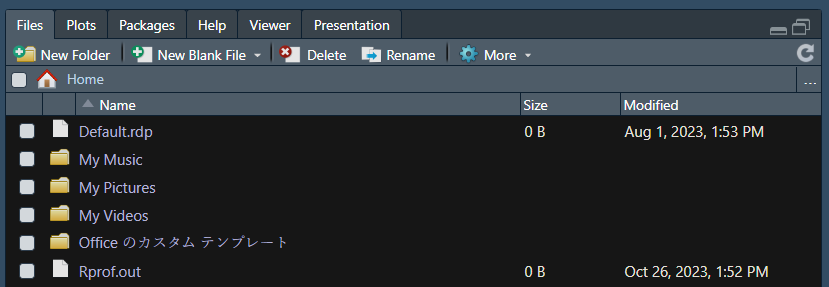
\includegraphics{././image/filestab.png}

}

\caption{図1:ワーキングディレクトリをfilesタブで確認する}

\end{figure}

このfilesタブでは,任意のフォルダに移動することができます.上図の右上,\ldots と記載されている部分をクリックするとウインドウが開きます.このウインドウ上で任意のフォルダに移動すれば,filesタブに示されるフォルダが変わります.ただし,表示するフォルダを変えるだけではワーキングディレクトリを変更することはできません.

filesタブに表示されたフォルダにワーキングディレクトリを設定するには,filesタブの右上,「More」から「Set
As Working Directory」を選択します.

\begin{figure}

{\centering 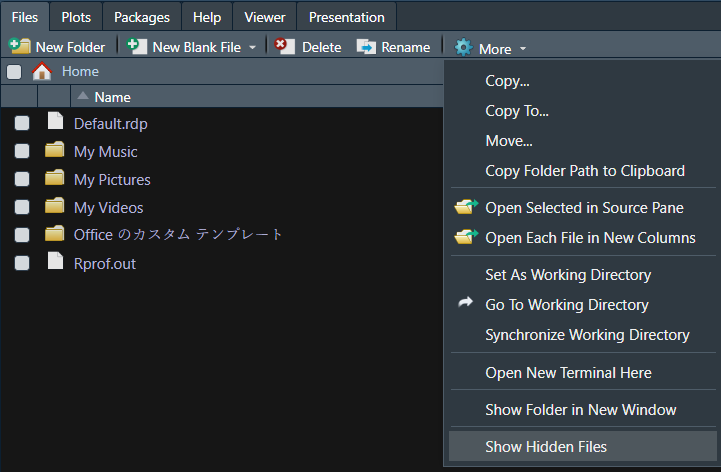
\includegraphics{././image/filestab_options.png}

}

\caption{図2:MoreのリストからSet As Working Directoryを選ぶ}

\end{figure}

ワーキングディレクトリを変更せずに,ワーキングディレクトリを表示し直す場合は,同じ「More」から「Go
To Working Directory」を選択します.

ワーキングディレクトリの変更は,上の「Session」からでも変更できます.

\begin{figure}

{\centering 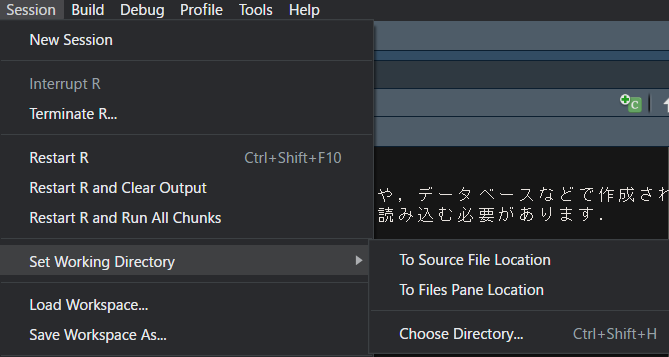
\includegraphics{././image/Session_SetWD.png}

}

\caption{図3:「Session」からワーキングディレクトリを変更する}

\end{figure}

デフォルトのワーキングディレクトリ(Rstudioを開いた時に設定されているワーキングディレクトリ)を変更する場合には,「Tools」→「Option」を選択し,「Default
working directory」に任意のフォルダを選択します.

\begin{figure}

{\centering 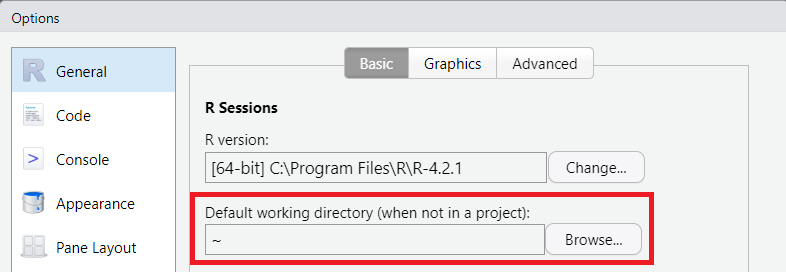
\includegraphics{././image/DefaultWD.png}

}

\caption{図4:デフォルトのワーキングディレクトリを変更する}

\end{figure}

\hypertarget{getwdux95a2ux6570ux3068setwdux95a2ux6570}{%
\subsection{getwd関数とsetwd関数}\label{getwdux95a2ux6570ux3068setwdux95a2ux6570}}

上記のように,Rstudioの機能を使えばワーキングディレクトリを簡単に変更することができます.ただし,データのフォルダ構造によっては,Rでの演算中にワーキングディレクトリを変更したい,といった場合もあります.

ワーキングディレクトリの確認と設定は,\textbf{getwd関数とsetwd関数}を用いて行うことができます.

\textbf{getwd関数}は現在のワーキングディレクトリを確認するための関数です.getwd関数は引数を取らず,実行すると現在のワーキングディレクトリのアドレスを文字列で返します.

\textbf{setwd関数}はワーキングディレクトリを変更するための関数です.setwd関数は\textbf{文字列のディレクトリのアドレス}を引数に取ります.setwd関数を実行すると,ワーキングディレクトリがアドレスで指定したフォルダに変更されます.

\begin{Shaded}
\begin{Highlighting}[]
\FunctionTok{getwd}\NormalTok{() }\CommentTok{\# ワーキングディレクトリを確認}
\FunctionTok{setwd}\NormalTok{(}\StringTok{"directory/name/as/character"}\NormalTok{) }\CommentTok{\# ワーキングディレクトリを変更}
\end{Highlighting}
\end{Shaded}

\hypertarget{ux7d76ux5bfeux30d1ux30b9ux3068ux76f8ux5bfeux30d1ux30b9}{%
\subsection{絶対パスと相対パス}\label{ux7d76ux5bfeux30d1ux30b9ux3068ux76f8ux5bfeux30d1ux30b9}}

ディレクトリを指定する際には,\textbf{ディレクトリのアドレス}を用います.Windowsでは,フォルダを開き,上のアドレスバーを右クリックすると,アドレスをテキストとしてコピーすることができます.この方法でコピーできるアドレスのことを\textbf{絶対パス}と呼びます.絶対パスは,ルートディレクトリ(大元のフォルダ)からそのフォルダまでのアドレスが全て記載されています.

\begin{figure}

{\centering 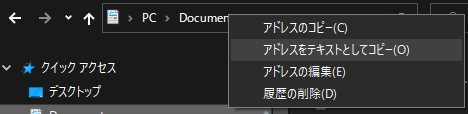
\includegraphics{././image/directory_address.png}

}

\caption{図5:ディレクトリのアドレス(Windowsの場合)}

\end{figure}

ディレクトリのアドレスには,\textbf{相対パス}と呼ばれるものもあります.相対パスは,現在のディレクトリの上や下といった,現在のディレクトリからの位置を相対的に表すものです.

setwd関数は,この絶対パス,相対パスのいずれも使用することができます.絶対パスの場合には,ルートからのすべてのアドレスを文字列で指定します.一方,相対パスの場合は,.(ピリオド)を用いて,現在のディレクトリからの位置を以下のように指定します.

\begin{itemize}
\tightlist
\item
  \textbf{「./」}は今のディレクトリのアドレスを示す記号
\item
  \textbf{「../」}は今のディレクトリの一つ上のディレクトリを示す記号
\end{itemize}

上の記号を用いて,一つ下にあるディレクトリは以下のように示すことができます.

\textbf{``./一つ下のフォルダ名''}

また,setwd関数は,下のフォルダであれば,そのフォルダまでのパスを記載するだけでもディレクトリを指定することができます.

\begin{Shaded}
\begin{Highlighting}[]
\FunctionTok{setwd}\NormalTok{(}\StringTok{"../"}\NormalTok{) }\CommentTok{\# 一つ上のフォルダにワーキングディレクトリを移動}
\FunctionTok{setwd}\NormalTok{(}\StringTok{"./NameF"}\NormalTok{) }\CommentTok{\# 一つ下の「NameF」というフォルダにワーキングディレクトリを移動}
\FunctionTok{setwd}\NormalTok{(}\StringTok{"NameF"}\NormalTok{) }\CommentTok{\# 上と同じ}
\FunctionTok{setwd}\NormalTok{(}\StringTok{"NameF/NameF2"}\NormalTok{) }\CommentTok{\# NameFフォルダ内のNameF2というフォルダに移動}
\end{Highlighting}
\end{Shaded}

\hypertarget{ux30c7ux30a3ux30ecux30afux30c8ux30eaux5185ux306eux30d5ux30a1ux30a4ux30ebux306eux78baux8a8d}{%
\section{ディレクトリ内のファイルの確認}\label{ux30c7ux30a3ux30ecux30afux30c8ux30eaux5185ux306eux30d5ux30a1ux30a4ux30ebux306eux78baux8a8d}}

ワーキングディレクトリ内のファイルやフォルダは,Rで開いたり,確認したりすることができます.\textbf{dir関数とlist.files関数}はワーキングディレクトリ内のファイル・フォルダを表示するための関数です.いずれもファイル・フォルダ名を文字列のベクターとして返します.\textbf{list.dirs関数}はワーキングディレクトリ以下にあるフォルダのアドレスを文字列のベクターとして返します.

\begin{Shaded}
\begin{Highlighting}[]
\FunctionTok{dir}\NormalTok{() }\CommentTok{\# ディレクトリ名とファイル名が返ってくる}
\FunctionTok{list.files}\NormalTok{() }\CommentTok{\# dir関数と同じ}
\FunctionTok{list.dirs}\NormalTok{() }\CommentTok{\# ディレクトリ名のみ返ってくる}
\end{Highlighting}
\end{Shaded}

\hypertarget{ux30d5ux30a9ux30ebux30c0ux3068ux30d5ux30a1ux30a4ux30ebux306eux4f5cux6210}{%
\section{フォルダとファイルの作成}\label{ux30d5ux30a9ux30ebux30c0ux3068ux30d5ux30a1ux30a4ux30ebux306eux4f5cux6210}}

現在のワーキングディレクトリにフォルダを作成する際には,\textbf{dir.create関数}を用います.dir.create関数は作成するフォルダ名の文字列を引数に取ります.ワーキングディレクトリ内にファイルを作成する関数はいくつもあります.単にファイルを作るのであればfile.create関数を,文字列をテキストで保存する場合にはcat関数を用います.

\begin{Shaded}
\begin{Highlighting}[]
\FunctionTok{dir.create}\NormalTok{(}\StringTok{"tmp"}\NormalTok{) }\CommentTok{\# 現在のワーキングディレクトリに「tmp」というフォルダを作成}
\FunctionTok{setwd}\NormalTok{(}\StringTok{"tmp"}\NormalTok{) }\CommentTok{\# 作成したフォルダにワーキングディレクトリを移動}
\FunctionTok{file.create}\NormalTok{(}\StringTok{"filename.txt"}\NormalTok{) }\CommentTok{\# 空のテキストファイルを作成}
\FunctionTok{cat}\NormalTok{(}\StringTok{"Hello world"}\NormalTok{, }\AttributeTok{file=}\StringTok{"helloworld.txt"}\NormalTok{) }\CommentTok{\# Hello worldと書き込まれたテキストファイルを作成}
\end{Highlighting}
\end{Shaded}

\hypertarget{ux30efux30fcux30afux30b9ux30daux30fcux30b9ux30a4ux30e1ux30fcux30b8.rdataux306eux4fddux5b58}{%
\section{ワークスペースイメージ(.Rdata)の保存}\label{ux30efux30fcux30afux30b9ux30daux30fcux30b9ux30a4ux30e1ux30fcux30b8.rdataux306eux4fddux5b58}}

\textbf{ワークスペース}とは,Rを実行している時に取り扱っているオブジェクトなどの環境のことです.RGUIやRstudioを閉じるときには,下の図のようなウインドウが表示され,ワークスペースのイメージを保存するかどうか尋ねられます.ワークスペースを保存すると,現在のワーキングディレクトリに「\textbf{.RData}」というファイルが作成されます.この.RDataがワークスペースのイメージです.

\begin{figure}

{\centering 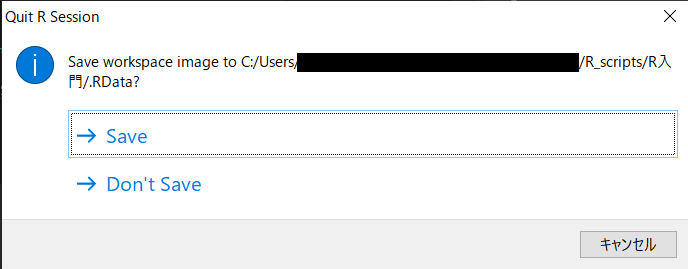
\includegraphics{././image/save_workspace.png}

}

\caption{図6:Rstudio終了時のワークスペース保存}

\end{figure}

.RDataファイルはRstudioを閉じるときだけでなく,Rstudioのメニューから「Session
→ Save Workspace
As\ldots」を選ぶことでも保存できます.また,\textbf{save.image関数}を用いても,.RDataファイルを作成することができます.

現在のワークスペースの情報は,Rstudio右上のパネルの「Environment」で確認できます.このパネルには,現在Rで取り扱っている変数(オブジェクト)の一覧を確認することができます.

\begin{figure}

{\centering 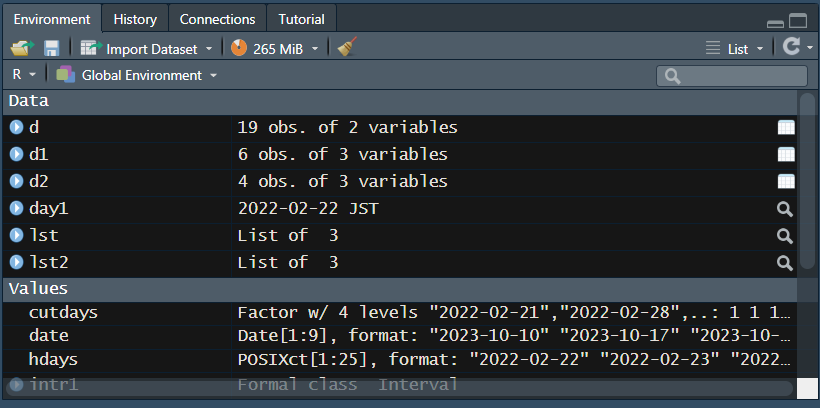
\includegraphics{././image/environment_pane.png}

}

\caption{図7:Environmentパネル}

\end{figure}

このパネルに表示されているのと同じ,オブジェクトのリストをR上で取得する場合には,\textbf{ls関数}を用います.

Rを閉じると,オブジェクトはメモリから削除されます.次にRStudioを起動したときには,デフォルトのワーキングディレクトリに存在する.RDataから自動的にワークスペースのイメージが読み込まれます.別途,.RDataファイルを指定してワークスペースを読み込む場合には,\textbf{load関数}を用います.load関数で.RDataファイルを読み込むことで,.RDataファイルを保存した際に使用していたオブジェクトがメモリ上に展開されます.

このように,ワークスペースを保存・読み込むことで,以前のデータ分析環境を読み込み,データ分析の続きを行うことができます.

\begin{Shaded}
\begin{Highlighting}[]
\FunctionTok{ls}\NormalTok{() }\CommentTok{\# 現在メモリ上にある全てのオブジェクトを表示}
\FunctionTok{save.image}\NormalTok{() }\CommentTok{\# ワークスペースのイメージを保存する}
\FunctionTok{load}\NormalTok{(}\StringTok{".Rdata"}\NormalTok{) }\CommentTok{\# ワークスペースのイメージを読み込む}
\end{Highlighting}
\end{Shaded}

\hypertarget{ux30aaux30d6ux30b8ux30a7ux30afux30c8ux306eux4fddux5b58ux3068ux8aadux307fux8fbcux307f}{%
\section{オブジェクトの保存と読み込み}\label{ux30aaux30d6ux30b8ux30a7ux30afux30c8ux306eux4fddux5b58ux3068ux8aadux307fux8fbcux307f}}

ワークスペース全体ではなく,個別のオブジェクトも,一時的に保存し,読み込むことができます.オブジェクトの保存と読み込みには,\textbf{save関数とload関数}を用います.

\textbf{save関数}はオブジェクトと文字列のファイル名の2つを引数に取り,オブジェクトを引数で指定したファイル名で保存する関数です.ファイル名は何でもよく,ファイルの拡張子にも特に指定はないのですが,\textbf{「.rda」}を拡張子としたファイル名とするのが一般的です.

保存したオブジェクトを読み込む関数が,\textbf{load関数}です.load関数はファイル名の文字列を引数に取り,save関数で保存した.rdaファイルを読み込みます.load関数で読み込むと,Rのワークスペースには保存したオブジェクトが現れます.

save・load関数と同様の関数として,dput関数とdget関数というものもありますが,こちらはそれほど利用されません.dput関数で保存したファイルはload関数で読み込めず,save関数で保存したファイルはdget関数で読み込めないため,dput関数でオブジェクトを保存した場合には,dget関数で読み込む必要があります.dget関数はオブジェクトを返す関数ですので,ワークスペースにオブジェクトが再現されるわけではありません.

\begin{Shaded}
\begin{Highlighting}[]
\NormalTok{x }\OtherTok{\textless{}{-}} \FunctionTok{c}\NormalTok{(}\DecValTok{1}\NormalTok{, }\DecValTok{2}\NormalTok{, }\DecValTok{3}\NormalTok{)}
\FunctionTok{save}\NormalTok{(x, }\AttributeTok{file =} \StringTok{"Robject.rda"}\NormalTok{) }\CommentTok{\# オブジェクトを保存}
\FunctionTok{rm}\NormalTok{(x) }\CommentTok{\# xを削除する}
\FunctionTok{load}\NormalTok{(}\StringTok{"Robject.rda"}\NormalTok{) }\CommentTok{\# オブジェクトの読み込み}
\NormalTok{x }\CommentTok{\# xが読み込まれている}

\FunctionTok{dput}\NormalTok{(x, }\StringTok{"Robject\_dput.rda"}\NormalTok{) }\CommentTok{\# オブジェクトを保存}
\FunctionTok{dget}\NormalTok{(}\StringTok{"Robject\_dput.rda"}\NormalTok{) }\CommentTok{\# オブジェクトが返ってくる}

\FunctionTok{dget}\NormalTok{(}\StringTok{"Robject.rda"}\NormalTok{) }\CommentTok{\# エラー.saveで保存するとdgetで読み込めない}
\FunctionTok{load}\NormalTok{(}\StringTok{"Robject\_dput.rda"}\NormalTok{) }\CommentTok{\# エラー.dputで保存するとloadで読み込めない}
\end{Highlighting}
\end{Shaded}

\hypertarget{ux30c7ux30fcux30bfux306eux8aadux307fux8fbcux307f}{%
\section{データの読み込み}\label{ux30c7ux30fcux30bfux306eux8aadux307fux8fbcux307f}}

\hypertarget{excelux304bux3089ux30c7ux30fcux30bfux3092ux8aadux307fux8fbcux3080ux53e4ux5178ux7684ux306aux65b9ux6cd5}{%
\subsection{Excelからデータを読み込む(古典的な方法)}\label{excelux304bux3089ux30c7ux30fcux30bfux3092ux8aadux307fux8fbcux3080ux53e4ux5178ux7684ux306aux65b9ux6cd5}}

統計を行うデータは,通常Excelのような表計算ソフトか,データベースで準備するのが一般的です.このようなデータをRで取り込む際には,一昔前までは\textbf{「テキストファイルに変換」}してから読み込むのが一般的でした.

最近ではライブラリを使用することでExcelやデータベースのファイルから直接データを読み込むことができますが,ライブラリなしのRではこのような読み込みはできません.ライブラリが使用できないときには,以下のような方法でExcelファイルをテキストで保存し,Rで読み込むことになります.

また,Web上に保存されているデータがテキストである場合も少なくありません.このような,Web上のテキストファイルの読み込みにも,以下に示すテキスト読み込みの方法を用いることができます.

\hypertarget{excelcsvux30bfux30d6ux5207ux308aux30c6ux30adux30b9ux30c8ux3078ux306eux5909ux63db}{%
\subsubsection{Excel:csv・タブ切りテキストへの変換}\label{excelcsvux30bfux30d6ux5207ux308aux30c6ux30adux30b9ux30c8ux3078ux306eux5909ux63db}}

まずは,Excelでのテキストファイルの変換について説明します.Rで読み込むテキストは,大きく分けると3種類です.

\begin{itemize}
\tightlist
\item
  \textbf{コンマ切りテキスト}(comma-separated values, \textbf{csv})
\item
  \textbf{タブ切りテキスト}(tab-separated values, \textbf{tsv})
\item
  スペース切りテキスト
\item
  固定幅テキスト
\end{itemize}

これらのうち,スペース切りテキストはデータにスペースが入っていると使えないので通常は避けられます.固定幅テキストはやや取り扱いにくいため,Excelからの変換には用いません.したがって,Excelファイルは主にコンマ切りテキストかタブ切りテキストに変換して,Rで読み込むことになります.

Excelファイルからコンマ切り・タブ切りテキストへの変換はExcel上で行います.Excelの「ファイル」メニューから「名前を付けて保存」を選択し,ファイル名の下のドロップダウンリストから「CSV
UTF-8 (コンマ区切り)(\emph{.csv)」もしくは「テキスト
(タブ区切り)(}.txt)」を選択します.拡張子である「.csv」や「.txt」は自動的に付与されます.

\begin{tcolorbox}[enhanced jigsaw, left=2mm, colframe=quarto-callout-tip-color-frame, opacitybacktitle=0.6, colbacktitle=quarto-callout-tip-color!10!white, opacityback=0, leftrule=.75mm, coltitle=black, bottomtitle=1mm, titlerule=0mm, bottomrule=.15mm, rightrule=.15mm, toptitle=1mm, breakable, arc=.35mm, toprule=.15mm, colback=white, title=\textcolor{quarto-callout-tip-color}{\faLightbulb}\hspace{0.5em}{エンコーディング}]

テキストには\textbf{エンコーディング}というものがあり,日本語テキストは\textbf{UTF-8,Shift-JIS(CP932),EUC-JP}のいずれかのエンコーディングを持ちます.エンコーディングが異なると文字化けを起こします.RのデフォルトのエンコーディングはUTF-8です.WindowsではShift-JISが用いられている場合があるため,エンコーディングに注意が必要となります.

\end{tcolorbox}

\begin{figure}

{\centering 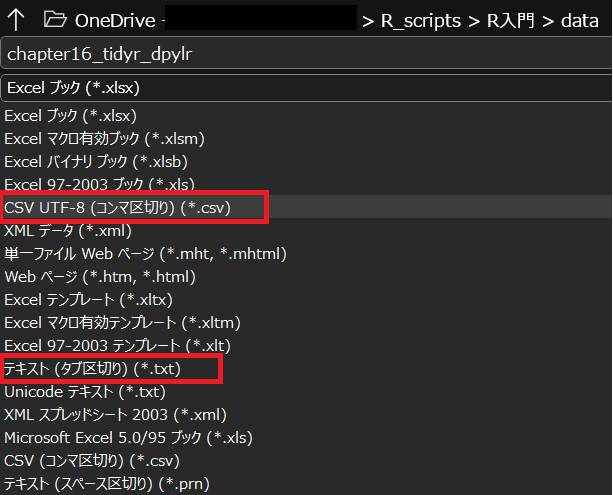
\includegraphics{././image/excel_changeformats.png}

}

\caption{図8:Excelでコンマ切り・タブ切りテキストを作成する}

\end{figure}

\begin{tcolorbox}[enhanced jigsaw, left=2mm, colframe=quarto-callout-tip-color-frame, opacitybacktitle=0.6, colbacktitle=quarto-callout-tip-color!10!white, opacityback=0, leftrule=.75mm, coltitle=black, bottomtitle=1mm, titlerule=0mm, bottomrule=.15mm, rightrule=.15mm, toptitle=1mm, breakable, arc=.35mm, toprule=.15mm, colback=white, title=\textcolor{quarto-callout-tip-color}{\faLightbulb}\hspace{0.5em}{Excelの空欄データ}]

Excelには「データをセルから消したのに何らかのデータが残る」という謎仕様があります.
空のExcelファイルを作成し(Book1),G7までを1で埋めます(Book2,下図9).数値をバックスペースで消して保存すると(Book3),何故かBook1よりBook3の方がファイルサイズが大きくなります(下図10).Rからテキスト変換したファイルを読み込むと,この「無いけど残っているデータ」を読み込んでしまうので,エラーが生じることがあります.データをdeleteで削除,もしくは右クリックから削除を選ぶと,この残ったデータを削除することができます.

\end{tcolorbox}

\begin{figure}

{\centering 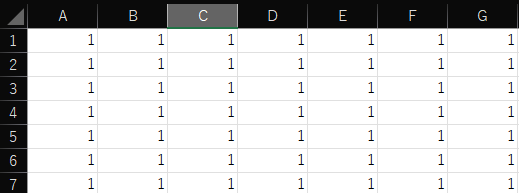
\includegraphics{././image/book2_excel.png}

}

\caption{図9:Excelのセルに1を入力し,バックスペースで削除する}

\end{figure}

\begin{figure}

{\centering 
\includegraphics{././image/filesize_excel.png}

}

\caption{図10:バックスペースで削除すると,ファイルサイズが増える}

\end{figure}

\hypertarget{scanux95a2ux6570}{%
\subsection{scan関数}\label{scanux95a2ux6570}}

まずは,1行のデータを読み込む場合について説明します.1行のデータであれば,\textbf{scan関数}を用いて読み込むことができます.scan関数の第一引数は文字列のファイル名です.ファイル名を指定するときには,必ず\textbf{拡張子を含めて記載します}.scan関数には,\textbf{「sep」}という引数を指定することができます.sepはデータ間の区切り文字を指定するものです.コンマ切りテキスト,CSVであれば\textbf{「sep
= ``,''」},タブ切りテキストであれば\textbf{「sep =
``\textbackslash t''」}を指定します.scan関数の返り値はベクターとなります.

ただし,whatという引数を設定すると,返り値をリストにすることができます.whatは空のリストを指定する引数で,リストの要素の個数に従い,scanで読み取った結果が代入されます.代入の順番は,1つ目がリストの1要素目,2つ目がリストの2要素目\ldots となります.リストの長さより多い要素は再びリストの1要素目に代入されます.

\begin{Shaded}
\begin{Highlighting}[]
\FunctionTok{scan}\NormalTok{(}\StringTok{"./data/scansample.txt"}\NormalTok{, }\AttributeTok{sep =} \StringTok{","}\NormalTok{) }\CommentTok{\# コンマ切りテキストを読み込む}
\end{Highlighting}
\end{Shaded}

\begin{verbatim}
[1] 1 2 3 4 5 6 7 8
\end{verbatim}

\begin{Shaded}
\begin{Highlighting}[]
\FunctionTok{scan}\NormalTok{(}\StringTok{"./data/scansample.txt"}\NormalTok{, }\AttributeTok{sep =} \StringTok{","}\NormalTok{, }\AttributeTok{what =} \FunctionTok{list}\NormalTok{(}\StringTok{""}\NormalTok{, }\StringTok{""}\NormalTok{)) }\CommentTok{\# 出力をリストにする}
\end{Highlighting}
\end{Shaded}

\begin{verbatim}
[[1]]
[1] "1" "3" "5" "7"

[[2]]
[1] "2" "4" "6" "8"
\end{verbatim}

\hypertarget{read.tableux95a2ux6570}{%
\subsection{read.table関数}\label{read.tableux95a2ux6570}}

Excelから読み込む表は,通常行と列を持つ,テーブルの形をしています.テキストに変換したExcelの表をデータフレームとして読み込む関数が\textbf{read.table関数}です.read.table関数は第一引数にテキストファイルのファイル名を取ります.scan関数と同様に,ファイル名には拡張子を含める必要があります.

read.table関数はscan関数と同じく,\textbf{「sep」}引数を取ります.sep引数には,コンマ切りテキスト,CSVであれば\textbf{「sep
= ``,''」},タブ切りテキストであれば\textbf{「sep =
``\textbackslash t''」}を指定します.

read.table関数は,\textbf{「header」}という引数を取ります.この引数にTRUEを指定すると(「header
= T」),読み込むテキストの1行目を列名として,データを読み込みます.

read.table関数でよく用いられる引数はファイル名,sep,headerの3つですが,その他たくさんの引数を取ることができます.read.table関数の引数の一覧を以下の表1に示します.

\begin{longtable}[]{@{}
  >{\raggedright\arraybackslash}p{(\columnwidth - 6\tabcolsep) * \real{0.1868}}
  >{\raggedright\arraybackslash}p{(\columnwidth - 6\tabcolsep) * \real{0.1648}}
  >{\raggedright\arraybackslash}p{(\columnwidth - 6\tabcolsep) * \real{0.4505}}
  >{\raggedright\arraybackslash}p{(\columnwidth - 6\tabcolsep) * \real{0.1978}}@{}}
\caption{表1:read.table関数の引数}\tabularnewline
\toprule()
\begin{minipage}[b]{\linewidth}\raggedright
引数
\end{minipage} & \begin{minipage}[b]{\linewidth}\raggedright
データ型
\end{minipage} & \begin{minipage}[b]{\linewidth}\raggedright
意味
\end{minipage} & \begin{minipage}[b]{\linewidth}\raggedright
デフォルト値
\end{minipage} \\
\midrule()
\endfirsthead
\toprule()
\begin{minipage}[b]{\linewidth}\raggedright
引数
\end{minipage} & \begin{minipage}[b]{\linewidth}\raggedright
データ型
\end{minipage} & \begin{minipage}[b]{\linewidth}\raggedright
意味
\end{minipage} & \begin{minipage}[b]{\linewidth}\raggedright
デフォルト値
\end{minipage} \\
\midrule()
\endhead
file & 文字列 & ファイル名 & ー \\
header & 論理型 & 1行目を列名とするか & FALSE \\
sep & 文字列 & 区切り文字(コンマやタブ) & ー \\
quote & 文字列 & 文字列が囲まれている文字(``など) & ``"''' \\
dec & 文字列 & 小数点の文字 & ``.'' \\
numerals & 文字列 & 文字列を数値に変換するときの正確性 & ー \\
row.names & 文字列ベクター & 行名 & ー \\
col.names & 文字列ベクター & 列名 & ー \\
as.is & 文字列 & 文字列を因子に変えるときのルール & !stringAsFactors \\
tryLogical & 論理型 & TRUEなどを論理型に変換するか & TRUE \\
na.strings & 文字列 & NAとして取り扱う文字列 & ``NA'' \\
colClasses & 文字列 & 列のクラスを指定 & NA \\
nrows & 数値 & 読み込む行数 & -1 \\
skip & 数値 & 読み込まない行数 & 0 \\
check.names & 論理型 & 列名をチェックするか & TRUE \\
fill & 論理型 & 空きになっている要素をスペースで埋めるか &
!blank.lines.skip \\
strip.white & 論理型 & スペースを取り除くか & FALSE \\
blank.lines.skip & 論理型 & 空行をスキップするか & TRUE \\
comment.char & 文字列 & コメントの開始文字 & ``\#'' \\
allowEscapes & 論理型 & エスケープ記号を変換するか & FALSE \\
flush & 論理型 & 1行1データかどうか & FALSE \\
stringAsFactors & 論理型 & 文字列を因子に自動変換するか & FALSE \\
fileEncoding & 文字列 & エンコーディングの指定 & ``\,'' \\
encoding & 文字列 & エンコーディング(変更はしない) & ``unknown'' \\
text & 文字列 & fileから読み込まず,直接データを入力 & ー \\
skipNul & 論理型 & 空データをスキップするか & FALSE \\
\bottomrule()
\end{longtable}

\hypertarget{read.csvux95a2ux6570read.delimux95a2ux6570}{%
\subsection{read.csv関数,read.delim関数}\label{read.csvux95a2ux6570read.delimux95a2ux6570}}

read.table関数の仲間には,csvの読み込み用の\textbf{read.csv関数},タブ切りテキスト読み込み用の\textbf{read.delim関数},固定幅テキストの読み込み用の\textbf{read.fwf関数}が準備されています.read.csv関数はsep引数にコンマ,read.delim関数はsep引数にタブがデフォルト値として設定されており,sep引数を記入することなくデータを読み込むことができます.

\begin{tcolorbox}[enhanced jigsaw, left=2mm, colframe=quarto-callout-tip-color-frame, opacitybacktitle=0.6, colbacktitle=quarto-callout-tip-color!10!white, opacityback=0, leftrule=.75mm, coltitle=black, bottomtitle=1mm, titlerule=0mm, bottomrule=.15mm, rightrule=.15mm, toptitle=1mm, breakable, arc=.35mm, toprule=.15mm, colback=white, title=\textcolor{quarto-callout-tip-color}{\faLightbulb}\hspace{0.5em}{ヨーロッパで準備されたファイルのデータ読み込み}]

ヨーロッパではコンマ(,)をセミコロン(;),小数点(ピリオド
.)をコンマ(,)と記載するため,通常のread.csv関数,read.delim関数ではテキストファイルをまともに読み込むことができません.ヨーロッパで生成されるテキストファイルには,専用の関数(read.csv2,read.delim2)が設けられています.

\end{tcolorbox}

\hypertarget{stringasfactorsux3068fileencoding}{%
\subsubsection{stringAsFactorsとfileEncoding}\label{stringasfactorsux3068fileencoding}}

read.table関数の「stringAsFactors」という引数は,昔はTRUEがデフォルトとされており,read.table関数で読み込んだ文字列はすべて因子に変換されていました.Rのバージョン4.0.0よりstringAsFactorsのデフォルト値がFALSEに変更されたため,現在のread.table関数では,文字列は文字列のまま読み込まれます.WindowsではテキストファイルのエンコーディングがShift
JISになっている場合がありますので,「fileEncoding =
``CP932''」を引数に指定しないと読み込めないことがあります.エンコーディングがUTF-8であれば,fileEncodingを指定する必要はありません.

\begin{Shaded}
\begin{Highlighting}[]
\FunctionTok{read.table}\NormalTok{(}\StringTok{"filename.txt"}\NormalTok{, }\AttributeTok{sep=}\StringTok{"}\SpecialCharTok{\textbackslash{}t}\StringTok{"}\NormalTok{, }\AttributeTok{header=}\NormalTok{T)}
\FunctionTok{read.table}\NormalTok{(}\StringTok{"filename.txt"}\NormalTok{, }\AttributeTok{sep=}\StringTok{"}\SpecialCharTok{\textbackslash{}t}\StringTok{"}\NormalTok{, }\AttributeTok{header=}\NormalTok{T, }\AttributeTok{stringAsFactors =}\NormalTok{ T)}
\FunctionTok{read.csv}\NormalTok{(}\StringTok{"filename.csv"}\NormalTok{)}
\FunctionTok{read.csv2}\NormalTok{(}\StringTok{"filename.csv"}\NormalTok{) }\CommentTok{\# ヨーロッパ仕様}
\FunctionTok{read.delim}\NormalTok{(}\StringTok{"filename.tsv"}\NormalTok{)}
\FunctionTok{read.delim2}\NormalTok{(}\StringTok{"filename.tsv"}\NormalTok{) }\CommentTok{\# ヨーロッパ仕様}

\FunctionTok{read.fwf}\NormalTok{(}\StringTok{"filename.txt"}\NormalTok{) }\CommentTok{\# 固定幅テキスト}
\end{Highlighting}
\end{Shaded}

\hypertarget{ux30afux30eaux30c3ux30d7ux30dcux30fcux30c9ux304bux3089ux306eux8aadux307fux8fbcux307f}{%
\subsection{クリップボードからの読み込み}\label{ux30afux30eaux30c3ux30d7ux30dcux30fcux30c9ux304bux3089ux306eux8aadux307fux8fbcux307f}}

Rでは,コピーしたテキストをクリップボードから読み込むこともできます.Ctrl+Cなどでコピーしたテキストを読み込む場合には,read.table関数の引数に''clipboard''を指定します.

\begin{Shaded}
\begin{Highlighting}[]
\FunctionTok{read.table}\NormalTok{(}\StringTok{"clipboard"}\NormalTok{)}
\end{Highlighting}
\end{Shaded}

\hypertarget{ux30c7ux30fcux30bfux306eux66f8ux304dux51faux3057}{%
\section{データの書き出し}\label{ux30c7ux30fcux30bfux306eux66f8ux304dux51faux3057}}

Rからのデータの書き出しは,通常テキストファイルで行います.Excelファイルに直接書き出すこともできなくは無いのですが(\href{https://cran.r-project.org/web/packages/xlsx/index.html}{xlsxパッケージ}を利用する),それほど一般的ではありません.データの書き出しに用いられる関数には,\textbf{write関数},\textbf{write.table関数}などがあります.

\hypertarget{writecatux95a2ux6570}{%
\subsection{write・cat関数}\label{writecatux95a2ux6570}}

ベクターや行列などのデータの書き出しには,write関数・cat関数を用います.write関数はcat関数のラッパーで,2つの関数の間には大きな差はありません.cat関数はオブジェクトをコンソールに表示するために用いられますが,ファイルを出力する事もできます.print関数を用いてもコンソールへ表示することはできますが,ファイルを保存することはできません.

cat関数,write関数は,オブジェクトとファイル名を引数に取ります.共にsep引数で区切り文字を指定することができます.

\begin{Shaded}
\begin{Highlighting}[]
\NormalTok{vec }\OtherTok{\textless{}{-}} \FunctionTok{c}\NormalTok{(}\DecValTok{1}\NormalTok{, }\DecValTok{2}\NormalTok{, }\DecValTok{3}\NormalTok{)}
\FunctionTok{cat}\NormalTok{(vec) }\CommentTok{\# consoleにvecを表示}
\FunctionTok{write}\NormalTok{(vec) }\CommentTok{\# cat関数と同じ}

\FunctionTok{print}\NormalTok{(vec) }\CommentTok{\# print関数でも表示できる}
\end{Highlighting}
\end{Shaded}

\begin{Shaded}
\begin{Highlighting}[]
\FunctionTok{cat}\NormalTok{(vec, }\AttributeTok{file=}\StringTok{"cat.txt"}\NormalTok{)}
\FunctionTok{write}\NormalTok{(vec, }\AttributeTok{file=}\StringTok{"vector.txt"}\NormalTok{, }\AttributeTok{sep=}\StringTok{"}\SpecialCharTok{\textbackslash{}t}\StringTok{"}\NormalTok{)}
\FunctionTok{print}\NormalTok{(vec, }\StringTok{"print.txt"}\NormalTok{) }\CommentTok{\# エラー}
\end{Highlighting}
\end{Shaded}

\hypertarget{write.tableux95a2ux6570}{%
\subsection{write.table関数}\label{write.tableux95a2ux6570}}

Rでは,データ処理の多くはデータフレームを用いて行います.統計結果もデータフレームにまとめて取り扱う場合が多いです.

テキストファイルをデータフレームとして取り込むread.table関数と逆に,データフレームをテキストファイルとして書き出す関数が\textbf{write.table関数}です.

write.table関数はデータフレームとファイル名を引数に取り,データフレームをそのファイル名のテキストファイルとして書き出します.

write.table関数の代表的な引数は,\textbf{sep,col.names,row.names,quote}の4つです.sepはread.table関数と同じく区切り文字を指定する引数です.col.namesとrow.namesは論理型を取り,TRUEであれば列名・行名を保存し,FALSEであれば列名・行名を省いて保存します.quoteも論理型を取り,文字列・因子をダブルクオーテーションで囲むするかどうかを指定します.

read.table関数にread.csv関数があったように,write.table関数にはCSV用の\textbf{write.csv関数}があります.write.csv関数はsepのデフォルト値にコンマが設定されています.ヨーロッパ仕様のwrite.csv2関数もありますが,日本で使用することはまれです.

\begin{Shaded}
\begin{Highlighting}[]
\FunctionTok{write.table}\NormalTok{(df\_obj, }\StringTok{"filename.txt"}\NormalTok{, }\AttributeTok{sep =} \StringTok{"}\SpecialCharTok{\textbackslash{}t}\StringTok{"}\NormalTok{)}

\CommentTok{\# 列名あり,行名なし,ダブルクオーテーションなしで保存}
\FunctionTok{write.table}\NormalTok{(df\_obj, }\StringTok{"filename.txt"}\NormalTok{, }\AttributeTok{sep =} \StringTok{"}\SpecialCharTok{\textbackslash{}t}\StringTok{"}\NormalTok{, }\AttributeTok{col.names =}\NormalTok{ T, }\AttributeTok{row.names =}\NormalTok{ F, }\AttributeTok{quote =}\NormalTok{ F) }

\FunctionTok{write.csv}\NormalTok{(df\_obj, }\StringTok{"filename.csv"}\NormalTok{)}
\FunctionTok{write.csv2}\NormalTok{(df\_obj, }\StringTok{"filename.csv"}\NormalTok{) }\CommentTok{\#  ヨーロッパ仕様}
\end{Highlighting}
\end{Shaded}

\hypertarget{readr}{%
\section{readr}\label{readr}}

RのデフォルトのI/Oは上記の通りですが,read.table関数,write.table関数を用いると,指定する引数が多かったり,列のデータ型が思うように設定されなかったりすることがよく起こります.また,デフォルトの関数群は実行速度が遅く,大きなデータを取り扱う場合にはとても時間がかかる,という問題もあります.

これらの不都合を解決するI/Oに関するライブラリが\textbf{readrパッケージ}です.readrパッケージは,Rのデフォルトの関数名のピリオドをアンダースコア(\_)に変換した関数群を備えており,列の型をうまく設定してくれる仕組みを備えています.また,デフォルトの関数よりも実行速度が速いため,大きなデータを取り扱う場合には,readrの関数群を用いたほうが良いでしょう.

readrパッケージはtidyverseを構成するライブラリの一つであり,インストール・ロードはtidyverseライブラリのインストール・ロードと同時に行うことができます.

\begin{Shaded}
\begin{Highlighting}[]
\NormalTok{pacman}\SpecialCharTok{::}\FunctionTok{p\_load}\NormalTok{(tidyverse)}
\end{Highlighting}
\end{Shaded}

\hypertarget{readrux30c6ux30adux30b9ux30c8ux30c7ux30fcux30bfux306eux8aadux307fux8fbcux307f}{%
\subsection{readr:テキストデータの読み込み}\label{readrux30c6ux30adux30b9ux30c8ux30c7ux30fcux30bfux306eux8aadux307fux8fbcux307f}}

readrでのテキストデータの読み込みには,\textbf{read\_table関数}を用います.read\_table関数の使い方はread.table関数とほぼ同じです.read.table関数と同じく,read\_table関数も区切り文字をsep引数で設定します.read\_table関数のデフォルトの区切り文字はスペースですので,sepを設定しない場合にはスペース切りテキストの読み込みに対応しています.読み込まれたファイルは,\textbf{tibble}というデータ型の,データフレームに変換されます.

コンマ切りテキスト(CSV)の読み込みには,read\_csvが,タブ切りテキスト(TSV)の読み込みには\textbf{read\_csv関数とread\_tsv関数}が準備されています.これらの他に,ヨーロッパ仕様のCSVを読み込むread\_csv2関数,\textbar を区切り文字とするread\_delim関数,固定幅テキストの読み込みを行うread\_fwf関数などがあります.

readrパッケージの読み込み関数は圧縮ファイルの読み込みにも対応しており,gzip(.gz),bzip2(.bz2),lzma(.xz),zip(.zip)などの圧縮ファイルを直接読み込むことができます.また,インターネットからテキストファイルを直接読み込むことができます.インターネットから直接読み込む場合には,テキストファイルが保存されているwebアドレス(http://,
https://, ftp:// など)をファイル名として設定します.

\begin{Shaded}
\begin{Highlighting}[]
\FunctionTok{read\_table}\NormalTok{(}\StringTok{"filename.txt"}\NormalTok{) }\CommentTok{\# sep=" "(スペース切り)がデフォルト}
\FunctionTok{read\_delim}\NormalTok{(}\StringTok{"filename.txt"}\NormalTok{) }\CommentTok{\# sep="|"がデフォルト}
\FunctionTok{read\_csv}\NormalTok{(}\StringTok{"filename.csv"}\NormalTok{) }\CommentTok{\# コンマ切りテキスト}
\FunctionTok{read\_csv2}\NormalTok{(}\StringTok{"filename.csv"}\NormalTok{) }\CommentTok{\# ヨーロッパ仕様}
\FunctionTok{read\_tsv}\NormalTok{(}\StringTok{"filename.tsv"}\NormalTok{) }\CommentTok{\# タブ切りテキスト}
\FunctionTok{read\_fwf}\NormalTok{(}\StringTok{"filename.txt"}\NormalTok{) }\CommentTok{\# 固定幅テキスト}

\FunctionTok{read\_delim}\NormalTok{(}\FunctionTok{clipboard}\NormalTok{()) }\CommentTok{\# クリップボードの読み込み}

\FunctionTok{read\_table}\NormalTok{(}\StringTok{"filename.zip"}\NormalTok{) }\CommentTok{\# zipファイルも直接読み込める}
\end{Highlighting}
\end{Shaded}

\hypertarget{tibble}{%
\subsection{tibble}\label{tibble}}

readrの読み込み関数は,読み込んだデータを\textbf{tibble}というデータ型に変換します.このtibbleは概ねデータフレームと同じで,取り扱いもデータフレームと同様に行うことができます.

tibbleはtibble関数で,データフレームと同じように作成することができます.また,as\_tibble関数を用いることで,行列や通常のデータフレームをtibbleに変換することができます.

readrに限らず,tidyverseのライブラリ群はデータフレームをこのtibbleに変換するように設定されているものが多いです.tibbleのデータフレームは,表示した時に列のデータ型を表示する,10行以上の行は省略する,列も省略する等の特徴があります.tibbleについては,tidyr・dplyr,purrrパッケージに関する章で詳しく説明します.

\begin{Shaded}
\begin{Highlighting}[]
\NormalTok{pacman}\SpecialCharTok{::}\FunctionTok{p\_load}\NormalTok{(tidyverse)}

\FunctionTok{tibble}\NormalTok{(}\AttributeTok{x =} \DecValTok{1}\SpecialCharTok{:}\DecValTok{3}\NormalTok{, }\AttributeTok{y =} \FunctionTok{c}\NormalTok{(}\StringTok{"a"}\NormalTok{, }\StringTok{"b"}\NormalTok{, }\StringTok{"c"}\NormalTok{), }\AttributeTok{z =} \FunctionTok{c}\NormalTok{(T, F, T))}
\end{Highlighting}
\end{Shaded}

\begin{verbatim}
# A tibble: 3 x 3
      x y     z    
  <int> <chr> <lgl>
1     1 a     TRUE 
2     2 b     FALSE
3     3 c     TRUE 
\end{verbatim}

\begin{Shaded}
\begin{Highlighting}[]
\FunctionTok{as\_tibble}\NormalTok{(iris)}
\end{Highlighting}
\end{Shaded}

\begin{verbatim}
# A tibble: 150 x 5
   Sepal.Length Sepal.Width Petal.Length Petal.Width Species
          <dbl>       <dbl>        <dbl>       <dbl> <fct>  
 1          5.1         3.5          1.4         0.2 setosa 
 2          4.9         3            1.4         0.2 setosa 
 3          4.7         3.2          1.3         0.2 setosa 
 4          4.6         3.1          1.5         0.2 setosa 
 5          5           3.6          1.4         0.2 setosa 
 6          5.4         3.9          1.7         0.4 setosa 
 7          4.6         3.4          1.4         0.3 setosa 
 8          5           3.4          1.5         0.2 setosa 
 9          4.4         2.9          1.4         0.2 setosa 
10          4.9         3.1          1.5         0.1 setosa 
# i 140 more rows
\end{verbatim}

\hypertarget{readrux30c6ux30adux30b9ux30c8ux30d5ux30a1ux30a4ux30ebux306eux66f8ux304dux51faux3057}{%
\subsection{readr:テキストファイルの書き出し}\label{readrux30c6ux30adux30b9ux30c8ux30d5ux30a1ux30a4ux30ebux306eux66f8ux304dux51faux3057}}

readrパッケージにはwrite.table関数に当たる,テキスト書き出しの関数を備えています.readrが備えている関数は,データフレームをCSVとして保存する\textbf{write\_csv関数},タブ切りテキストとして保存する\textbf{write\_tsv関数},スペース切りテキストとして保存する\textbf{write\_delim関数}があります.write\_table関数というものは設定されていないので,基本的にはCSVかタブ切りテキストとして保存することが想定されているようです.

read\_table関数と同様に,write\_関数もテキストの圧縮ファイルの保存に対応しています.対応している圧縮ファイルはgzip(.gz),bzip2(.bz2),lzma(.xz)です.

\begin{Shaded}
\begin{Highlighting}[]
\FunctionTok{write\_csv}\NormalTok{(x, }\StringTok{"filename.csv"}\NormalTok{) }\CommentTok{\# コンマ切り}
\FunctionTok{write\_tsv}\NormalTok{(x, }\StringTok{"filename.tsv"}\NormalTok{) }\CommentTok{\# タブ切り}
\FunctionTok{write\_delim}\NormalTok{(x, }\StringTok{"filename.txt"}\NormalTok{) }\CommentTok{\# スペース切り}
\FunctionTok{write\_csv2}\NormalTok{(x, }\StringTok{"filename.csv"}\NormalTok{) }\CommentTok{\# ヨーロッパ仕様}

\FunctionTok{write\_csv}\NormalTok{(x, }\StringTok{"filename.gz"}\NormalTok{) }\CommentTok{\# gzipで圧縮して出力}
\FunctionTok{write\_csv}\NormalTok{(x, }\StringTok{"filename.bz2"}\NormalTok{) }\CommentTok{\# bzip2で圧縮して出力}
\FunctionTok{write\_csv}\NormalTok{(x, }\StringTok{"filename.xz"}\NormalTok{) }\CommentTok{\# lzmaで圧縮して出力}
\end{Highlighting}
\end{Shaded}

\hypertarget{readxl}{%
\section{readxl}\label{readxl}}

R使いは上記のように,昔からExcelをテキストファイルに変換してはRに読み込むというステップを踏み続けてきました.このExcelからテキストへの変換の手間を無くすライブラリが\textbf{readxl}パッケージです.

readxlパッケージもtidyverseと同じく,\href{https://posit.co/}{Posit
Software}が開発しているライブラリですが,tidyverseには含まれていません.tidyverseとは別に,readxlパッケージを独立に読み込む必要があります.

readxlパッケージで使用する関数は,ほぼ\textbf{read\_excel関数}だけです.read\_excel関数は,.xlsおよび.xlsxファイルの読み込みに対応しており,ファイル名で指定したExcelファイルからテーブルをtibbleとして読み込みます.read\_excel関数にはsheetという引数を設定することができます.read\_excel関数はsheetに設定した番号(もしくはシート名)のシートを読み込みます.

readxlパッケージにはread\_excel関数以外に,Excelファイルのメタデータ読み込みのための関数などを備えています.

\begin{Shaded}
\begin{Highlighting}[]
\NormalTok{pacman}\SpecialCharTok{::}\FunctionTok{p\_load}\NormalTok{(readxl)}
\FunctionTok{read\_excel}\NormalTok{(}\StringTok{"filename.xlsx"}\NormalTok{, }\AttributeTok{sheet =} \DecValTok{1}\NormalTok{) }\CommentTok{\# read\_xlsxが読み込まれる}
\FunctionTok{read\_excel}\NormalTok{(}\StringTok{"filename.xls"}\NormalTok{, }\AttributeTok{sheet =} \DecValTok{1}\NormalTok{) }\CommentTok{\# read\_xlsが読み込まれる}
\end{Highlighting}
\end{Shaded}

Excelには昔使用されていたファイルである.xlsファイルと,Excel2007から使われている.xlsxファイルがあります.

.xlsファイルはバイナリファイルで,内部的には1と0でデータが表現されています.

.xlsxファイルは実際にはzipファイルで,xmlというフォーマットで記載されたデータがzipファイルのフォルダ内に含まれています..xlsxファイルは拡張子を.zipに書き換えるとzipファイルとして解凍することができ,中身を確認することができます.

.xlsと.xlsxは全然違うファイルですが,read\_excel関数は拡張子によって.xlsを読み込むread\_xls関数と.xlsxを読み込むread\_xlsx関数を切り替えて呼び出しています.

\hypertarget{ux305dux306eux4ed6ux306eux30c7ux30fcux30bfux8aadux307fux8fbcux307fux30e9ux30a4ux30d6ux30e9ux30ea}{%
\subsubsection{その他のデータ読み込みライブラリ}\label{ux305dux306eux4ed6ux306eux30c7ux30fcux30bfux8aadux307fux8fbcux307fux30e9ux30a4ux30d6ux30e9ux30ea}}

\href{https://posit.co/}{Posit
Software}はreadxlの他にも,多数のデータ読み込み用ライブラリを開発しています.以下に示したライブラリを利用することで,様々なデータ型のファイルをRで読み込み,統計に用いることができます.

\begin{itemize}
\tightlist
\item
  \href{https://googlesheets4.tidyverse.org/}{googlesheet4}:Googleスプレッドシートの読み込み
\item
  \href{https://haven.tidyverse.org/}{haven}:SAS,SPSS,Stataファイルの読み込み
\item
  \href{https://cran.r-project.org/web/packages/jsonlite/vignettes/json-aaquickstart.html}{jsonlite}:jsonファイルの読み込み
\item
  \href{https://httr.r-lib.org/}{httr}:Webからの読み込み
\item
  \href{https://rvest.tidyverse.org/}{rvest}:スクレイピング用ライブラリ
\item
  \href{https://dbi.r-dbi.org/}{DBI}:データベースの読み込み
\end{itemize}

\hypertarget{data.table}{%
\section{data.table}\label{data.table}}

近年のデータサイエンスでは,100万~数千億程度のデータを取り扱うこともあります.個人のPCでRを使ってこのような超大規模のデータを取り扱うのは現実的ではありませんが,数万~数十万行ぐらいのデータをPCで取り扱う場合は増えてきています.例えば,生物分野では\href{https://ja.wikipedia.org/wiki/\%E3\%83\%9E\%E3\%82\%A4\%E3\%82\%AF\%E3\%83\%AD\%E3\%82\%A2\%E3\%83\%AC\%E3\%82\%A4}{マイクロアレイ}や\href{https://jp.illumina.com/content/dam/illumina-marketing/apac/japan/documents/pdf/primer_illumina_sequencing_introduction-j.pdf}{高速シークエンサー}のデータは数万~数十万行で,分析を個人が,自分のPCで取り扱うこともあるかと思います.自分でマイクロアレイやシークエンサーを使ってデータを出さなくても,\href{https://www.ncbi.nlm.nih.gov/gds}{GEO
Dataset}などからデータを取得して,解析してみるのも昔よりは一般的に行われています.

このような,超巨大データを取り扱う場合,R謹製のread.table関数では手に余りますし,read\_table関数を用いても,読み込んだ後のデータ処理が重く,取り扱いに苦労します.このような大規模データの読み込みに特化したライブラリが,\textbf{data.tableパッケージ}です.

\href{https://cran.r-project.org/web/packages/data.table/vignettes/datatable-intro.html}{data.tableパッケージ}は,大規模データを読み込み,Rで高速に利用できるよう設計されたライブラリです.

data.tableパッケージでデータを読み込むときには,\textbf{fread関数}を用います.fread関数はhtmlからの読み込みにも対応しています.読み込んだデータはdata.tableクラスのオブジェクトとなります.

\begin{Shaded}
\begin{Highlighting}[]
\NormalTok{pacman}\SpecialCharTok{::}\FunctionTok{p\_load}\NormalTok{(data.table)}

\CommentTok{\# flights14(NYのフライトデータ,25万行11列)をinputとする}
\NormalTok{input }\OtherTok{\textless{}{-}} \StringTok{"https://raw.githubusercontent.com/Rdatatable/data.table/master/vignettes/flights14.csv"}

\CommentTok{\# freadで読み込む}
\NormalTok{flights }\OtherTok{\textless{}{-}} \FunctionTok{fread}\NormalTok{(input) }\CommentTok{\# 219MBのデータ読み込み}
\FunctionTok{class}\NormalTok{(flights)}
\FunctionTok{dim}\NormalTok{(flights)}
\end{Highlighting}
\end{Shaded}

data.tableの取り扱いの方法はほぼデータフレームと同じです.data.tableはインデックスからデータの要約ができる機構を備えています.ただし,後の章で説明するtidyr・dplyrの関数も適用できますので,データの要約はtidyr・dplyrで行ってもよいでしょう.

\begin{Shaded}
\begin{Highlighting}[]
\NormalTok{flights[}\DecValTok{5}\NormalTok{, }\DecValTok{1}\NormalTok{] }\CommentTok{\# 通常のインデックスに対応}
\NormalTok{flights[}\DecValTok{1}\SpecialCharTok{:}\DecValTok{5}\NormalTok{] }\CommentTok{\# 行列を指定しない場合は,行のインデックスになる}
\NormalTok{flights[}\DecValTok{1}\SpecialCharTok{:}\DecValTok{5}\NormalTok{, }\DecValTok{2}\SpecialCharTok{:}\DecValTok{5}\NormalTok{] }\CommentTok{\# ベクターでの読み出しにも対応}

\FunctionTok{head}\NormalTok{(flights[origin }\SpecialCharTok{==} \StringTok{"JFK"}\NormalTok{, ]) }\CommentTok{\# originがJFKの行を選択}
\FunctionTok{head}\NormalTok{(flights[, .(month, day)]) }\CommentTok{\# monthとdayの列を選択}
\FunctionTok{head}\NormalTok{(flights}\SpecialCharTok{$}\NormalTok{origin) }\CommentTok{\# originの列を抽出}
\end{Highlighting}
\end{Shaded}

\begin{quote}
data.tableが使われ始めた頃は,data.tableオブジェクトの取り扱い方がデータフレームとは大きく異なっており,かなりとっつきにくかったのですが,現在ではデータフレームとほぼ同じ取り扱いができるようになっています.
\end{quote}

\bookmarksetup{startatroot}

\hypertarget{ux30c7ux30fcux30bfux30bbux30c3ux30c8}{%
\chapter{データセット}\label{ux30c7ux30fcux30bfux30bbux30c3ux30c8}}

Rには、データ処理や統計の計算、関数などを試すために、\textbf{データセット}と呼ばれる、あらかじめ準備されているデータがあります。このデータセットの多くは、データセットを指定する変数名を用いればいつでも呼び出すことができます。また、多くのライブラリには、そのライブラリの関数を試しに使ってみるためのデータセットが備わっています。Rにあらかじめ備わっているデータセットの一覧は、\textbf{data関数}を用いて確認することができます。data関数を引数なしで実行するとデータセットのリストが、packageにライブラリ名を指定するとそのライブラリが持つデータセットが表示されます。

data関数は、ライブラリに含まれているデータセットを呼び出す際にも使用します。呼び出すときには、ライブラリ名(ライブラリをロードしているときは省略可)とそのデータセット名を引数に取ります。

\begin{Shaded}
\begin{Highlighting}[]
\CommentTok{\# Rのデータセット一覧を表示}
\FunctionTok{data}\NormalTok{()}

\CommentTok{\# インストールされているパッケージすべてのデータセット一覧を表示}
\FunctionTok{data}\NormalTok{(}\AttributeTok{package =} \FunctionTok{.packages}\NormalTok{(}\AttributeTok{all.available =} \ConstantTok{TRUE}\NormalTok{))}

\CommentTok{\# ggplot2パッケージに含まれるデータセット一覧を表示}
\FunctionTok{data}\NormalTok{(}\AttributeTok{package =} \StringTok{"ggplot2"}\NormalTok{)}

\CommentTok{\# ggplot2パッケージのdiamondsというデータセットを読み込む}
\FunctionTok{data}\NormalTok{(}\AttributeTok{package =} \StringTok{"ggplot2"}\NormalTok{, }\StringTok{"diamonds"}\NormalTok{)}
\end{Highlighting}
\end{Shaded}

以下の表1に、Rにあらかじめ備わっているデータセットの一覧とその説明を示します。

\begin{longtable}[]{@{}
  >{\raggedright\arraybackslash}p{(\columnwidth - 6\tabcolsep) * \real{0.0939}}
  >{\raggedright\arraybackslash}p{(\columnwidth - 6\tabcolsep) * \real{0.5856}}
  >{\raggedright\arraybackslash}p{(\columnwidth - 6\tabcolsep) * \real{0.0829}}
  >{\raggedright\arraybackslash}p{(\columnwidth - 6\tabcolsep) * \real{0.2376}}@{}}
\caption{表1 Rのデータセットの一覧}\tabularnewline
\toprule()
\begin{minipage}[b]{\linewidth}\raggedright
データセット
\end{minipage} & \begin{minipage}[b]{\linewidth}\raggedright
データセットの説明
\end{minipage} & \begin{minipage}[b]{\linewidth}\raggedright
データ型
\end{minipage} & \begin{minipage}[b]{\linewidth}\raggedright
代表的なReference
\end{minipage} \\
\midrule()
\endfirsthead
\toprule()
\begin{minipage}[b]{\linewidth}\raggedright
データセット
\end{minipage} & \begin{minipage}[b]{\linewidth}\raggedright
データセットの説明
\end{minipage} & \begin{minipage}[b]{\linewidth}\raggedright
データ型
\end{minipage} & \begin{minipage}[b]{\linewidth}\raggedright
代表的なReference
\end{minipage} \\
\midrule()
\endhead
AirPassengers & 1949-1960年の国際線旅客数の推移 & 時系列 & Box, et
al.~(1976) \\
BJsales & Box \& Jenkins (1976) に記載されている売上データ & 時系列 &
Box, et al.~(1976) \\
BJsales.lead & Box \& Jenkins (1976)に記載されている売上の先行指標データ
& 時系列 & Box, et al.~(1976) \\
BOD & 水中酸素要求量と水質の関係を示したデータ & データフレーム & Bates
and Watts (1988) \\
CO2 & 低温馴化したイヌビエのCO2濃度と光合成速度に関するデータ &
データフレーム & Potvin et al.~(1990) \\
ChickWeight & ヒヨコの餌と体重増加の関係に関するデータ & データフレーム
& Crowder and Hand (1990) \\
DNase & DNA分解酵素を用いてELISA(Enzyme-Linked Immunosorbent
Assay:酵素結合免疫吸着検定法)を開発した際のデータ & データフレーム &
Davidian and Giltinan (1995) \\
EuStockMarkets & 1991-1998年のヨーロッパ株式市場の終値 & 時系列 & Erste
Bank AG, Vienna, Austria. \\
Formaldehyde &
クロモトープ酸と濃硫酸からホルムアルデヒドを生成した時の検量線データ &
データフレーム & McNeil (1977) \\
HairEyeColor & 592人の学生の髪と目の色 & 3次元アレイ & Snee (1974) \\
Harman23.cor & 7~17歳女性の体形データの相関係数 & リスト & Harman
(1976) \\
Harman74.cor & 7-8グレードの学生の心理学テスト結果の相関係数 & リスト &
Harman (1976) \\
Indometh & インドメタシンの薬物動態データ & データフレーム & Kwan et
al.~(1976) \\
InsectSprays & 殺虫剤で処理した昆虫の数 & データフレーム & Beall
(1942) \\
JohnsonJohnson & J\&Jの4半期の1株当たり売上 & 時系列 & Shumway et
al.~(2000) \\
LakeHuron & 1875-1972年のヒューロン湖の水位データ & 時系列 & Brockwell
and Davis (1991) \\
LifeCycleSavings & 1960-1970年の各国の人口年齢構成と可処分所得 &
データフレーム & Sterling (1977) \\
Loblolly & テーダマツの成長データ & データフレーム & Kung (1986) \\
Nile & 1871-1970年のナイル川の年間流量 & 時系列 & Durbin and Koopman
(2001) \\
Orange & オレンジの樹齢と幹の円周径の関係 & データフレーム & Draper and
Smith (1998) \\
OrchardSprays & ラテン方角で行ったミツバチを退治するスプレーの評価 &
データフレーム & Finney (1947) \\
PlantGrowth & 植物を2つの栽培条件で栽培した時の収量の違い &
データフレーム & Dobson (1983) \\
Puromycin & 細胞にPuromycinを与えた時の酵素の反応率 & データフレーム &
Treloar (1974) \\
Seatbelts & 1969-1984年のUKでの交通事故死者数とシートベルト義務化の関係
& 時系列 & Harvey (1989) \\
Theoph & テオフィリンの薬物動態データ & データフレーム & Boeckmann et
al.~(1994) \\
Titanic & タイタニックの乗客データと死者数 & 4次元アレイ & Dawson et
al.~(1995) \\
ToothGrowth & モルモットへのビタミンC投与の象牙芽細胞の長さへの影響 &
データフレーム & Bliss (1952) \\
UCBAdmissions & UCバークレーの大学院進学データ & 3次元アレイ & Bickelet
al.~(1975) \\
UKDriverDeaths & 1969-1984年のUKでの交通事故死者数の推移 & 時系列 &
Harvey (1989) \\
UKgas & 1960-1986年のUKでのガス消費量の推移 & 時系列 & Durbin and
Koopman (2001) \\
USAccDeaths & 1973-1978年のUSでの事故死者数の推移 & 時系列 & Brockwell
and Davis (1991) \\
USArrests & 1973年のUS各州での人口10万人あたりの暴力的犯罪の件数 &
データフレーム & McNeil (1977) \\
USJudgeRatings & 1951-1961年の各地域の電話の設置件数(1000台単位) &
行列 & McNeil (1977) \\
ability.cov & 112人の6つのテストのスコアの相関行列 & リスト &
Bartholomew (1987) \\
airmiles & 1937-1960年のUSの旅客マイル数の推移 & 時系列 & F.A.A.
Statistical Handbook of Aviation. \\
airquality & 1973年のNYの大気汚染の度合い & データフレーム & Chambers et
al.~(1983) \\
anscombe & UKの犯罪者3000人の身長と指の長さ & 行列 & Garson (1900) \\
discoveries & 1860-1959年の偉大な発見の件数 & 時系列 & McNeil (1977) \\
esoph & 食道がんの発生とたばこ・飲酒の関係 & データフレーム & Breslow
and Day (1980) \\
euro & ヨーロッパ通貨間の為替レート & ベクター & ー \\
euro.cross & ヨーロッパ通貨間の為替レート & マトリックス & ー \\
eurodist & ヨーロッパ通貨間の為替レート都市間の距離 & 距離行列 & Crystal
(1990) \\
faithful & イエローストーン国立公園の間欠泉のデータ & データフレーム &
Azzalini and Bowman (1990) \\
freeny & Freenyの4半期収支のデータ & 行列 & Freeny (1977) \\
freeny.y & アヤメの花のデータ & データフレーム & Fisher (1936) \\
iris3 & 10000平方マイルを超える面積の島の数 & ベクター & McNeil
(1977) \\
ldeaths & 1974-1979年のUKにおける気管支炎等での死亡者数 & 時系列 &
Diggle (1990) \\
fdeaths & 1974-1979年のUKにおける気管支炎等での死亡者数(女性) & 時系列
& Diggle (1990) \\
mdeaths & 1974-1979年のUKにおける気管支炎等での死亡者数(男性) & 時系列
& Diggle (1990) \\
lh & 黄体形成ホルモンの血中濃度の変化 & 時系列 & Diggle (1990) \\
longley & 睡眠薬2種を接種した学生の睡眠量のデータ & データフレーム &
Cushny and Peebles (1905) \\
stackloss & アンモニアをニトリル酸に酸化する工場のデータ & ベクター &
Brownlee (1965) \\
stack.x & マウンガファウ位置と標高のデータ & 行列 & ー \\
warpbreaks & 布織の際の経糸切れの数のデータ & データフレーム & Tippett
(1950) \\
women & 30-39歳の女性の体重と身長のデータ & データフレーム & The World
Almanac and Book of Facts, 1975. \\
\bottomrule()
\end{longtable}

\begin{tcolorbox}[enhanced jigsaw, left=2mm, colframe=quarto-callout-note-color-frame, opacitybacktitle=0.6, colbacktitle=quarto-callout-note-color!10!white, opacityback=0, leftrule=.75mm, coltitle=black, bottomtitle=1mm, titlerule=0mm, bottomrule=.15mm, rightrule=.15mm, toptitle=1mm, breakable, arc=.35mm, toprule=.15mm, colback=white, title=\textcolor{quarto-callout-note-color}{\faInfo}\hspace{0.5em}{Note}]

Rのデータセットについては、\href{https://www.math.chuo-u.ac.jp/~sakaori/Rdata.html}{中央大学理工学部の酒折先生のページ}に詳細に記載されています。

\end{tcolorbox}

\hypertarget{ux4ee3ux8868ux7684ux306aux30c7ux30fcux30bfux30bbux30c3ux30c8}{%
\section{代表的なデータセット}\label{ux4ee3ux8868ux7684ux306aux30c7ux30fcux30bfux30bbux30c3ux30c8}}

\hypertarget{iris}{%
\subsection{iris}\label{iris}}

\textbf{iris}は3種のアヤメ(\href{https://ja.wikipedia.org/wiki/\%E3\%83\%92\%E3\%82\%AA\%E3\%82\%A6\%E3\%82\%AE\%E3\%82\%A2\%E3\%83\%A4\%E3\%83\%A1}{ヒオウギアヤメ}(\emph{Iris
setosa})、\href{https://en.wikipedia.org/wiki/Iris_versicolor}{blue
flag}(\emph{Iris
versicolor})、\href{https://en.wikipedia.org/wiki/Iris_virginica}{Virginia
blueflag}(\emph{Iris
virginica}))の花弁とがく片の長さと幅を記録したデータです。Fisherがこのデータを利用したことで有名で、Rでは最も見かけることが多いデータセットです。irisは150行のデータフレームで、左の列から、Sepal.Length(がく片の長さ)、Sepal.Width(がく片の幅)、Petal.Length(花弁の長さ)、Petal.Width(花弁の幅)、Species(種小名)の5列が登録されています。irisの最も上の6行は以下の通りです。

\begin{Shaded}
\begin{Highlighting}[]
\FunctionTok{head}\NormalTok{(iris)}
\end{Highlighting}
\end{Shaded}

\begin{verbatim}
  Sepal.Length Sepal.Width Petal.Length Petal.Width Species
1          5.1         3.5          1.4         0.2  setosa
2          4.9         3.0          1.4         0.2  setosa
3          4.7         3.2          1.3         0.2  setosa
4          4.6         3.1          1.5         0.2  setosa
5          5.0         3.6          1.4         0.2  setosa
6          5.4         3.9          1.7         0.4  setosa
\end{verbatim}

\hypertarget{nile}{%
\subsection{Nile}\label{nile}}

\textbf{Nile}はナイル川の水量を1871~1970年にかけて、年次で測定したデータです(単位は10\textsuperscript{8}
m\textsuperscript{3})。ナイル川では1902年に\href{https://ja.wikipedia.org/wiki/\%E3\%82\%A2\%E3\%82\%B9\%E3\%83\%AF\%E3\%83\%B3\%E3\%83\%BB\%E3\%83\%AD\%E3\%82\%A6\%E3\%83\%BB\%E3\%83\%80\%E3\%83\%A0}{アスワン・ダム}が、1970年に\href{https://ja.wikipedia.org/wiki/\%E3\%82\%A2\%E3\%82\%B9\%E3\%83\%AF\%E3\%83\%B3\%E3\%83\%BB\%E3\%83\%8F\%E3\%82\%A4\%E3\%83\%BB\%E3\%83\%80\%E3\%83\%A0}{アスワン・ハイ・ダム}が完成しています。このNileのデータセットでは、1898年頃(イギリスによるアスワン・ダムの建設開始時期)から水量が減っている
ことで有名で、非連続的な時系列データを取り扱うときの参考にされています。Nileは時系列型(ts)のデータセットです。

\begin{Shaded}
\begin{Highlighting}[]
\NormalTok{Nile}
\end{Highlighting}
\end{Shaded}

\begin{verbatim}
Time Series:
Start = 1871 
End = 1970 
Frequency = 1 
  [1] 1120 1160  963 1210 1160 1160  813 1230 1370 1140  995  935 1110  994 1020
 [16]  960 1180  799  958 1140 1100 1210 1150 1250 1260 1220 1030 1100  774  840
 [31]  874  694  940  833  701  916  692 1020 1050  969  831  726  456  824  702
 [46] 1120 1100  832  764  821  768  845  864  862  698  845  744  796 1040  759
 [61]  781  865  845  944  984  897  822 1010  771  676  649  846  812  742  801
 [76] 1040  860  874  848  890  744  749  838 1050  918  986  797  923  975  815
 [91] 1020  906  901 1170  912  746  919  718  714  740
\end{verbatim}

\begin{Shaded}
\begin{Highlighting}[]
\FunctionTok{plot}\NormalTok{(Nile)}
\end{Highlighting}
\end{Shaded}

\begin{figure}[H]

{\centering 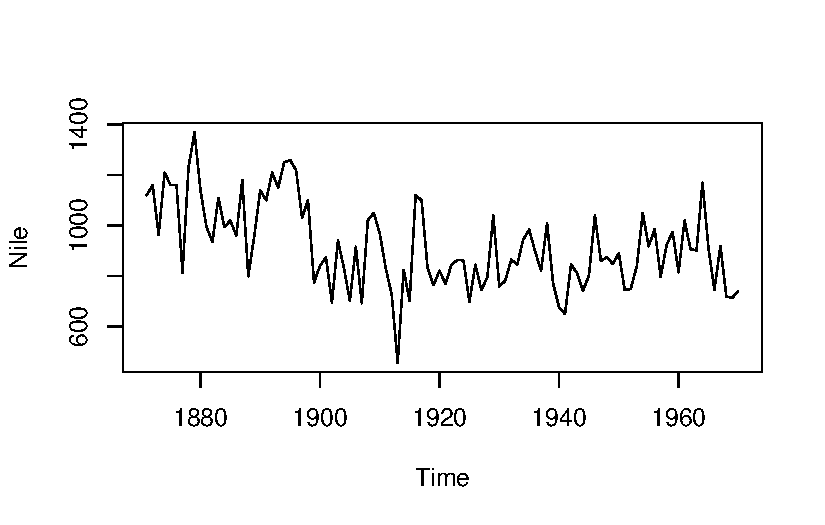
\includegraphics{./chapter14_files/figure-pdf/unnamed-chunk-4-1.pdf}

}

\end{figure}

\hypertarget{titanic}{%
\subsection{Titanic}\label{titanic}}

\textbf{Titanic}は、タイタニック号に乗船していた旅客とクルーの性別・船室(一等船室、二等船室、三等船室、クルー)・年齢区分(大人・子供)・生死に関する人数を4次元のArrayとしたものです。RではTitanicを用いることはそれほどありませんが、\href{https://www.kaggle.com/}{kaggle}という、機械学習の性能コンテストサイトでは機械学習の手習いとしてこのデータを用い、どのような性質の旅客であれば生存率が高いか、といった予測を行うモデルを作成するのによく用いられています。

\begin{Shaded}
\begin{Highlighting}[]
\NormalTok{Titanic}
\end{Highlighting}
\end{Shaded}

\begin{verbatim}
, , Age = Child, Survived = No

      Sex
Class  Male Female
  1st     0      0
  2nd     0      0
  3rd    35     17
  Crew    0      0

, , Age = Adult, Survived = No

      Sex
Class  Male Female
  1st   118      4
  2nd   154     13
  3rd   387     89
  Crew  670      3

, , Age = Child, Survived = Yes

      Sex
Class  Male Female
  1st     5      1
  2nd    11     13
  3rd    13     14
  Crew    0      0

, , Age = Adult, Survived = Yes

      Sex
Class  Male Female
  1st    57    140
  2nd    14     80
  3rd    75     76
  Crew  192     20
\end{verbatim}

\hypertarget{bostonhousing}{%
\subsection{BostonHousing}\label{bostonhousing}}

\textbf{BostonHousing}も、Rでというよりは機械学習の分野で、家賃の予測モデル作成の手習いとしてよく用いられています。BostonHousingは、その名の通りボストンの住宅価格と地域周辺の犯罪率・住宅の部屋数・税率・高速道路へのアクセスなどを、1970年のセンサス(国勢調査)から収集してまとめたものです。Rでは、mlbenchパッケージ(機械学習のベンチマークデータセットを集めたもの)に含まれており、使用するためにはmlbenchパッケージをインストール・ロードする必要があります。BostonHousingのデータ型はデータフレームです。

\begin{Shaded}
\begin{Highlighting}[]
\NormalTok{pacman}\SpecialCharTok{::}\FunctionTok{p\_load}\NormalTok{(mlbench)}
\FunctionTok{data}\NormalTok{(}\StringTok{"BostonHousing"}\NormalTok{)}
\FunctionTok{head}\NormalTok{(BostonHousing)}
\end{Highlighting}
\end{Shaded}

\begin{verbatim}
     crim zn indus chas   nox    rm  age    dis rad tax ptratio      b lstat
1 0.00632 18  2.31    0 0.538 6.575 65.2 4.0900   1 296    15.3 396.90  4.98
2 0.02731  0  7.07    0 0.469 6.421 78.9 4.9671   2 242    17.8 396.90  9.14
3 0.02729  0  7.07    0 0.469 7.185 61.1 4.9671   2 242    17.8 392.83  4.03
4 0.03237  0  2.18    0 0.458 6.998 45.8 6.0622   3 222    18.7 394.63  2.94
5 0.06905  0  2.18    0 0.458 7.147 54.2 6.0622   3 222    18.7 396.90  5.33
6 0.02985  0  2.18    0 0.458 6.430 58.7 6.0622   3 222    18.7 394.12  5.21
  medv
1 24.0
2 21.6
3 34.7
4 33.4
5 36.2
6 28.7
\end{verbatim}

\hypertarget{diamonds}{%
\subsection{diamonds}\label{diamonds}}

\textbf{diamonds}はグラフ作成ライブラリである、ggplot2に含まれるデータセットです。ggplot2を用いたグラフ作成例ではよく用いられています。diamondsはダイヤモンドのカラット数、透明性、カット、価格などをまとめたデータフレームです。

\begin{Shaded}
\begin{Highlighting}[]
\FunctionTok{head}\NormalTok{(ggplot2}\SpecialCharTok{::}\NormalTok{diamonds)}
\end{Highlighting}
\end{Shaded}

\begin{verbatim}
# A tibble: 6 x 10
  carat cut       color clarity depth table price     x     y     z
  <dbl> <ord>     <ord> <ord>   <dbl> <dbl> <int> <dbl> <dbl> <dbl>
1  0.23 Ideal     E     SI2      61.5    55   326  3.95  3.98  2.43
2  0.21 Premium   E     SI1      59.8    61   326  3.89  3.84  2.31
3  0.23 Good      E     VS1      56.9    65   327  4.05  4.07  2.31
4  0.29 Premium   I     VS2      62.4    58   334  4.2   4.23  2.63
5  0.31 Good      J     SI2      63.3    58   335  4.34  4.35  2.75
6  0.24 Very Good J     VVS2     62.8    57   336  3.94  3.96  2.48
\end{verbatim}

\hypertarget{gapminder}{%
\subsection{Gapminder}\label{gapminder}}

Gapminderは1952~2007年の各国のGDP、一人当たりGDP、寿命、人口をデータフレームとしてまとめたものです。このデータは、\href{https://www.gapminder.org/}{Gapminder
Foundation}(スウェーデンのNPO、所得格差の認知を推進する活動を行っている)が提供しているデータです。このデータも、Rでのグラフ作成の例でよく用いられているものです。Rでは、gapminderパッケージにデータセットが含まれています。

\begin{Shaded}
\begin{Highlighting}[]
\FunctionTok{head}\NormalTok{(gapminder}\SpecialCharTok{::}\NormalTok{gapminder)}
\end{Highlighting}
\end{Shaded}

\begin{verbatim}
# A tibble: 6 x 6
  country     continent  year lifeExp      pop gdpPercap
  <fct>       <fct>     <int>   <dbl>    <int>     <dbl>
1 Afghanistan Asia       1952    28.8  8425333      779.
2 Afghanistan Asia       1957    30.3  9240934      821.
3 Afghanistan Asia       1962    32.0 10267083      853.
4 Afghanistan Asia       1967    34.0 11537966      836.
5 Afghanistan Asia       1972    36.1 13079460      740.
6 Afghanistan Asia       1977    38.4 14880372      786.
\end{verbatim}

\bookmarksetup{startatroot}

\hypertarget{applyux95a2ux6570ux7fa4}{%
\chapter{apply関数群}\label{applyux95a2ux6570ux7fa4}}

Rを代表する便利な関数やライブラリは何か?、と聞かれると、2010年ごろまでは\textbf{apply関数群}を挙げるのが一般的でした。apply関数群を用いれば、他の言語では繰り返し計算で数行プログラムを書かないといけないような状況でも、たった1つの関数で高速に計算ができます。当時、Rでは繰り返し計算を使わず、apply関数群を使うのが標準的な方法でした。現在では、2010年以降に開発された\textbf{dplyr・tidyrパッケージ}を用いて計算を行うのが一般的となり、apply関数群は使われなくなってきていますが、ちょっとした機会に使うと便利な関数群です。

この章では、まず繰り返し計算によるベクター・データフレームの計算について解説し、次に繰り返しを用いず計算を行うapply関数群について説明していきます。

\hypertarget{ux7e70ux308aux8fd4ux3057ux8a08ux7b97}{%
\section{繰り返し計算}\label{ux7e70ux308aux8fd4ux3057ux8a08ux7b97}}

ベクターのような,多数の要素を含むオブジェクトを用いて演算を行う場合,R以外の言語では通常\textbf{繰り返し計算}を用います.繰り返し計算は5章で説明した通り,for文やwhile文,repeat文などです.プログラミング言語によって繰り返し計算の形は異なりますが,たくさんの要素を持つオブジェクトの演算では,繰り返し計算は有効な計算方法の一つです.

\hypertarget{ux7e70ux308aux8fd4ux3057ux8a08ux7b97ux3068ux30d9ux30afux30bfux30fc}{%
\section{繰り返し計算とベクター}\label{ux7e70ux308aux8fd4ux3057ux8a08ux7b97ux3068ux30d9ux30afux30bfux30fc}}

では,Rでの繰り返し計算を見てみましょう.下の例では,ベクターの要素に演算を行い,結果をベクターで返す繰り返し計算を行っています.

Rでfor文を用いてベクターの要素に演算を行う場合には,

\begin{itemize}
\tightlist
\item
  NULLを代入しただけの空っぽの変数を作る
\item
  繰り返し回数を演算に用いるベクターの長さで指定する
\item
  ベクターの要素をインデックスで取り出し,演算する
\item
  空っぽの変数に,c関数で演算結果を付け足す
\end{itemize}

といった計算を行うことがあります.

下の例では,変数vは1~10の連続する長さ10の整数ベクター,v\_newはNULL(空)のオブジェクトです.

for文では,iに1:length(v)の要素が繰り返し計算ごとに代入されます.つまり1回目の繰り返し計算ではiは1,2回目ではiは2\ldots となり,iにlength(v),つまり10が代入された計算が終わると,繰り返し計算が終了します.

さらに,for文中では,v{[}i{]},つまりiをインデックスにしてvの要素を取り出しています.1回目の繰り返し計算ではiが1ですので,v{[}i{]}はvの1つ目の要素,2回目の繰り返し計算ではv{[}i{]}はvの2つ目の要素となります.v{[}i{]}を3倍して5を足した結果を一時的にtempという変数に代入しています.

for文の中では,\textbf{「v\_new \textless- c(v\_new,
temp)」}という形で,空の変数であるv\_newに,計算結果をc関数で繋いだものを,v\_newに代入する,という変な演算を行っています.この演算では,1週目ではc(NULL,
temp)をv\_newに代入することで,v\_newはtempを1つだけ持つベクターに変化しています.2週目以降は,v\_newのベクターの要素の後に新しく計算したtempが付け加えられます.これを繰り返すことで,v\_newにはtempの計算結果がベクターとして記録されていきます.

最終的に,v\_newはvの各要素を3倍して5を足したベクターとして演算が終了します.

\begin{Shaded}
\begin{Highlighting}[]
\NormalTok{v }\OtherTok{\textless{}{-}} \DecValTok{1}\SpecialCharTok{:}\DecValTok{10} \CommentTok{\# vは1\textasciitilde{}10の整数ベクター}

\NormalTok{v\_new }\OtherTok{\textless{}{-}} \ConstantTok{NULL} \CommentTok{\# 計算結果を代入するNULLが入った変数}

\ControlFlowTok{for}\NormalTok{(i }\ControlFlowTok{in} \DecValTok{1}\SpecialCharTok{:}\FunctionTok{length}\NormalTok{(v))\{ }\CommentTok{\# vの長さ分計算する}
\NormalTok{  temp }\OtherTok{\textless{}{-}}\NormalTok{ v[i] }\SpecialCharTok{*} \DecValTok{3} \SpecialCharTok{+} \DecValTok{5}
\NormalTok{  v\_new }\OtherTok{\textless{}{-}} \FunctionTok{c}\NormalTok{(v\_new, temp) }\CommentTok{\# v\_newにv[i]を演算した結果をつなげる}
\NormalTok{\}}

\NormalTok{v\_new }\CommentTok{\# 演算結果}
\end{Highlighting}
\end{Shaded}

\begin{verbatim}
 [1]  8 11 14 17 20 23 26 29 32 35
\end{verbatim}

上記のようなfor文の演算は,Rでは非常によろしくない,典型的なバッドノウハウであるとされています.そもそもRでのベクターの演算に繰り返し文を使う必要がないので,上記のfor文は下のように書き換えることができます.\textbf{ベクターの演算の方が,for文を用いた演算よりずっと速い}ため,Rでベクターの要素を演算に用いる場合には,繰り返し計算ではなく,ベクターの演算を用いることが推奨されています.

\begin{Shaded}
\begin{Highlighting}[]
\NormalTok{v }\SpecialCharTok{*} \DecValTok{3} \SpecialCharTok{+} \DecValTok{5}
\end{Highlighting}
\end{Shaded}

\begin{verbatim}
 [1]  8 11 14 17 20 23 26 29 32 35
\end{verbatim}

上のfor文にはもう一点問題があります.v\_newというベクターに対して,数値を付け足すという演算を繰り返しています.このような場合,v\_newの長さが伸びていくため,Rの内部では,\textbf{要素が付け加えられる度にv\_newというベクターを新しく作り直し,古いものは削除する}という演算が行われることになります.この\textbf{「作り直し」て「削除する」}という演算に時間がかかるため,上記のような書き方では演算速度に問題が生じます.

このような「作り直し」て「削除する」プロセスを省くためには,インデックスに代入する方法を用います.あらかじめ結果と同じ長さのベクターを準備しておき,このベクターの要素に演算結果を代入します.このような形にすると,v\_new自体を作り直すプロセスがなくなり,演算速度が速くなるとされています.

この,結果と同じ長さのベクターを準備するときには,\textbf{numeric関数}を用います.numeric関数は数値を1つ引数に取り,数値に応じた長さの,要素が0だけのベクターを作成する関数です.このnumeric関数を用いて演算結果と同じ長さのベクターを作成しておくことで,そのインデックスに演算結果を代入していくことができます.

\begin{Shaded}
\begin{Highlighting}[]
\FunctionTok{numeric}\NormalTok{(}\DecValTok{5}\NormalTok{) }\CommentTok{\# 0が5つ入ったベクター}
\end{Highlighting}
\end{Shaded}

\begin{verbatim}
[1] 0 0 0 0 0
\end{verbatim}

\begin{Shaded}
\begin{Highlighting}[]
\NormalTok{v\_new }\OtherTok{\textless{}{-}} \FunctionTok{numeric}\NormalTok{(}\FunctionTok{length}\NormalTok{(v)) }\CommentTok{\# v\_newは0がvと同じ長さだけ並んだベクター}

\ControlFlowTok{for}\NormalTok{(i }\ControlFlowTok{in} \DecValTok{1}\SpecialCharTok{:}\FunctionTok{length}\NormalTok{(v))\{ }\CommentTok{\# vの長さ分計算する}
\NormalTok{  v\_new[i] }\OtherTok{\textless{}{-}}\NormalTok{ v[i] }\SpecialCharTok{*} \DecValTok{3} \SpecialCharTok{+} \DecValTok{5} \CommentTok{\# v\_new[i]にv[i]を演算した結果を代入}
\NormalTok{\}}

\NormalTok{v\_new }\CommentTok{\# 演算結果}
\end{Highlighting}
\end{Shaded}

\begin{verbatim}
 [1]  8 11 14 17 20 23 26 29 32 35
\end{verbatim}

\hypertarget{ux7e70ux308aux8fd4ux3057ux8a08ux7b97ux3068ux30c7ux30fcux30bfux30d5ux30ecux30fcux30e0}{%
\section{繰り返し計算とデータフレーム}\label{ux7e70ux308aux8fd4ux3057ux8a08ux7b97ux3068ux30c7ux30fcux30bfux30d5ux30ecux30fcux30e0}}

データフレームの要素に対して繰り返し計算をする場合にも、上のベクターでの繰り返し計算と同様の手法が使えます。下の計算では、iris\_editedという変数にNULLを代入し、この空のiris\_editedにベクターをrbind関数で結合したものをiris\_editedに代入するという計算をしています。rbind関数は行を追加する関数ですので、計算結果を含むベクターはiris\_editedの一番下の行に追加されます。

このような繰り返し計算を行うと、iris\_editedは自動的にNULLから\textbf{行列}に変換されます。また、計算途中でiris\$Species(因子)を文字列に変換し、文字列と数値の計算結果をベクターにまとめているため、数値計算結果は自動的に文字列に変換されています。その結果、繰り返し計算後に得られるiris\_editedは\textbf{文字列の行列}になっています。

行列は、as.data.frame関数でデータフレームに変換できます。ただし、文字列の行列の要素は文字列型のまま変換されるため、結果が数値に見えても文字列になっている場合があります.

このように、データフレームを直接繰り返し計算に用いると、データ型の変換が頻繁に起こり、計算結果を予測するのが難しくなります。繰り返し計算時には、取り扱っている変数の型がどのように変化しているのか、常に注意が必要です。

\begin{Shaded}
\begin{Highlighting}[]
\FunctionTok{head}\NormalTok{(iris)}
\end{Highlighting}
\end{Shaded}

\begin{verbatim}
  Sepal.Length Sepal.Width Petal.Length Petal.Width Species
1          5.1         3.5          1.4         0.2  setosa
2          4.9         3.0          1.4         0.2  setosa
3          4.7         3.2          1.3         0.2  setosa
4          4.6         3.1          1.5         0.2  setosa
5          5.0         3.6          1.4         0.2  setosa
6          5.4         3.9          1.7         0.4  setosa
\end{verbatim}

\begin{Shaded}
\begin{Highlighting}[]
\NormalTok{iris\_edited }\OtherTok{\textless{}{-}} \ConstantTok{NULL}

\ControlFlowTok{for}\NormalTok{(i }\ControlFlowTok{in} \DecValTok{1}\SpecialCharTok{:}\FunctionTok{nrow}\NormalTok{(iris))\{}
  \CommentTok{\# iris$Speciesは因子で、そのままだと数値に変換されるため、文字列に変換しておく}
\NormalTok{  species }\OtherTok{\textless{}{-}} \FunctionTok{as.character}\NormalTok{(iris}\SpecialCharTok{$}\NormalTok{Species[i]) }
  
  \CommentTok{\# Sepal.LengthとSepal.Widthの積を計算}
\NormalTok{  Sepal\_multiple }\OtherTok{\textless{}{-}}\NormalTok{ iris}\SpecialCharTok{$}\NormalTok{Sepal.Length[i] }\SpecialCharTok{*}\NormalTok{ iris}\SpecialCharTok{$}\NormalTok{Sepal.Width[i]}
  
  \CommentTok{\# species(文字列)と計算結果をベクターにまとめる(文字列のベクターに変換)}
\NormalTok{  temp\_vec }\OtherTok{\textless{}{-}} \FunctionTok{c}\NormalTok{(species, Sepal\_multiple)}
  
  \CommentTok{\# ベクターをiris\_editedの行として追加(iris\_editedは行列になる)}
\NormalTok{  iris\_edited }\OtherTok{\textless{}{-}} \FunctionTok{rbind}\NormalTok{(iris\_edited, temp\_vec)}
\NormalTok{\}}

\FunctionTok{dim}\NormalTok{(iris\_edited) }\CommentTok{\# iris\_editedは150行2列}
\end{Highlighting}
\end{Shaded}

\begin{verbatim}
[1] 150   2
\end{verbatim}

\begin{Shaded}
\begin{Highlighting}[]
\FunctionTok{class}\NormalTok{(iris\_edited) }\CommentTok{\# iris\_editedは行列(matrix)}
\end{Highlighting}
\end{Shaded}

\begin{verbatim}
[1] "matrix" "array" 
\end{verbatim}

\begin{Shaded}
\begin{Highlighting}[]
\FunctionTok{head}\NormalTok{(iris\_edited) }\CommentTok{\# 文字列の行列になっている}
\end{Highlighting}
\end{Shaded}

\begin{verbatim}
         [,1]     [,2]   
temp_vec "setosa" "17.85"
temp_vec "setosa" "14.7" 
temp_vec "setosa" "15.04"
temp_vec "setosa" "14.26"
temp_vec "setosa" "18"   
temp_vec "setosa" "21.06"
\end{verbatim}

ベクターの繰り返し計算で述べたように、変数に要素を追加して,サイズが変化すると、変数を「作り直し」て「削除する」プロセスが繰り返され、計算のコストが大きくなります。計算のコストが大きくなると演算に時間がかかるため、このようなNULLに要素を追加するのは避けた方がよいとされています。ですので、上のような計算では、あらかじめ結果と同じサイズの行列を準備し、その行列の要素に計算結果を追加していくのが良いとされています。

\begin{Shaded}
\begin{Highlighting}[]
\FunctionTok{head}\NormalTok{(iris)}
\end{Highlighting}
\end{Shaded}

\begin{verbatim}
  Sepal.Length Sepal.Width Petal.Length Petal.Width Species
1          5.1         3.5          1.4         0.2  setosa
2          4.9         3.0          1.4         0.2  setosa
3          4.7         3.2          1.3         0.2  setosa
4          4.6         3.1          1.5         0.2  setosa
5          5.0         3.6          1.4         0.2  setosa
6          5.4         3.9          1.7         0.4  setosa
\end{verbatim}

\begin{Shaded}
\begin{Highlighting}[]
\NormalTok{iris\_edited }\OtherTok{\textless{}{-}} \FunctionTok{matrix}\NormalTok{(}\DecValTok{0}\NormalTok{, }\AttributeTok{nrow=}\DecValTok{150}\NormalTok{, }\AttributeTok{ncol=}\DecValTok{2}\NormalTok{)}

\ControlFlowTok{for}\NormalTok{(i }\ControlFlowTok{in} \DecValTok{1}\SpecialCharTok{:}\FunctionTok{nrow}\NormalTok{(iris))\{}
\NormalTok{  species }\OtherTok{\textless{}{-}} \FunctionTok{as.character}\NormalTok{(iris}\SpecialCharTok{$}\NormalTok{Species[i])}
\NormalTok{  Sepal\_multiple }\OtherTok{\textless{}{-}}\NormalTok{ iris}\SpecialCharTok{$}\NormalTok{Sepal.Length[i] }\SpecialCharTok{*}\NormalTok{ iris}\SpecialCharTok{$}\NormalTok{Sepal.Width[i]}
\NormalTok{  temp\_vec }\OtherTok{\textless{}{-}} \FunctionTok{c}\NormalTok{(species, Sepal\_multiple)}
\NormalTok{  iris\_edited[i, ] }\OtherTok{\textless{}{-}}\NormalTok{ temp\_vec}
\NormalTok{\}}

\FunctionTok{dim}\NormalTok{(iris\_edited) }\CommentTok{\# iris\_editedは150行2列}
\end{Highlighting}
\end{Shaded}

\begin{verbatim}
[1] 150   2
\end{verbatim}

\begin{Shaded}
\begin{Highlighting}[]
\FunctionTok{class}\NormalTok{(iris\_edited) }\CommentTok{\# iris\_editedは行列(matrix)}
\end{Highlighting}
\end{Shaded}

\begin{verbatim}
[1] "matrix" "array" 
\end{verbatim}

\begin{Shaded}
\begin{Highlighting}[]
\FunctionTok{head}\NormalTok{(iris\_edited) }\CommentTok{\# 文字列の行列になっている}
\end{Highlighting}
\end{Shaded}

\begin{verbatim}
     [,1]     [,2]   
[1,] "setosa" "17.85"
[2,] "setosa" "14.7" 
[3,] "setosa" "15.04"
[4,] "setosa" "14.26"
[5,] "setosa" "18"   
[6,] "setosa" "21.06"
\end{verbatim}

上記のように、Rでは繰り返し計算で変数の「作り直し」が起きたり、データ型がころころ変わったりするため、繰り返し計算でベクターやデータフレームの要素を取り扱うのは推奨されていません。ただし、繰り返し計算は演算の過程が捉えやすく、後から読んで理解しやすい構造をしています.NULLオブジェクトにデータを追加していくと、結果として得られるオブジェクトのサイズがわかっていなくても演算できるという利点があります。

2000年頃のPCは性能が低く、計算コストに気を払う必要がありましたが、現在では繰り返し計算を回しても大して時間がかからなくなりました。よほど大きいデータフレーム(数万~数十万行)を取り扱う場合を除けば、繰り返し計算が問題となることは少なくなったと感じます。データの取り扱いが一度きり(ad
hoc)の場合には以下のapplyを使っても、繰り返し計算を使っても大差ないため、好みの、わかりやすい方法を用いればよいでしょう。

\hypertarget{applyux95a2ux6570ux7fa4-1}{%
\section{apply関数群}\label{applyux95a2ux6570ux7fa4-1}}

Rでのデータフレーム演算の「お作法」では、繰り返し計算ではなく、apply関数群を用いることとされています。apply関数群にはapply,
mapply, lapply, sapply, tapply, aggregate,
byなど、かなりたくさんの関数があり、それぞれ少し癖のある使い方が求められます。以下の表1にapply関数群についてまとめます。

\begin{longtable}[]{@{}l@{}}
\caption{表1
apply関数群(funは関数,factは因子,marginは方向を指す)}\tabularnewline
\toprule()
x \\
\midrule()
\endfirsthead
\toprule()
x \\
\midrule()
\endhead
apply(x, margin, fun) \\
mapply(fun, 引数1, 引数2\ldots) \\
lapply(list, fun) \\
sapply(list, fun) \\
vapply(x, fun, fun.value) \\
replicate(n, calc) \\
tapply(x, fact, fun) \\
sweep(x, margin, y) \\
aggregate(x, by, fun) \\
aggregate(formula, data) \\
by(x, by, fun) \\
\bottomrule()
\end{longtable}

\hypertarget{applyux95a2ux6570}{%
\subsection{apply関数}\label{applyux95a2ux6570}}

apply関数群の中で最も基本的なものが、\textbf{apply関数}です。apply関数は第一引数にデータフレーム(もしくは行列)を取り、第二引数にMARGIN、第三引数に関数を取ります。第二引数のMARGINは1か2を取り、1を取ると行(横)方向、2を取ると列(縦)方向のベクターを計算対象とします。apply関数はデータフレームの要素に、MARGINで指定した方向に、第三引数で指定した関数を適用します。第三引数に指定する関数には,Rに備わっている関数,自作した関数の両方を用いることができます.

apply関数の演算では、(特に行方向、MARGIN =
1の時には)データ型が一致していることが必要となります。apply関数の使い方を以下の図1に示します。

\begin{figure}

{\centering 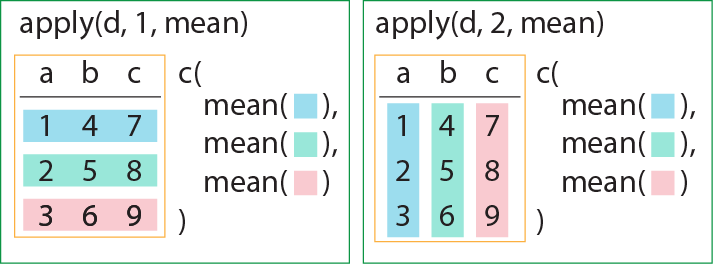
\includegraphics{././image/chapter15_apply.png}

}

\caption{図1:apply関数の使い方}

\end{figure}

\begin{Shaded}
\begin{Highlighting}[]
\FunctionTok{apply}\NormalTok{(iris[, }\DecValTok{1}\SpecialCharTok{:}\DecValTok{4}\NormalTok{], }\DecValTok{1}\NormalTok{, sum) }\CommentTok{\# 行方向に和を求める}
\end{Highlighting}
\end{Shaded}

\begin{verbatim}
  [1] 10.2  9.5  9.4  9.4 10.2 11.4  9.7 10.1  8.9  9.6 10.8 10.0  9.3  8.5 11.2
 [16] 12.0 11.0 10.3 11.5 10.7 10.7 10.7  9.4 10.6 10.3  9.8 10.4 10.4 10.2  9.7
 [31]  9.7 10.7 10.9 11.3  9.7  9.6 10.5 10.0  8.9 10.2 10.1  8.4  9.1 10.7 11.2
 [46]  9.5 10.7  9.4 10.7  9.9 16.3 15.6 16.4 13.1 15.4 14.3 15.9 11.6 15.4 13.2
 [61] 11.5 14.6 13.2 15.1 13.4 15.6 14.6 13.6 14.4 13.1 15.7 14.2 15.2 14.8 14.9
 [76] 15.4 15.8 16.4 14.9 12.8 12.8 12.6 13.6 15.4 14.4 15.5 16.0 14.3 14.0 13.3
 [91] 13.7 15.1 13.6 11.6 13.8 14.1 14.1 14.7 11.7 13.9 18.1 15.5 18.1 16.6 17.5
[106] 19.3 13.6 18.3 16.8 19.4 16.8 16.3 17.4 15.2 16.1 17.2 16.8 20.4 19.5 14.7
[121] 18.1 15.3 19.2 15.7 17.8 18.2 15.6 15.8 16.9 17.6 18.2 20.1 17.0 15.7 15.7
[136] 19.1 17.7 16.8 15.6 17.5 17.8 17.4 15.5 18.2 18.2 17.2 15.7 16.7 17.3 15.8
\end{verbatim}

\begin{Shaded}
\begin{Highlighting}[]
\FunctionTok{apply}\NormalTok{(iris[, }\DecValTok{1}\SpecialCharTok{:}\DecValTok{4}\NormalTok{], }\DecValTok{2}\NormalTok{, sum) }\CommentTok{\# 列方向に和を求める}
\end{Highlighting}
\end{Shaded}

\begin{verbatim}
Sepal.Length  Sepal.Width Petal.Length  Petal.Width 
       876.5        458.6        563.7        179.9 
\end{verbatim}

\begin{Shaded}
\begin{Highlighting}[]
\CommentTok{\# 自作の関数}
\NormalTok{func1 }\OtherTok{\textless{}{-}} \ControlFlowTok{function}\NormalTok{(x)\{}\FunctionTok{sum}\NormalTok{(}\FunctionTok{sqrt}\NormalTok{(x) }\SpecialCharTok{*} \FunctionTok{log}\NormalTok{(x))\}}

\FunctionTok{apply}\NormalTok{(iris[, }\DecValTok{1}\SpecialCharTok{:}\DecValTok{4}\NormalTok{], }\DecValTok{2}\NormalTok{, func1)}
\end{Highlighting}
\end{Shaded}

\begin{verbatim}
Sepal.Length  Sepal.Width Petal.Length  Petal.Width 
   638.50578    292.37383    373.96812     32.26917 
\end{verbatim}

\begin{Shaded}
\begin{Highlighting}[]
\CommentTok{\# apply(iris[, 1:4], 2, \textbackslash{}(x)\{x + 1\}) \# 無名関数も利用できる}
\end{Highlighting}
\end{Shaded}

\hypertarget{ux6b21ux5143ux4ee5ux4e0aux306earrayux306bapplyux3092ux9069ux7528ux3059ux308b}{%
\subsubsection{3次元以上のarrayにapplyを適用する}\label{ux6b21ux5143ux4ee5ux4e0aux306earrayux306bapplyux3092ux9069ux7528ux3059ux308b}}

apply関数は3次元以上のarrayを引数に取ることもできます。3次元以上のarrayを引数に取る場合には、MARGINの設定がやや複雑になります。MARGINに1つの値を入れた場合には、その次元を残す形で関数を適用します。MARGINに2つの値を入れた場合には、その2つの次元を残して関数を適用します。MARGINに2つ以上の値を指定する際には、ベクターを用います。

\begin{Shaded}
\begin{Highlighting}[]
\NormalTok{UCBAdmissions }\CommentTok{\# 3次元アレイ}
\end{Highlighting}
\end{Shaded}

\begin{verbatim}
, , Dept = A

          Gender
Admit      Male Female
  Admitted  512     89
  Rejected  313     19

, , Dept = B

          Gender
Admit      Male Female
  Admitted  353     17
  Rejected  207      8

, , Dept = C

          Gender
Admit      Male Female
  Admitted  120    202
  Rejected  205    391

, , Dept = D

          Gender
Admit      Male Female
  Admitted  138    131
  Rejected  279    244

, , Dept = E

          Gender
Admit      Male Female
  Admitted   53     94
  Rejected  138    299

, , Dept = F

          Gender
Admit      Male Female
  Admitted   22     24
  Rejected  351    317
\end{verbatim}

\begin{Shaded}
\begin{Highlighting}[]
\FunctionTok{dimnames}\NormalTok{(UCBAdmissions) }\CommentTok{\# 次元の順番はAdmit, Gender, Deptの順}
\end{Highlighting}
\end{Shaded}

\begin{verbatim}
$Admit
[1] "Admitted" "Rejected"

$Gender
[1] "Male"   "Female"

$Dept
[1] "A" "B" "C" "D" "E" "F"
\end{verbatim}

\begin{Shaded}
\begin{Highlighting}[]
\FunctionTok{apply}\NormalTok{(UCBAdmissions, }\DecValTok{1}\NormalTok{, mean) }\CommentTok{\# 1次元目(Admit)の平均を求める}
\end{Highlighting}
\end{Shaded}

\begin{verbatim}
Admitted Rejected 
146.2500 230.9167 
\end{verbatim}

\begin{Shaded}
\begin{Highlighting}[]
\FunctionTok{apply}\NormalTok{(UCBAdmissions, }\DecValTok{2}\NormalTok{, mean) }\CommentTok{\# 2次元目(Gender)の平均を求める}
\end{Highlighting}
\end{Shaded}

\begin{verbatim}
    Male   Female 
224.2500 152.9167 
\end{verbatim}

\begin{Shaded}
\begin{Highlighting}[]
\FunctionTok{apply}\NormalTok{(UCBAdmissions, }\DecValTok{3}\NormalTok{, mean) }\CommentTok{\# 3次元目(Dept)の平均を求める}
\end{Highlighting}
\end{Shaded}

\begin{verbatim}
     A      B      C      D      E      F 
233.25 146.25 229.50 198.00 146.00 178.50 
\end{verbatim}

\begin{Shaded}
\begin{Highlighting}[]
\FunctionTok{apply}\NormalTok{(UCBAdmissions, }\DecValTok{1}\SpecialCharTok{:}\DecValTok{2}\NormalTok{, mean) }\CommentTok{\# 3次元目(Dept)方向に平均を求める}
\end{Highlighting}
\end{Shaded}

\begin{verbatim}
          Gender
Admit          Male    Female
  Admitted 199.6667  92.83333
  Rejected 248.8333 213.00000
\end{verbatim}

\begin{Shaded}
\begin{Highlighting}[]
\FunctionTok{apply}\NormalTok{(UCBAdmissions, }\FunctionTok{c}\NormalTok{(}\DecValTok{1}\NormalTok{, }\DecValTok{3}\NormalTok{), mean) }\CommentTok{\# 2次元目(Gender)方向に平均を求める}
\end{Highlighting}
\end{Shaded}

\begin{verbatim}
          Dept
Admit          A     B   C     D     E   F
  Admitted 300.5 185.0 161 134.5  73.5  23
  Rejected 166.0 107.5 298 261.5 218.5 334
\end{verbatim}

\begin{Shaded}
\begin{Highlighting}[]
\FunctionTok{apply}\NormalTok{(UCBAdmissions, }\DecValTok{2}\SpecialCharTok{:}\DecValTok{3}\NormalTok{, mean) }\CommentTok{\# 1次元目(Admit)方向に平均を求める}
\end{Highlighting}
\end{Shaded}

\begin{verbatim}
        Dept
Gender       A     B     C     D     E     F
  Male   412.5 280.0 162.5 208.5  95.5 186.5
  Female  54.0  12.5 296.5 187.5 196.5 170.5
\end{verbatim}

\hypertarget{mapplyux95a2ux6570}{%
\subsection{mapply関数}\label{mapplyux95a2ux6570}}

\textbf{mapply関数}は、関数が2種類以上の引数を取る場合に用います。mapply関数はapply関数とは引数の順番が異なり、適用する関数が第一引数になります。続いて適用する関数の引数をベクターで取ります。mapply関数の返り値は適用する関数により異なり、関数の返り値が1つならmapply関数の返り値はベクター、返り値が2つ以上ならmapply関数の返り値はリストになります。

\begin{figure}

{\centering 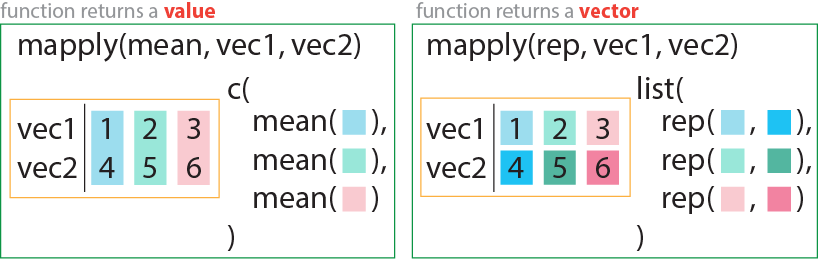
\includegraphics{././image/chapter15_mapply.png}

}

\caption{図2:mapply関数の使い方}

\end{figure}

\begin{Shaded}
\begin{Highlighting}[]
\FunctionTok{mapply}\NormalTok{(mean, }\DecValTok{1}\SpecialCharTok{:}\DecValTok{4}\NormalTok{, }\DecValTok{2}\SpecialCharTok{:}\DecValTok{5}\NormalTok{)}
\end{Highlighting}
\end{Shaded}

\begin{verbatim}
[1] 1 2 3 4
\end{verbatim}

\begin{Shaded}
\begin{Highlighting}[]
\NormalTok{lst }\OtherTok{\textless{}{-}} \FunctionTok{mapply}\NormalTok{(rep, }\AttributeTok{times =} \DecValTok{1}\SpecialCharTok{:}\DecValTok{4}\NormalTok{, }\AttributeTok{x =} \DecValTok{4}\SpecialCharTok{:}\DecValTok{1}\NormalTok{) }\CommentTok{\# 関数の引数を指定して、ベクターで与える 複数の引数を取れる}
\NormalTok{lst}
\end{Highlighting}
\end{Shaded}

\begin{verbatim}
[[1]]
[1] 4

[[2]]
[1] 3 3

[[3]]
[1] 2 2 2

[[4]]
[1] 1 1 1 1
\end{verbatim}

\begin{Shaded}
\begin{Highlighting}[]
\CommentTok{\# 無名関数も使える}
\FunctionTok{mapply}\NormalTok{(\textbackslash{}(x, y)\{x }\SpecialCharTok{/}\NormalTok{ y\}, }\AttributeTok{x =} \DecValTok{1}\SpecialCharTok{:}\DecValTok{5}\NormalTok{, }\AttributeTok{y =} \DecValTok{5}\SpecialCharTok{:}\DecValTok{1}\NormalTok{)}
\end{Highlighting}
\end{Shaded}

\begin{verbatim}
[1] 0.2 0.5 1.0 2.0 5.0
\end{verbatim}

\hypertarget{lapplyux95a2ux6570sapplyux95a2ux6570}{%
\subsection{lapply関数/sapply関数}\label{lapplyux95a2ux6570sapplyux95a2ux6570}}

\textbf{lapply関数}はリストを引数に取る関数です。lapply関数は第一引数にリスト、第二引数に関数を取り、リストの各要素に関数を適用します。lapply関数は返り値にリストを取ります。データフレームはリストですので、lapply関数はapply(x,
2, FUN)、つまり列方向に関数を適用するのと同じ計算を行うことができます。

\textbf{sapply関数}は返り値がベクターになったlapply関数です。関数の返り値が2つの値であれば、sapply関数は行列を返します。

\begin{figure}

{\centering 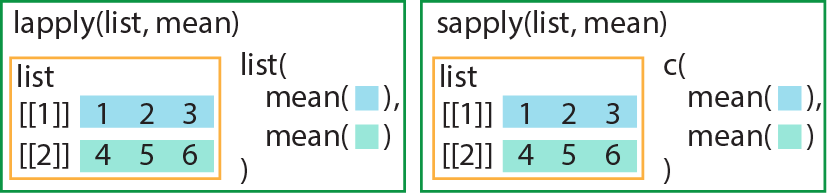
\includegraphics{././image/chapter15_lapply.png}

}

\caption{図3:lapply/sapply関数の使い方}

\end{figure}

\begin{Shaded}
\begin{Highlighting}[]
\FunctionTok{lapply}\NormalTok{(lst, sum) }\CommentTok{\# リストの各要素に関数を適用する(返り値はリスト)}
\end{Highlighting}
\end{Shaded}

\begin{verbatim}
[[1]]
[1] 4

[[2]]
[1] 6

[[3]]
[1] 6

[[4]]
[1] 4
\end{verbatim}

\begin{Shaded}
\begin{Highlighting}[]
\FunctionTok{lapply}\NormalTok{(iris[, }\DecValTok{1}\SpecialCharTok{:}\DecValTok{4}\NormalTok{], sum) }\CommentTok{\# データフレームは列方向のリストなので、適用可能}
\end{Highlighting}
\end{Shaded}

\begin{verbatim}
$Sepal.Length
[1] 876.5

$Sepal.Width
[1] 458.6

$Petal.Length
[1] 563.7

$Petal.Width
[1] 179.9
\end{verbatim}

\begin{Shaded}
\begin{Highlighting}[]
\FunctionTok{lapply}\NormalTok{(lst, summary)}
\end{Highlighting}
\end{Shaded}

\begin{verbatim}
[[1]]
   Min. 1st Qu.  Median    Mean 3rd Qu.    Max. 
      4       4       4       4       4       4 

[[2]]
   Min. 1st Qu.  Median    Mean 3rd Qu.    Max. 
      3       3       3       3       3       3 

[[3]]
   Min. 1st Qu.  Median    Mean 3rd Qu.    Max. 
      2       2       2       2       2       2 

[[4]]
   Min. 1st Qu.  Median    Mean 3rd Qu.    Max. 
      1       1       1       1       1       1 
\end{verbatim}

\begin{Shaded}
\begin{Highlighting}[]
\FunctionTok{sapply}\NormalTok{(lst, sum) }\CommentTok{\# 返り値がベクターのlapply}
\end{Highlighting}
\end{Shaded}

\begin{verbatim}
[1] 4 6 6 4
\end{verbatim}

\begin{Shaded}
\begin{Highlighting}[]
\FunctionTok{sapply}\NormalTok{(iris[, }\DecValTok{1}\SpecialCharTok{:}\DecValTok{4}\NormalTok{], sum)}
\end{Highlighting}
\end{Shaded}

\begin{verbatim}
Sepal.Length  Sepal.Width Petal.Length  Petal.Width 
       876.5        458.6        563.7        179.9 
\end{verbatim}

\hypertarget{vapplyux95a2ux6570}{%
\subsection{vapply関数}\label{vapplyux95a2ux6570}}

\textbf{vapply関数}は関数が複数の返り値を持つときに用いる関数です。vapply関数の第一引数はベクターやリスト、第二引数は複数の返り値を取る関数です。vapply関数はこの返り値を行列に変換するのですが、この変換時の行名をFUN.VALUEという第三引数で設定します。FUN.VALUEの設定は名前付きベクターで、値は0とします。かなり癖が強いので、使われているところをほとんど見たことがない関数です。

\begin{figure}

{\centering 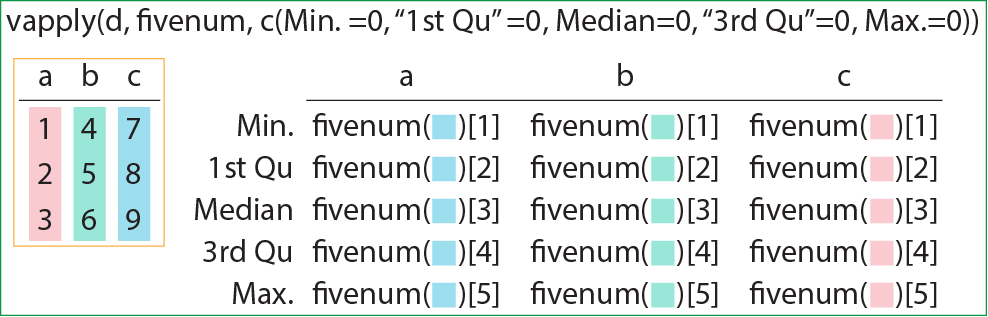
\includegraphics{././image/chapter15_vapply.png}

}

\caption{図3:vapply関数の使い方}

\end{figure}

\begin{Shaded}
\begin{Highlighting}[]
\FunctionTok{fivenum}\NormalTok{(}\DecValTok{1}\SpecialCharTok{:}\DecValTok{10}\NormalTok{) }\CommentTok{\# データを5つに集約する関数(最小値、第一四分位、中央値、第三四分位、最大値)}
\end{Highlighting}
\end{Shaded}

\begin{verbatim}
[1]  1.0  3.0  5.5  8.0 10.0
\end{verbatim}

\begin{Shaded}
\begin{Highlighting}[]
\FunctionTok{vapply}\NormalTok{(iris[, }\DecValTok{1}\SpecialCharTok{:}\DecValTok{4}\NormalTok{], fivenum, }\FunctionTok{c}\NormalTok{(}\AttributeTok{Min. =} \DecValTok{0}\NormalTok{, }\StringTok{"1st Qu"} \OtherTok{=} \DecValTok{0}\NormalTok{, }\AttributeTok{Median =} \DecValTok{0}\NormalTok{, }\StringTok{"3rd Qu"} \OtherTok{=} \DecValTok{0}\NormalTok{, }\AttributeTok{Max. =} \DecValTok{0}\NormalTok{)) }\CommentTok{\# 集約値をそれぞれ表示}
\end{Highlighting}
\end{Shaded}

\begin{verbatim}
       Sepal.Length Sepal.Width Petal.Length Petal.Width
Min.            4.3         2.0         1.00         0.1
1st Qu          5.1         2.8         1.60         0.3
Median          5.8         3.0         4.35         1.3
3rd Qu          6.4         3.3         5.10         1.8
Max.            7.9         4.4         6.90         2.5
\end{verbatim}

\hypertarget{replicateux95a2ux6570}{%
\subsection{replicate関数}\label{replicateux95a2ux6570}}

\textbf{replicate関数}は、第一引数に繰り返し計算の回数、第二引数に関数を取ります。replicate関数は関数の計算を繰り返し計算の回数だけ繰り返し、結果をベクターで返します。引数内の関数の引数を変えることはできないので、一見あまり意味がなさそうに見えます。しかし、Rでは乱数(ランダムな数値)を用いた計算を行うことが多く、乱数計算を繰り返すと同じ関数の返り値でも変化することがあります。したがって、replicate関数は乱数を使った計算で利用すると生きる関数となっています。

\begin{figure}

{\centering 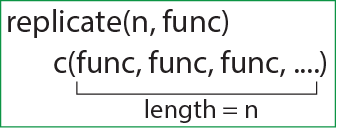
\includegraphics{././image/chapter15_replicate.png}

}

\caption{図5:replicate関数の使い方}

\end{figure}

\begin{Shaded}
\begin{Highlighting}[]
\FunctionTok{sample}\NormalTok{(}\DecValTok{1}\SpecialCharTok{:}\DecValTok{6}\NormalTok{, }\DecValTok{10}\NormalTok{, }\AttributeTok{replace=}\NormalTok{T) }\CommentTok{\# サイコロを10回ふる}
\end{Highlighting}
\end{Shaded}

\begin{verbatim}
 [1] 6 1 4 1 2 5 3 6 2 3
\end{verbatim}

\begin{Shaded}
\begin{Highlighting}[]
\FunctionTok{sum}\NormalTok{(}\FunctionTok{sample}\NormalTok{(}\DecValTok{1}\SpecialCharTok{:}\DecValTok{6}\NormalTok{, }\DecValTok{10}\NormalTok{, }\AttributeTok{replace=}\NormalTok{T)) }\CommentTok{\# サイコロを10回ふり,合計値を求める}
\end{Highlighting}
\end{Shaded}

\begin{verbatim}
[1] 36
\end{verbatim}

\begin{Shaded}
\begin{Highlighting}[]
\FunctionTok{replicate}\NormalTok{(}\DecValTok{20}\NormalTok{, }\FunctionTok{sum}\NormalTok{(}\FunctionTok{sample}\NormalTok{(}\DecValTok{1}\SpecialCharTok{:}\DecValTok{6}\NormalTok{, }\DecValTok{10}\NormalTok{, }\AttributeTok{replace=}\NormalTok{T))) }\CommentTok{\# 上の試行を20回繰り返す}
\end{Highlighting}
\end{Shaded}

\begin{verbatim}
 [1] 34 36 31 44 36 41 34 30 35 36 41 33 28 26 30 34 37 34 32 49
\end{verbatim}

\hypertarget{tapplyux95a2ux6570}{%
\subsection{tapply関数}\label{tapplyux95a2ux6570}}

\textbf{tapply関数}はベクターと因子を引数に取り、因子のグループごとに関数をベクターに適用します。ベクターに測定値、因子にカテゴリ(たとえば男性・女性など)を取っておけば、カテゴリごとの集計値を計算するのに使えます。

\begin{figure}

{\centering 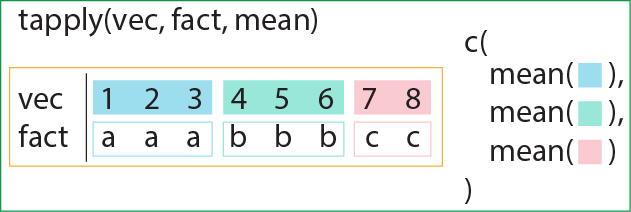
\includegraphics{././image/chapter15_tapply.png}

}

\caption{図6:tsapply関数の使い方}

\end{figure}

\begin{Shaded}
\begin{Highlighting}[]
\NormalTok{v }\OtherTok{\textless{}{-}} \DecValTok{1}\SpecialCharTok{:}\DecValTok{10}
\NormalTok{cutv }\OtherTok{\textless{}{-}} \FunctionTok{factor}\NormalTok{(}\FunctionTok{c}\NormalTok{(}\DecValTok{1}\NormalTok{, }\DecValTok{1}\NormalTok{, }\DecValTok{1}\NormalTok{, }\DecValTok{1}\NormalTok{, }\DecValTok{2}\NormalTok{, }\DecValTok{2}\NormalTok{, }\DecValTok{2}\NormalTok{, }\DecValTok{3}\NormalTok{, }\DecValTok{3}\NormalTok{, }\DecValTok{4}\NormalTok{))}
\FunctionTok{tapply}\NormalTok{(v, cutv, sum) }\CommentTok{\# ベクターを因子で切り分け、関数を適用する}
\end{Highlighting}
\end{Shaded}

\begin{verbatim}
 1  2  3  4 
10 18 17 10 
\end{verbatim}

\hypertarget{sweepux95a2ux6570}{%
\subsection{sweep関数}\label{sweepux95a2ux6570}}

sweep関数は、apply関数に似ていますが、第三引数が関数ではなく、ベクターであるところが異なります。MARGINは1が行方向、2が列方向であるのはapply関数と同じですが、第三引数が引き算に使われるのが特徴です。

\begin{Shaded}
\begin{Highlighting}[]
\FunctionTok{matrix}\NormalTok{(}\DecValTok{1}\SpecialCharTok{:}\DecValTok{15}\NormalTok{, }\AttributeTok{nrow=}\DecValTok{3}\NormalTok{)}
\end{Highlighting}
\end{Shaded}

\begin{verbatim}
     [,1] [,2] [,3] [,4] [,5]
[1,]    1    4    7   10   13
[2,]    2    5    8   11   14
[3,]    3    6    9   12   15
\end{verbatim}

\begin{Shaded}
\begin{Highlighting}[]
\FunctionTok{sweep}\NormalTok{(}\FunctionTok{matrix}\NormalTok{(}\DecValTok{1}\SpecialCharTok{:}\DecValTok{15}\NormalTok{, }\AttributeTok{nrow=}\DecValTok{3}\NormalTok{), }\DecValTok{1}\NormalTok{, }\DecValTok{1}\SpecialCharTok{:}\DecValTok{3}\NormalTok{) }\CommentTok{\# 行方向に1, 2, 3を引く}
\end{Highlighting}
\end{Shaded}

\begin{verbatim}
     [,1] [,2] [,3] [,4] [,5]
[1,]    0    3    6    9   12
[2,]    0    3    6    9   12
[3,]    0    3    6    9   12
\end{verbatim}

\begin{Shaded}
\begin{Highlighting}[]
\FunctionTok{sweep}\NormalTok{(}\FunctionTok{matrix}\NormalTok{(}\DecValTok{1}\SpecialCharTok{:}\DecValTok{15}\NormalTok{, }\AttributeTok{nrow=}\DecValTok{3}\NormalTok{), }\DecValTok{2}\NormalTok{, }\DecValTok{1}\SpecialCharTok{:}\DecValTok{5}\NormalTok{) }\CommentTok{\# 列方向に1, 2, 3, 4, 5を引く}
\end{Highlighting}
\end{Shaded}

\begin{verbatim}
     [,1] [,2] [,3] [,4] [,5]
[1,]    0    2    4    6    8
[2,]    1    3    5    7    9
[3,]    2    4    6    8   10
\end{verbatim}

\hypertarget{aggregateux95a2ux6570}{%
\subsection{aggregate関数}\label{aggregateux95a2ux6570}}

\textbf{aggregate関数}は、dplyrが出てくるまではデータフレームの結果を集計するのによく用いられてきた関数です。aggregate関数の第一引数は関数、第二引数にはby(因子のリスト)、第三引数に関数を取ります。aggregate関数はbyに指定した因子に従い、各列に関数を適用します。因子にカテゴリ(下の例ではirisの種、Species)を指定することで、因子ごとにデータを集計するのに用いることができます。

aggregate関数は引数にデータフレームだけでなく、\textbf{formula(式)}というものを取ることもできます。このformulaはRでは統計でよく用いられる表現で、\textsubscript{(チルダ)を演算子として用いるものです。\textbf{\textasciitilde の左側には従属変数、右側には独立変数を足し算・掛け算で記入する}形をとるのが最も一般的です。aggregate関数では、左側に関数を適用する列名、右側にbyにあたる因子を指定します。また、formulaでは、}の左側または右側に.(ピリオド)を置くことがあります。このピリオドは、「従属変数または独立変数に使用しなかったすべての列」を表す表現です。このformulaについては、統計の章で詳しく説明します。

\textbf{by関数}もaggregate関数と類似した関数ですが、byは関数の引数に各列のベクターではなく、因子で区切ったデータフレームを指定します。ですので、データフレームを処理できない関数を用いると、計算ができない場合があります。

\begin{figure}

{\centering 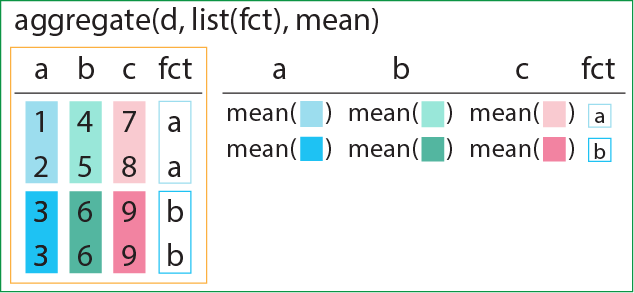
\includegraphics{././image/chapter15_aggregate.png}

}

\caption{図7:aggregate関数の使い方}

\end{figure}

\begin{Shaded}
\begin{Highlighting}[]
\FunctionTok{aggregate}\NormalTok{(iris[,}\DecValTok{1}\SpecialCharTok{:}\DecValTok{4}\NormalTok{], }\AttributeTok{by=}\FunctionTok{list}\NormalTok{(iris}\SpecialCharTok{$}\NormalTok{Species), }\AttributeTok{FUN =} \StringTok{"mean"}\NormalTok{) }\CommentTok{\# byはリスト}
\end{Highlighting}
\end{Shaded}

\begin{verbatim}
     Group.1 Sepal.Length Sepal.Width Petal.Length Petal.Width
1     setosa        5.006       3.428        1.462       0.246
2 versicolor        5.936       2.770        4.260       1.326
3  virginica        6.588       2.974        5.552       2.026
\end{verbatim}

\begin{Shaded}
\begin{Highlighting}[]
\FunctionTok{aggregate}\NormalTok{(iris[,}\DecValTok{1}\SpecialCharTok{:}\DecValTok{4}\NormalTok{], }\AttributeTok{by=}\FunctionTok{list}\NormalTok{(iris}\SpecialCharTok{$}\NormalTok{Species), }\AttributeTok{FUN =} \StringTok{"min"}\NormalTok{)}
\end{Highlighting}
\end{Shaded}

\begin{verbatim}
     Group.1 Sepal.Length Sepal.Width Petal.Length Petal.Width
1     setosa          4.3         2.3          1.0         0.1
2 versicolor          4.9         2.0          3.0         1.0
3  virginica          4.9         2.2          4.5         1.4
\end{verbatim}

\begin{Shaded}
\begin{Highlighting}[]
\FunctionTok{head}\NormalTok{(Species)}
\end{Highlighting}
\end{Shaded}

\begin{verbatim}
Error in eval(expr, envir, enclos): object 'Species' not found
\end{verbatim}

\begin{Shaded}
\begin{Highlighting}[]
\FunctionTok{aggregate}\NormalTok{(.}\SpecialCharTok{\textasciitilde{}}\NormalTok{Species, }\AttributeTok{data =}\NormalTok{ iris, max)}
\end{Highlighting}
\end{Shaded}

\begin{verbatim}
     Species Sepal.Length Sepal.Width Petal.Length Petal.Width
1     setosa          5.8         4.4          1.9         0.6
2 versicolor          7.0         3.4          5.1         1.8
3  virginica          7.9         3.8          6.9         2.5
\end{verbatim}

\begin{Shaded}
\begin{Highlighting}[]
\FunctionTok{head}\NormalTok{(ToothGrowth)}
\end{Highlighting}
\end{Shaded}

\begin{verbatim}
   len supp dose
1  4.2   VC  0.5
2 11.5   VC  0.5
3  7.3   VC  0.5
4  5.8   VC  0.5
5  6.4   VC  0.5
6 10.0   VC  0.5
\end{verbatim}

\begin{Shaded}
\begin{Highlighting}[]
\FunctionTok{aggregate}\NormalTok{(len}\SpecialCharTok{\textasciitilde{}}\NormalTok{., }\AttributeTok{data =}\NormalTok{ ToothGrowth, mean)}
\end{Highlighting}
\end{Shaded}

\begin{verbatim}
  supp dose   len
1   OJ  0.5 13.23
2   VC  0.5  7.98
3   OJ  1.0 22.70
4   VC  1.0 16.77
5   OJ  2.0 26.06
6   VC  2.0 26.14
\end{verbatim}

\begin{Shaded}
\begin{Highlighting}[]
\FunctionTok{by}\NormalTok{(iris[, }\DecValTok{1}\NormalTok{], }\FunctionTok{list}\NormalTok{(iris}\SpecialCharTok{$}\NormalTok{Species), mean)}
\end{Highlighting}
\end{Shaded}

\begin{verbatim}
: setosa
[1] 5.006
------------------------------------------------------------ 
: versicolor
[1] 5.936
------------------------------------------------------------ 
: virginica
[1] 6.588
\end{verbatim}

\begin{Shaded}
\begin{Highlighting}[]
\FunctionTok{by}\NormalTok{(iris[, }\DecValTok{1}\SpecialCharTok{:}\DecValTok{2}\NormalTok{], }\FunctionTok{list}\NormalTok{(iris}\SpecialCharTok{$}\NormalTok{Species), mean) }\CommentTok{\# meanは2列のデータを処理できない}
\end{Highlighting}
\end{Shaded}

\begin{verbatim}
Warning in mean.default(data[x, , drop = FALSE], ...): argument is not numeric
or logical: returning NA

Warning in mean.default(data[x, , drop = FALSE], ...): argument is not numeric
or logical: returning NA

Warning in mean.default(data[x, , drop = FALSE], ...): argument is not numeric
or logical: returning NA
\end{verbatim}

\begin{verbatim}
: setosa
[1] NA
------------------------------------------------------------ 
: versicolor
[1] NA
------------------------------------------------------------ 
: virginica
[1] NA
\end{verbatim}

\begin{Shaded}
\begin{Highlighting}[]
\FunctionTok{by}\NormalTok{(iris[, }\DecValTok{1}\SpecialCharTok{:}\DecValTok{4}\NormalTok{], }\FunctionTok{list}\NormalTok{(iris}\SpecialCharTok{$}\NormalTok{Species), summary) }\CommentTok{\# summaryはデータフレームを引数にできるので、計算できる}
\end{Highlighting}
\end{Shaded}

\begin{verbatim}
: setosa
  Sepal.Length    Sepal.Width     Petal.Length    Petal.Width   
 Min.   :4.300   Min.   :2.300   Min.   :1.000   Min.   :0.100  
 1st Qu.:4.800   1st Qu.:3.200   1st Qu.:1.400   1st Qu.:0.200  
 Median :5.000   Median :3.400   Median :1.500   Median :0.200  
 Mean   :5.006   Mean   :3.428   Mean   :1.462   Mean   :0.246  
 3rd Qu.:5.200   3rd Qu.:3.675   3rd Qu.:1.575   3rd Qu.:0.300  
 Max.   :5.800   Max.   :4.400   Max.   :1.900   Max.   :0.600  
------------------------------------------------------------ 
: versicolor
  Sepal.Length    Sepal.Width     Petal.Length   Petal.Width   
 Min.   :4.900   Min.   :2.000   Min.   :3.00   Min.   :1.000  
 1st Qu.:5.600   1st Qu.:2.525   1st Qu.:4.00   1st Qu.:1.200  
 Median :5.900   Median :2.800   Median :4.35   Median :1.300  
 Mean   :5.936   Mean   :2.770   Mean   :4.26   Mean   :1.326  
 3rd Qu.:6.300   3rd Qu.:3.000   3rd Qu.:4.60   3rd Qu.:1.500  
 Max.   :7.000   Max.   :3.400   Max.   :5.10   Max.   :1.800  
------------------------------------------------------------ 
: virginica
  Sepal.Length    Sepal.Width     Petal.Length    Petal.Width   
 Min.   :4.900   Min.   :2.200   Min.   :4.500   Min.   :1.400  
 1st Qu.:6.225   1st Qu.:2.800   1st Qu.:5.100   1st Qu.:1.800  
 Median :6.500   Median :3.000   Median :5.550   Median :2.000  
 Mean   :6.588   Mean   :2.974   Mean   :5.552   Mean   :2.026  
 3rd Qu.:6.900   3rd Qu.:3.175   3rd Qu.:5.875   3rd Qu.:2.300  
 Max.   :7.900   Max.   :3.800   Max.   :6.900   Max.   :2.500  
\end{verbatim}

\bookmarksetup{startatroot}

\hypertarget{tidyrdplyr}{%
\chapter{tidyr・dplyr}\label{tidyrdplyr}}

データを取得し,そのデータをそのまま統計に用いることができることは稀です.データ解析では,データの整理整頓(data
wrangling)に多くの時間が割かれています.データの整理整頓には,様々なツールが用いられます.前述のapply関数群もデータの要約等の整理整頓に用いることができます.

ただし,前章で説明した通り,apply関数群は関数ごとに引数の順序や引数に与えるデータ型などが異なっており,使い勝手がよいとは言えません.同様の機能を持つ\href{https://cran.r-project.org/web/packages/plyr/index.html}{plyrパッケージ}というライブラリもありますが,やはり使い勝手が良くなかったため,それほど用いられていません.

現在では,これらの関数・ライブラリに代わり,データの整理整頓には\textbf{tidyr・dplyr}を用いるのがRでは事実上のデフォルトとなっています.tidyr・dplyrの特徴は以下の通りです.

\begin{itemize}
\tightlist
\item
  \textbf{パイプ演算子}を用いることを前提として関数が設計されている
\item
  第一引数にはデータフレームを取り,データフレームを加工する
\item
  出力もデータフレーム(正確にはtibble)で統一されている
\end{itemize}

tidyr・dplyrを用いることで,パイプ演算子を活用し,余計な変数を作ることなく,データフレームを自由自在に取り扱うことができます.

\hypertarget{ux30e1ux30bdux30c3ux30c9ux30c1ux30a7ux30fcux30f3}{%
\section{メソッドチェーン}\label{ux30e1ux30bdux30c3ux30c9ux30c1ux30a7ux30fcux30f3}}

tidyr・dplyrについて説明する前に,R以外の言語で用いられている,\textbf{メソッドチェーン}について簡単に説明します.

R以外の言語では,オブジェクトに対して演算を行う時,関数以外に\textbf{メソッド}を利用することがあります.メソッドは,オブジェクトの後にピリオドで繋いで,オブジェクトに何らかの演算を行うものです.例えばRubyでは文字列に対して,「.upcase」というメソッドが設定されています..upcaseは文字列を大文字にするメソッドです.例えば「``Hello
world''.upcase」とすると,``Hello
world''の小文字が大文字に変換され,``HELLO WORLD''が返ってきます.

このメソッドは2つ以上繋げて用いることができます.例えば,.reverseは文字列を逆順にするメソッドですが,「``Hello
world''.reverse.upcase」とすると,``Hello
world''を逆順にし,続いて大文字に変換することができます.このように,メソッドを繋いで使用することをメソッドチェーンと呼びます.

以下に,Rubyとjavascriptでのメソッドチェーンの例を示します.

\textbf{Rubyでのメソッドチェーン}

\begin{Shaded}
\begin{Highlighting}[]
\NormalTok{string }\KeywordTok{=} \StringTok{"dlrow olleH"}
\NormalTok{string}\AttributeTok{.reverse.upcase} \CommentTok{\# 文字列を逆順にし,大文字に変換する}
\CommentTok{\#\textgreater{}  "HELLO WORLD"}
\end{Highlighting}
\end{Shaded}

\textbf{JavaScriptでのメソッドチェーン}

\begin{Shaded}
\begin{Highlighting}[]
\KeywordTok{var}\NormalTok{ firstName }\OperatorTok{=} \StringTok{" Rajat "}\OperatorTok{;} \CommentTok{// firstNameは" Rajat "}
\BuiltInTok{console}\OperatorTok{.}\FunctionTok{log}\NormalTok{(firstName)}\OperatorTok{;} 
\NormalTok{\#}\OperatorTok{\textgreater{}} \StringTok{"Rajat"}
\KeywordTok{var}\NormalTok{ modifiedName }\OperatorTok{=} 
\NormalTok{  firstName }
    \OperatorTok{.}\FunctionTok{toUpperCase}\NormalTok{() }\CommentTok{// 大文字にして}
        \OperatorTok{.}\FunctionTok{trim}\NormalTok{()}\OperatorTok{;} \CommentTok{// 前後のスペースを削除する}
\BuiltInTok{console}\OperatorTok{.}\FunctionTok{log}\NormalTok{(modifiedName)}
\NormalTok{\#}\OperatorTok{\textgreater{}} \StringTok{"RAJAT"}
\end{Highlighting}
\end{Shaded}

メソッドチェーンのよいところは,\textbf{演算の過程を左から右へ,文章を読むように追いかけることができる}ことです.上記のメソッドチェーンと同じような演算をRで行うと,以下のようになります.

\begin{Shaded}
\begin{Highlighting}[]
\NormalTok{pacman}\SpecialCharTok{::}\FunctionTok{p\_load}\NormalTok{(tidyverse) }\CommentTok{\# stringrを使うためtidyverseをロードする}
\NormalTok{firstname }\OtherTok{\textless{}{-}} \StringTok{" Rajat "}

\CommentTok{\# 例1}
\FunctionTok{str\_to\_upper}\NormalTok{(}\FunctionTok{str\_trim}\NormalTok{(firstname)) }\CommentTok{\# スペースを取り除いて大文字にする}
\end{Highlighting}
\end{Shaded}

\begin{verbatim}
[1] "RAJAT"
\end{verbatim}

\begin{Shaded}
\begin{Highlighting}[]
\CommentTok{\# 例2}
\NormalTok{firstname1 }\OtherTok{\textless{}{-}} \FunctionTok{str\_trim}\NormalTok{(firstname) }\CommentTok{\# スペースを取り除く}
\FunctionTok{str\_to\_upper}\NormalTok{(firstname1) }\CommentTok{\# 大文字にする}
\end{Highlighting}
\end{Shaded}

\begin{verbatim}
[1] "RAJAT"
\end{verbatim}

Rではメソッドチェーンは使えないので,複数の演算を行うときには,上の例1のように関数の中に関数を入れる(ネストする)か,例2のように一時的に計算結果を変数に入れておき,その一時的な変数を利用して再度演算(逐次的な演算)をする必要があります.

どちらも実用上大きな問題ないのですが,プログラムとしては理解しにくく,メソッドチェーンのように簡単に複数の処理を行えるものではありません.

このような問題を解決する演算子が,\textbf{パイプ演算子}です.

\hypertarget{ux30d1ux30a4ux30d7ux6f14ux7b97ux5b50pipe-operator}{%
\section{パイプ演算子(pipe
operator)}\label{ux30d1ux30a4ux30d7ux6f14ux7b97ux5b50pipe-operator}}

パイプ演算子とは,\textbf{「演算子の前のオブジェクトを,演算子の後ろの関数の引数にする」}演算子です.Rのパイプ演算子には以下の2種類があります.

\begin{itemize}
\tightlist
\item
  \textbf{\textbar\textgreater{}}:Rのデフォルトのパイプ演算子
\item
  \textbf{\%\textgreater\%}:magrittrパッケージに登録されているパイプ演算子
\end{itemize}

パイプ演算子を用いると,以下の演算は同じ意味を持ちます.

\begin{Shaded}
\begin{Highlighting}[]
\NormalTok{vec }\OtherTok{\textless{}{-}} \FunctionTok{c}\NormalTok{(}\DecValTok{1}\NormalTok{, }\DecValTok{2}\NormalTok{, }\DecValTok{3}\NormalTok{)}
\FunctionTok{mean}\NormalTok{(vec) }\CommentTok{\# 通常の演算}
\end{Highlighting}
\end{Shaded}

\begin{verbatim}
[1] 2
\end{verbatim}

\begin{Shaded}
\begin{Highlighting}[]
\NormalTok{vec }\SpecialCharTok{|\textgreater{}} \FunctionTok{mean}\NormalTok{() }\CommentTok{\# パイプ演算子}
\end{Highlighting}
\end{Shaded}

\begin{verbatim}
[1] 2
\end{verbatim}

これだけ見てもパイプ演算子を用いる利点はよくわかりませんが,パイプ演算子を用いることで,上記のメソッドチェーンのような機能をRに与えることができます.

上のjavascriptでのメソッドチェーンと同じ演算をパイプ演算子を用いて行うと,以下のようになります.パイプ演算子を用いることで,「文字列からスペースを取り除き,大文字にする」という,文章と同じ順序でデータを処理することができます.このように順序が変わることで,一度にたくさんの演算を行っても,理解しやすいプログラムを書くことができます.

\begin{Shaded}
\begin{Highlighting}[]
\NormalTok{firstname }\OtherTok{\textless{}{-}} \StringTok{" Rajat "}
\NormalTok{firstname }\SpecialCharTok{|\textgreater{}} \FunctionTok{str\_trim}\NormalTok{() }\SpecialCharTok{|\textgreater{}} \FunctionTok{str\_to\_upper}\NormalTok{() }\CommentTok{\# スペースを取り除き,大文字にする}
\end{Highlighting}
\end{Shaded}

\begin{verbatim}
[1] "RAJAT"
\end{verbatim}

\hypertarget{ux30c7ux30d5ux30a9ux30ebux30c8ux3068magrittrux30d1ux30c3ux30b1ux30fcux30b8ux306eux30d1ux30a4ux30d7ux6f14ux7b97ux5b50}{%
\subsection{デフォルトとmagrittrパッケージのパイプ演算子}\label{ux30c7ux30d5ux30a9ux30ebux30c8ux3068magrittrux30d1ux30c3ux30b1ux30fcux30b8ux306eux30d1ux30a4ux30d7ux6f14ux7b97ux5b50}}

では,まず2種類のパイプ演算子について見ていきましょう.Rで先に実装されたのはmagrittrで,2014年にライブラリが公開されています.Rのデフォルトのパイプ演算子はずっと後になって,2021年にR
version 4.1.0で実装されました.

Rstudioでは,パイプ演算子を「\textbf{Ctrl+Shift+M}」のショートカットで入力することができます.RStudioはRのデフォルトのパイプ演算子が実装される前から存在するため,デフォルトのパイプ演算子はmagrittrの「\%\textgreater\%」になっています.デフォルトのパイプ演算子をRのデフォルトのもの(\textbar\textgreater)に変更する場合には,「Tools→Global
Options」から「Code」を選択し,下の図1の赤線で囲った部分にチェックを入れます.

\begin{figure}

{\centering 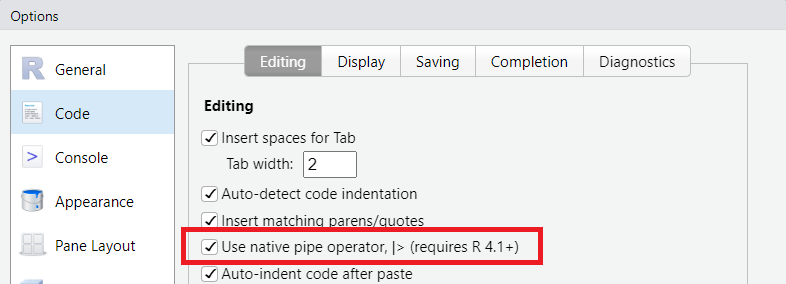
\includegraphics{././image/chapter16_pipe_shortcut.png}

}

\caption{図2:ショートカットで入力するパイプ演算子を変更する}

\end{figure}

2種類のパイプ演算子は,記号が異なるだけでなく,使い方も少し異なっています.

\begin{itemize}
\tightlist
\item
  関数の後の()の必要性(\textbar\textgreater は必要,\%\textgreater\%は不必要)
\item
  引数の位置を指定する文字の違い(\textbar\textgreater は「\_」(アンダースコア),\%\textgreater\%は「.」(ピリオド))
\item
  関数のreturnに使えるかどうか(\textbar\textgreater は使えず,\%\textgreater\%は使える)
\end{itemize}

また,\%\textgreater\%を用いるのにはmagrittrパッケージ(tidyverseに含まれている)をロードする必要があるのに対し,\textbar\textgreater はライブラリのロードを必要としません.

\hypertarget{ux95a2ux6570ux306eux30abux30c3ux30b3ux306eux6709ux7121}{%
\subsubsection{関数のカッコの有無}\label{ux95a2ux6570ux306eux30abux30c3ux30b3ux306eux6709ux7121}}

\textbar\textgreater では関数名の後にカッコをつけるのが必須で,カッコが無いとエラーが出ます.

\textbf{パイプ演算子}

\begin{Shaded}
\begin{Highlighting}[]
\NormalTok{pacman}\SpecialCharTok{::}\FunctionTok{p\_load}\NormalTok{(tidyverse) }\CommentTok{\# magrittrはtidyverseに含まれる}

\NormalTok{func1 }\OtherTok{\textless{}{-}} \ControlFlowTok{function}\NormalTok{(x, }\AttributeTok{y =} \DecValTok{1}\NormalTok{)\{x }\SpecialCharTok{+}\NormalTok{ y\} }\CommentTok{\# xに1を足す関数}

\FunctionTok{func1}\NormalTok{(}\DecValTok{1}\NormalTok{) }\CommentTok{\# 2が帰ってくる}
\end{Highlighting}
\end{Shaded}

\begin{verbatim}
[1] 2
\end{verbatim}

\begin{Shaded}
\begin{Highlighting}[]
\DecValTok{1} \SpecialCharTok{|\textgreater{}} \FunctionTok{func1}\NormalTok{() }\CommentTok{\# |\textgreater{}ではカッコが必須}
\end{Highlighting}
\end{Shaded}

\begin{verbatim}
[1] 2
\end{verbatim}

\begin{Shaded}
\begin{Highlighting}[]
\DecValTok{1} \SpecialCharTok{|\textgreater{}}\NormalTok{ func1 }\CommentTok{\# カッコが無いとエラー}
\end{Highlighting}
\end{Shaded}

\begin{verbatim}
Error: The pipe operator requires a function call as RHS (<text>:1:6)
\end{verbatim}

\%\textgreater\%では,カッコがあってもなくても計算をしてくれます.

\begin{Shaded}
\begin{Highlighting}[]
\DecValTok{1} \SpecialCharTok{\%\textgreater{}\%} \FunctionTok{func1}\NormalTok{() }\CommentTok{\# \%\textgreater{}\%はカッコがあってもなくても計算できる}
\end{Highlighting}
\end{Shaded}

\begin{verbatim}
[1] 2
\end{verbatim}

\begin{Shaded}
\begin{Highlighting}[]
\DecValTok{1} \SpecialCharTok{\%\textgreater{}\%}\NormalTok{ func1}
\end{Highlighting}
\end{Shaded}

\begin{verbatim}
[1] 2
\end{verbatim}

\textbar\textgreater では,パイプ演算子の前の値を代入する位置をアンダースコア(\_)で指定できます.\%\textgreater\%では,ピリオド(.)で指定します.指定しない場合には,パイプ演算子の前の値が第一引数となります.

\begin{Shaded}
\begin{Highlighting}[]
\FunctionTok{func1}\NormalTok{(}\DecValTok{1}\NormalTok{, }\DecValTok{2}\NormalTok{) }\CommentTok{\# 引数を2個取り,足し算する関数}
\end{Highlighting}
\end{Shaded}

\begin{verbatim}
[1] 3
\end{verbatim}

\begin{Shaded}
\begin{Highlighting}[]
\DecValTok{1} \SpecialCharTok{|\textgreater{}} \FunctionTok{func1}\NormalTok{(}\AttributeTok{y =} \DecValTok{2}\NormalTok{) }\CommentTok{\# 第一引数に1が入る(第2引数が2)}
\end{Highlighting}
\end{Shaded}

\begin{verbatim}
[1] 3
\end{verbatim}

\begin{Shaded}
\begin{Highlighting}[]
\DecValTok{2} \SpecialCharTok{|\textgreater{}} \FunctionTok{func1}\NormalTok{(}\AttributeTok{x =} \DecValTok{1}\NormalTok{, }\AttributeTok{y =}\NormalTok{ \_) }\CommentTok{\# 引数を入る位置を「\_」で指定}
\end{Highlighting}
\end{Shaded}

\begin{verbatim}
[1] 3
\end{verbatim}

\begin{Shaded}
\begin{Highlighting}[]
\DecValTok{1} \SpecialCharTok{\%\textgreater{}\%} \FunctionTok{func1}\NormalTok{(}\AttributeTok{y =} \DecValTok{2}\NormalTok{) }\CommentTok{\# 第一引数に1が入る}
\end{Highlighting}
\end{Shaded}

\begin{verbatim}
[1] 3
\end{verbatim}

\begin{Shaded}
\begin{Highlighting}[]
\DecValTok{2} \SpecialCharTok{\%\textgreater{}\%} \FunctionTok{func1}\NormalTok{(}\AttributeTok{x =} \DecValTok{1}\NormalTok{, }\AttributeTok{y =}\NormalTok{ .) }\CommentTok{\# 引数を入る位置を「.」で指定}
\end{Highlighting}
\end{Shaded}

\begin{verbatim}
[1] 3
\end{verbatim}

\textbar\textgreater・\%\textgreater\%のどちらでも,ピリオドやアンダースコアにインデックス・列名を付け加えることで,要素を呼び出すことができます.

\begin{Shaded}
\begin{Highlighting}[]
\DecValTok{4}\SpecialCharTok{:}\DecValTok{6} \SpecialCharTok{|\textgreater{}}\NormalTok{ \_[}\DecValTok{2}\NormalTok{] }\CommentTok{\# インデックスで呼び出せる}
\end{Highlighting}
\end{Shaded}

\begin{verbatim}
[1] 5
\end{verbatim}

\begin{Shaded}
\begin{Highlighting}[]
\DecValTok{4}\SpecialCharTok{:}\DecValTok{6} \SpecialCharTok{\%\textgreater{}\%}\NormalTok{ .[}\DecValTok{2}\NormalTok{]}
\end{Highlighting}
\end{Shaded}

\begin{verbatim}
[1] 5
\end{verbatim}

\begin{Shaded}
\begin{Highlighting}[]
\NormalTok{iris }\SpecialCharTok{|\textgreater{}}\NormalTok{ \_}\SpecialCharTok{$}\NormalTok{Species }\SpecialCharTok{|\textgreater{}} \FunctionTok{head}\NormalTok{() }\CommentTok{\# 列名で呼び出せる}
\end{Highlighting}
\end{Shaded}

\begin{verbatim}
[1] setosa setosa setosa setosa setosa setosa
Levels: setosa versicolor virginica
\end{verbatim}

\begin{Shaded}
\begin{Highlighting}[]
\NormalTok{iris }\SpecialCharTok{\%\textgreater{}\%}\NormalTok{ .}\SpecialCharTok{$}\NormalTok{Species }\SpecialCharTok{\%\textgreater{}\%}\NormalTok{ head}
\end{Highlighting}
\end{Shaded}

\begin{verbatim}
[1] setosa setosa setosa setosa setosa setosa
Levels: setosa versicolor virginica
\end{verbatim}

\textbar\textgreater も\%\textgreater\%も共に,演算子の後に改行を入れることができます.パイプ演算子を用いるときには,以下のような書き方をするのが一般的です.

\begin{Shaded}
\begin{Highlighting}[]
\StringTok{"Hello world"} \SpecialCharTok{|\textgreater{}} \CommentTok{\# 文字列を}
  \FunctionTok{str\_replace}\NormalTok{(}\AttributeTok{pattern =} \StringTok{"world"}\NormalTok{, }\AttributeTok{replacement =} \StringTok{"R"}\NormalTok{) }\SpecialCharTok{|\textgreater{}} \CommentTok{\# 一部置き換え,}
  \FunctionTok{str\_to\_upper}\NormalTok{() }\CommentTok{\# 大文字にする}
\end{Highlighting}
\end{Shaded}

\begin{verbatim}
[1] "HELLO R"
\end{verbatim}

\hypertarget{tidy-data}{%
\section{tidy data}\label{tidy-data}}

tidyr・dplyrの説明の前に,データフレームを取り扱う上で重要な概念である,\textbf{「tidy
data(整然としたデータ)」}について簡単に説明します.

「\href{https://r4ds.hadley.nz/data-tidy.html}{tidy
data}」はggplot2やtidyr,dplyrを開発しているPOSIT
SoftwareのチーフサイエンティストであるHadley
Wickhamが2014年に示したデータ構造の考え方です.データフレームのような表形式のデータを対象としたもので,\textbf{「データの行は各観察結果,データの列は各列が一つの種類のデータであるように整理し,データの各要素には一つの値しか入力しない」}というルールに従い,データは準備されるべきであるとしています.tidyr,dplyrはこの概念を念頭に設計されています.

tidyではないデータは世の中にゴロゴロ転がっています.以下の表1はファイザーの\href{https://www.nejm.org/doi/pdf/10.1056/NEJMoa2034577?articleTools=true}{COVID-19ワクチン(コミナティ筋注)の第3相試験に関するNew
England Journal of Medicineの論文}の表1の一部を加工したものです.

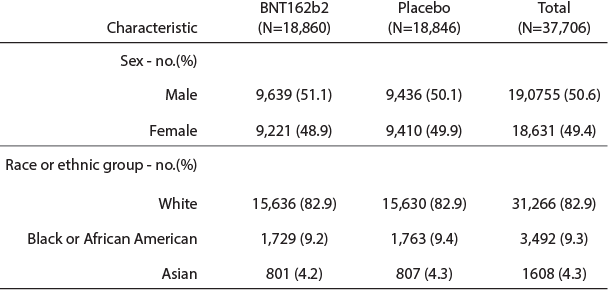
\includegraphics{././image/chapter16_nontidy.png}

論文の表は人が見やすいように作成されています.ですので,この表を見て,意味が全くわからない,ということはあまりないでしょう.しかし,この表はtidyではありません.

まず,1つのセル(要素)に人数とその割合(\%)が記載されています.また,投薬された治験薬(BNT162b2とPlacebo)は処置(Treatment)という同じカテゴリのデータですので,列名として2つに分けていることで,同じカテゴリのデータを2列に表示していることになっています.上の2行は性別に関するデータ,下の3行は人種に関するデータですので,2つの別のデータが同じ表に乗っています.したがって,この表は人にとってはわかりやすくても,tidyなデータではありません.

上の表をtidyなデータにしたものが,以下の表2です.人数のデータ,割合のデータは各1列に,治験薬はTreatmentとして1列に表記しています.性別と人種ではデータのカテゴリが異なりますので,表を2つに分けています.Ratioはそのまま変換すると足し合わせが200\%となるため,2で割って調整しています.

これが完全なtidyかと言われるとやや難しいところもありますが,少なくとも上の表1よりはRで取り扱いしやすいデータとなっています.

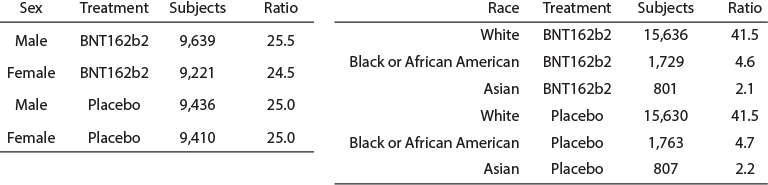
\includegraphics{././image/chapter16_tidy.png}

Rでは,グラフ作成・統計共に,元の表より下のtidyなデータの方が取り扱いやすくなります.多くのデータは人が見やすいように収集・準備されており,tidyではありません.R上でデータをtidyに加工・整形するためのツールが,\textbf{tidyrとdplyr}です.

\hypertarget{tidyr}{%
\subsection{tidyr}\label{tidyr}}

\textbf{tidyr}はデータを\textbf{縦持ち・横持ち}に変換するためのライブラリです.この縦持ち・横持ちというのは,以下の図のように,縦長・横長のデータのことを指します.

人が見る分には,横持ちのデータはわかりやすく,理解に特に問題は感じません.しかし,Rで取り扱う場合には,圧倒的に縦持ちのデータの方が取り扱いが簡単です.ですので,人が作ったデータをRで取り扱うために縦持ちに変換する,Rで生成したデータを人が理解しやすいように横持ちに変換する時に,tidyrの関数を用いることになります.以下の表3にtidyrの関数の一覧を示します.

\href{https://rstudio.github.io/cheatsheets/tidyr.pdf}{これ}を参照

\begin{longtable}[]{@{}ll@{}}
\caption{表3:tidyrの関数群}\tabularnewline
\toprule()
関数名 & 適用する演算 \\
\midrule()
\endfirsthead
\toprule()
関数名 & 適用する演算 \\
\midrule()
\endhead
pivot\_longer & データフレームを縦持ちデータにする \\
gather & データフレームを縦持ちデータにする(旧版) \\
pivot\_wider & データフレームを横持ちデータにする \\
spread & データフレームを横持ちデータにする(旧版) \\
group\_by & データを列でグループ化する \\
nest & データをネストする \\
unnest & ネストを解除する \\
drop\_na & NAを含む行を取り除く(na.omitと同じ) \\
expand & 各列の組み合わせを作成する \\
fill & NAに上の要素を埋める \\
replace\_na & NAに引数で指定した要素を埋める \\
\bottomrule()
\end{longtable}

\hypertarget{pivot_longerux3068pivot_wider}{%
\subsection{pivot\_longerとpivot\_wider}\label{pivot_longerux3068pivot_wider}}

データフレームを縦持ちに変換する関数が\textbf{pivot\_longer関数},横持ちに変換する関数が\textbf{pivot\_wider関数}です.共に第一引数がデータフレームで,パイプ演算子を用いて演算を行うのが一般的です.

pivot\_longer関数もpivot\_wider関数も,Rでのデータ解析ではとても重要となりますが,共に変換がやや複雑で,挙動がわかりにくい関数でもあります.下の例を参考に,どのようにデータが変換されるのか,よく理解した上で用いるのがよいでしょう.

\hypertarget{ux7e26ux6301ux3061ux3078ux306eux5909ux63dbpivot_longer}{%
\subsubsection{縦持ちへの変換:pivot\_longer}\label{ux7e26ux6301ux3061ux3078ux306eux5909ux63dbpivot_longer}}

\textbf{pivot\_longer関数}はデータフレームと列番号を引数に取り,列番号で指定した列の名前をnameという列の要素に変換し,列番号で指定した列の要素をvalueという名前の列として,1列のデータに変換します.このような変換により,データは縦長の構造を取ります.

変換後の列名は引数で指定でき,列の名前に関する列名は「names\_to」,列の要素に関する列名は「values\_to」引数に指定します.このpivot\_longer関数は特に統計・グラフ作成の際によく用います.

tidyrが開発されるまでは,reshapeという関数で縦持ち変換を行うのが一般的でした.また,pivot\_longer関数はtidyr開発初期にはgatherという名前で,引数の順番も少し異なっていました.今でもreshapeやgatherを用いて縦持ちへの変換を行うことはできます.

\begin{Shaded}
\begin{Highlighting}[]
\FunctionTok{head}\NormalTok{(iris)}
\end{Highlighting}
\end{Shaded}

\begin{verbatim}
  Sepal.Length Sepal.Width Petal.Length Petal.Width Species
1          5.1         3.5          1.4         0.2  setosa
2          4.9         3.0          1.4         0.2  setosa
3          4.7         3.2          1.3         0.2  setosa
4          4.6         3.1          1.5         0.2  setosa
5          5.0         3.6          1.4         0.2  setosa
6          5.4         3.9          1.7         0.4  setosa
\end{verbatim}

\begin{Shaded}
\begin{Highlighting}[]
\CommentTok{\# pivot\_longer 縦持ちデータへの変換}
\NormalTok{iris }\SpecialCharTok{|\textgreater{}} \FunctionTok{pivot\_longer}\NormalTok{(}\AttributeTok{cols =} \DecValTok{1}\SpecialCharTok{:}\DecValTok{4}\NormalTok{) }
\end{Highlighting}
\end{Shaded}

\begin{verbatim}
# A tibble: 600 x 3
   Species name         value
   <fct>   <chr>        <dbl>
 1 setosa  Sepal.Length   5.1
 2 setosa  Sepal.Width    3.5
 3 setosa  Petal.Length   1.4
 4 setosa  Petal.Width    0.2
 5 setosa  Sepal.Length   4.9
 6 setosa  Sepal.Width    3  
 7 setosa  Petal.Length   1.4
 8 setosa  Petal.Width    0.2
 9 setosa  Sepal.Length   4.7
10 setosa  Sepal.Width    3.2
# i 590 more rows
\end{verbatim}

\begin{Shaded}
\begin{Highlighting}[]
\NormalTok{iris }\SpecialCharTok{|\textgreater{}} \FunctionTok{pivot\_longer}\NormalTok{(}\AttributeTok{cols =} \DecValTok{1}\SpecialCharTok{:}\DecValTok{4}\NormalTok{, }\AttributeTok{names\_to =} \StringTok{"category"}\NormalTok{, }\AttributeTok{values\_to =} \StringTok{"value"}\NormalTok{) }\CommentTok{\# 上と同じ(列名を設定)}
\end{Highlighting}
\end{Shaded}

\begin{verbatim}
# A tibble: 600 x 3
   Species category     value
   <fct>   <chr>        <dbl>
 1 setosa  Sepal.Length   5.1
 2 setosa  Sepal.Width    3.5
 3 setosa  Petal.Length   1.4
 4 setosa  Petal.Width    0.2
 5 setosa  Sepal.Length   4.9
 6 setosa  Sepal.Width    3  
 7 setosa  Petal.Length   1.4
 8 setosa  Petal.Width    0.2
 9 setosa  Sepal.Length   4.7
10 setosa  Sepal.Width    3.2
# i 590 more rows
\end{verbatim}

\begin{Shaded}
\begin{Highlighting}[]
\CommentTok{\# gather}
\NormalTok{iris }\SpecialCharTok{|\textgreater{}} \FunctionTok{gather}\NormalTok{(category, value, }\DecValTok{1}\SpecialCharTok{:}\DecValTok{4}\NormalTok{) }\SpecialCharTok{|\textgreater{}} \FunctionTok{head}\NormalTok{()}
\end{Highlighting}
\end{Shaded}

\begin{verbatim}
  Species     category value
1  setosa Sepal.Length   5.1
2  setosa Sepal.Length   4.9
3  setosa Sepal.Length   4.7
4  setosa Sepal.Length   4.6
5  setosa Sepal.Length   5.0
6  setosa Sepal.Length   5.4
\end{verbatim}

\begin{Shaded}
\begin{Highlighting}[]
\NormalTok{iris }\SpecialCharTok{|\textgreater{}} \FunctionTok{gather}\NormalTok{(category, value, }\SpecialCharTok{{-}}\NormalTok{Species) }\SpecialCharTok{|\textgreater{}} \FunctionTok{head}\NormalTok{() }\CommentTok{\# 上と同じ}
\end{Highlighting}
\end{Shaded}

\begin{verbatim}
  Species     category value
1  setosa Sepal.Length   5.1
2  setosa Sepal.Length   4.9
3  setosa Sepal.Length   4.7
4  setosa Sepal.Length   4.6
5  setosa Sepal.Length   5.0
6  setosa Sepal.Length   5.4
\end{verbatim}

\hypertarget{ux6a2aux6301ux3061ux3078ux306eux5909ux63dbpivot_wider}{%
\subsubsection{横持ちへの変換:pivot\_wider}\label{ux6a2aux6301ux3061ux3078ux306eux5909ux63dbpivot_wider}}

\textbf{pivot\_wider関数}は,データを横持ちに変換する関数です.pivot\_wider関数は列名となる列をnames\_from引数に,要素となる列をvalues\_from引数に指定します.指定しなかった列はそのまま維持されます.names\_fromで指定した列の要素は各列名となり,values\_fromで指定した列の要素がnames\_fromで新しく作られた列の値となります.この変換により,データは横長の,幅の広い構造を取ることになります.

横持ちへの変換もreshapeを用いて行うことができます.また,pivot\_widerは以前はspreadという名前であったため,このspread関数を用いて横持ちデータへの変換を行うこともできます.

\begin{Shaded}
\begin{Highlighting}[]
\CommentTok{\# pivot\_wider 横持ちデータへの変換}
\NormalTok{us\_rent\_income}
\end{Highlighting}
\end{Shaded}

\begin{verbatim}
# A tibble: 104 x 5
   GEOID NAME       variable estimate   moe
   <chr> <chr>      <chr>       <dbl> <dbl>
 1 01    Alabama    income      24476   136
 2 01    Alabama    rent          747     3
 3 02    Alaska     income      32940   508
 4 02    Alaska     rent         1200    13
 5 04    Arizona    income      27517   148
 6 04    Arizona    rent          972     4
 7 05    Arkansas   income      23789   165
 8 05    Arkansas   rent          709     5
 9 06    California income      29454   109
10 06    California rent         1358     3
# i 94 more rows
\end{verbatim}

\begin{Shaded}
\begin{Highlighting}[]
\NormalTok{us\_rent\_income }\SpecialCharTok{|\textgreater{}} \FunctionTok{pivot\_wider}\NormalTok{(}\AttributeTok{names\_from =}\NormalTok{ variable, }\AttributeTok{values\_from =} \FunctionTok{c}\NormalTok{(estimate, moe)) }
\end{Highlighting}
\end{Shaded}

\begin{verbatim}
# A tibble: 52 x 6
   GEOID NAME                 estimate_income estimate_rent moe_income moe_rent
   <chr> <chr>                          <dbl>         <dbl>      <dbl>    <dbl>
 1 01    Alabama                        24476           747        136        3
 2 02    Alaska                         32940          1200        508       13
 3 04    Arizona                        27517           972        148        4
 4 05    Arkansas                       23789           709        165        5
 5 06    California                     29454          1358        109        3
 6 08    Colorado                       32401          1125        109        5
 7 09    Connecticut                    35326          1123        195        5
 8 10    Delaware                       31560          1076        247       10
 9 11    District of Columbia           43198          1424        681       17
10 12    Florida                        25952          1077         70        3
# i 42 more rows
\end{verbatim}

\begin{Shaded}
\begin{Highlighting}[]
\CommentTok{\# spread(valueは1つしか値を取れない)}
\NormalTok{us\_rent\_income }\SpecialCharTok{|\textgreater{}} \FunctionTok{spread}\NormalTok{(variable, estimate)}
\end{Highlighting}
\end{Shaded}

\begin{verbatim}
# A tibble: 104 x 5
   GEOID NAME         moe income  rent
   <chr> <chr>      <dbl>  <dbl> <dbl>
 1 01    Alabama        3     NA   747
 2 01    Alabama      136  24476    NA
 3 02    Alaska        13     NA  1200
 4 02    Alaska       508  32940    NA
 5 04    Arizona        4     NA   972
 6 04    Arizona      148  27517    NA
 7 05    Arkansas       5     NA   709
 8 05    Arkansas     165  23789    NA
 9 06    California     3     NA  1358
10 06    California   109  29454    NA
# i 94 more rows
\end{verbatim}

\hypertarget{tidyrux306eux305dux306eux4ed6ux306eux95a2ux6570}{%
\subsubsection{tidyrのその他の関数}\label{tidyrux306eux305dux306eux4ed6ux306eux95a2ux6570}}

tidyrには,pivot\_longer,pivot\_wider以外にも,データの全組み合わせを作成したり,データフレーム上のNAを置き換えるような関数が備わっています.pivot\_longer/pivot\_widerほどには使用頻度は高くありませんが,覚えておくと役に立つ場面もあるかもしれません.

\begin{Shaded}
\begin{Highlighting}[]
\NormalTok{d }\OtherTok{\textless{}{-}} \FunctionTok{data.frame}\NormalTok{(}\AttributeTok{x =} \FunctionTok{c}\NormalTok{(}\DecValTok{1}\NormalTok{, }\DecValTok{2}\NormalTok{, }\ConstantTok{NA}\NormalTok{, }\DecValTok{4}\NormalTok{), }\AttributeTok{y =} \FunctionTok{c}\NormalTok{(}\ConstantTok{NA}\NormalTok{, }\StringTok{"b"}\NormalTok{, }\StringTok{"c"}\NormalTok{, }\StringTok{"d"}\NormalTok{))}
\NormalTok{d }\SpecialCharTok{|\textgreater{}} \FunctionTok{expand}\NormalTok{(x, y) }\CommentTok{\# d |\textgreater{} expand.grid()と同じ(tibbleが返ってくる)}
\end{Highlighting}
\end{Shaded}

\begin{verbatim}
# A tibble: 16 x 2
       x y    
   <dbl> <chr>
 1     1 b    
 2     1 c    
 3     1 d    
 4     1 <NA> 
 5     2 b    
 6     2 c    
 7     2 d    
 8     2 <NA> 
 9     4 b    
10     4 c    
11     4 d    
12     4 <NA> 
13    NA b    
14    NA c    
15    NA d    
16    NA <NA> 
\end{verbatim}

\begin{Shaded}
\begin{Highlighting}[]
\NormalTok{d }\SpecialCharTok{|\textgreater{}} \FunctionTok{replace\_na}\NormalTok{(}\FunctionTok{list}\NormalTok{(}\AttributeTok{x =} \DecValTok{1}\NormalTok{, }\AttributeTok{y =} \StringTok{"nodata"}\NormalTok{)) }\CommentTok{\# NAの置き換え}
\end{Highlighting}
\end{Shaded}

\begin{verbatim}
  x      y
1 1 nodata
2 2      b
3 1      c
4 4      d
\end{verbatim}

\begin{Shaded}
\begin{Highlighting}[]
\NormalTok{d }\SpecialCharTok{|\textgreater{}} \FunctionTok{fill}\NormalTok{(x, y) }\CommentTok{\# 一つ上の値でNAを埋める(1番上はNAのまま)}
\end{Highlighting}
\end{Shaded}

\begin{verbatim}
  x    y
1 1 <NA>
2 2    b
3 2    c
4 4    d
\end{verbatim}

データのグループ化(group\_by),ネスト(nest)については後ほど説明します.

\hypertarget{dplyr}{%
\subsection{dplyr}\label{dplyr}}

tidyrによって縦持ちに変換したデータフレームを加工し,データの抽出・演算・集計等を行うためのライブラリが,\textbf{dplyr}です.dplyrの関数群も,基本的にパイプ演算子を用いて使用することが想定されています.

dplyrには非常に沢山の関数が設定されていますが,特に使用頻度が高く,重要な関数は,\textbf{filter,select,arrange,mutate,summarise}の5つです.

以下の表にdplyrの関数の一覧を示します.

\href{https://rstudio.github.io/cheatsheets/data-transformation.pdf}{これ}を参照

\begin{longtable}[]{@{}ll@{}}
\caption{表1:dplyrの関数群}\tabularnewline
\toprule()
関数名 & 適用する演算 \\
\midrule()
\endfirsthead
\toprule()
関数名 & 適用する演算 \\
\midrule()
\endhead
filter & 条件で行を選択する(subsetと類似) \\
select & 列を選択する \\
arrange & 列で並べ替える \\
desc & 並べ替えを降順にする \\
mutate & 新しい列を追加する \\
group\_by & データを列でグループ化する \\
rowwise & 行ごとに演算できるようにする \\
summarise & 列ごとに関数を適用する \\
distinct & 重複した行を削除 \\
slice & 一部の行を取り出す \\
rename & 列名を変更する \\
inner\_join & データフレームを結合する \\
left\_join & データフレームを左から結合する \\
right\_join & データフレームを右から結合する \\
case\_when & switch文と類似した条件分岐 \\
case\_match & switch文と類似した条件分岐 \\
if\_else & ifelse文の取り扱いを良くした関数 \\
\bottomrule()
\end{longtable}

\hypertarget{filterux95a2ux6570}{%
\subsubsection{filter関数}\label{filterux95a2ux6570}}

\textbf{filter関数}は,データフレームから条件に従い行を選択するための関数です.Rにはよく似た\textbf{subset}という関数がありますが,他のtidyverseの関数と共に用いる場合はfilter関数を用いたほうが良いでしょう.

filter関数はデータフレームを第一引数,条件式を第二引数に取る関数です.第二引数に指定した条件に合致した行のみを選択することができます.下の例では,Speciesの列の要素がsetosaである行を選択肢,取得しています.

\begin{Shaded}
\begin{Highlighting}[]
\NormalTok{iris }\SpecialCharTok{|\textgreater{}} \FunctionTok{tibble}\NormalTok{() }\SpecialCharTok{|\textgreater{}} \FunctionTok{filter}\NormalTok{(Species }\SpecialCharTok{==} \StringTok{"setosa"}\NormalTok{)}
\end{Highlighting}
\end{Shaded}

\begin{verbatim}
# A tibble: 50 x 5
   Sepal.Length Sepal.Width Petal.Length Petal.Width Species
          <dbl>       <dbl>        <dbl>       <dbl> <fct>  
 1          5.1         3.5          1.4         0.2 setosa 
 2          4.9         3            1.4         0.2 setosa 
 3          4.7         3.2          1.3         0.2 setosa 
 4          4.6         3.1          1.5         0.2 setosa 
 5          5           3.6          1.4         0.2 setosa 
 6          5.4         3.9          1.7         0.4 setosa 
 7          4.6         3.4          1.4         0.3 setosa 
 8          5           3.4          1.5         0.2 setosa 
 9          4.4         2.9          1.4         0.2 setosa 
10          4.9         3.1          1.5         0.1 setosa 
# i 40 more rows
\end{verbatim}

\textbf{select関数}は,データフレームから列を選択するための関数です.select関数もデータフレームを第一引数にとり,それ以降に列名を引数に取ります.select関数を用いると,引数で指定した列のみを含むデータフレームが返ってきます.また,マイナスで列名を指定すると,その列を取り除いたデータフレームが返ってきます.

\begin{Shaded}
\begin{Highlighting}[]
\NormalTok{iris }\SpecialCharTok{|\textgreater{}} \FunctionTok{tibble}\NormalTok{() }\SpecialCharTok{|\textgreater{}} \FunctionTok{select}\NormalTok{(Sepal.Length, Sepal.Width, Species)}
\end{Highlighting}
\end{Shaded}

\begin{verbatim}
# A tibble: 150 x 3
   Sepal.Length Sepal.Width Species
          <dbl>       <dbl> <fct>  
 1          5.1         3.5 setosa 
 2          4.9         3   setosa 
 3          4.7         3.2 setosa 
 4          4.6         3.1 setosa 
 5          5           3.6 setosa 
 6          5.4         3.9 setosa 
 7          4.6         3.4 setosa 
 8          5           3.4 setosa 
 9          4.4         2.9 setosa 
10          4.9         3.1 setosa 
# i 140 more rows
\end{verbatim}

\begin{Shaded}
\begin{Highlighting}[]
\NormalTok{iris }\SpecialCharTok{|\textgreater{}} \FunctionTok{tibble}\NormalTok{() }\SpecialCharTok{|\textgreater{}} \FunctionTok{select}\NormalTok{(}\SpecialCharTok{{-}}\NormalTok{Sepal.Length, }\SpecialCharTok{{-}}\NormalTok{Sepal.Width, }\SpecialCharTok{{-}}\NormalTok{Species)}
\end{Highlighting}
\end{Shaded}

\begin{verbatim}
# A tibble: 150 x 2
   Petal.Length Petal.Width
          <dbl>       <dbl>
 1          1.4         0.2
 2          1.4         0.2
 3          1.3         0.2
 4          1.5         0.2
 5          1.4         0.2
 6          1.7         0.4
 7          1.4         0.3
 8          1.5         0.2
 9          1.4         0.2
10          1.5         0.1
# i 140 more rows
\end{verbatim}

select関数では,列を選択する特殊な関数を引数に取ることもできます.

\begin{longtable}[]{@{}ll@{}}
\caption{表1:selectに用いる列選択の関数}\tabularnewline
\toprule()
関数名 & 適用する演算 \\
\midrule()
\endfirsthead
\toprule()
関数名 & 適用する演算 \\
\midrule()
\endhead
everything() & すべての列を選択する \\
last\_col(n) & 後ろからn番目の列を選択する \\
group\_cols() & グループ化に用いた列を選択する \\
starts\_with("文字列") & 指定した文字列から始まる列名を選択する \\
ends\_with("文字列") & 指定した文字列で終わる列名を選択する \\
contains("文字列") & 指定した文字列を含む列名を選択する \\
matches("正規表現") & 正規表現に従い列名を選択する \\
num\_range("文字列", n:m) & 文字列で始まる列名のn~m番目を選択する \\
all\_of("文字列") & 列名を文字列で選択する(列名がないとエラー) \\
any\_of("文字列") & 列名を文字列で選択する \\
where(関数) & 論理型を返す関数に従い選択する \\
\bottomrule()
\end{longtable}

\hypertarget{arrangeux95a2ux6570}{%
\subsubsection{arrange関数}\label{arrangeux95a2ux6570}}

\textbf{arrange関数}は,データフレームを指定した列に従い,昇順(小さいものが上)に並べ替える関数です.order関数を用いてもデータフレームの並べ替えはできますが,arrange関数を用いた方が簡単に列名を変更できます.

arrange関数のヘルパーとして,\textbf{desc関数}が設定されています.desc関数はデータフレームを降順(大きいものが上)に並べ替える場合に用います.

\begin{Shaded}
\begin{Highlighting}[]
\NormalTok{iris }\SpecialCharTok{|\textgreater{}} \FunctionTok{tibble}\NormalTok{() }\SpecialCharTok{|\textgreater{}} \FunctionTok{arrange}\NormalTok{(Sepal.Length)}
\end{Highlighting}
\end{Shaded}

\begin{verbatim}
# A tibble: 150 x 5
   Sepal.Length Sepal.Width Petal.Length Petal.Width Species
          <dbl>       <dbl>        <dbl>       <dbl> <fct>  
 1          4.3         3            1.1         0.1 setosa 
 2          4.4         2.9          1.4         0.2 setosa 
 3          4.4         3            1.3         0.2 setosa 
 4          4.4         3.2          1.3         0.2 setosa 
 5          4.5         2.3          1.3         0.3 setosa 
 6          4.6         3.1          1.5         0.2 setosa 
 7          4.6         3.4          1.4         0.3 setosa 
 8          4.6         3.6          1           0.2 setosa 
 9          4.6         3.2          1.4         0.2 setosa 
10          4.7         3.2          1.3         0.2 setosa 
# i 140 more rows
\end{verbatim}

\begin{Shaded}
\begin{Highlighting}[]
\NormalTok{iris }\SpecialCharTok{|\textgreater{}} \FunctionTok{tibble}\NormalTok{() }\SpecialCharTok{|\textgreater{}} \FunctionTok{arrange}\NormalTok{(}\FunctionTok{desc}\NormalTok{(Sepal.Length))}
\end{Highlighting}
\end{Shaded}

\begin{verbatim}
# A tibble: 150 x 5
   Sepal.Length Sepal.Width Petal.Length Petal.Width Species  
          <dbl>       <dbl>        <dbl>       <dbl> <fct>    
 1          7.9         3.8          6.4         2   virginica
 2          7.7         3.8          6.7         2.2 virginica
 3          7.7         2.6          6.9         2.3 virginica
 4          7.7         2.8          6.7         2   virginica
 5          7.7         3            6.1         2.3 virginica
 6          7.6         3            6.6         2.1 virginica
 7          7.4         2.8          6.1         1.9 virginica
 8          7.3         2.9          6.3         1.8 virginica
 9          7.2         3.6          6.1         2.5 virginica
10          7.2         3.2          6           1.8 virginica
# i 140 more rows
\end{verbatim}

\begin{Shaded}
\begin{Highlighting}[]
\NormalTok{iris }\SpecialCharTok{|\textgreater{}} \FunctionTok{tibble}\NormalTok{() }\SpecialCharTok{|\textgreater{}} \FunctionTok{mutate}\NormalTok{(}\AttributeTok{Sepal.ratio =}\NormalTok{ Sepal.Length }\SpecialCharTok{/}\NormalTok{ Sepal.Width)}
\end{Highlighting}
\end{Shaded}

\begin{verbatim}
# A tibble: 150 x 6
   Sepal.Length Sepal.Width Petal.Length Petal.Width Species Sepal.ratio
          <dbl>       <dbl>        <dbl>       <dbl> <fct>         <dbl>
 1          5.1         3.5          1.4         0.2 setosa         1.46
 2          4.9         3            1.4         0.2 setosa         1.63
 3          4.7         3.2          1.3         0.2 setosa         1.47
 4          4.6         3.1          1.5         0.2 setosa         1.48
 5          5           3.6          1.4         0.2 setosa         1.39
 6          5.4         3.9          1.7         0.4 setosa         1.38
 7          4.6         3.4          1.4         0.3 setosa         1.35
 8          5           3.4          1.5         0.2 setosa         1.47
 9          4.4         2.9          1.4         0.2 setosa         1.52
10          4.9         3.1          1.5         0.1 setosa         1.58
# i 140 more rows
\end{verbatim}

\begin{Shaded}
\begin{Highlighting}[]
\NormalTok{iris }\SpecialCharTok{|\textgreater{}} \FunctionTok{summarise}\NormalTok{(}\AttributeTok{m =} \FunctionTok{mean}\NormalTok{(Sepal.Length))}
\end{Highlighting}
\end{Shaded}

\begin{verbatim}
         m
1 5.843333
\end{verbatim}

\begin{Shaded}
\begin{Highlighting}[]
\NormalTok{iris }\SpecialCharTok{|\textgreater{}} \FunctionTok{group\_by}\NormalTok{(Species)}
\end{Highlighting}
\end{Shaded}

\begin{verbatim}
# A tibble: 150 x 5
# Groups:   Species [3]
   Sepal.Length Sepal.Width Petal.Length Petal.Width Species
          <dbl>       <dbl>        <dbl>       <dbl> <fct>  
 1          5.1         3.5          1.4         0.2 setosa 
 2          4.9         3            1.4         0.2 setosa 
 3          4.7         3.2          1.3         0.2 setosa 
 4          4.6         3.1          1.5         0.2 setosa 
 5          5           3.6          1.4         0.2 setosa 
 6          5.4         3.9          1.7         0.4 setosa 
 7          4.6         3.4          1.4         0.3 setosa 
 8          5           3.4          1.5         0.2 setosa 
 9          4.4         2.9          1.4         0.2 setosa 
10          4.9         3.1          1.5         0.1 setosa 
# i 140 more rows
\end{verbatim}

\begin{Shaded}
\begin{Highlighting}[]
\NormalTok{iris }\SpecialCharTok{|\textgreater{}} \FunctionTok{group\_by}\NormalTok{(Species) }\SpecialCharTok{|\textgreater{}} \FunctionTok{ungroup}\NormalTok{()}
\end{Highlighting}
\end{Shaded}

\begin{verbatim}
# A tibble: 150 x 5
   Sepal.Length Sepal.Width Petal.Length Petal.Width Species
          <dbl>       <dbl>        <dbl>       <dbl> <fct>  
 1          5.1         3.5          1.4         0.2 setosa 
 2          4.9         3            1.4         0.2 setosa 
 3          4.7         3.2          1.3         0.2 setosa 
 4          4.6         3.1          1.5         0.2 setosa 
 5          5           3.6          1.4         0.2 setosa 
 6          5.4         3.9          1.7         0.4 setosa 
 7          4.6         3.4          1.4         0.3 setosa 
 8          5           3.4          1.5         0.2 setosa 
 9          4.4         2.9          1.4         0.2 setosa 
10          4.9         3.1          1.5         0.1 setosa 
# i 140 more rows
\end{verbatim}

\begin{Shaded}
\begin{Highlighting}[]
\NormalTok{iris }\SpecialCharTok{|\textgreater{}} \FunctionTok{group\_by}\NormalTok{(Species) }\SpecialCharTok{|\textgreater{}} \FunctionTok{summarise}\NormalTok{(}\AttributeTok{m =} \FunctionTok{mean}\NormalTok{(Sepal.Length))}
\end{Highlighting}
\end{Shaded}

\begin{verbatim}
# A tibble: 3 x 2
  Species        m
  <fct>      <dbl>
1 setosa      5.01
2 versicolor  5.94
3 virginica   6.59
\end{verbatim}

\begin{Shaded}
\begin{Highlighting}[]
\NormalTok{iris }\SpecialCharTok{|\textgreater{}} \FunctionTok{summarise}\NormalTok{(}\AttributeTok{m =} \FunctionTok{mean}\NormalTok{(Sepal.Length), }\AttributeTok{.by =}\NormalTok{ Species)}
\end{Highlighting}
\end{Shaded}

\begin{verbatim}
     Species     m
1     setosa 5.006
2 versicolor 5.936
3  virginica 6.588
\end{verbatim}

\begin{Shaded}
\begin{Highlighting}[]
\NormalTok{iris }\SpecialCharTok{|\textgreater{}} \FunctionTok{slice}\NormalTok{(}\DecValTok{5}\SpecialCharTok{:}\DecValTok{10}\NormalTok{)}
\end{Highlighting}
\end{Shaded}

\begin{verbatim}
  Sepal.Length Sepal.Width Petal.Length Petal.Width Species
1          5.0         3.6          1.4         0.2  setosa
2          5.4         3.9          1.7         0.4  setosa
3          4.6         3.4          1.4         0.3  setosa
4          5.0         3.4          1.5         0.2  setosa
5          4.4         2.9          1.4         0.2  setosa
6          4.9         3.1          1.5         0.1  setosa
\end{verbatim}

\begin{Shaded}
\begin{Highlighting}[]
\NormalTok{iris }\SpecialCharTok{|\textgreater{}}\NormalTok{ \_[}\DecValTok{5}\SpecialCharTok{:}\DecValTok{10}\NormalTok{, ] }\CommentTok{\# エラー}
\end{Highlighting}
\end{Shaded}

\begin{verbatim}
   Sepal.Length Sepal.Width Petal.Length Petal.Width Species
5           5.0         3.6          1.4         0.2  setosa
6           5.4         3.9          1.7         0.4  setosa
7           4.6         3.4          1.4         0.3  setosa
8           5.0         3.4          1.5         0.2  setosa
9           4.4         2.9          1.4         0.2  setosa
10          4.9         3.1          1.5         0.1  setosa
\end{verbatim}

\begin{Shaded}
\begin{Highlighting}[]
\NormalTok{iris }\SpecialCharTok{\%\textgreater{}\%}\NormalTok{ .[}\DecValTok{5}\SpecialCharTok{:}\DecValTok{10}\NormalTok{, ] }\CommentTok{\# こちらはOK}
\end{Highlighting}
\end{Shaded}

\begin{verbatim}
   Sepal.Length Sepal.Width Petal.Length Petal.Width Species
5           5.0         3.6          1.4         0.2  setosa
6           5.4         3.9          1.7         0.4  setosa
7           4.6         3.4          1.4         0.3  setosa
8           5.0         3.4          1.5         0.2  setosa
9           4.4         2.9          1.4         0.2  setosa
10          4.9         3.1          1.5         0.1  setosa
\end{verbatim}

\begin{Shaded}
\begin{Highlighting}[]
\NormalTok{iris }\SpecialCharTok{|\textgreater{}} \FunctionTok{slice\_head}\NormalTok{(}\DecValTok{5}\NormalTok{) }\CommentTok{\# head(iris, 5)と同じ}
\end{Highlighting}
\end{Shaded}

\begin{verbatim}
Error in `slice_head()`:
! `n` must be explicitly named.
i Did you mean `slice_head(n = 5)`?
\end{verbatim}

\begin{Shaded}
\begin{Highlighting}[]
\NormalTok{iris }\SpecialCharTok{|\textgreater{}} \FunctionTok{slice\_tail}\NormalTok{(}\DecValTok{5}\NormalTok{) }\CommentTok{\# tail(iris, 5)と同じ}
\end{Highlighting}
\end{Shaded}

\begin{verbatim}
Error in `slice_tail()`:
! `n` must be explicitly named.
i Did you mean `slice_tail(n = 5)`?
\end{verbatim}

\begin{Shaded}
\begin{Highlighting}[]
\NormalTok{iris }\SpecialCharTok{|\textgreater{}} \FunctionTok{slice\_min}\NormalTok{(Sepal.Length, }\AttributeTok{n =} \DecValTok{5}\NormalTok{) }\CommentTok{\# Sepal.Lengthが小さいものから5行}
\end{Highlighting}
\end{Shaded}

\begin{verbatim}
  Sepal.Length Sepal.Width Petal.Length Petal.Width Species
1          4.3         3.0          1.1         0.1  setosa
2          4.4         2.9          1.4         0.2  setosa
3          4.4         3.0          1.3         0.2  setosa
4          4.4         3.2          1.3         0.2  setosa
5          4.5         2.3          1.3         0.3  setosa
\end{verbatim}

\begin{Shaded}
\begin{Highlighting}[]
\NormalTok{iris }\SpecialCharTok{|\textgreater{}} \FunctionTok{slice\_max}\NormalTok{(Sepal.Length, }\AttributeTok{n =} \DecValTok{5}\NormalTok{)}
\end{Highlighting}
\end{Shaded}

\begin{verbatim}
  Sepal.Length Sepal.Width Petal.Length Petal.Width   Species
1          7.9         3.8          6.4         2.0 virginica
2          7.7         3.8          6.7         2.2 virginica
3          7.7         2.6          6.9         2.3 virginica
4          7.7         2.8          6.7         2.0 virginica
5          7.7         3.0          6.1         2.3 virginica
\end{verbatim}

\begin{Shaded}
\begin{Highlighting}[]
\NormalTok{iris }\SpecialCharTok{|\textgreater{}} \FunctionTok{slice\_sample}\NormalTok{(}\AttributeTok{n =} \DecValTok{5}\NormalTok{) }\CommentTok{\# ランダムに5行抽出}
\end{Highlighting}
\end{Shaded}

\begin{verbatim}
  Sepal.Length Sepal.Width Petal.Length Petal.Width    Species
1          7.3         2.9          6.3         1.8  virginica
2          6.2         3.4          5.4         2.3  virginica
3          6.7         3.1          4.7         1.5 versicolor
4          5.8         2.7          5.1         1.9  virginica
5          6.5         2.8          4.6         1.5 versicolor
\end{verbatim}

\begin{Shaded}
\begin{Highlighting}[]
\NormalTok{iris }\SpecialCharTok{|\textgreater{}} \FunctionTok{tibble}\NormalTok{() }\SpecialCharTok{|\textgreater{}} \FunctionTok{glimpse}\NormalTok{()}
\end{Highlighting}
\end{Shaded}

\begin{verbatim}
Rows: 150
Columns: 5
$ Sepal.Length <dbl> 5.1, 4.9, 4.7, 4.6, 5.0, 5.4, 4.6, 5.0, 4.4, 4.9, 5.4, 4.~
$ Sepal.Width  <dbl> 3.5, 3.0, 3.2, 3.1, 3.6, 3.9, 3.4, 3.4, 2.9, 3.1, 3.7, 3.~
$ Petal.Length <dbl> 1.4, 1.4, 1.3, 1.5, 1.4, 1.7, 1.4, 1.5, 1.4, 1.5, 1.5, 1.~
$ Petal.Width  <dbl> 0.2, 0.2, 0.2, 0.2, 0.2, 0.4, 0.3, 0.2, 0.2, 0.1, 0.2, 0.~
$ Species      <fct> setosa, setosa, setosa, setosa, setosa, setosa, setosa, s~
\end{verbatim}

\begin{Shaded}
\begin{Highlighting}[]
\NormalTok{iris }\SpecialCharTok{|\textgreater{}} \FunctionTok{tibble}\NormalTok{() }\SpecialCharTok{|\textgreater{}} \FunctionTok{pull}\NormalTok{(Species) }\CommentTok{\# iris$Speciesと同じ}
\end{Highlighting}
\end{Shaded}

\begin{verbatim}
  [1] setosa     setosa     setosa     setosa     setosa     setosa    
  [7] setosa     setosa     setosa     setosa     setosa     setosa    
 [13] setosa     setosa     setosa     setosa     setosa     setosa    
 [19] setosa     setosa     setosa     setosa     setosa     setosa    
 [25] setosa     setosa     setosa     setosa     setosa     setosa    
 [31] setosa     setosa     setosa     setosa     setosa     setosa    
 [37] setosa     setosa     setosa     setosa     setosa     setosa    
 [43] setosa     setosa     setosa     setosa     setosa     setosa    
 [49] setosa     setosa     versicolor versicolor versicolor versicolor
 [55] versicolor versicolor versicolor versicolor versicolor versicolor
 [61] versicolor versicolor versicolor versicolor versicolor versicolor
 [67] versicolor versicolor versicolor versicolor versicolor versicolor
 [73] versicolor versicolor versicolor versicolor versicolor versicolor
 [79] versicolor versicolor versicolor versicolor versicolor versicolor
 [85] versicolor versicolor versicolor versicolor versicolor versicolor
 [91] versicolor versicolor versicolor versicolor versicolor versicolor
 [97] versicolor versicolor versicolor versicolor virginica  virginica 
[103] virginica  virginica  virginica  virginica  virginica  virginica 
[109] virginica  virginica  virginica  virginica  virginica  virginica 
[115] virginica  virginica  virginica  virginica  virginica  virginica 
[121] virginica  virginica  virginica  virginica  virginica  virginica 
[127] virginica  virginica  virginica  virginica  virginica  virginica 
[133] virginica  virginica  virginica  virginica  virginica  virginica 
[139] virginica  virginica  virginica  virginica  virginica  virginica 
[145] virginica  virginica  virginica  virginica  virginica  virginica 
Levels: setosa versicolor virginica
\end{verbatim}

\begin{Shaded}
\begin{Highlighting}[]
\CommentTok{\# 列の並べ替え}
\NormalTok{iris }\SpecialCharTok{|\textgreater{}} \FunctionTok{tibble}\NormalTok{() }\SpecialCharTok{|\textgreater{}} \FunctionTok{relocate}\NormalTok{(Species, Petal.Width, Petal.Length, Sepal.Width, Sepal.Length)}
\end{Highlighting}
\end{Shaded}

\begin{verbatim}
# A tibble: 150 x 5
   Species Petal.Width Petal.Length Sepal.Width Sepal.Length
   <fct>         <dbl>        <dbl>       <dbl>        <dbl>
 1 setosa          0.2          1.4         3.5          5.1
 2 setosa          0.2          1.4         3            4.9
 3 setosa          0.2          1.3         3.2          4.7
 4 setosa          0.2          1.5         3.1          4.6
 5 setosa          0.2          1.4         3.6          5  
 6 setosa          0.4          1.7         3.9          5.4
 7 setosa          0.3          1.4         3.4          4.6
 8 setosa          0.2          1.5         3.4          5  
 9 setosa          0.2          1.4         2.9          4.4
10 setosa          0.1          1.5         3.1          4.9
# i 140 more rows
\end{verbatim}

\begin{Shaded}
\begin{Highlighting}[]
\NormalTok{iris }\SpecialCharTok{|\textgreater{}} \FunctionTok{tibble}\NormalTok{() }\SpecialCharTok{|\textgreater{}} \FunctionTok{rename}\NormalTok{(}\AttributeTok{S =}\NormalTok{ Species) }\CommentTok{\# 列名SpeciesをSに変更}
\end{Highlighting}
\end{Shaded}

\begin{verbatim}
# A tibble: 150 x 5
   Sepal.Length Sepal.Width Petal.Length Petal.Width S     
          <dbl>       <dbl>        <dbl>       <dbl> <fct> 
 1          5.1         3.5          1.4         0.2 setosa
 2          4.9         3            1.4         0.2 setosa
 3          4.7         3.2          1.3         0.2 setosa
 4          4.6         3.1          1.5         0.2 setosa
 5          5           3.6          1.4         0.2 setosa
 6          5.4         3.9          1.7         0.4 setosa
 7          4.6         3.4          1.4         0.3 setosa
 8          5           3.4          1.5         0.2 setosa
 9          4.4         2.9          1.4         0.2 setosa
10          4.9         3.1          1.5         0.1 setosa
# i 140 more rows
\end{verbatim}

\begin{Shaded}
\begin{Highlighting}[]
\NormalTok{iris }\SpecialCharTok{|\textgreater{}} \FunctionTok{count}\NormalTok{(Species)}
\end{Highlighting}
\end{Shaded}

\begin{verbatim}
     Species  n
1     setosa 50
2 versicolor 50
3  virginica 50
\end{verbatim}

\begin{Shaded}
\begin{Highlighting}[]
\NormalTok{iris }\SpecialCharTok{|\textgreater{}} \FunctionTok{tally}\NormalTok{()}
\end{Highlighting}
\end{Shaded}

\begin{verbatim}
    n
1 150
\end{verbatim}

\begin{Shaded}
\begin{Highlighting}[]
\NormalTok{iris }\SpecialCharTok{|\textgreater{}} \FunctionTok{group\_by}\NormalTok{(Species) }\SpecialCharTok{|\textgreater{}} \FunctionTok{tally}\NormalTok{()}
\end{Highlighting}
\end{Shaded}

\begin{verbatim}
# A tibble: 3 x 2
  Species        n
  <fct>      <int>
1 setosa        50
2 versicolor    50
3 virginica     50
\end{verbatim}

\begin{Shaded}
\begin{Highlighting}[]
\NormalTok{iris }\SpecialCharTok{|\textgreater{}} \FunctionTok{rowwise}\NormalTok{() }\CommentTok{\# Rowwiseのラベルが付く}
\end{Highlighting}
\end{Shaded}

\begin{verbatim}
# A tibble: 150 x 5
# Rowwise: 
   Sepal.Length Sepal.Width Petal.Length Petal.Width Species
          <dbl>       <dbl>        <dbl>       <dbl> <fct>  
 1          5.1         3.5          1.4         0.2 setosa 
 2          4.9         3            1.4         0.2 setosa 
 3          4.7         3.2          1.3         0.2 setosa 
 4          4.6         3.1          1.5         0.2 setosa 
 5          5           3.6          1.4         0.2 setosa 
 6          5.4         3.9          1.7         0.4 setosa 
 7          4.6         3.4          1.4         0.3 setosa 
 8          5           3.4          1.5         0.2 setosa 
 9          4.4         2.9          1.4         0.2 setosa 
10          4.9         3.1          1.5         0.1 setosa 
# i 140 more rows
\end{verbatim}

\begin{Shaded}
\begin{Highlighting}[]
\NormalTok{iris }\SpecialCharTok{|\textgreater{}} \FunctionTok{rowwise}\NormalTok{() }\SpecialCharTok{|\textgreater{}} \FunctionTok{ungroup}\NormalTok{() }\CommentTok{\# ungroupでRowwiseが消える}
\end{Highlighting}
\end{Shaded}

\begin{verbatim}
# A tibble: 150 x 5
   Sepal.Length Sepal.Width Petal.Length Petal.Width Species
          <dbl>       <dbl>        <dbl>       <dbl> <fct>  
 1          5.1         3.5          1.4         0.2 setosa 
 2          4.9         3            1.4         0.2 setosa 
 3          4.7         3.2          1.3         0.2 setosa 
 4          4.6         3.1          1.5         0.2 setosa 
 5          5           3.6          1.4         0.2 setosa 
 6          5.4         3.9          1.7         0.4 setosa 
 7          4.6         3.4          1.4         0.3 setosa 
 8          5           3.4          1.5         0.2 setosa 
 9          4.4         2.9          1.4         0.2 setosa 
10          4.9         3.1          1.5         0.1 setosa 
# i 140 more rows
\end{verbatim}

\begin{Shaded}
\begin{Highlighting}[]
\NormalTok{iris }\SpecialCharTok{|\textgreater{}} \FunctionTok{rowwise}\NormalTok{() }\SpecialCharTok{|\textgreater{}} \FunctionTok{mutate}\NormalTok{(}\AttributeTok{minr =} \FunctionTok{min}\NormalTok{(}\FunctionTok{c}\NormalTok{(Sepal.Length, Sepal.Width))) }\CommentTok{\# 横(行)方向への演算}
\end{Highlighting}
\end{Shaded}

\begin{verbatim}
# A tibble: 150 x 6
# Rowwise: 
   Sepal.Length Sepal.Width Petal.Length Petal.Width Species  minr
          <dbl>       <dbl>        <dbl>       <dbl> <fct>   <dbl>
 1          5.1         3.5          1.4         0.2 setosa    3.5
 2          4.9         3            1.4         0.2 setosa    3  
 3          4.7         3.2          1.3         0.2 setosa    3.2
 4          4.6         3.1          1.5         0.2 setosa    3.1
 5          5           3.6          1.4         0.2 setosa    3.6
 6          5.4         3.9          1.7         0.4 setosa    3.9
 7          4.6         3.4          1.4         0.3 setosa    3.4
 8          5           3.4          1.5         0.2 setosa    3.4
 9          4.4         2.9          1.4         0.2 setosa    2.9
10          4.9         3.1          1.5         0.1 setosa    3.1
# i 140 more rows
\end{verbatim}

\begin{Shaded}
\begin{Highlighting}[]
\NormalTok{iris }\SpecialCharTok{|\textgreater{}} \FunctionTok{tibble}\NormalTok{() }\SpecialCharTok{|\textgreater{}} \FunctionTok{mutate}\NormalTok{(}\AttributeTok{minr =} \FunctionTok{min}\NormalTok{(}\FunctionTok{c}\NormalTok{(Sepal.Length, Sepal.Width))) }\CommentTok{\# 縦の最小値が出てくる}
\end{Highlighting}
\end{Shaded}

\begin{verbatim}
# A tibble: 150 x 6
   Sepal.Length Sepal.Width Petal.Length Petal.Width Species  minr
          <dbl>       <dbl>        <dbl>       <dbl> <fct>   <dbl>
 1          5.1         3.5          1.4         0.2 setosa      2
 2          4.9         3            1.4         0.2 setosa      2
 3          4.7         3.2          1.3         0.2 setosa      2
 4          4.6         3.1          1.5         0.2 setosa      2
 5          5           3.6          1.4         0.2 setosa      2
 6          5.4         3.9          1.7         0.4 setosa      2
 7          4.6         3.4          1.4         0.3 setosa      2
 8          5           3.4          1.5         0.2 setosa      2
 9          4.4         2.9          1.4         0.2 setosa      2
10          4.9         3.1          1.5         0.1 setosa      2
# i 140 more rows
\end{verbatim}

\begin{Shaded}
\begin{Highlighting}[]
\NormalTok{iris}\SpecialCharTok{$}\NormalTok{Sepal.Width }\SpecialCharTok{|\textgreater{}} \FunctionTok{min}\NormalTok{()}
\end{Highlighting}
\end{Shaded}

\begin{verbatim}
[1] 2
\end{verbatim}

\begin{Shaded}
\begin{Highlighting}[]
\NormalTok{d }\OtherTok{\textless{}{-}} \FunctionTok{tibble}\NormalTok{(}\AttributeTok{x =} \FunctionTok{rep}\NormalTok{(}\DecValTok{1}\SpecialCharTok{:}\DecValTok{3}\NormalTok{, }\DecValTok{5}\NormalTok{), }\AttributeTok{y =} \FunctionTok{rep}\NormalTok{(}\FunctionTok{c}\NormalTok{(}\StringTok{"a"}\NormalTok{, }\StringTok{"b"}\NormalTok{, }\StringTok{"c"}\NormalTok{), }\FunctionTok{rep}\NormalTok{(}\DecValTok{5}\NormalTok{, }\DecValTok{3}\NormalTok{)), }\AttributeTok{z =} \FunctionTok{c}\NormalTok{(T, F, T)) }\CommentTok{\# サイズが2個以上だとrecycleしない}
\end{Highlighting}
\end{Shaded}

\begin{verbatim}
Error in `tibble()`:
! Tibble columns must have compatible sizes.
* Size 15: Existing data.
* Size 3: Column `z`.
i Only values of size one are recycled.
\end{verbatim}

\begin{Shaded}
\begin{Highlighting}[]
\NormalTok{band\_members}
\end{Highlighting}
\end{Shaded}

\begin{verbatim}
# A tibble: 3 x 2
  name  band   
  <chr> <chr>  
1 Mick  Stones 
2 John  Beatles
3 Paul  Beatles
\end{verbatim}

\begin{Shaded}
\begin{Highlighting}[]
\NormalTok{band\_instruments}
\end{Highlighting}
\end{Shaded}

\begin{verbatim}
# A tibble: 3 x 2
  name  plays 
  <chr> <chr> 
1 John  guitar
2 Paul  bass  
3 Keith guitar
\end{verbatim}

\begin{Shaded}
\begin{Highlighting}[]
\NormalTok{band\_members }\SpecialCharTok{|\textgreater{}} \FunctionTok{inner\_join}\NormalTok{(band\_instruments)}
\end{Highlighting}
\end{Shaded}

\begin{verbatim}
Joining with `by = join_by(name)`
\end{verbatim}

\begin{verbatim}
# A tibble: 2 x 3
  name  band    plays 
  <chr> <chr>   <chr> 
1 John  Beatles guitar
2 Paul  Beatles bass  
\end{verbatim}

\begin{Shaded}
\begin{Highlighting}[]
\NormalTok{band\_members }\SpecialCharTok{|\textgreater{}} \FunctionTok{left\_join}\NormalTok{(band\_instruments)}
\end{Highlighting}
\end{Shaded}

\begin{verbatim}
Joining with `by = join_by(name)`
\end{verbatim}

\begin{verbatim}
# A tibble: 3 x 3
  name  band    plays 
  <chr> <chr>   <chr> 
1 Mick  Stones  <NA>  
2 John  Beatles guitar
3 Paul  Beatles bass  
\end{verbatim}

\begin{Shaded}
\begin{Highlighting}[]
\NormalTok{band\_members }\SpecialCharTok{|\textgreater{}} \FunctionTok{right\_join}\NormalTok{(band\_instruments)}
\end{Highlighting}
\end{Shaded}

\begin{verbatim}
Joining with `by = join_by(name)`
\end{verbatim}

\begin{verbatim}
# A tibble: 3 x 3
  name  band    plays 
  <chr> <chr>   <chr> 
1 John  Beatles guitar
2 Paul  Beatles bass  
3 Keith <NA>    guitar
\end{verbatim}

\hypertarget{tibble-1}{%
\section{tibble}\label{tibble-1}}

\begin{Shaded}
\begin{Highlighting}[]
\NormalTok{pacman}\SpecialCharTok{::}\FunctionTok{p\_load}\NormalTok{(tidyverse)}
\NormalTok{d }\OtherTok{\textless{}{-}} \FunctionTok{tibble}\NormalTok{(}\AttributeTok{x =} \DecValTok{1}\SpecialCharTok{:}\DecValTok{3}\NormalTok{, }\AttributeTok{y =} \FunctionTok{c}\NormalTok{(}\StringTok{"a"}\NormalTok{, }\StringTok{"b"}\NormalTok{, }\StringTok{"c"}\NormalTok{), }\AttributeTok{z =} \FunctionTok{c}\NormalTok{(T, F, T))}
\NormalTok{d}
\end{Highlighting}
\end{Shaded}

\begin{verbatim}
# A tibble: 3 x 3
      x y     z    
  <int> <chr> <lgl>
1     1 a     TRUE 
2     2 b     FALSE
3     3 c     TRUE 
\end{verbatim}

\begin{Shaded}
\begin{Highlighting}[]
\FunctionTok{class}\NormalTok{(d)}
\end{Highlighting}
\end{Shaded}

\begin{verbatim}
[1] "tbl_df"     "tbl"        "data.frame"
\end{verbatim}

\begin{Shaded}
\begin{Highlighting}[]
\FunctionTok{as\_tibble}\NormalTok{(iris)}
\end{Highlighting}
\end{Shaded}

\begin{verbatim}
# A tibble: 150 x 5
   Sepal.Length Sepal.Width Petal.Length Petal.Width Species
          <dbl>       <dbl>        <dbl>       <dbl> <fct>  
 1          5.1         3.5          1.4         0.2 setosa 
 2          4.9         3            1.4         0.2 setosa 
 3          4.7         3.2          1.3         0.2 setosa 
 4          4.6         3.1          1.5         0.2 setosa 
 5          5           3.6          1.4         0.2 setosa 
 6          5.4         3.9          1.7         0.4 setosa 
 7          4.6         3.4          1.4         0.3 setosa 
 8          5           3.4          1.5         0.2 setosa 
 9          4.4         2.9          1.4         0.2 setosa 
10          4.9         3.1          1.5         0.1 setosa 
# i 140 more rows
\end{verbatim}

\hypertarget{ux30cdux30b9ux30c8nestux3057ux305fux30c7ux30fcux30bf}{%
\subsection{ネスト(nest)したデータ}\label{ux30cdux30b9ux30c8nestux3057ux305fux30c7ux30fcux30bf}}

\begin{Shaded}
\begin{Highlighting}[]
\NormalTok{iris }\SpecialCharTok{|\textgreater{}} \FunctionTok{group\_by}\NormalTok{(Species) }\CommentTok{\# データのグループ化(tibbleに変換される)}
\end{Highlighting}
\end{Shaded}

\begin{verbatim}
# A tibble: 150 x 5
# Groups:   Species [3]
   Sepal.Length Sepal.Width Petal.Length Petal.Width Species
          <dbl>       <dbl>        <dbl>       <dbl> <fct>  
 1          5.1         3.5          1.4         0.2 setosa 
 2          4.9         3            1.4         0.2 setosa 
 3          4.7         3.2          1.3         0.2 setosa 
 4          4.6         3.1          1.5         0.2 setosa 
 5          5           3.6          1.4         0.2 setosa 
 6          5.4         3.9          1.7         0.4 setosa 
 7          4.6         3.4          1.4         0.3 setosa 
 8          5           3.4          1.5         0.2 setosa 
 9          4.4         2.9          1.4         0.2 setosa 
10          4.9         3.1          1.5         0.1 setosa 
# i 140 more rows
\end{verbatim}

\begin{Shaded}
\begin{Highlighting}[]
\NormalTok{iris\_nested }\OtherTok{\textless{}{-}}\NormalTok{ iris }\SpecialCharTok{|\textgreater{}} \FunctionTok{as\_tibble}\NormalTok{() }\SpecialCharTok{|\textgreater{}} \FunctionTok{group\_by}\NormalTok{(Species) }\SpecialCharTok{|\textgreater{}} \FunctionTok{nest}\NormalTok{() }\CommentTok{\# ネストしたデータ}
\NormalTok{iris\_nested}
\end{Highlighting}
\end{Shaded}

\begin{verbatim}
# A tibble: 3 x 2
# Groups:   Species [3]
  Species    data             
  <fct>      <list>           
1 setosa     <tibble [50 x 4]>
2 versicolor <tibble [50 x 4]>
3 virginica  <tibble [50 x 4]>
\end{verbatim}

\begin{Shaded}
\begin{Highlighting}[]
\NormalTok{iris\_nested[}\DecValTok{1}\NormalTok{, }\DecValTok{2}\NormalTok{] }\SpecialCharTok{|\textgreater{}} \FunctionTok{unnest}\NormalTok{() }\CommentTok{\# ネストを解除}
\end{Highlighting}
\end{Shaded}

\begin{verbatim}
Warning: `cols` is now required when using `unnest()`.
i Please use `cols = c(data)`.
\end{verbatim}

\begin{verbatim}
# A tibble: 50 x 4
   Sepal.Length Sepal.Width Petal.Length Petal.Width
          <dbl>       <dbl>        <dbl>       <dbl>
 1          5.1         3.5          1.4         0.2
 2          4.9         3            1.4         0.2
 3          4.7         3.2          1.3         0.2
 4          4.6         3.1          1.5         0.2
 5          5           3.6          1.4         0.2
 6          5.4         3.9          1.7         0.4
 7          4.6         3.4          1.4         0.3
 8          5           3.4          1.5         0.2
 9          4.4         2.9          1.4         0.2
10          4.9         3.1          1.5         0.1
# i 40 more rows
\end{verbatim}

\hypertarget{purrrux306eux7c21ux5358ux306aux7d39ux4ecb}{%
\section{purrrの簡単な紹介}\label{purrrux306eux7c21ux5358ux306aux7d39ux4ecb}}

https://qiita.com/kilometer/items/b4977df268d2c21211fc を参照している
mapはsapplyに似ているけど,tibbleのネストと合わせて超変な使い方ができる(あまり推奨しない)

\begin{Shaded}
\begin{Highlighting}[]
\NormalTok{iris }\SpecialCharTok{|\textgreater{}} \FunctionTok{group\_by}\NormalTok{(Species) }\SpecialCharTok{|\textgreater{}} \FunctionTok{nest}\NormalTok{() }\CommentTok{\# nestするとdataの行が追加される}
\end{Highlighting}
\end{Shaded}

\begin{verbatim}
# A tibble: 3 x 2
# Groups:   Species [3]
  Species    data             
  <fct>      <list>           
1 setosa     <tibble [50 x 4]>
2 versicolor <tibble [50 x 4]>
3 virginica  <tibble [50 x 4]>
\end{verbatim}

\begin{Shaded}
\begin{Highlighting}[]
\CommentTok{\# tibbleは統計結果もnestできる}
\NormalTok{(d }\OtherTok{\textless{}{-}}\NormalTok{ iris }\SpecialCharTok{|\textgreater{}} \FunctionTok{group\_by}\NormalTok{(Species) }\SpecialCharTok{|\textgreater{}} \FunctionTok{nest}\NormalTok{() }\SpecialCharTok{|\textgreater{}} \FunctionTok{mutate}\NormalTok{(}\AttributeTok{lmcalc =} \FunctionTok{map}\NormalTok{(data, }\SpecialCharTok{\textasciitilde{}}\FunctionTok{lm}\NormalTok{(Sepal.Length }\SpecialCharTok{\textasciitilde{}}\NormalTok{ Sepal.Width, }\AttributeTok{data =}\NormalTok{ .))))}
\end{Highlighting}
\end{Shaded}

\begin{verbatim}
# A tibble: 3 x 3
# Groups:   Species [3]
  Species    data              lmcalc
  <fct>      <list>            <list>
1 setosa     <tibble [50 x 4]> <lm>  
2 versicolor <tibble [50 x 4]> <lm>  
3 virginica  <tibble [50 x 4]> <lm>  
\end{verbatim}

\begin{Shaded}
\begin{Highlighting}[]
\NormalTok{d}\SpecialCharTok{$}\NormalTok{lmcalc }\CommentTok{\# 線形回帰の結果(リスト)}
\end{Highlighting}
\end{Shaded}

\begin{verbatim}
[[1]]

Call:
lm(formula = Sepal.Length ~ Sepal.Width, data = .)

Coefficients:
(Intercept)  Sepal.Width  
     2.6390       0.6905  


[[2]]

Call:
lm(formula = Sepal.Length ~ Sepal.Width, data = .)

Coefficients:
(Intercept)  Sepal.Width  
     3.5397       0.8651  


[[3]]

Call:
lm(formula = Sepal.Length ~ Sepal.Width, data = .)

Coefficients:
(Intercept)  Sepal.Width  
     3.9068       0.9015  
\end{verbatim}

\bookmarksetup{startatroot}

\hypertarget{ux65e5ux6642ux30c7ux30fcux30bfux306eux53d6ux308aux6271ux3044}{%
\chapter{日時データの取り扱い}\label{ux65e5ux6642ux30c7ux30fcux30bfux306eux53d6ux308aux6271ux3044}}

\hypertarget{date-posixct-posixlt-posixt}{%
\section{Date POSIXct POSIXlt
POSIXt}\label{date-posixct-posixlt-posixt}}

\begin{longtable}[]{@{}
  >{\raggedright\arraybackslash}p{(\columnwidth - 2\tabcolsep) * \real{0.3846}}
  >{\raggedright\arraybackslash}p{(\columnwidth - 2\tabcolsep) * \real{0.6154}}@{}}
\caption{表1:R標準の日時関連関数群}\tabularnewline
\toprule()
\begin{minipage}[b]{\linewidth}\raggedright
関数名
\end{minipage} & \begin{minipage}[b]{\linewidth}\raggedright
適用する演算
\end{minipage} \\
\midrule()
\endfirsthead
\toprule()
\begin{minipage}[b]{\linewidth}\raggedright
関数名
\end{minipage} & \begin{minipage}[b]{\linewidth}\raggedright
適用する演算
\end{minipage} \\
\midrule()
\endhead
Sys.Date() & 現在の日付を返す(Date) \\
Sys.Time() & 現在の日時を返す(POSIXct) \\
Sys.timezone() & 現在のタイムゾーンを返す \\
as.POSIXlt(x) & xをPOSIXltに変換する \\
weekdays(x) & xの曜日を返す \\
months(x) & xの月名を返す \\
quarters(x) & xの四半期を返す \\
ISOdatetime(y, m, d, h, m, s) & POSIXctオブジェクトを作成 \\
seq(x, by, length.out) &
xからbyの間隔でlength.outの長さのベクターを作成 \\
cut.POSIXt(x, breaks) & xをbreaksで丸めた因子を作成 \\
min(x) & xの最小値を返す \\
max(x) & xの最大値を返す \\
mean(x) & xの平均値を返す \\
range(x) & xの範囲を返す \\
difftime(x, y) & xとyの時間差を返す \\
round(x, unit) & xをunitにまるめて返す \\
Sys.sleep(sec) & 演算をsec秒停止する \\
tic() & 時間計測を開始(tictocパッケージ) \\
toc() & 時間計測を終了(tictocパッケージ) \\
\bottomrule()
\end{longtable}

\begin{Shaded}
\begin{Highlighting}[]
\FunctionTok{Sys.Date}\NormalTok{()}
\end{Highlighting}
\end{Shaded}

\begin{verbatim}
[1] "2023-10-31"
\end{verbatim}

\begin{Shaded}
\begin{Highlighting}[]
\FunctionTok{Sys.time}\NormalTok{()}
\end{Highlighting}
\end{Shaded}

\begin{verbatim}
[1] "2023-10-31 14:57:18 JST"
\end{verbatim}

\begin{Shaded}
\begin{Highlighting}[]
\FunctionTok{Sys.timezone}\NormalTok{()}
\end{Highlighting}
\end{Shaded}

\begin{verbatim}
[1] "Asia/Tokyo"
\end{verbatim}

\begin{Shaded}
\begin{Highlighting}[]
\FunctionTok{Sys.Date}\NormalTok{() }\SpecialCharTok{|\textgreater{}} \FunctionTok{class}\NormalTok{()}
\end{Highlighting}
\end{Shaded}

\begin{verbatim}
[1] "Date"
\end{verbatim}

\begin{Shaded}
\begin{Highlighting}[]
\FunctionTok{Sys.time}\NormalTok{() }\SpecialCharTok{|\textgreater{}} \FunctionTok{class}\NormalTok{()}
\end{Highlighting}
\end{Shaded}

\begin{verbatim}
[1] "POSIXct" "POSIXt" 
\end{verbatim}

\begin{Shaded}
\begin{Highlighting}[]
\FunctionTok{Sys.time}\NormalTok{() }\SpecialCharTok{|\textgreater{}} \FunctionTok{as.POSIXct}\NormalTok{()}
\end{Highlighting}
\end{Shaded}

\begin{verbatim}
[1] "2023-10-31 14:57:18 JST"
\end{verbatim}

\begin{Shaded}
\begin{Highlighting}[]
\FunctionTok{Sys.time}\NormalTok{() }\SpecialCharTok{|\textgreater{}} \FunctionTok{as.POSIXlt}\NormalTok{()}
\end{Highlighting}
\end{Shaded}

\begin{verbatim}
[1] "2023-10-31 14:57:18 JST"
\end{verbatim}

\begin{Shaded}
\begin{Highlighting}[]
\NormalTok{t }\OtherTok{\textless{}{-}} \FunctionTok{Sys.time}\NormalTok{()}
\FunctionTok{as.numeric}\NormalTok{(t) }\CommentTok{\# 1970/1/1からの時間(秒)}
\end{Highlighting}
\end{Shaded}

\begin{verbatim}
[1] 1698731838
\end{verbatim}

\begin{Shaded}
\begin{Highlighting}[]
\NormalTok{t}\SpecialCharTok{$}\NormalTok{year }\CommentTok{\# エラー}
\end{Highlighting}
\end{Shaded}

\begin{verbatim}
Error in t$year: $ operator is invalid for atomic vectors
\end{verbatim}

\begin{Shaded}
\begin{Highlighting}[]
\NormalTok{t }\OtherTok{\textless{}{-}} \FunctionTok{as.POSIXlt}\NormalTok{(t)}
\FunctionTok{class}\NormalTok{(t)}
\end{Highlighting}
\end{Shaded}

\begin{verbatim}
[1] "POSIXlt" "POSIXt" 
\end{verbatim}

\begin{Shaded}
\begin{Highlighting}[]
\FunctionTok{as.numeric}\NormalTok{(t) }\CommentTok{\# POSIXltも数値に置き換えできる}
\end{Highlighting}
\end{Shaded}

\begin{verbatim}
[1] 1698731838
\end{verbatim}

\begin{Shaded}
\begin{Highlighting}[]
\FunctionTok{as.POSIXlt}\NormalTok{(t, }\AttributeTok{tz =} \StringTok{"GMT"}\NormalTok{) }\CommentTok{\# UTCに変換}
\end{Highlighting}
\end{Shaded}

\begin{verbatim}
[1] "2023-10-31 14:57:18 JST"
\end{verbatim}

\begin{Shaded}
\begin{Highlighting}[]
\FunctionTok{as.POSIXlt}\NormalTok{(t, }\AttributeTok{tz =} \StringTok{"EST"}\NormalTok{) }\CommentTok{\# アメリカ東時間に変換}
\end{Highlighting}
\end{Shaded}

\begin{verbatim}
[1] "2023-10-31 14:57:18 JST"
\end{verbatim}

\begin{Shaded}
\begin{Highlighting}[]
\NormalTok{t}\SpecialCharTok{$}\NormalTok{year }\CommentTok{\# POSIXltは$で呼び出し可能}
\end{Highlighting}
\end{Shaded}

\begin{verbatim}
[1] 123
\end{verbatim}

\begin{Shaded}
\begin{Highlighting}[]
\NormalTok{t}\SpecialCharTok{$}\NormalTok{mon}
\end{Highlighting}
\end{Shaded}

\begin{verbatim}
[1] 9
\end{verbatim}

\begin{Shaded}
\begin{Highlighting}[]
\NormalTok{t}\SpecialCharTok{$}\NormalTok{mday}
\end{Highlighting}
\end{Shaded}

\begin{verbatim}
[1] 31
\end{verbatim}

\begin{Shaded}
\begin{Highlighting}[]
\NormalTok{t}\SpecialCharTok{$}\NormalTok{hour}
\end{Highlighting}
\end{Shaded}

\begin{verbatim}
[1] 14
\end{verbatim}

\begin{Shaded}
\begin{Highlighting}[]
\NormalTok{t}\SpecialCharTok{$}\NormalTok{min}
\end{Highlighting}
\end{Shaded}

\begin{verbatim}
[1] 57
\end{verbatim}

\begin{Shaded}
\begin{Highlighting}[]
\NormalTok{t}\SpecialCharTok{$}\NormalTok{sec}
\end{Highlighting}
\end{Shaded}

\begin{verbatim}
[1] 18.07532
\end{verbatim}

\begin{Shaded}
\begin{Highlighting}[]
\NormalTok{t}\SpecialCharTok{$}\NormalTok{wday}
\end{Highlighting}
\end{Shaded}

\begin{verbatim}
[1] 2
\end{verbatim}

\begin{Shaded}
\begin{Highlighting}[]
\NormalTok{t}\SpecialCharTok{$}\NormalTok{yday}
\end{Highlighting}
\end{Shaded}

\begin{verbatim}
[1] 303
\end{verbatim}

\begin{Shaded}
\begin{Highlighting}[]
\FunctionTok{weekdays}\NormalTok{(t)}
\end{Highlighting}
\end{Shaded}

\begin{verbatim}
[1] "火曜日"
\end{verbatim}

\begin{Shaded}
\begin{Highlighting}[]
\FunctionTok{weekdays}\NormalTok{(}\FunctionTok{as.POSIXlt}\NormalTok{(t, }\AttributeTok{tz=}\StringTok{"EST"}\NormalTok{)) }\CommentTok{\# US時間に変更しても,日本語で出てくる}
\end{Highlighting}
\end{Shaded}

\begin{verbatim}
[1] "火曜日"
\end{verbatim}

\begin{Shaded}
\begin{Highlighting}[]
\FunctionTok{months}\NormalTok{(t)}
\end{Highlighting}
\end{Shaded}

\begin{verbatim}
[1] "10月"
\end{verbatim}

\begin{Shaded}
\begin{Highlighting}[]
\FunctionTok{quarters}\NormalTok{(t)}
\end{Highlighting}
\end{Shaded}

\begin{verbatim}
[1] "Q4"
\end{verbatim}

\begin{Shaded}
\begin{Highlighting}[]
\FunctionTok{round}\NormalTok{(t, }\AttributeTok{unit=}\StringTok{"year"}\NormalTok{)}
\end{Highlighting}
\end{Shaded}

\begin{verbatim}
[1] "2024-01-01 JST"
\end{verbatim}

\begin{Shaded}
\begin{Highlighting}[]
\FunctionTok{ISOdatetime}\NormalTok{(}\DecValTok{2022}\NormalTok{, }\DecValTok{2}\NormalTok{, }\DecValTok{22}\NormalTok{, }\DecValTok{2}\NormalTok{, }\DecValTok{22}\NormalTok{, }\DecValTok{22}\NormalTok{) }\CommentTok{\# 2022/2/22 2:22:22を作成}
\end{Highlighting}
\end{Shaded}

\begin{verbatim}
[1] "2022-02-22 02:22:22 JST"
\end{verbatim}

\begin{Shaded}
\begin{Highlighting}[]
\NormalTok{day1 }\OtherTok{\textless{}{-}} \FunctionTok{as.POSIXlt}\NormalTok{(}\StringTok{"2022{-}2{-}22"}\NormalTok{)}
\FunctionTok{seq.POSIXt}\NormalTok{(day1, }\AttributeTok{by=}\StringTok{"day"}\NormalTok{, }\AttributeTok{length.out=}\DecValTok{10}\NormalTok{) }
\end{Highlighting}
\end{Shaded}

\begin{verbatim}
 [1] "2022-02-22 JST" "2022-02-23 JST" "2022-02-24 JST" "2022-02-25 JST"
 [5] "2022-02-26 JST" "2022-02-27 JST" "2022-02-28 JST" "2022-03-01 JST"
 [9] "2022-03-02 JST" "2022-03-03 JST"
\end{verbatim}

\begin{Shaded}
\begin{Highlighting}[]
\NormalTok{day2 }\OtherTok{\textless{}{-}} \FunctionTok{as.Date}\NormalTok{(}\StringTok{"2022{-}2{-}22"}\NormalTok{)}
\FunctionTok{seq.POSIXt}\NormalTok{(day2, }\AttributeTok{by=}\StringTok{"day"}\NormalTok{, }\AttributeTok{length.out=}\DecValTok{10}\NormalTok{) }\CommentTok{\# POSIXtではないのでエラー}
\end{Highlighting}
\end{Shaded}

\begin{verbatim}
Error in seq.POSIXt(day2, by = "day", length.out = 10): 'from' must be a "POSIXt" object
\end{verbatim}

\begin{Shaded}
\begin{Highlighting}[]
\FunctionTok{seq}\NormalTok{(day2, }\AttributeTok{by=}\StringTok{"1 week"}\NormalTok{, }\AttributeTok{length.out=}\DecValTok{10}\NormalTok{) }\CommentTok{\# seqで作成できる}
\end{Highlighting}
\end{Shaded}

\begin{verbatim}
 [1] "2022-02-22" "2022-03-01" "2022-03-08" "2022-03-15" "2022-03-22"
 [6] "2022-03-29" "2022-04-05" "2022-04-12" "2022-04-19" "2022-04-26"
\end{verbatim}

\begin{Shaded}
\begin{Highlighting}[]
\NormalTok{hdays }\OtherTok{\textless{}{-}} \FunctionTok{seq.POSIXt}\NormalTok{(day1, }\AttributeTok{by=}\StringTok{"day"}\NormalTok{, }\AttributeTok{length.out =} \DecValTok{25}\NormalTok{)}
\NormalTok{cutdays }\OtherTok{\textless{}{-}} \FunctionTok{cut.POSIXt}\NormalTok{(hdays, }\StringTok{"weeks"}\NormalTok{)}
\NormalTok{cutdays[}\DecValTok{1}\SpecialCharTok{:}\DecValTok{14}\NormalTok{]}
\end{Highlighting}
\end{Shaded}

\begin{verbatim}
 [1] 2022-02-21 2022-02-21 2022-02-21 2022-02-21 2022-02-21 2022-02-21
 [7] 2022-02-28 2022-02-28 2022-02-28 2022-02-28 2022-02-28 2022-02-28
[13] 2022-02-28 2022-03-07
Levels: 2022-02-21 2022-02-28 2022-03-07 2022-03-14
\end{verbatim}

\begin{Shaded}
\begin{Highlighting}[]
\FunctionTok{class}\NormalTok{(cutdays)}
\end{Highlighting}
\end{Shaded}

\begin{verbatim}
[1] "factor"
\end{verbatim}

\begin{Shaded}
\begin{Highlighting}[]
\FunctionTok{levels}\NormalTok{(cutdays)}
\end{Highlighting}
\end{Shaded}

\begin{verbatim}
[1] "2022-02-21" "2022-02-28" "2022-03-07" "2022-03-14"
\end{verbatim}

\begin{Shaded}
\begin{Highlighting}[]
\FunctionTok{min}\NormalTok{(hdays)}
\end{Highlighting}
\end{Shaded}

\begin{verbatim}
[1] "2022-02-22 JST"
\end{verbatim}

\begin{Shaded}
\begin{Highlighting}[]
\FunctionTok{max}\NormalTok{(hdays)}
\end{Highlighting}
\end{Shaded}

\begin{verbatim}
[1] "2022-03-18 JST"
\end{verbatim}

\begin{Shaded}
\begin{Highlighting}[]
\FunctionTok{mean}\NormalTok{(hdays)}
\end{Highlighting}
\end{Shaded}

\begin{verbatim}
[1] "2022-03-06 JST"
\end{verbatim}

\begin{Shaded}
\begin{Highlighting}[]
\FunctionTok{range}\NormalTok{(hdays)}
\end{Highlighting}
\end{Shaded}

\begin{verbatim}
[1] "2022-02-22 JST" "2022-03-18 JST"
\end{verbatim}

\begin{Shaded}
\begin{Highlighting}[]
\FunctionTok{difftime}\NormalTok{(}\FunctionTok{max}\NormalTok{(hdays), }\FunctionTok{min}\NormalTok{(hdays))}
\end{Highlighting}
\end{Shaded}

\begin{verbatim}
Time difference of 24 days
\end{verbatim}

\begin{Shaded}
\begin{Highlighting}[]
\FunctionTok{max}\NormalTok{(hdays) }\SpecialCharTok{{-}} \FunctionTok{min}\NormalTok{(hdays)}
\end{Highlighting}
\end{Shaded}

\begin{verbatim}
Time difference of 24 days
\end{verbatim}

\begin{Shaded}
\begin{Highlighting}[]
\FunctionTok{weekdays}\NormalTok{(hdays) }\CommentTok{\# ベクターでも処理可能}
\end{Highlighting}
\end{Shaded}

\begin{verbatim}
 [1] "火曜日" "水曜日" "木曜日" "金曜日" "土曜日" "日曜日" "月曜日" "火曜日"
 [9] "水曜日" "木曜日" "金曜日" "土曜日" "日曜日" "月曜日" "火曜日" "水曜日"
[17] "木曜日" "金曜日" "土曜日" "日曜日" "月曜日" "火曜日" "水曜日" "木曜日"
[25] "金曜日"
\end{verbatim}

\begin{Shaded}
\begin{Highlighting}[]
\FunctionTok{weekdays}\NormalTok{(hdays, }\AttributeTok{abbreviate =}\NormalTok{ T) }\CommentTok{\# 省略形}
\end{Highlighting}
\end{Shaded}

\begin{verbatim}
 [1] "火" "水" "木" "金" "土" "日" "月" "火" "水" "木" "金" "土" "日" "月" "火"
[16] "水" "木" "金" "土" "日" "月" "火" "水" "木" "金"
\end{verbatim}

?strptime で出てくるのを整理する

\begin{Shaded}
\begin{Highlighting}[]
\FunctionTok{as.POSIXlt}\NormalTok{(}\StringTok{"2022{-}2{-}22 11:11:11"}\NormalTok{, }\AttributeTok{formats=}\StringTok{"\%Y{-}\%m{-}\%d \%H:\%M:\%OS"}\NormalTok{)}
\end{Highlighting}
\end{Shaded}

\begin{verbatim}
[1] "2022-02-22 11:11:11 JST"
\end{verbatim}

\begin{longtable}[]{@{}ll@{}}
\caption{表2:日時formatの記載一覧}\tabularnewline
\toprule()
記号 & 意味 \\
\midrule()
\endfirsthead
\toprule()
記号 & 意味 \\
\midrule()
\endhead
\%a & 省略した曜日名(Mon, Tueなど) \\
\%A & 省略しない曜日名(Mondayなど) \\
\%b & 省略した月名(Jan,Febなど) \\
\%B & 省略しない月名(Januaryなど) \\
\%c & 日時(通常表示はこれ,\%Y-\%m-\%d \%H:\%M:\%Sと同じ) \\
\%C & 世紀 \\
\%d & 日(01-30日) \\
\%D & 日付(\%Y-\%m-\%dと同じ) \\
\%e & 日(1-30日,ゼロがないもの) \\
\%F & \%Y-\%m-\%dと同じ \\
\%g & week-based-yearの最後2桁(1-99) \\
\%G & week-based-year(01-99) \\
\%h & \%bと同じ \\
\%H & 時間(00-23) \\
\%I & 時間(00-12) \\
\%j & 年基準の日数(001-366) \\
\%m & 月(01-12) \\
\%M & 分(00-59) \\
\%n & 新しい行(出力),スペース(入力) \\
\%p & AM・PMの表記 \\
\%r & \%I:\%M:\%S \%pと同じ \\
\%R & \%H:\%Mと同じ \\
\%S & 秒(00-61) \\
\%t & タブ切り(出力),スペース(入力) \\
\%T & \%H:\%M:\%Sと同じ \\
\%u & 週の日数(1-7,1は月曜) \\
\%U & 日曜日を始めとするweek of the year(00-53) \\
\%V & ISO8601に従ったweek of the year(01-53) \\
\%w & 週の日数(0-6,0は日曜) \\
\%W & 月曜日を始めとするweek of the year(00-53) \\
\%x & \%y/\%m/\%dと同じ \\
\%X & \%H:\%M:\%Sと同じ \\
\%y & 世紀表現なしの年(00-99) \\
\%Y & 正規表現込みの年(2023など) \\
\%z & UTCからの時間差表現(-0800など) \\
\%Z & タイムゾーンの出力 \\
\bottomrule()
\end{longtable}

\hypertarget{sys.sleep}{%
\section{Sys.sleep}\label{sys.sleep}}

\begin{Shaded}
\begin{Highlighting}[]
\FunctionTok{Sys.sleep}\NormalTok{(}\DecValTok{5}\NormalTok{) }\CommentTok{\# 5秒待つ}
\end{Highlighting}
\end{Shaded}

\hypertarget{ux6642ux9593ux8a08ux6e2c}{%
\subsection{時間計測}\label{ux6642ux9593ux8a08ux6e2c}}

\begin{Shaded}
\begin{Highlighting}[]
\NormalTok{t }\OtherTok{\textless{}{-}} \FunctionTok{Sys.time}\NormalTok{()}
\FunctionTok{Sys.sleep}\NormalTok{(}\DecValTok{3}\NormalTok{)}
\FunctionTok{Sys.time}\NormalTok{() }\SpecialCharTok{{-}}\NormalTok{ t}
\end{Highlighting}
\end{Shaded}

\begin{verbatim}
Time difference of 3.070533 secs
\end{verbatim}

\begin{Shaded}
\begin{Highlighting}[]
\FunctionTok{difftime}\NormalTok{(}\FunctionTok{Sys.time}\NormalTok{(), t)}
\end{Highlighting}
\end{Shaded}

\begin{verbatim}
Time difference of 3.071831 secs
\end{verbatim}

\hypertarget{tictoc}{%
\subsection{tictoc}\label{tictoc}}

\begin{Shaded}
\begin{Highlighting}[]
\NormalTok{pacman}\SpecialCharTok{::}\FunctionTok{p\_load}\NormalTok{(tictoc)}
\FunctionTok{tic}\NormalTok{()}
\FunctionTok{Sys.sleep}\NormalTok{(}\DecValTok{3}\NormalTok{)}
\FunctionTok{toc}\NormalTok{()}
\end{Highlighting}
\end{Shaded}

\begin{verbatim}
3.05 sec elapsed
\end{verbatim}

\begin{Shaded}
\begin{Highlighting}[]
\FunctionTok{tic}\NormalTok{(}\StringTok{"first"}\NormalTok{)}
\FunctionTok{tic}\NormalTok{(}\StringTok{"second"}\NormalTok{)}
\FunctionTok{tic}\NormalTok{(}\StringTok{"third"}\NormalTok{)}
\FunctionTok{toc}\NormalTok{() }\CommentTok{\# 最後から取り出される}
\end{Highlighting}
\end{Shaded}

\begin{verbatim}
third: 0 sec elapsed
\end{verbatim}

\begin{Shaded}
\begin{Highlighting}[]
\FunctionTok{toc}\NormalTok{()}
\end{Highlighting}
\end{Shaded}

\begin{verbatim}
second: 0 sec elapsed
\end{verbatim}

\begin{Shaded}
\begin{Highlighting}[]
\FunctionTok{toc}\NormalTok{()}
\end{Highlighting}
\end{Shaded}

\begin{verbatim}
first: 0.02 sec elapsed
\end{verbatim}

\hypertarget{tsux30aaux30d6ux30b8ux30a7ux30afux30c8}{%
\section{tsオブジェクト}\label{tsux30aaux30d6ux30b8ux30a7ux30afux30c8}}

\begin{longtable}[]{@{}
  >{\raggedright\arraybackslash}p{(\columnwidth - 2\tabcolsep) * \real{0.2963}}
  >{\raggedright\arraybackslash}p{(\columnwidth - 2\tabcolsep) * \real{0.7037}}@{}}
\caption{表3:tsオブジェクトに関する関数群}\tabularnewline
\toprule()
\begin{minipage}[b]{\linewidth}\raggedright
関数名
\end{minipage} & \begin{minipage}[b]{\linewidth}\raggedright
適用する演算
\end{minipage} \\
\midrule()
\endfirsthead
\toprule()
\begin{minipage}[b]{\linewidth}\raggedright
関数名
\end{minipage} & \begin{minipage}[b]{\linewidth}\raggedright
適用する演算
\end{minipage} \\
\midrule()
\endhead
ts(x, frequency, start) &
frequency周期で,startから始まるtsオブジェクトを作成する \\
as.ts(x) & tsに変換する \\
is.ts(x) & tかどうか確認する \\
tsp(x) & tsオブジェクトを変換する \\
cycle(x) & frequencyの周期の位置を返す \\
frequency(x) & frequencyを返す \\
deltat(x) & データの時間間隔を返す \\
window(x, start, end) & startからendまでのデータを返す \\
time(x) & 時間に変換する \\
start(x) & 開始日時を返す \\
end(x) & 終了日時を返す \\
\bottomrule()
\end{longtable}

\begin{Shaded}
\begin{Highlighting}[]
\NormalTok{value }\OtherTok{\textless{}{-}} \FunctionTok{rep}\NormalTok{(}\DecValTok{1}\SpecialCharTok{:}\DecValTok{3}\NormalTok{, }\DecValTok{8}\NormalTok{)}
\NormalTok{tsobj }\OtherTok{\textless{}{-}} \FunctionTok{ts}\NormalTok{(value, }\AttributeTok{frequency =} \DecValTok{1}\NormalTok{, }\AttributeTok{start=}\FunctionTok{c}\NormalTok{(}\DecValTok{2023}\NormalTok{))}
\NormalTok{tsobj}
\end{Highlighting}
\end{Shaded}

\begin{verbatim}
Time Series:
Start = 2023 
End = 2046 
Frequency = 1 
 [1] 1 2 3 1 2 3 1 2 3 1 2 3 1 2 3 1 2 3 1 2 3 1 2 3
\end{verbatim}

\begin{Shaded}
\begin{Highlighting}[]
\FunctionTok{as.ts}\NormalTok{(}\DecValTok{1}\SpecialCharTok{:}\DecValTok{12}\NormalTok{) }\CommentTok{\# tsに変換}
\end{Highlighting}
\end{Shaded}

\begin{verbatim}
Time Series:
Start = 1 
End = 12 
Frequency = 1 
 [1]  1  2  3  4  5  6  7  8  9 10 11 12
\end{verbatim}

\begin{Shaded}
\begin{Highlighting}[]
\NormalTok{tsobj }\SpecialCharTok{|\textgreater{}} \FunctionTok{is.ts}\NormalTok{() }\CommentTok{\# tsオブジェクトであることを確認}
\end{Highlighting}
\end{Shaded}

\begin{verbatim}
[1] TRUE
\end{verbatim}

\begin{Shaded}
\begin{Highlighting}[]
\FunctionTok{ts}\NormalTok{(value, }\AttributeTok{frequency =} \DecValTok{4}\NormalTok{, }\AttributeTok{start=}\FunctionTok{c}\NormalTok{(}\DecValTok{2023}\NormalTok{)) }\CommentTok{\# 4半期ごとのデータ}
\end{Highlighting}
\end{Shaded}

\begin{verbatim}
     Qtr1 Qtr2 Qtr3 Qtr4
2023    1    2    3    1
2024    2    3    1    2
2025    3    1    2    3
2026    1    2    3    1
2027    2    3    1    2
2028    3    1    2    3
\end{verbatim}

\begin{Shaded}
\begin{Highlighting}[]
\FunctionTok{ts}\NormalTok{(value, }\AttributeTok{frequency =} \DecValTok{12}\NormalTok{, }\AttributeTok{start=}\FunctionTok{c}\NormalTok{(}\DecValTok{2023}\NormalTok{)) }\CommentTok{\# 月次のデータ}
\end{Highlighting}
\end{Shaded}

\begin{verbatim}
     Jan Feb Mar Apr May Jun Jul Aug Sep Oct Nov Dec
2023   1   2   3   1   2   3   1   2   3   1   2   3
2024   1   2   3   1   2   3   1   2   3   1   2   3
\end{verbatim}

\begin{Shaded}
\begin{Highlighting}[]
\NormalTok{tsobj2 }\OtherTok{\textless{}{-}} \FunctionTok{ts}\NormalTok{(value, }\AttributeTok{frequency =} \DecValTok{4}\NormalTok{, }\AttributeTok{start=}\FunctionTok{c}\NormalTok{(}\DecValTok{2023}\NormalTok{))}

\NormalTok{tsobj2 }\SpecialCharTok{|\textgreater{}} \FunctionTok{tsp}\NormalTok{() }\CommentTok{\# 2023年から2028年4Qまで四半期置きのデータ}
\end{Highlighting}
\end{Shaded}

\begin{verbatim}
[1] 2023.00 2028.75    4.00
\end{verbatim}

\begin{Shaded}
\begin{Highlighting}[]
\NormalTok{tsobj2 }\SpecialCharTok{|\textgreater{}} \FunctionTok{cycle}\NormalTok{() }\CommentTok{\# 四半期(cycle)についてのラベル}
\end{Highlighting}
\end{Shaded}

\begin{verbatim}
     Qtr1 Qtr2 Qtr3 Qtr4
2023    1    2    3    4
2024    1    2    3    4
2025    1    2    3    4
2026    1    2    3    4
2027    1    2    3    4
2028    1    2    3    4
\end{verbatim}

\begin{Shaded}
\begin{Highlighting}[]
\NormalTok{tsobj2 }\SpecialCharTok{|\textgreater{}} \FunctionTok{frequency}\NormalTok{() }\CommentTok{\# frequencyは4}
\end{Highlighting}
\end{Shaded}

\begin{verbatim}
[1] 4
\end{verbatim}

\begin{Shaded}
\begin{Highlighting}[]
\NormalTok{tsobj2 }\SpecialCharTok{|\textgreater{}} \FunctionTok{deltat}\NormalTok{() }\CommentTok{\# データの間隔は1/4年}
\end{Highlighting}
\end{Shaded}

\begin{verbatim}
[1] 0.25
\end{verbatim}

\begin{Shaded}
\begin{Highlighting}[]
\NormalTok{tsobj2 }\SpecialCharTok{|\textgreater{}} \FunctionTok{window}\NormalTok{(}\FunctionTok{c}\NormalTok{(}\DecValTok{2025}\NormalTok{, }\DecValTok{1}\NormalTok{), }\FunctionTok{c}\NormalTok{(}\DecValTok{2026}\NormalTok{, }\DecValTok{4}\NormalTok{)) }\CommentTok{\# 2025年1Qから2026年4Qまでのデータ}
\end{Highlighting}
\end{Shaded}

\begin{verbatim}
     Qtr1 Qtr2 Qtr3 Qtr4
2025    3    1    2    3
2026    1    2    3    1
\end{verbatim}

\begin{Shaded}
\begin{Highlighting}[]
\NormalTok{tsobj2 }\SpecialCharTok{|\textgreater{}} \FunctionTok{time}\NormalTok{() }\CommentTok{\# 時間を数値に変換}
\end{Highlighting}
\end{Shaded}

\begin{verbatim}
        Qtr1    Qtr2    Qtr3    Qtr4
2023 2023.00 2023.25 2023.50 2023.75
2024 2024.00 2024.25 2024.50 2024.75
2025 2025.00 2025.25 2025.50 2025.75
2026 2026.00 2026.25 2026.50 2026.75
2027 2027.00 2027.25 2027.50 2027.75
2028 2028.00 2028.25 2028.50 2028.75
\end{verbatim}

\begin{Shaded}
\begin{Highlighting}[]
\NormalTok{tsobj2 }\SpecialCharTok{|\textgreater{}} \FunctionTok{start}\NormalTok{() }\CommentTok{\# 2023年1Qからのデータ}
\end{Highlighting}
\end{Shaded}

\begin{verbatim}
[1] 2023    1
\end{verbatim}

\begin{Shaded}
\begin{Highlighting}[]
\NormalTok{tsobj2 }\SpecialCharTok{|\textgreater{}} \FunctionTok{end}\NormalTok{() }\CommentTok{\# 2028年4Qまでのデータ}
\end{Highlighting}
\end{Shaded}

\begin{verbatim}
[1] 2028    4
\end{verbatim}

\hypertarget{lubridateux30d1ux30c3ux30b1ux30fcux30b8}{%
\section{lubridateパッケージ}\label{lubridateux30d1ux30c3ux30b1ux30fcux30b8}}

\begin{longtable}[]{@{}
  >{\raggedright\arraybackslash}p{(\columnwidth - 2\tabcolsep) * \real{0.3133}}
  >{\raggedright\arraybackslash}p{(\columnwidth - 2\tabcolsep) * \real{0.6867}}@{}}
\caption{表2:lubridateパッケージの関数群}\tabularnewline
\toprule()
\begin{minipage}[b]{\linewidth}\raggedright
関数名
\end{minipage} & \begin{minipage}[b]{\linewidth}\raggedright
適用する演算
\end{minipage} \\
\midrule()
\endfirsthead
\toprule()
\begin{minipage}[b]{\linewidth}\raggedright
関数名
\end{minipage} & \begin{minipage}[b]{\linewidth}\raggedright
適用する演算
\end{minipage} \\
\midrule()
\endhead
ymd(x), mdy(x), dmy(x) & xを日付に変換 \\
ymd\_hms(x), ymd\_hm(x) & xを日時に変換 \\
hms(x) & xを時間に変換 \\
parse\_date\_time(x, order) & xをorderに従い日時に変換 \\
year(x) & xの年を返す \\
year(x)\textless- & xの年を代入値に変換する \\
month(x) & xの月を返す \\
day(x) & xの日を返す \\
hour(x) & xの時間を返す \\
minute(x) & xの分を返す \\
second(x) & xの秒を返す \\
tz(x) & タイムゾーンを返す \\
now() & 現在の日時を返す \\
today() & 現在の日付を返す \\
stamp(char)(x) & xをcharの文字列に合わせて返す \\
duration(x, units) &
単位がunits,値がxの時間差(duration)オブジェクトを作成 \\
years(n) & n年のdurationオブジェクトを作成 \\
months(n) & n月のdurationオブジェクトを作成 \\
days(n) & n日のdurationオブジェクトを作成 \\
hours(n) & n時間のdurationオブジェクトを作成 \\
minutes(n) & n分のdurationオブジェクトを作成 \\
seconds(n) & n秒のdurationオブジェクトを作成 \\
am(x) & xが午前中ならTRUEを返す \\
pm(x) & xが午後ならTRUEを返す \\
interval(x, y) & xとyのintervalオブジェクトを作成 \\
int\_length(x) & xの期間の長さを返す \\
int\_overlaps(x, y) & xとyに時間の重なりがあればTRUEを返す \\
\bottomrule()
\end{longtable}

\begin{Shaded}
\begin{Highlighting}[]
\NormalTok{pacman}\SpecialCharTok{::}\FunctionTok{p\_load}\NormalTok{(lubridate)}

\CommentTok{\# どんな書き方でも読み込んでくれる}
\FunctionTok{ymd}\NormalTok{(}\StringTok{"20231020"}\NormalTok{)}
\end{Highlighting}
\end{Shaded}

\begin{verbatim}
[1] "2023-10-20"
\end{verbatim}

\begin{Shaded}
\begin{Highlighting}[]
\FunctionTok{ymd}\NormalTok{(}\StringTok{"2023/10/20"}\NormalTok{)}
\end{Highlighting}
\end{Shaded}

\begin{verbatim}
[1] "2023-10-20"
\end{verbatim}

\begin{Shaded}
\begin{Highlighting}[]
\FunctionTok{ymd}\NormalTok{(}\StringTok{"2023{-}10{-}20"}\NormalTok{)}
\end{Highlighting}
\end{Shaded}

\begin{verbatim}
[1] "2023-10-20"
\end{verbatim}

\begin{Shaded}
\begin{Highlighting}[]
\FunctionTok{ymd}\NormalTok{(}\StringTok{"23 10 20"}\NormalTok{)}
\end{Highlighting}
\end{Shaded}

\begin{verbatim}
[1] "2023-10-20"
\end{verbatim}

\begin{Shaded}
\begin{Highlighting}[]
\FunctionTok{ymd}\NormalTok{(}\DecValTok{20231020}\NormalTok{)}
\end{Highlighting}
\end{Shaded}

\begin{verbatim}
[1] "2023-10-20"
\end{verbatim}

\begin{Shaded}
\begin{Highlighting}[]
\FunctionTok{ymd}\NormalTok{(}\DecValTok{231020}\NormalTok{)}
\end{Highlighting}
\end{Shaded}

\begin{verbatim}
[1] "2023-10-20"
\end{verbatim}

\begin{Shaded}
\begin{Highlighting}[]
\FunctionTok{mdy}\NormalTok{(}\StringTok{"10/20/2023"}\NormalTok{) }\CommentTok{\# USでは月/日/年}
\end{Highlighting}
\end{Shaded}

\begin{verbatim}
[1] "2023-10-20"
\end{verbatim}

\begin{Shaded}
\begin{Highlighting}[]
\FunctionTok{dmy}\NormalTok{(}\StringTok{"20/10/2023"}\NormalTok{) }\CommentTok{\# ヨーロッパでは日/月/年}
\end{Highlighting}
\end{Shaded}

\begin{verbatim}
[1] "2023-10-20"
\end{verbatim}

\begin{Shaded}
\begin{Highlighting}[]
\FunctionTok{ym}\NormalTok{(}\StringTok{"2023/10"}\NormalTok{)}
\end{Highlighting}
\end{Shaded}

\begin{verbatim}
[1] "2023-10-01"
\end{verbatim}

\begin{Shaded}
\begin{Highlighting}[]
\FunctionTok{ymd\_hms}\NormalTok{(}\StringTok{"2023/10/20 22:22:22"}\NormalTok{)}
\end{Highlighting}
\end{Shaded}

\begin{verbatim}
[1] "2023-10-20 22:22:22 UTC"
\end{verbatim}

\begin{Shaded}
\begin{Highlighting}[]
\FunctionTok{ymd\_hms}\NormalTok{(}\DecValTok{231020222222}\NormalTok{)}
\end{Highlighting}
\end{Shaded}

\begin{verbatim}
[1] "2023-10-20 22:22:22 UTC"
\end{verbatim}

\begin{Shaded}
\begin{Highlighting}[]
\FunctionTok{hms}\NormalTok{(}\StringTok{"2:22:22"}\NormalTok{)}
\end{Highlighting}
\end{Shaded}

\begin{verbatim}
[1] "2H 22M 22S"
\end{verbatim}

\begin{Shaded}
\begin{Highlighting}[]
\FunctionTok{hms}\NormalTok{(}\DecValTok{22222}\NormalTok{) }\CommentTok{\# エラー.こちらは読んでくれない}
\end{Highlighting}
\end{Shaded}

\begin{verbatim}
Warning in .parse_hms(..., order = "HMS", quiet = quiet): Some strings failed
to parse
\end{verbatim}

\begin{verbatim}
[1] NA
\end{verbatim}

\begin{Shaded}
\begin{Highlighting}[]
\FunctionTok{parse\_date\_time}\NormalTok{(}\StringTok{"2023/12/21"}\NormalTok{, }\StringTok{"ymd"}\NormalTok{)}
\end{Highlighting}
\end{Shaded}

\begin{verbatim}
[1] "2023-12-21 UTC"
\end{verbatim}

\begin{Shaded}
\begin{Highlighting}[]
\NormalTok{t }\OtherTok{\textless{}{-}} \FunctionTok{ymd}\NormalTok{(}\StringTok{"2023/10/20"}\NormalTok{)}
\FunctionTok{class}\NormalTok{(t)}
\end{Highlighting}
\end{Shaded}

\begin{verbatim}
[1] "Date"
\end{verbatim}

\begin{Shaded}
\begin{Highlighting}[]
\FunctionTok{year}\NormalTok{(t)}
\end{Highlighting}
\end{Shaded}

\begin{verbatim}
[1] 2023
\end{verbatim}

\begin{Shaded}
\begin{Highlighting}[]
\FunctionTok{year}\NormalTok{(t) }\OtherTok{\textless{}{-}} \DecValTok{2024}
\NormalTok{t}
\end{Highlighting}
\end{Shaded}

\begin{verbatim}
[1] "2024-10-20"
\end{verbatim}

\begin{Shaded}
\begin{Highlighting}[]
\FunctionTok{tz}\NormalTok{(t)}
\end{Highlighting}
\end{Shaded}

\begin{verbatim}
[1] "UTC"
\end{verbatim}

\begin{Shaded}
\begin{Highlighting}[]
\FunctionTok{is.Date}\NormalTok{(t)}
\end{Highlighting}
\end{Shaded}

\begin{verbatim}
[1] TRUE
\end{verbatim}

\begin{Shaded}
\begin{Highlighting}[]
\FunctionTok{is.POSIXct}\NormalTok{(t)}
\end{Highlighting}
\end{Shaded}

\begin{verbatim}
[1] FALSE
\end{verbatim}

\begin{Shaded}
\begin{Highlighting}[]
\FunctionTok{is.POSIXlt}\NormalTok{(t)}
\end{Highlighting}
\end{Shaded}

\begin{verbatim}
[1] FALSE
\end{verbatim}

\begin{Shaded}
\begin{Highlighting}[]
\FunctionTok{now}\NormalTok{()}
\end{Highlighting}
\end{Shaded}

\begin{verbatim}
[1] "2023-10-31 14:57:25 JST"
\end{verbatim}

\begin{Shaded}
\begin{Highlighting}[]
\FunctionTok{today}\NormalTok{()}
\end{Highlighting}
\end{Shaded}

\begin{verbatim}
[1] "2023-10-31"
\end{verbatim}

\begin{Shaded}
\begin{Highlighting}[]
\FunctionTok{stamp}\NormalTok{(}\StringTok{"1970/1/1 12:00:00"}\NormalTok{)(}\FunctionTok{now}\NormalTok{())}
\end{Highlighting}
\end{Shaded}

\begin{verbatim}
Multiple formats matched: "%Y/%Om/%d %H:%M:%S"(1), "%Y/%d/%Om %H:%M:%S"(1), "%Y/%m/%d %H:%M:%S"(1), "%Y/%d/%m %H:%M:%S"(1)
\end{verbatim}

\begin{verbatim}
Using: "%Y/%Om/%d %H:%M:%S"
\end{verbatim}

\begin{verbatim}
[1] "2023/10/31 14:57:25"
\end{verbatim}

\begin{Shaded}
\begin{Highlighting}[]
\FunctionTok{stamp}\NormalTok{(}\StringTok{"1970/1/1 12:00:00に作成されたデータ"}\NormalTok{)(}\FunctionTok{now}\NormalTok{())}
\end{Highlighting}
\end{Shaded}

\begin{verbatim}
Multiple formats matched: "%Y/%Om/%d %H:%M:%Sに作成されたデータ"(1), "%Y/%d/%Om %H:%M:%Sに作成されたデータ"(1), "%Y/%m/%d %H:%M:%Sに作成されたデータ"(1), "%Y/%d/%m %H:%M:%Sに作成されたデータ"(1)
\end{verbatim}

\begin{verbatim}
Using: "%Y/%Om/%d %H:%M:%Sに作成されたデータ"
\end{verbatim}

\begin{verbatim}
[1] "2023/10/31 14:57:25に作成されたデータ"
\end{verbatim}

\begin{Shaded}
\begin{Highlighting}[]
\FunctionTok{stamp\_date}\NormalTok{(}\StringTok{"1970/1/1"}\NormalTok{)(}\FunctionTok{now}\NormalTok{())}
\end{Highlighting}
\end{Shaded}

\begin{verbatim}
Multiple formats matched: "%Y/%Om/%d"(1), "%Y/%d/%Om"(1), "%Y/%m/%d"(1), "%Y/%d/%m"(1)
\end{verbatim}

\begin{verbatim}
Using: "%Y/%Om/%d"
\end{verbatim}

\begin{verbatim}
[1] "2023/10/31"
\end{verbatim}

\begin{Shaded}
\begin{Highlighting}[]
\FunctionTok{duration}\NormalTok{(}\DecValTok{90}\NormalTok{, }\StringTok{"seconds"}\NormalTok{)}
\end{Highlighting}
\end{Shaded}

\begin{verbatim}
[1] "90s (~1.5 minutes)"
\end{verbatim}

\begin{Shaded}
\begin{Highlighting}[]
\FunctionTok{now}\NormalTok{() }\SpecialCharTok{+} \FunctionTok{duration}\NormalTok{(}\DecValTok{10}\NormalTok{, }\StringTok{"years"}\NormalTok{)}
\end{Highlighting}
\end{Shaded}

\begin{verbatim}
[1] "2033-10-31 02:57:25 JST"
\end{verbatim}

\begin{Shaded}
\begin{Highlighting}[]
\FunctionTok{now}\NormalTok{() }\SpecialCharTok{+} \FunctionTok{years}\NormalTok{(}\DecValTok{10}\NormalTok{)}
\end{Highlighting}
\end{Shaded}

\begin{verbatim}
[1] "2033-10-31 14:57:25 JST"
\end{verbatim}

\begin{Shaded}
\begin{Highlighting}[]
\FunctionTok{now}\NormalTok{() }\SpecialCharTok{+} \FunctionTok{months}\NormalTok{(}\DecValTok{20}\NormalTok{)}
\end{Highlighting}
\end{Shaded}

\begin{verbatim}
[1] NA
\end{verbatim}

\begin{Shaded}
\begin{Highlighting}[]
\FunctionTok{now}\NormalTok{() }\SpecialCharTok{+} \FunctionTok{days}\NormalTok{(}\DecValTok{30}\NormalTok{)}
\end{Highlighting}
\end{Shaded}

\begin{verbatim}
[1] "2023-11-30 14:57:25 JST"
\end{verbatim}

\begin{Shaded}
\begin{Highlighting}[]
\FunctionTok{now}\NormalTok{() }\SpecialCharTok{+} \FunctionTok{hours}\NormalTok{(}\DecValTok{40}\NormalTok{)}
\end{Highlighting}
\end{Shaded}

\begin{verbatim}
[1] "2023-11-02 06:57:25 JST"
\end{verbatim}

\begin{Shaded}
\begin{Highlighting}[]
\FunctionTok{now}\NormalTok{() }\SpecialCharTok{+} \FunctionTok{minutes}\NormalTok{(}\DecValTok{50}\NormalTok{)}
\end{Highlighting}
\end{Shaded}

\begin{verbatim}
[1] "2023-10-31 15:47:25 JST"
\end{verbatim}

\begin{Shaded}
\begin{Highlighting}[]
\FunctionTok{now}\NormalTok{() }\SpecialCharTok{+} \FunctionTok{seconds}\NormalTok{(}\DecValTok{60}\NormalTok{)}
\end{Highlighting}
\end{Shaded}

\begin{verbatim}
[1] "2023-10-31 14:58:25 JST"
\end{verbatim}

\begin{Shaded}
\begin{Highlighting}[]
\FunctionTok{now}\NormalTok{() }\SpecialCharTok{|\textgreater{}} \FunctionTok{round\_date}\NormalTok{(}\AttributeTok{unit=}\StringTok{"month"}\NormalTok{)}
\end{Highlighting}
\end{Shaded}

\begin{verbatim}
[1] "2023-11-01 JST"
\end{verbatim}

\begin{Shaded}
\begin{Highlighting}[]
\FunctionTok{now}\NormalTok{() }\SpecialCharTok{|\textgreater{}} \FunctionTok{floor\_date}\NormalTok{(}\AttributeTok{unit=}\StringTok{"day"}\NormalTok{)}
\end{Highlighting}
\end{Shaded}

\begin{verbatim}
[1] "2023-10-31 JST"
\end{verbatim}

\begin{Shaded}
\begin{Highlighting}[]
\FunctionTok{now}\NormalTok{() }\SpecialCharTok{|\textgreater{}} \FunctionTok{ceiling\_date}\NormalTok{(}\AttributeTok{unit=}\StringTok{"hour"}\NormalTok{)}
\end{Highlighting}
\end{Shaded}

\begin{verbatim}
[1] "2023-10-31 15:00:00 JST"
\end{verbatim}

\begin{Shaded}
\begin{Highlighting}[]
\FunctionTok{now}\NormalTok{() }\SpecialCharTok{|\textgreater{}} \FunctionTok{am}\NormalTok{()}
\end{Highlighting}
\end{Shaded}

\begin{verbatim}
[1] FALSE
\end{verbatim}

\begin{Shaded}
\begin{Highlighting}[]
\FunctionTok{now}\NormalTok{() }\SpecialCharTok{|\textgreater{}} \FunctionTok{pm}\NormalTok{()}
\end{Highlighting}
\end{Shaded}

\begin{verbatim}
[1] TRUE
\end{verbatim}

\begin{Shaded}
\begin{Highlighting}[]
\NormalTok{intr1 }\OtherTok{\textless{}{-}}  \FunctionTok{interval}\NormalTok{(}\FunctionTok{ymd}\NormalTok{(}\StringTok{"2023{-}10{-}20"}\NormalTok{), }\FunctionTok{ymd}\NormalTok{(}\StringTok{"2023{-}10{-}30"}\NormalTok{))}
\NormalTok{intr2 }\OtherTok{\textless{}{-}}  \FunctionTok{interval}\NormalTok{(}\FunctionTok{ymd}\NormalTok{(}\StringTok{"2023{-}10{-}25"}\NormalTok{), }\FunctionTok{ymd}\NormalTok{(}\StringTok{"2023{-}11{-}5"}\NormalTok{))}

\NormalTok{intr1}
\end{Highlighting}
\end{Shaded}

\begin{verbatim}
[1] 2023-10-20 UTC--2023-10-30 UTC
\end{verbatim}

\begin{Shaded}
\begin{Highlighting}[]
\NormalTok{intr2}
\end{Highlighting}
\end{Shaded}

\begin{verbatim}
[1] 2023-10-25 UTC--2023-11-05 UTC
\end{verbatim}

\begin{Shaded}
\begin{Highlighting}[]
\FunctionTok{int\_length}\NormalTok{(intr1) }\CommentTok{\# 秒で出てくる}
\end{Highlighting}
\end{Shaded}

\begin{verbatim}
[1] 864000
\end{verbatim}

\begin{Shaded}
\begin{Highlighting}[]
\FunctionTok{int\_overlaps}\NormalTok{(intr1, intr2)}
\end{Highlighting}
\end{Shaded}

\begin{verbatim}
[1] TRUE
\end{verbatim}

\bookmarksetup{startatroot}

\hypertarget{nativeux306arux3067ux306eux30b0ux30e9ux30d5ux4f5cux6210}{%
\chapter{nativeなRでのグラフ作成}\label{nativeux306arux3067ux306eux30b0ux30e9ux30d5ux4f5cux6210}}

\bookmarksetup{startatroot}

\hypertarget{ggplot2}{%
\chapter{ggplot2}\label{ggplot2}}

\bookmarksetup{startatroot}

\hypertarget{section}{%
\chapter{}\label{section}}

\bookmarksetup{startatroot}

\hypertarget{summary}{%
\chapter{Summary}\label{summary}}

In summary, this book has no content whatsoever.

\begin{Shaded}
\begin{Highlighting}[]
\DecValTok{1} \SpecialCharTok{+} \DecValTok{1}
\end{Highlighting}
\end{Shaded}

\begin{verbatim}
[1] 2
\end{verbatim}

\bookmarksetup{startatroot}

\hypertarget{references}{%
\chapter*{References}\label{references}}
\addcontentsline{toc}{chapter}{References}

\markboth{References}{References}

\hypertarget{refs}{}
\begin{CSLReferences}{0}{0}
\end{CSLReferences}



\end{document}
